\documentclass[12pt,a4paper,titlepage,oneside]{book}
%\documentclass{article} % Specifies the document class
%\usepackage[cp1251]{inputenc}


\usepackage[T1,T2A]{fontenc}
\usepackage[utf8]{inputenc}


%\usepackage[T1,T2A]{fontenc}
%\usepackage[cp1251]{inputenc}


\usepackage[intlimits,sumlimits]{amsmath}
\usepackage{amsmath}

\usepackage{enumerate,graphicx,dcolumn,amsthm}
\usepackage[english,ukrainian]{babel}
\usepackage{indentfirst}
%\usepackage{subcaption}
\usepackage{caption}[2013/01/20]
%\captionsetup{labelsep=period,font=sf, labelfont=bf, format=plain, justification=centerlast, tablename=Таблиця}
\captionsetup{labelsep=period,font=sf, labelfont=bf, format=plain, justification=justified, tablename=Таблиця, tablewithin=none}

\usepackage{graphicx}
\graphicspath{{Fig/}}
\usepackage{floatflt}
\usepackage{wrapfig}
\usepackage{afterpage}

\usepackage{tabularx}
\renewcommand{\tabularxcolumn}[1]{m{#1}}
\usepackage{hhline}
\usepackage{multirow}
\usepackage{tabu}
\usepackage{makecell}

\usepackage{pdflscape}
\usepackage{booktabs}

\usepackage{longtable}
\usepackage{colortbl}
\definecolor{MyGray}{gray}{0.9}
\doublerulesepcolor[rgb]{1,1,1}

\usepackage{tikz}
\usetikzlibrary{calc}
\usepackage{wrapfig}

 \usepackage[left=20mm,right=15mm,top=15mm,bottom=16mm,bindingoffset=0mm,footskip=6mm,includefoot]{geometry}
\setlength{\parindent}{5mm}
\usepackage[hang,flushmargin]{footmisc}

\pagestyle{plain}



    \usepackage{enumitem}
    \makeatletter
        \AddEnumerateCounter{\asbuk}{\@asbuk}{м)}
    \makeatother
%    \setlist{nolistsep}
%  \setlist{itemindent=0cm,topsep=0cm,parsep=0cm,itemsep=0cm,labelindent=0cm}
   \setlist{nolistsep, topsep=0ex, leftmargin=1ex, itemindent=4ex}
%    \renewcommand{\labelitemi}{$\bullet$}
    \renewcommand{\labelenumi}{\arabic{enumi}.}
    \renewcommand{\labelenumii}{\asbuk{enumii})}



\numberwithin{equation}{part}


\makeatletter


\usepackage {titlesec}
\titleformat{\chapter}{\hyphenpenalty=10000\sf\Large\bfseries}{
\thechapter. }{0pt}{\Large}

\titlespacing*{\chapter}{0pt}{1.1\baselineskip}{\baselineskip}

\titleformat{\section}{\hyphenpenalty=10000\sf\large\bfseries}{
\thesection. }{0pt}{\large}

\makeatother



%\includeonly{
%%title,
%%acronyms,
%%vstup,
%Evolution,
%Swarm,
%Bio,
%Human,
%Physical,
%Math,
%Other,
%Hybrid,
%Multi
%}

\usepackage{pifont}
% Подключаемый Symbol-шрифт,
% Обеспечивает доступность семейства \verb|U/psy/m/n| под именем greek
\DeclareSymbolFont{greek}{U}{psy}{m}{n}
% Выбор команды переключения шрифта
\DeclareSymbolFontAlphabet{\gr}{greek}



\renewcommand{\theequation}{\thechapter.\arabic{equation}}

\usepackage{cite}
\bibliographystyle{utf8gost780u}
%\bibliographystyle{model1-num-names}
%\bibliographystyle{ieeetr}
%\bibliographystyle{acm}

\begin{document}           % End of preamble and beginning of text.

\renewcommand\bibname{Список використаних джерел}
\renewcommand{\tablename}{Табл.}

\setcounter{chapter}{1}
\setcounter{section}{1}

\section{Моделі для опису рухливості носіїв заряду у кремнії}\label{Teor}

Задача оцінки рухливості електронів $\mu_n$ та дірок $\mu_p$ у напівпровіднику
за певних умов є достатньо поширеною у різноманітних фізичних дослідженнях.
Один з варіантів її вирішення полягає у використанні загального підходу, згідно з яким
\begin{equation}\label{eqG}
  \mu=\frac{e\tau_p}{m_\sigma}\,,
\end{equation}
де
$e$ --- елементарний заряд,
$\tau_p$ --- середній час вільного пробігу носія заряду,
$m_\sigma$ --- ефективна маса електропровідності.

Час вільного пробігу обмежується розсіянням носіїв заряду, яке може бути викликане декількома причинами,
пов'язаними з порушеннями періодичності потенціалу.
Зокрема виділяють розсіяння на коливаннях ґратки (акустичних та оптичних фононах), заряджених та нейтральних домішках,
дислокаціях, границях зерен та інших неоднорідностях структури, поверхнях та межах розділу, інших носіях.
Кожен із цих механізмів має свою залежність від температури, рівня легування та розміру напівпровідникової структури
і може бути визначальним для величини рухливості за певних умов.
Проте найчастіше необхідно враховувати декілька можливих шляхів розсіяння носіїв заряду.
В такому випадку для оцінки рухливості використовується правило Маттісена:
\begin{equation}\label{eqM}
  \mu^{-1}=\sum_i \mu_i^{-1}\,,
\end{equation}
де
сумування відбувається за механізмами розсіяння,
$\mu_i$ --- рухливість носіїв за наявності лише $i$-го механізму розсіяння.
Для оцінки $\mu_i$ можна використовувати вирази, аналогічні формулі (\ref{eqG}), розрахувавши відповідний час вільного пробігу.

Для переважної більшості механізмів розсіяння вирази для оцінки рухливості відомі.
Так, при розсіянні на іонізованих домішках нерідко використовується вираз Brooks \& Herring \cite{Seeger2004}:
\begin{equation}\label{eqBH}
  \mu_\mathrm{I}=\frac{3,68\cdot10^{20}\text{см}^{-3}}{N_\mathrm{I}Z^2}\left(\frac{\varepsilon}{16}\right)^2\left(\frac{T}{100\,\mathrm{K}}\right)^{1,5}
  \frac{\left({m_0}/{m}\right)^{0,5}}{\left[\lg(1+\beta^2_\mathrm{BH})-\frac{0,434\beta^2_\mathrm{BH}}{1+\beta^2_\mathrm{BH}}\right]}\,,
\end{equation}
де
$N_\mathrm{I}$ --- концентрація домішок із зарядом $Ze$,
$\varepsilon$ --- діелектрична проникність напівпровідника,
$T$ --- температура,
$m$ ---ефективна маса носія,
$m_0$ --- маса вільного електрону,
а величина $\beta_\mathrm{BH}$ має вигляд
\begin{equation}\label{eqBH2}
  \beta_\mathrm{BH}=\left(\frac{\varepsilon}{16}\right)^{0,5} \frac{T}{100\,\mathrm{K}} \left(\frac{m}{m_0}\right)^{0,5}
  \left(\frac{2,08\cdot10^{18}\text{см}^{-3}}{n_c}\right)^{0,5}\,,
\end{equation}
$n_c$ --- концентрація носіїв заряду.
Іншим наближенням для такого випадку є формула Conwell \& Weisskopf \cite{Seeger2004}:
\begin{equation}\label{eqCW}
\begin{aligned}
    \mu_\mathrm{I} &=\frac{3,68\cdot10^{20}\text{см}^{-3}}{N_\mathrm{I}Z^2}\left(\frac{\varepsilon}{16}\right)^2\left(\frac{T}{100\,\mathrm{K}}\right)^{1,5}
  \frac{\left({m_0}/{m}\right)^{0,5}}{\lg\left(1+\beta^2_\mathrm{CW}\right)}\,, \\
   \beta_\mathrm{CW} &=\frac{1}{Z} \frac{\varepsilon}{16}\frac{T}{100\,\mathrm{K}}\left(\frac{2,35\cdot10^{19}\text{см}^{-3}}{N_\mathrm{I}}\right)^{1/3}\,.
\end{aligned}
\end{equation}

Для іншого механізму, розсіяння носій-носій, застосовується підхід, розвинутий Fletcher \cite{Fletcher1957}:
\begin{equation}\label{eqFl}
  \mu_{cc}=\frac{\left(\frac{T}{T_{ref}^{Fl}}\right)^{3/2} F_1}{\left(np\right)^{1/2}\ln\left[1+\left(\frac{T}{T_{ref}^{Fl}}\right)^2\left(np\right)^{-1/3}F_2\right]}\,,
\end{equation}
де
$n$ та $p$ --- концентрації електронів та дірок, відповідно;
$T_{ref}^{Fl}$, $F_1$ та $F_2$ --- певні константи, які залежать від матеріалу.
Як показано в роботах \cite{Choo1972,Dorkel1981}, для кремнію доцільно застосовувати
$T_{ref}^{Fl}=300$~K,
$F_1=1,04\cdot10^{21}$~см$^{-1}$В$^{-1}$с$^{-1}$,
$F_2=7,45\cdot10^{12}$~см$^2$ і тоді вираз (\ref{eqFl}) перетворюється на наступний
\begin{equation}\label{eqDorkel}
  \mu_{cc}=\frac{2\cdot10^{17}T^{3/2}}{\sqrt{n\,p}\ln\left[1+8,28\cdot10^8T^2\left(np\right)^{-1/3}\right]}\,.
\end{equation}

Проте в більшості випадків для більш-менш точного опису рухливості реального матеріалу необхідно враховувати значну кількість механізмів.
Як наслідок, більше поширення отримав підхід оцінки величини $\mu$ з використанням апроксимаційної функції, яка часто базується на результатах експериментальних вимірювань.
Як правило, для кожного матеріалу вигляд функції або наявні в ній коефіцієнти відрізняються.

Розглянемо декілька подібних підходів до опису рухливості носіїв заряду у монокристалічному кремнії, обмежуючись випадками об'ємного напівпровідника
(без врахування впливу поверхні) та слабких полів.
Одним з перших подібних наближень був вираз, запропонований   Caughey \& Thomas \cite{Caughey1967}:
\begin{equation}\label{eqCT}
  \mu=\mu_\mathrm{min}+\frac{\mu_\mathrm{max}-\mu_\mathrm{min}}{1+(N/N_{ref})^\alpha}\,,
\end{equation}
де
$N$ --- концентрація легантів,
а значення констант для випадків, коли розглядаються рухливості електронів та дірок, наведені у Табл.~\ref{tblCT}.
Вираз насамперед призначений для оцінки залежності рухливості основних носіїв від концентрації легуючої домішки поблизу 300~K.
З іншого боку, формула (\ref{eqCT}) не дозволяє оцінити рухливості неосновних носіїв та не враховує температурну залежність $\mu$.


\begin{table}
\caption{Коефіцієнти для розрахунку рухливості відповідно до моделі Caughey--Thomas (\ref{eqCT})}
\label{tblCT}
\centering
\begin{tabular}{|l|c|c|c|c|}
\hline
\multirow{2}{*}{Тип носіїв} & \multicolumn{4}{c|}{Параметр} \\
\cline{2-5}
&$\mu_\mathrm{max}$, $\text{см}^2/(\text{B}\cdot\text{с})$&$\mu_\mathrm{min}$, $\text{см}^2/(\text{B}\cdot\text{с})$&$\alpha$&$N_{ref}$, см$^{-3}$ \rule{0pt}{13pt}\\
\hline
Електрони&1330&65&0,72&$8,5\cdot10^{16}$\\
Дірки&495&47,7&0,76&$6,3\cdot10^{16}$\\
\hline
\end{tabular}
\end{table}

Модифікований варіант такого підходу був запропонований Masetti \cite{Masetti1983}:
\begin{equation}\label{eqMas}
\begin{aligned}
    \mu_n &=\mu_0+\frac{\mu_\mathrm{max}-\mu_0}{1+\left(\frac{n}{C_r}\right)^a}-\frac{\mu_1}{1+\left(\frac{C_s}{n}\right)^b}\,, \\
   \mu_p &=\mu_0\exp\left(-\frac{p_c}{p}\right)+\frac{\mu_\mathrm{max}}{1+\left(\frac{p}{C_r}\right)^a}-\frac{\mu_1}{1+\left(\frac{C_s}{p}\right)^b}\,.
\end{aligned}
\end{equation}
Як видно з виразу (\ref{eqMas}), в такому випадку передбачено застосування різних виразів для опису рухливості електронів та дірок.
Більше того, коефіцієнти мають залежати від того, які атоми були використання для легування --- у Табл.~\ref{tblMas} приведені
їхні значення для бору та фосфору, які є найбільш типовими домішками для отримання кремнію з дірковою та електронною провідностями, відповідно.
Теорія Masetti краще описує експериментальні дані, ніж підхід  Caughey--Thomas, проте так само не дозволяє отримати інформацію для неосновних носіїв та
температур, відмінних від кімнатної.

\begin{table}
\caption{Коефіцієнти для розрахунку рухливості відповідно до моделі Masetti (\ref{eqMas})}
\label{tblMas}
\centering
\begin{tabular}{|l|c|c|}
\hline
\multirow{2}{*}{Параметр} & \multicolumn{2}{c|}{Легант} \\
\cline{2-3}
&Фосфор&Бор\\
\hline
$\mu_0$, $\text{см}^2/(\text{B}\cdot\text{с})$&68,5&44,9\\
\hline
$\mu_\mathrm{max}$, $\text{см}^2/(\text{B}\cdot\text{с})$&1414&470,5\\
\hline
$\mu_0$, $\text{см}^2/(\text{B}\cdot\text{с})$&56,1&29,0\\
\hline
$C_r$, см$^{-3}$&$9,2\cdot10^{16}$&$2,23\cdot10^{17}$\\
\hline
$C_s$, см$^{-3}$&$3,41\cdot10^{20}$&$6,10\cdot10^{20}$\\
\hline
$a$&0,711&0,719\\
\hline
$b$&1,98&2,00\\
\hline
$p_c$, см$^{-3}$&---&$9,23\cdot10^{16}$\\
\hline
\end{tabular}
\end{table}

Спроба взяти до уваги температурні залежності була зроблена N.~Arora зі співавторами \cite{Arora1982}.
При цьому розглядалися розсіяння на фононах та  іонізованих домішках і було запропоновано використання узагальненого виразу Caughey--Thomas
\begin{equation}\label{eqArora}
  \mu=\mu_\mathrm{min}+\frac{\mu_0}{1+\left(\frac{N_I}{N_0}\right)^\alpha}\,,
\end{equation}
де $N_I=N_a^-+N_d^+$ --- загальна концентрація іонізованих легантів
($N_a^-$ та $N_d^+$ --- кількості іонізованих акцепторів та донорів у одиниці об'єму, відповідно),
а решта коефіцієнтів у виразі (\ref{eqArora}) залежать від температури схожим чином:
\begin{equation}\label{eqArora2}
\begin{aligned}
    \mu_\mathrm{min} &=\mu_\mathrm{min}^{ref}\left(\frac{T}{T_{ref}}\right)^{\beta_1}\,, \\
   \mu_0 &=\mu_0^{ref}\left(\frac{T}{T_{ref}}\right)^{\beta_2}\,,\\
   N_0 &=N_0^{ref}\left(\frac{T}{T_{ref}}\right)^{\beta_3}\,,\\
   \alpha &=\alpha^{ref}\left(\frac{T}{T_{ref}}\right)^{\beta_4}\,.\
\end{aligned}
\end{equation}
Тобто, відбулося повернення до ситуації, коли вираз для опису рухливості не залежить від типу носіїв, проте
різними є константи, що мають бути використані під час розрахунків.
Зауважимо, що у оригінальній роботі \cite{Arora1982} вирази отримані (та визначені значення констант)
на основі аналізу експериментальних даних щодо рухливості основних носіїв при різних значеннях температури та ступеню легування.
Проте нерідко вирази (\ref{eqArora})-(\ref{eqArora2}) поширюють і для неосновних носіїв, використовуючи значення констант,
отримані в роботах \cite{Swirhun1986} (для неосновних електронів) та \cite{Alamo1985} (для неосновних дірок).
Проте у вказаних роботах приведені дані лише для однієї температури і тому поширення виразів на широкий температурний діапазон дещо самовпевнено.
Значення констант для всіх випадків наведено у Табл.~\ref{tblArora}.


\begin{table}
\caption{Коефіцієнти для розрахунку рухливості відповідно до моделі Arora (\ref{eqArora})-(\ref{eqArora2})}
\label{tblArora}
\centering
\begin{tabular}{|l|c|c|c|c|}
\hline
\multirow{3}{*}{Параметр} & \multicolumn{4}{c|}{Тип носіїв}\\
\cline{2-5}
&\multicolumn{2}{c|}{електрони}&\multicolumn{2}{c|}{дірки}\\
\cline{2-5}
& основні \cite{Arora1982}& неосновні \cite{Swirhun1986}& основні \cite{Arora1982}& неосновні \cite{Alamo1985}\\
\hline
$T_{ref}$, K&300&295&300&292\\
\hline
$\mu_\mathrm{min}^{ref}$, $\text{см}^2/(\text{B}\cdot\text{с})$&88&232&54.3&130\\
\hline
$\mu_0^{ref}$, $\text{см}^2/(\text{B}\cdot\text{с})$&1252&1180&407&370\\
\hline
$N_0^{ref}$, cm$^{-3}$&$1,26\cdot10^{17}$&$8\cdot10^{16}$&$2,35\cdot10^{17}$&$8\cdot10^{17}$\\
\hline
$\alpha^{ref}$&0,88&0,9&0,88&1,25\\
\hline
$\beta_1$&\multicolumn{4}{c|}{-0,57}\\
\hline
$\beta_2$&\multicolumn{2}{c|}{-2,33}&\multicolumn{2}{c|}{-2,23}\\
\hline
$\beta_3$&\multicolumn{4}{c|}{2,4}\\
\hline
$\beta_4$&\multicolumn{4}{c|}{-0,146}\\
\hline
\end{tabular}
\end{table}

Проте найбільш точним з точки зору збіжності з експериментальними даними вважається підхід до оцінки рухливості, розвинутий   Klaassen \cite{KLAASSEN953}
(на який в  літературі також посилаються як на модель Philips).
В цьому випадку вважається, що визначальними для рухливості є процеси розсіяння на коливаннях ґратки, іонізованих домішках та інших носіях, а температурну та
концентраційні залежності $\mu$ як для основних, так і неосновних носіїв заряду можна описати наступними виразами:
\begin{equation}\label{eqK1}
  \mu=\frac{\mu_L\,\mu_{DA}}{\mu_L+\mu_{DA}}\,,
\end{equation}
де
%\begin{eqnarray}
%% \nonumber to remove numbering (before each equation)
%  \label{eqK2}
%  \mu_L &=&  \mu_\mathrm{max} \left(\frac{300}{T}\right)^{2,25}\, \\ \label{eqK3}
% \nonumber  \mu_{DA}  &=& \frac{\mu_\mathrm{max}^2}{\mu_\mathrm{max} - \mu_\mathrm{min}} \cdot
%    \frac{N_{sc}}{N_\mathrm{eff}} \cdot \left(\frac{N_{ref}}{N_{sc}}\right)^{\alpha} \cdot \left(\frac{T}{300}\right)^{3\alpha - 1,5}\\
%    &&+ \frac{\mu_\mathrm{max} \, \mu_\mathrm{min}}{\mu_\mathrm{max} - \mu_\mathrm{min}} \cdot \frac{n + p}{N_\mathrm{eff}} \cdot \left(\frac{300}{T}\right)^{0,5}\,
%\end{eqnarray}
\begin{eqnarray}
% \nonumber to remove numbering (before each equation)
  \label{eqK2}
  \mu_L &=&  \mu_\mathrm{max} \left(\frac{300}{T}\right)^{2,25}\, \\ \label{eqK3}
  \mu_{DA}  &=& \frac{\mu_\mathrm{max}^2}{\mu_\mathrm{max} - \mu_\mathrm{min}} \cdot
    \frac{N_{sc}}{N_\mathrm{eff}} \cdot \left(\frac{N_{ref}}{N_{sc}}\right)^{\alpha} \cdot \left(\frac{T}{300}\right)^{3\alpha - 1,5}
    + \frac{\mu_\mathrm{max} \, \mu_\mathrm{min}}{\mu_\mathrm{max} - \mu_\mathrm{min}} \cdot \frac{n + p}{N_\mathrm{eff}} \cdot \left(\frac{300}{T}\right)^{0,5}\,
\end{eqnarray}
а константи, що входять до рівнянь (\ref{eqK2})-(\ref{eqK3}) наведені у Табл.~\ref{tblK1}.
Величини $N_{sc}$ та $N_\mathrm{eff}$ є функціями, вигляд яких залежить від типу носіїв:

\begin{table}
\caption{Коефіцієнти для розрахунку рухливості відповідно до моделі Klaassen, формули (\ref{eqK2})-(\ref{eqK3})}
\label{tblK1}
\centering
\begin{tabular}{|l|c|c|c|c|}
\hline
\multirow{2}{*}{Тип носіїв} & \multicolumn{4}{c|}{Параметр} \\
\cline{2-5}
&$\mu_\mathrm{max}$, $\text{см}^2/(\text{B}\cdot\text{с})$&$\mu_\mathrm{min}$, $\text{см}^2/(\text{B}\cdot\text{с})$&$\alpha$&$N_{ref}$, см$^{-3}$ \rule{0pt}{13pt}\\
\hline
Електрони&1414&68,5&0,711&$9,2\cdot10^{16}$\\
Дірки&495&44,9&0,719&$2,23\cdot10^{17}$\\
\hline
\end{tabular}
\end{table}

\begin{subequations} \label{eqK4}
    \begin{align}
       \text{електрони:} \quad& N_{sc} =N_d^+ + N_a^-+ p\,, \label{eqK4a} \\
        \text{дірки:} \quad& N_{sc}= N_a^-+N_d^++n\,, \label{eqK4b}
    \end{align}
\end{subequations}
\begin{subequations} \label{eqK5}
    \begin{align}
       \text{електрони:} \quad& N_\mathrm{eff} =N_d^+ + N_a^- \cdot G_n(P_n,T) +\frac{p}{F_n(P_n,T)}\,, \label{eqK5a} \\
        \text{дірки:} \quad& N_\mathrm{eff}= N_a^- + N_d^+ \cdot G_p(P_p,T) +\frac{n}{F_p(P_p,T)}\,. \label{eqK5b}
    \end{align}
\end{subequations}
В свою чергу, для функцій $G_{n(p)}$, $F_{n(p)}$  та $P_{n(p)}$ справедливі наступні вирази:
\begin{subequations} \label{eqK6}
    \begin{align}
       G_n& = 1 - \frac{S_1}{\left[S_2 + \left( \frac{m_0}{m_e} \frac{T}{300} \right)^{S_4} P_n\right]^{S_3}}
       + \frac{S_5}{\left[ \left(\frac{m_e}{m_0} \frac{300}{T}\right)^{S_7} P_n\right]^{S_6}}\,, \label{eqK6a} \\
       G_p& = 1 - \frac{S_1}{\left[S_2 + \left( \frac{m_0}{m_h} \frac{T}{300} \right)^{S_4} P_p\right]^{S_3}}
       + \frac{S_5}{\left[ \left(\frac{m_h}{m_0} \frac{300}{T}\right)^{S_7} P_p\right]^{S_6}}\,, \label{eqK6b}
    \end{align}
\end{subequations}
\begin{equation}\label{eqK7}
 F_n = \frac{r_1  P_n^{r_6} + r_2 + r_3  \frac{m_e}{m_h}}{P_n^{r_6} + r_4 + r_5 \frac{m_e}{m_h}}; \quad
 F_p = \frac{r_1  P_p^{r_6} + r_2 + r_3  \frac{m_h}{m_e}}{P_n^{r_6} + r_4 + r_5 \frac{m_h}{m_e}}\,,
\end{equation}
\begin{equation}\label{eqK8}
  P_n = \left(P_{bn}+P_{cn}\right)^{-1}; \quad
  P_p = \left(P_{bp}+P_{cp}\right)^{-1}\,,
\end{equation}
%\begin{subequations} \label{eqK7}
%    \begin{align}
%       F_n& = \frac{r_1  P_n^{r_6} + r_2 + r_3  \frac{m_e}{m_h}}{P_n^{r_6} + r_4 + r_5 \frac{m_e}{m_h}}\,, \label{eqK7a} \\
%      F_p& = \frac{r_1  P_p^{r_6} + r_2 + r_3  \frac{m_h}{m_e}}{P_n^{r_6} + r_4 + r_5 \frac{m_h}{m_e}}\,, \label{eqK7b}
%    \end{align}
%\end{subequations}
%\begin{subequations} \label{eqK8}
%    \begin{align}
%       P_n& = \left(P_{bn}+P_{cn}\right)^{-1}\,, \label{eqK8a} \\
%      P_p& = \left(P_{bp}+P_{cp}\right)^{-1}\,, \label{eqK8b}
%    \end{align}
%\end{subequations}
де
$m_e$ та $m_h$ --- ефективні маси електрона та дірки, відповідно, а константи, що входять до виразів (\ref{eqK6}) та (\ref{eqK7}),
наведені в Табл.~\ref{tblK2}.
У випадку, коли мова йде про неосновні носії, то $P_{cn}=0$ ($P_{cp}=0$).
При розрахунках для основних носіїв

\begin{table}
\setlength{\tabcolsep}{3pt}
\caption{Коефіцієнти для розрахунку рухливості відповідно до моделі Klaassen, формули (\ref{eqK6}) та (\ref{eqK7})}
\label{tblK2}
\centering
\begin{tabular}{|l|c|c|c|c|c|c|c|}
\hline
Параметр&$S_1$&$S_2$&$S_3$&$S_4$&$S_5$&$S_6$&$S_7$\\
\hline
Значення&0,89233&0,41372&0,19778&0,28227&0,005978&1,80618&0,72169\\
\hline
Параметр&$r_1$&$r_2$&$r_3$&$r_4$&$r_5$&\multicolumn{2}{c|}{$r_6$}\\
\hline
Значення&0,7643&2,2999&6,5502&2,3670&-0,01552&\multicolumn{2}{c|}{0,6478}\\
\hline
\end{tabular}
\end{table}

\begin{subequations} \label{eqK9}
    \begin{align}
      &P_{cn} = \frac{2,46}{3,97 \cdot 10^{19} \left[\left( \frac{T}{300\,Z_n} \right)^3  \frac{1}{N_d^+}\right]^{2/3}}; \quad
 P_{cp} = \frac{2,46}{3,97 \cdot 10^{19} \left[\left( \frac{T}{300\,Z_p} \right)^3  \frac{1}{N_a^-}\right]^{2/3}}\,, \label{eqK9a} \\
      &Z_n = 1 + \frac{1}{0,21 + \left( \frac{4 \cdot 10^{20}}{N_d^+} \right)^2}; \quad
 Z_p = 1 + \frac{1}{0,5 + \left( \frac{7,2 \cdot 10^{20}}{N_a^-} \right)^2}\,, \label{eqK9b}\\
 &P_{bn} =\frac{3.83}{\frac{1,36 \cdot 10^{26}}{N_d^+ + p} \left( \frac{T}{300} \right)^2  \frac{m_e}{m_0}}; \quad
 P_{bn} =\frac{3.83}{\frac{1,36 \cdot 10^{26}}{N_a^- + n} \left( \frac{T}{300} \right)^2  \frac{m_h}{m_0}}\,. \label{eqK9c}
    \end{align}
\end{subequations}
%
%\begin{subequations} \label{eqK9}
%    \begin{align}
%      P_{cn}& = \frac{2,46}{3,97 \cdot 10^{19} \left[\left( \frac{T}{300\,Z_n} \right)^3  \frac{1}{N_d^+}\right]^{2/3}}\,, \label{eqK9a} \\
%      P_{cp}& = \frac{2,46}{3,97 \cdot 10^{19} \left[\left( \frac{T}{300\,Z_p} \right)^3  \frac{1}{N_a^-}\right]^{2/3}}\,, \label{eqK9b}
%    \end{align}
%\end{subequations}
%
%\begin{equation}\label{eq}
% P_{cn} = \frac{2,46}{3,97 \cdot 10^{19} \left[\left( \frac{T}{300\,Z_n} \right)^3  \frac{1}{N_d^+}\right]^{2/3}}; \quad
% P_{cp} = \frac{2,46}{3,97 \cdot 10^{19} \left[\left( \frac{T}{300\,Z_p} \right)^3  \frac{1}{N_a^-}\right]^{2/3}}\,,
%\end{equation}
%
%
%\begin{equation}\label{eq}
% Z_n = 1 + \frac{1}{0,21 + \left( \frac{4 \cdot 10^{20}}{N_d^+} \right)^2}; \quad
% Z_p = 1 + \frac{1}{0,5 + \left( \frac{7,2 \cdot 10^{20}}{N_a^-} \right)^2}\,,
%\end{equation}
%
%\begin{equation}\label{eq}
% P_{bn} =\frac{3.83}{\frac{1,36 \cdot 10^{26}}{N_d^+ + p} \left( \frac{T}{300} \right)^2  \frac{m_e}{m_0}}; \quad
% P_{bn} =\frac{3.83}{\frac{1,36 \cdot 10^{26}}{N_a^- + n} \left( \frac{T}{300} \right)^2  \frac{m_h}{m_0}}\,,
%\end{equation}
%
%\begin{subequations} \label{eqK10}
%    \begin{align}
%      Z_n& = 1 + \frac{1}{0,21 + \left( \frac{4 \cdot 10^{20}}{N_d^+} \right)^2}\,, \label{eqK10a} \\
%      Z_p& = 1 + \frac{1}{0,5 + \left( \frac{7,2 \cdot 10^{20}}{N_a^-} \right)^2}\,, \label{eqK10b}
%    \end{align}
%\end{subequations}
%\begin{subequations} \label{eqK11}
%    \begin{align}
%      P_{bn} =\frac{3.83}{\frac{1,36 \cdot 10^{26}}{N_d^+ + p} \left( \frac{T}{300} \right)^2  \frac{m_e}{m_0}}\,, \label{eqK11a} \\
%      P_{bn} =\frac{3.83}{\frac{1,36 \cdot 10^{26}}{N_a^- + n} \left( \frac{T}{300} \right)^2  \frac{m_h}{m_0}}\,. \label{eqK11b}
%    \end{align}
%\end{subequations}
Як можна бачити, підхід Klaassen (\ref{eqK1})-(\ref{eqK9}) передбачає застосування достатньо комплексних виразів та більше двадцяти констант.
Це, звичайно, не створює непереборних складностей, але призводить до того, що на практиці для оцінки рухливості носіїв заряду в кремнії нерідко використовується більш простий
підхід Arora (\ref{eqArora})-(\ref{eqArora2}), незважаючи на його меншу точність.

Зазначимо, що питання опису рухливості продовжує привертати увагу і періодично з'являються нові моделі.
Наприклад, пропонуються вирази, які дозволяють врахувати додаткові механізми розсіяння за рахунок модифікації моделі Masetti \cite{Cummings2010},
або використовують апроксимаційні поліноми \cite{NoorMohammad1993}.


\chapter{Методика обчислень}

\section{Створення тренувального та тестового наборів}

Метою цієї роботи було створення моделей для оцінки рухливості носіїв заряду у кремнії
при певних температурі $T$ та рівні легування $N_D$ з використанням алгоритмів машинного навчання (МН).
Іншими словами, з точки зору МН, ми вирішували задачу у якій набір ознак (дескрипторів) складався з двох величин $(T,N_D)$,
а цільовим результатом була величина $\mu$.
Зрозуміло, що для досягнення поставленої мети насамперед необхідні дані і для їх отримання ми використовували модель Klaassen.
Тобто, передбачення  моделі Klaassen вважалися істинними і ми намагалися створити регресійні моделі,
передбачення яких максимально узгоджуються з підходом, запропонованим у роботі \cite{KLAASSEN953}.

У роботі ми розглядали наступні діапазони температур та рівнів легування:
\begin{equation}\label{eqDiap}
  T\;\in\;[200,500]\,\text{K};\quad N_D\;\in\;[10^{13},10^{19}]\,\text{см}^{-3}\,.
\end{equation}

Під час створення тренувального набору даних випадковим чином вибиралися 500 пар значень $(T,N_D)$ з діапазону (\ref{eqDiap}) і
обчислювалися значення $\mu$, використовуючи вирази (\ref{eqK1})-(\ref{eqK9}) та дані таблиць \ref{tblK1} та \ref{tblK2}.
Тестовий набір, який використовувався для оцінки якості передбачень моделей, складався з 2550 зразків, що
відповідали всім комбінаціям 51 значень температури (від 200~K до 500~К з кроком 6~К) та 50 значень рівня легування, рівномірно розподіленим
в логарифмічному масштабі від $10^{13}$~см$^{-3}$ до $10^{19}$~см$^{-3}$.
У роботі розроблялися моделі, здатні передбачати рухливість як основних так і неосновних електронів та дірок у кремнії
і для кожного з цих чотирьох випадків створювалися окремі тренувальний та тестові набори.
Надалі рухливість електронів у n-Si позначатиметься $\mu_{n,n}$, у p-Si --- $\mu_{n,p}$.
Аналогічно, $\mu_{p,p}$ та $\mu_{p,n}$ позначатимуть рухливості дірок, коли вони є основними та неосновними носіями заряду, відповідно.

Під час розрахунків величини рухливості вважалося, що:
1)~у кристалі наявні легуючі домішки лише одного типу (випадок компенсованого напівпровідника не розглядався);
2)~концентрація нерівноважних (інжектованих) носіїв набагато менша концентрації електронів у n-Si та дірок у p-Si.

У випадку електронного напівпровідника для обчислення концентрацій носіїв заряду використовувався вираз
\begin{eqnarray}
 \label{eqn}
  n &=& \frac{N_d^+}{2}+\sqrt{\left(\frac{N_d^+}{2}\right)^2+n_i^2}\,, \\ \label{eqp}
  p &=& \frac{n_i^2}{n}\,,
\end{eqnarray}
де
$n_i$ --- концентрація електронів у власному напівпровіднику, для обчислення температурної залежності якої,
використовувався підхід з роботи \cite{Si_ni_Couderc}.
В свою чергу, кількість іонізованих донорів у одиниці об'єму обчислювалася з урахуванням статистики Фермі-Дірака:
\begin{equation}\label{eqNd}
  N_d^+=N_d\,\left(1-\frac{1}{1+0,5\exp\left[\frac{E_F-E_d}{kT}\right]}\right),
\end{equation}
де
$E_F$ --- положення рівня Фермі,
$E_d$ --- енергія розташування донорного рівня.
Оцінка розташування рівня Фермі здійснювалася з використанням умови електронейтральності
\begin{equation}\label{eqEN}
  n=p+N_d^+\,,
\end{equation}
при цьому вважалося, що
\begin{eqnarray}
% \nonumber to remove numbering (before each equation)
  n &=& N_C F_{1/2}\left(-\frac{E_F}{kT}\right)\,, \\
  p &=& N_V F_{1/2}\left(-\frac{E_G-E_F}{kT}\right)\,,
\end{eqnarray}
де
$N_C$ та $N_V$ --- ефективні густини станів біля дна зони провідності та вершини валентної зони,
обчислювалися відповідно до \cite{Si_ni_Couderc};
$E_G$ --- ширина забороненої зони, яка розраховувалася згідно з наближенням Passler \cite{Passler2002};
$F_{1/2}$ --- інтеграл Фермі--Дірака ступеня 1/2, для обчислення якого використовувався підхід \cite{Bednarczyk1978}.

У випадку p--Si розрахунки проводилися аналогічно.

І для електронного, і для діркового напівпровідника вважалося, що енергія активації легуючої домішки складає 45~меВ.
Ця величина відповідає енергіям іонізації атомів бору та фосфору, які є основними легуючими домішками для кремнію.

Результати розрахунків істинних значень рухливості представлені на Рис.~\ref{figMuKl}.

\begin{figure}
	\centering
     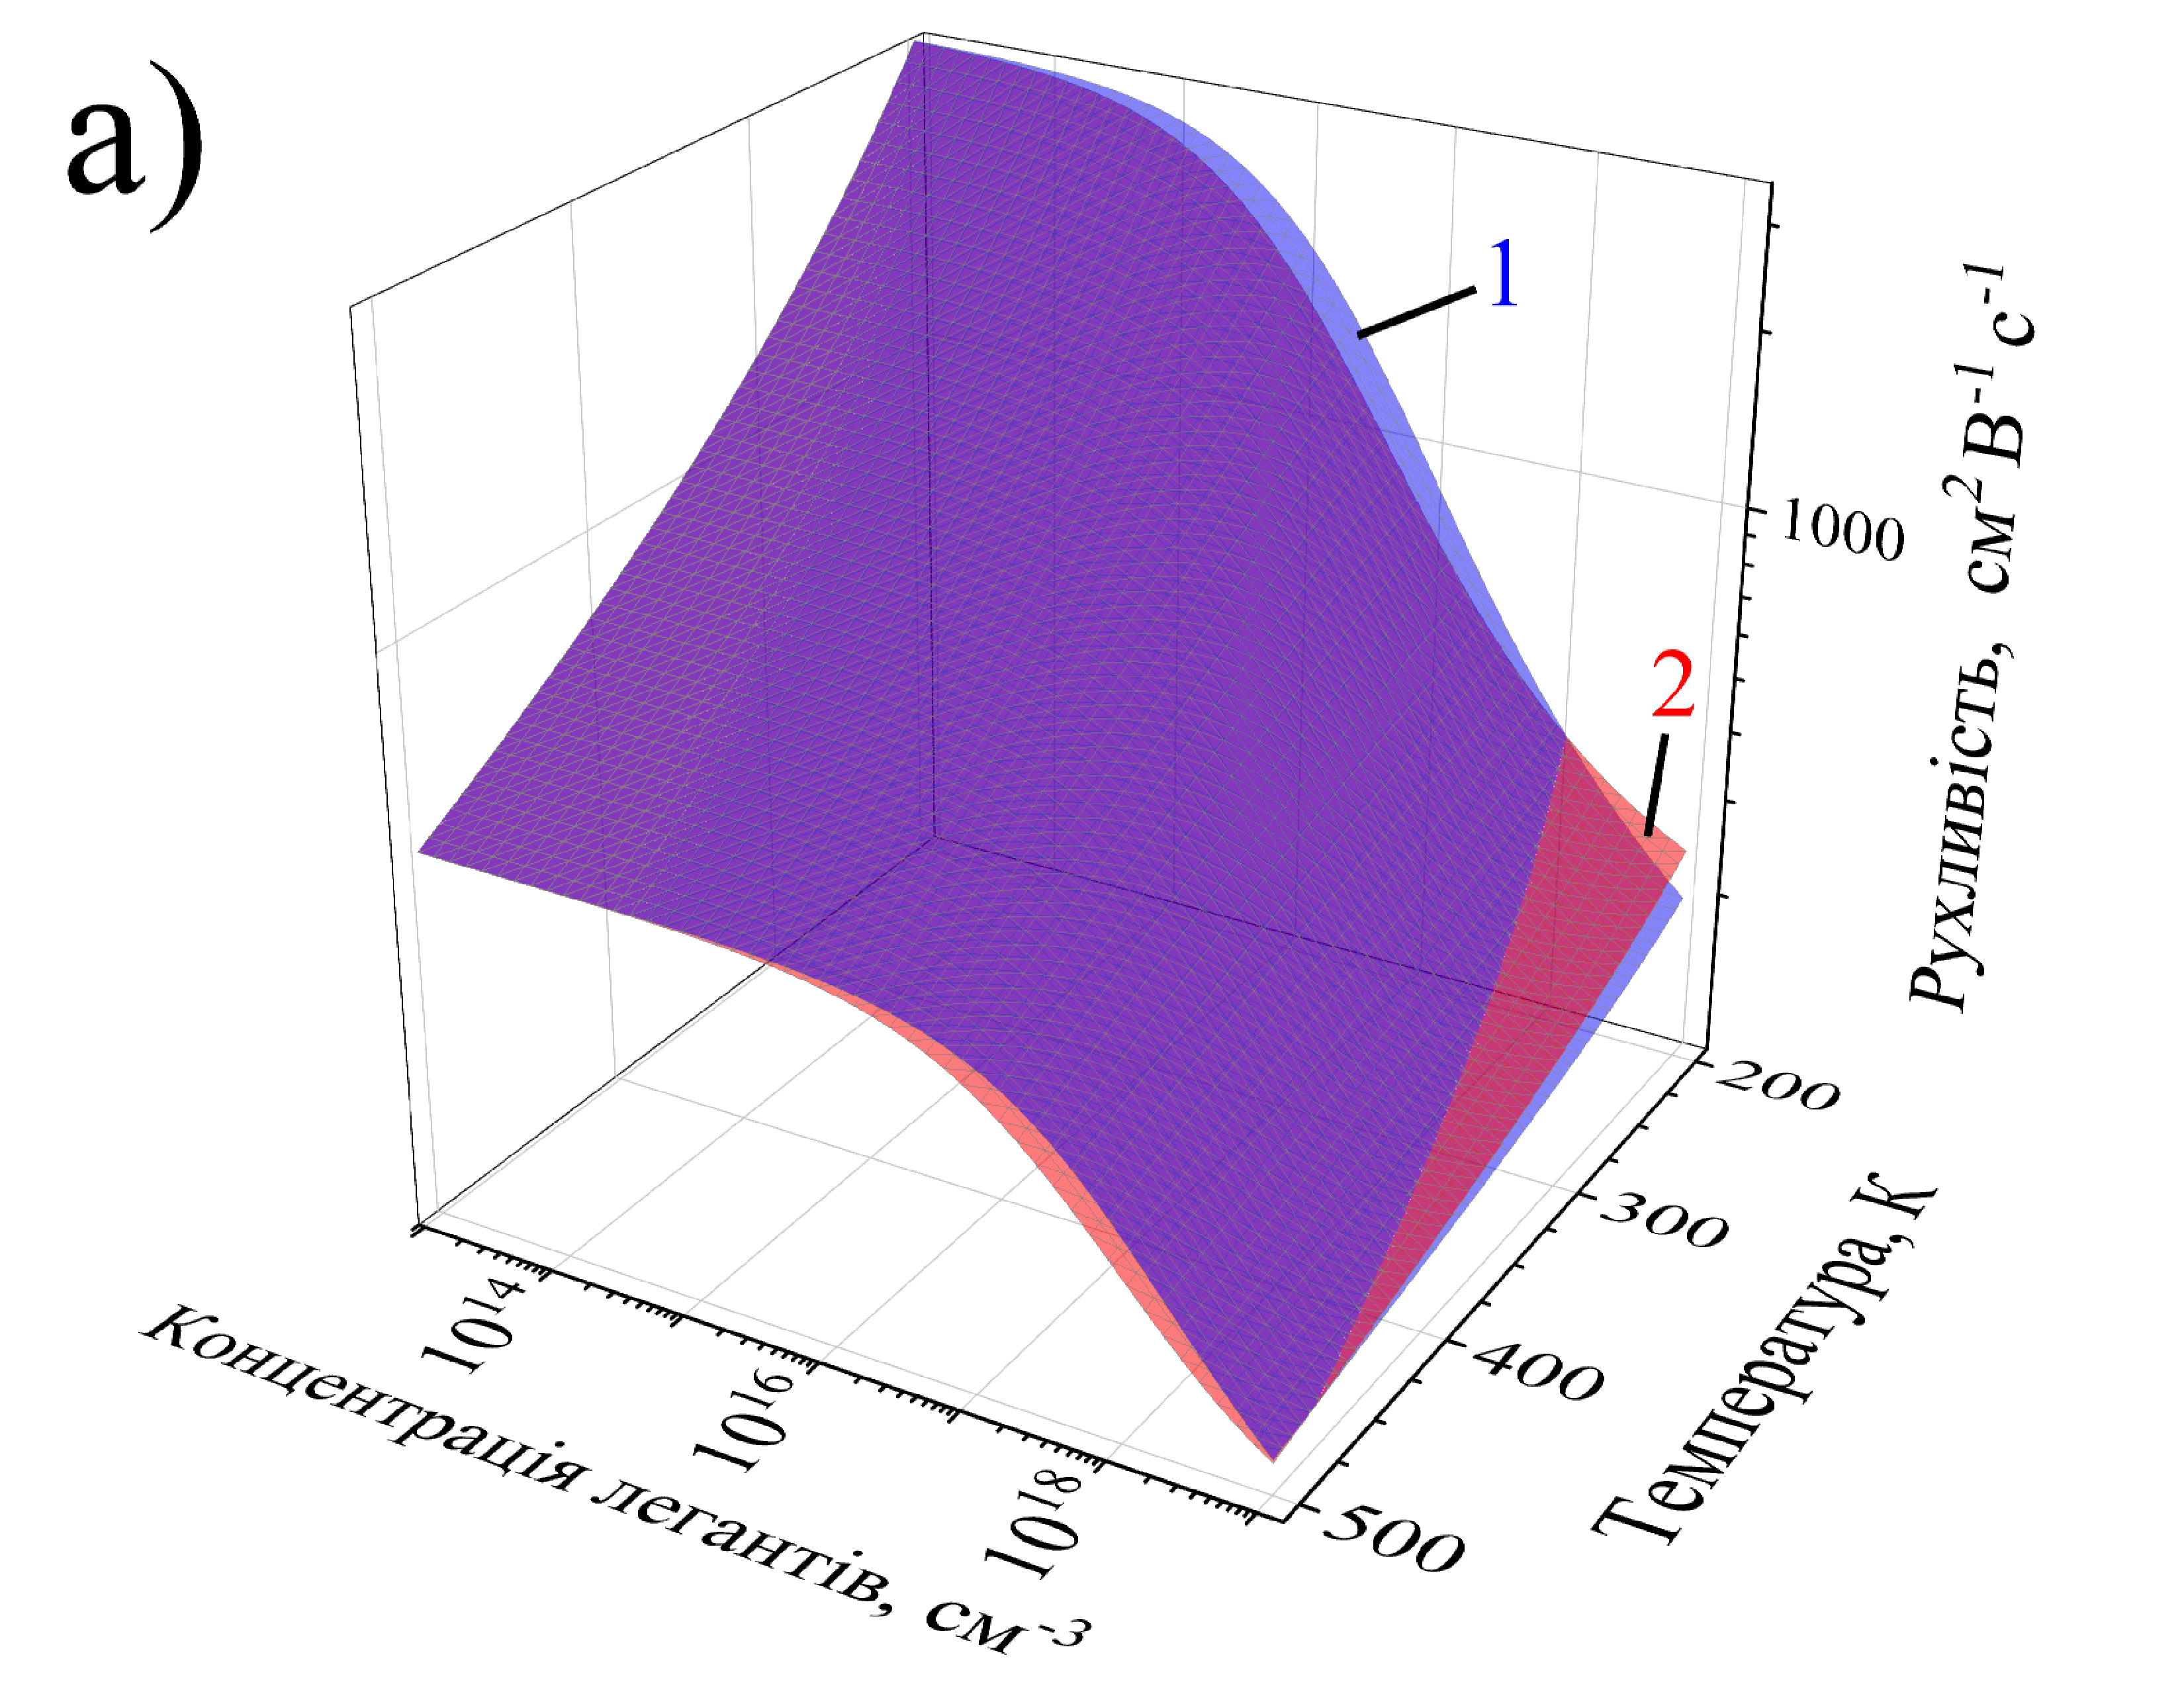
\includegraphics[width=0.49\linewidth]{Fig21a.png}
     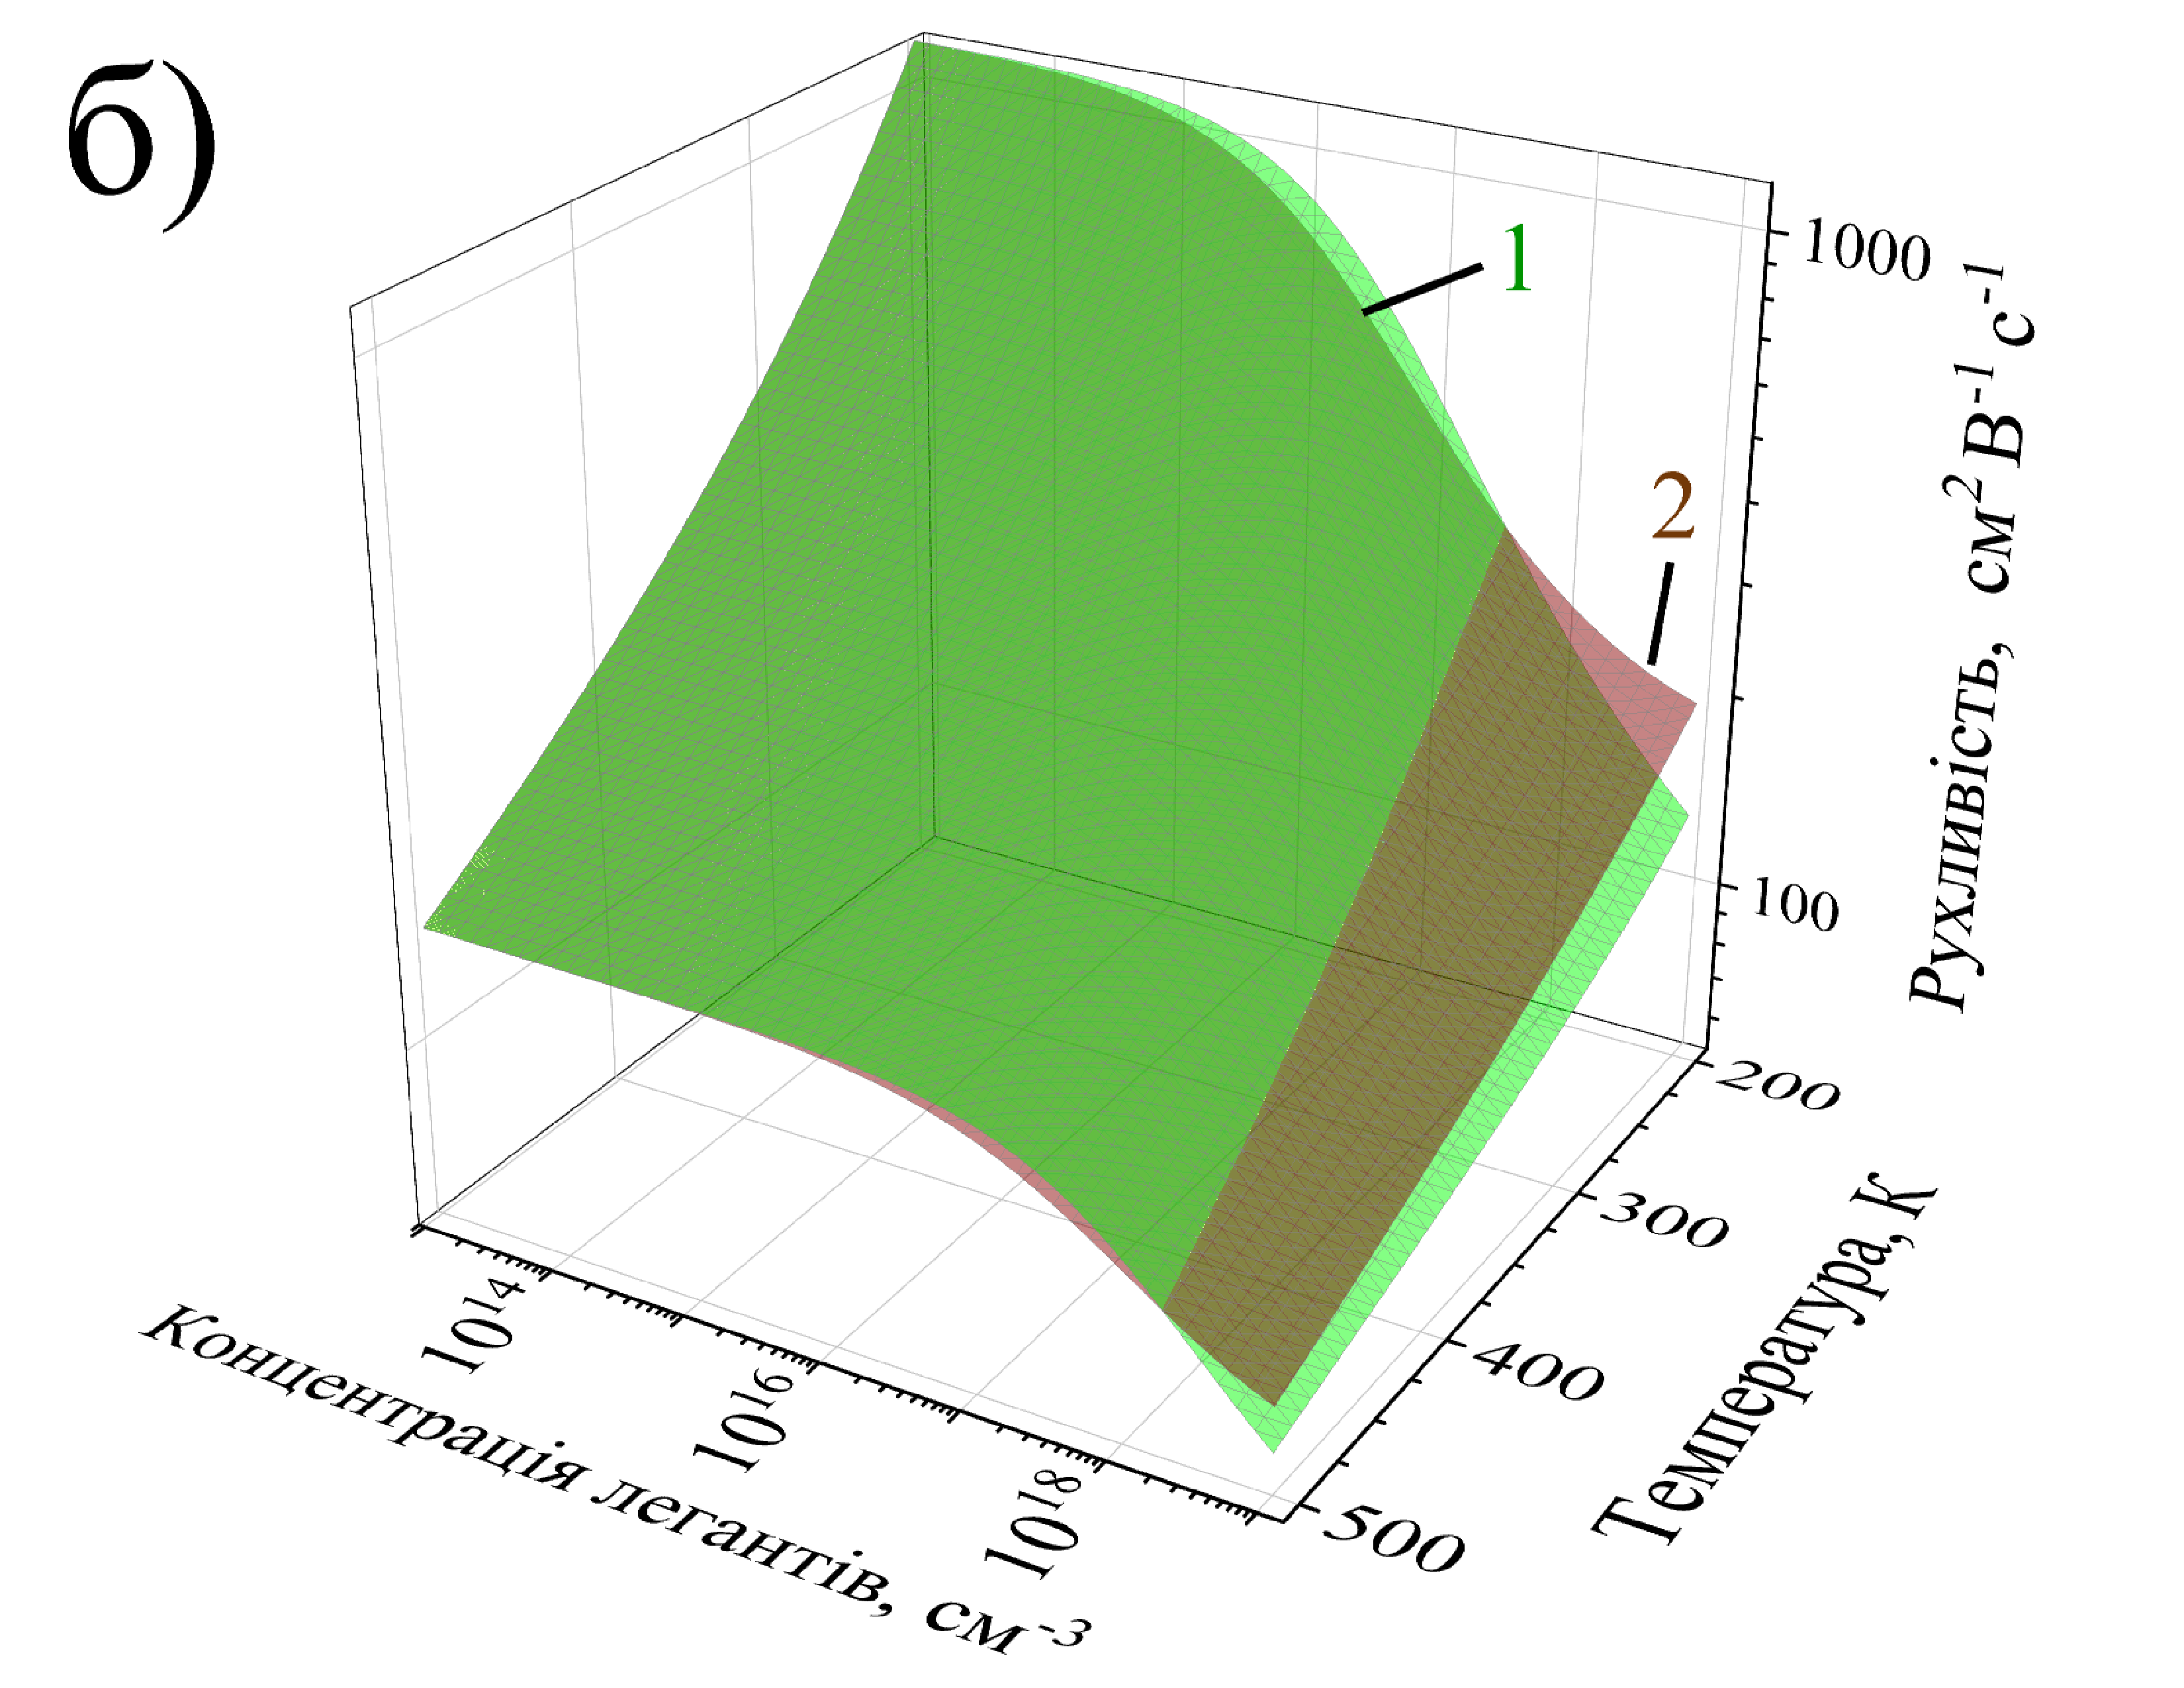
\includegraphics[width=0.49\linewidth]{Fig21b.png}
	  \caption{Залежності рухливості електронів (a) та дірок (б) у випадку, коли вони є основними (поверхні 1) та неосновними (поверхні 2)
носіями заряду від температури та концентрації легуючої домішки. Розрахунки виконані відповідно до теорії Klaassen.
}\label{figMuKl}
\end{figure}

\section{Налаштування Symbolic Regression}

Символьна регресія (Symbolic Regression, SR) --- це достатньо новий алгоритм МН, який апроксимує
залежності між вхідними та вихідними параметрами та дозволяє отримати аналітичний зв'язок між ними у вигляді математичної формули \cite{Angelis2023}.
При побудові функціональної залежності та пошуку числових параметрів використовуються еволюційні алгоритми.
SR є одним із методів, які об'єднують дані, моделі машинного навчання та наукові теорії, дозволяючи отримати аналітичні вирази,
які можуть бути інтерпретовані, дозволяють отримати передбачення дешевши з точки зору обчислень порівняно з класичними моделями МН
та легше інтегруються у вирішення різноманітних фізичних проблем.

При реалізації цього алгоритму використовувався open source пакет PySR, орієнтований на використання мови Python.
Для побудови рівнянь використовувалися стандартні математичні функції
($+$, $-$, $\times$, $\div$, $\exp$, $\ln$, $x^y$, $\tanh$, $\sin$) та дійсні константи.
Крім того використовувалися спеціально сконструйовані оператори
$f_1(x)=\frac{1}{1+x}$ та $f_2(x,y)=\frac{x\cdot y}{x+y}$.
Ці оператори відповідають функціям, які часто зустрічаються в існуючих моделях для опису рухливості носіїв заряду --- див. Розділ~\ref{Teor}.


SR може призвести до складних виразів, які важко інтерпретувати через те, що вони, що містить небажані ознаки, такі як, наприклад,
вкладені операції.
Щоб запобігти цьому застосовувалися обмеження, які забороняли
дві послідовні операції $\sin$ (тобто $\sin(\sin(\bullet))$), $f_1$, $f_2$ та $\tanh$,
а також вкладеність $\tanh$ в $f_1$ та $f_2$,
та $\ln$ і $x^y$ в $\exp$.
Також було заборонено комплексність (складність) показника експоненти вище 3 та показника функції $x^y$ вище 5.

Попередня обробка даних полягала у їхній нормалізації, тобто на вхід SR моделі надходили величини $T_n$ $N_{Dn}$,
пов'язані з реальними температурою та концентрацією легуючої домішки наступним чином:
\begin{subequations} \label{eqNorm}
    \begin{align}
      T_n& = \frac{T}{300\,\text{K}}\,, \label{eqNorma} \\
      N_{Dn}& = \frac{N_D}{10^{17}\,\text{см}^{-3}}\,. \label{eqNormb}
    \end{align}
\end{subequations}

\section{Класичні регресійні моделі}

Окрім символьної регресії, в роботі для оцінки рухливості також були реалізовані декілька моделей, які базуються на використанні
більш класичних алгоритмів МН. А саме, були використані:

\noindent
1)~\emph{Random Forest} (RF)  --- алгоритм, який досягає покращення точності прогнозування
завдяки навчанню декількох дерев рішень на різних підмножинах тренувального набору даних;
RF агрегує прогнози всіх дерев, використовуючи голосування під час класифікації або усереднення у випадку вирішення регресійних завдань (як в нашому випадку),
що дозволяє зменшити перенавчання та підвищуючи стійкість до шуму \cite{Breiman2001};

\noindent
\emph{Gradient Boosting} (GB) ---  об'єднує декілька слабких моделей, як правило, дерев рішень, з метою
покращення ефективності прогнозування;
кожна нова модель виправляє помилки попередньої, тим самим підвищуючи загальну точність;
остаточний прогноз отримують шляхом агрегування прогнозів, зазвичай за допомогою зважено суми \cite{Natekin2013};

\noindent
\emph{Support Vector Regression}(SVR) --- передбачає знаходження функції, яка наближує залежність між вхідними змінними та цільовими значеннями з максимально допустимою похибкою, водночас забезпечуючи якнайменшу складність моделі;
може використовувати різні функції ядра (наприклад, радіально-базисні чи поліноміальні), щоб працювати з нелінійними залежностями \cite{Cao2020};

\noindent
\emph{Deep Neural Network} (DNN) --- складається з декількох шарів взаємопов'язаних нейронів, які обробляють вхідні дані
шляхом послідовних нелінійних перетворень \cite{Liu2023}.

Підкреслимо, що хоча подібні моделі також дозволяють передбачати певні величини (наприклад, рухливість носіїв,
як це відбувалося в нашому випадку), проте вони є фактично чорною скринькою, що суттєво утруднює обґрунтування отриманих результатів
і поступово перестає задовольняти дослідників.


Вказані моделі були імплементовані на мові Python,
використовуючи пакети Keras (для DNN) та Scikit-learn (для RF, GB та and SVR).

Розглядалися два варіанти кожного типу моделей, які відрізнялися попередньою обробкою даних.
В одному випадку як вхідні ознаки використовувалися нормовані значення температури та концентрації легуючої домішки
(визначені відповідно до (\ref{eqNorm})), а прогнози були орієнтовані на отримання величини $\mu$.
Відповідні моделі надалі позначатимуться шляхом додавання до абревіатури використаного алгоритму суфіксу ``\_N'' (RF\_N, DNN\_N тощо)
Проте ознаки достатньо сильно відрізняються за величиною між собою, а $N_D$ ще й змінюється у межах шести порядків,
що може бути перепоною для точних прогнозів.
Тому для другого типу моделей проводилася попередня обробка вхідних ознак, яка передбачала нормалізацію (Z-стандартизацію, вже вибачте за усталений термін)
як значень температури $T$,
так і логарифмів ступеню легування $\lg N_D$
(здійснювалися лінійні перетворення, в результаті яких тренувальні набори кожної з ознак характеризувалися нульовим середнім і одиничним стандартним відхиленням).
Моделі були орієнтовані на передбачення нормалізованих значень $\lg \mu$.
Процес нормалізації був реалізований за допомогою функції StandartScaler з пакету Scikit-learn і позначення відповідних моделей міститиме суфікс ``\_S''.

Відомо, що налаштування гіперпараметрів  є надзвичайно важливим для оптимізації продуктивності моделі \cite{Hanif2024}.
Перелік гіперпараметрів, які налаштовувалися для кожної з моделей, а також діапазони пошуку вказані в Таблицях~\ref{tblRFs}-\ref{tblDNNs}.


\begin{table}
%\setlength{\tabcolsep}{3pt}
\caption{Пошуковий простір гіперпараметрів для RF моделей }
\label{tblRFs}
\centering
\begin{tabular}{|l|c|}
\hline
Гіперпараметр&Можливі значення (діапазон пошуку)\\
\hline
\# estimators&	$100\div700$\\
\hline
max depth&	$10\div70$\\
\hline
min samples leaf &	1, 2, 3, 4, 5\\
\hline
min samples split	&2, 3, 4, 5\\
\hline
bootstrap	& True, False \\
\hline
max features &	0,5, 0,8, 1\\
\hline
\end{tabular}
\end{table}


\begin{table}[!ht]
\caption{Пошуковий простір гіперпараметрів для GB моделей }
\label{tblGBs}
\centering
\begin{tabular}{|l|c|}
\hline
Гіперпараметр&Можливі значення (діапазон пошуку)\\
\hline
\# estimators&	$200\div900$\\
\hline
max depth&	$2\div40$\\
\hline
min samples leaf &	1, 2, 3, 4, 5, 6, 7\\
\hline
min samples split	&2, 3, 4, 5, 6, 7\\
\hline
learning rate	& $10^{-3}\div1$ \\
\hline
max features &	0,5, 0,6, 0,7, 0,8, 0,9, 1\\
\hline
\end{tabular}
\end{table}

\begin{table}[!ht]
\caption{Пошуковий простір гіперпараметрів для SVR моделей }
\label{tblSVRs}
\centering
\begin{tabular}{|l|c|}
\hline
Гіперпараметр&Можливі значення (діапазон пошуку)\\
\hline
kernel &	linear, poly, rbf, sigmoid\\
\hline
degree$^*$&	2, 3, 4, 5, 6\\
\hline
$C_0$ &	$0-8$\\
\hline
Tolerance	&$10^{-5}\div10^{-2}$\\
\hline
$C$	& $10^{-2}\div15$ \\
\hline
$\varepsilon$ &	$10^{-4}\div0,5$\\
\hline
\multicolumn{2}{l}{$^*$ лише для kernel=poly}\\
\end{tabular}
\end{table}

\begin{table}[!ht]
\caption{Пошуковий простір гіперпараметрів для DNN моделей }
\label{tblDNNs}
\centering
\begin{tabular}{|l|c|}
\hline
Гіперпараметр&Можливі значення (діапазон пошуку)\\
\hline
\# nodes for first hidden layer &$5\div150$\\
\hline
batch size&	1, 4, 16\\
\hline
activation function &	ReLu, sigmoid, tanh, SELU, ELU\\
\hline
%optimizer	&\makecell{SGD, RMSprop, Adam, Adadelta, \\Adagrad, Adamax, Nadam, Ftrl}\\
optimizer	&SGD, RMSprop, Adam, Adadelta, Adagrad, Adamax, Nadam, Ftrl\\
\hline
learning rate	& $10^{-4}\div10^{-2}$ \\
\hline
%weight initializer &	\makecell{Xavier Normal, Xavier Uniform, \\He Normal, He Uniform, \\Random Normal, Random Uniform}\\
weight initializer &	\makecell{Xavier Normal, Xavier Uniform, He Normal, He Uniform, \\Random Normal, Random Uniform}\\
\hline
\end{tabular}
\end{table}

Зазначимо, що у випадку DNN вхідний шар складався з двох вузлів, вихідний містив один вузол,
а структура схованих повнозв'язних шарів наведена на Рис.~\ref{figDNNc}.
Як видно з рисунку, використовувалося шість схованих шарів, кількість вузлів у яких поступово зменшувалося:
від шару до шару на 10\% від кількості вузлів у першому схованому $N_{n1l}$), яка була одним із гіперпараметрів, що налаштовувалися.


\begin{figure}
	\centering
     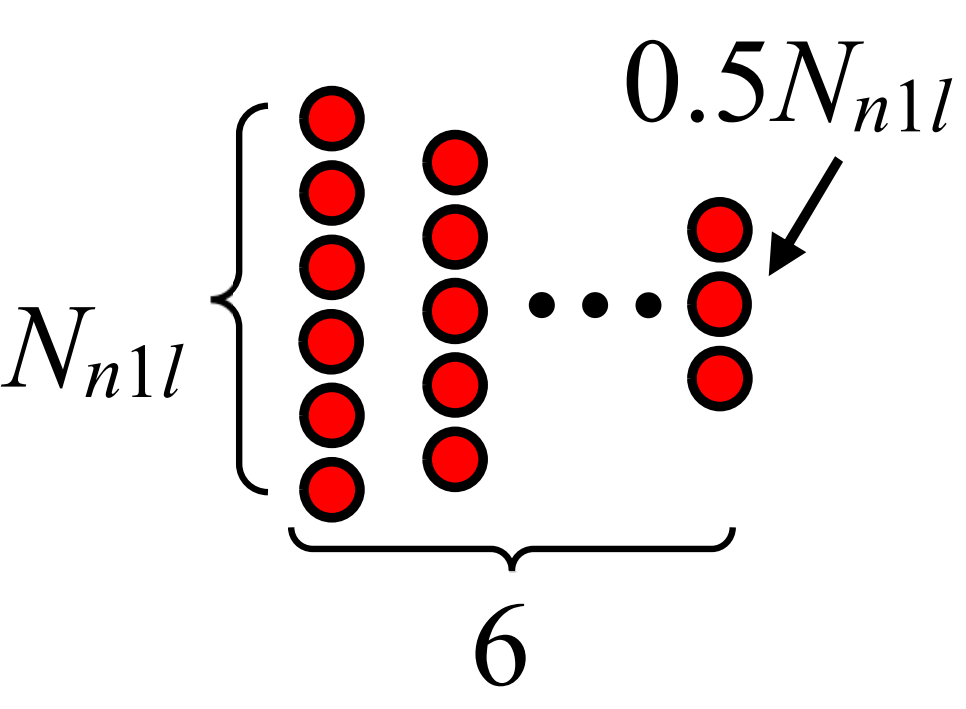
\includegraphics[width=0.5\linewidth]{Fig22.png}
	  \caption{Конфігурація схованих шарів для використаних DNN моделей.
}\label{figDNNc}
\end{figure}

Налаштування моделей здійснювалося за допомогою пакету Optuna \cite{Akiba2019} з використанням TPE самплера та Hyperband прюнера
для ефективного вибору гіперпараметрів.
Під час налаштування використовувалась 5-кратна крос-валідація, яка передбачала почергове використання кожних 20\% тренувального набору
як валідаційних даних для оцінки ефективності моделей, навчених з використанням решти 80\%.




\section{Метрики оцінювання}

To build a regression model, it is crucial to evaluate its performance using various metrics.
These metrics assess how well the model has learned and predicted outcomes.
The evaluation metrics for iron quantification were the mean squared error (MSE),

and coefficient of determination (R$^2$), 

\begin{equation}
\label{eqMSE}
    \mathrm{MSE} = \frac{1}{N}\displaystyle\sum_{i=1}^{N} (\hat{y_i}-y_i)^2\,,
\end{equation}
where $\hat{y_i}$ represents the predicted value for the $i$--th data point,
$y_i$ is the known value for the $i$--th data point,
and $N$ is the number of samples in the dataset.
MSE is one of the most commonly used metrics for evaluating model accuracy.
However, since the computation of $\hat{y_i}$ involves the normalization and logarithm transformation of $N_\mathrm{Fe}$,

%Weights=1/Ytest
%
%X1 = np.expand_dims(np.log10(DT.XInverseNormalize(Xtest)[:, 1]), axis=1)
%
%
%Weights1 = Weights * (X1 **1)

Therefore, we used MAPE, which determines the mean relative error:
\begin{equation}
\label{eqMAPE}
    \mathrm{MAPE} = \frac{1}{N}\displaystyle\sum_{i=1}^{N} \frac{|\mu^\mathrm{PRED}_i-\mu^\mathrm{TRUE}_i|}{\mu^\mathrm{TRUE}_i}\times 100 \%\,,
\end{equation}
where $\mu^\mathrm{PRED}_i$ is the predicted value of iron concentration,
$\mu^\mathrm{TRUE}_i$ is the known value (used in simulation or obtained from experimental iron determination).
mean absolute percentage error (MAPE),

$\mathrm{APE}_\mathrm{MAX}$, 
$\mathrm{APE}_\mathrm{MED}$, 

\begin{equation}
\label{eqMAE}
    \mathrm{MAE} = \frac{1}{N}\displaystyle\sum_{i=1}^{N} |\mu^\mathrm{PRED}_i-\mu^\mathrm{TRUE}_i|\,,
\end{equation}


\chapter{Отримані результати}

\section{Символьна регресія}

\begin{subequations} \label{eqNN}
    \begin{align}
      \mu_{n,n}& =\frac{N_{Dn}+1413,2}{T_n^{2,2508}+\frac{a_{n,n}\cdot b_{n,n}}{a_{n,n}+b_{n,n}}}\,, \label{eqNNa} \\
      a_{n,n} &=\left(\frac{N_{Dn}}{0,873T_n+0,0727}\right)^{0,7212}\,, \label{eqNNb} \\
      b_{n,n}& =0,215N_{Dn}^{0,58}+10,5T_n-1,342\,, \label{eqNNc}
    \end{align}
\end{subequations}

\begin{subequations} \label{eqNP}
    \begin{align}
      \mu_{n,p}& =26,3\cdot\left(\frac{N_{Dn}}{N_{Dn}+192}\right)^{0,62}+\frac{1412,3}{T_n^{2,25}+\frac{a_{n,p}\cdot b_{n,p}}{a_{n,p}+b_{n,p}}}\,, \label{eqNPa} \\
      a_{n,p} &=1,92\cdot\left(\frac{N_{Dn}}{T_n+0,071}\right)^{0,717}\,, \label{eqNPb} \\
      b_{n,p}& =5,7N_{Dn}^{0,103}\cdot T_n\,, \label{eqNPc}
    \end{align}
\end{subequations}


\begin{subequations} \label{eqPP}
    \begin{align}
      \mu_{p,p}& =N_{Dn}^{0,448}+\frac{470}{T_n^{2,2505}+\frac{a_{p,p}\cdot b_{p,p}}{a_{p,p}+b_{p,p}}}\,, \label{eqPPa} \\
      a_{p,p} &=2,652 N_{Dn}^{0,1669}\cdot T_n\,, \label{eqPPb} \\
      b_{p,p}& =0,578 N_{Dn}^{0,7587}\cdot T_n^{-0,755}\,, \label{eqPPc}
    \end{align}
\end{subequations}


\begin{subequations} \label{eqPN}
    \begin{align}
      \mu_{p,n}& =\frac{0,0226N_{Dn}\cdot\ln T_n}{\ln T_n+0,63}
      +\frac{113,56}{\left[0,15617T_n^{2,94}+\left(\frac{a_{p,n}\cdot b_{p,n}}{1,151a_{p,n}+ 4,21 b_{p,n}}\right)^{1,177}\right]^{0,76547}}\,, \label{eqPNa} \\
      a_{p,n} &=N_{Dn}^{0,6085}\,, \label{eqPNb} \\
      b_{p,n}& =T_n^{1,143}\,. \label{eqPNc}
    \end{align}
\end{subequations}


\begin{figure}
	\centering
     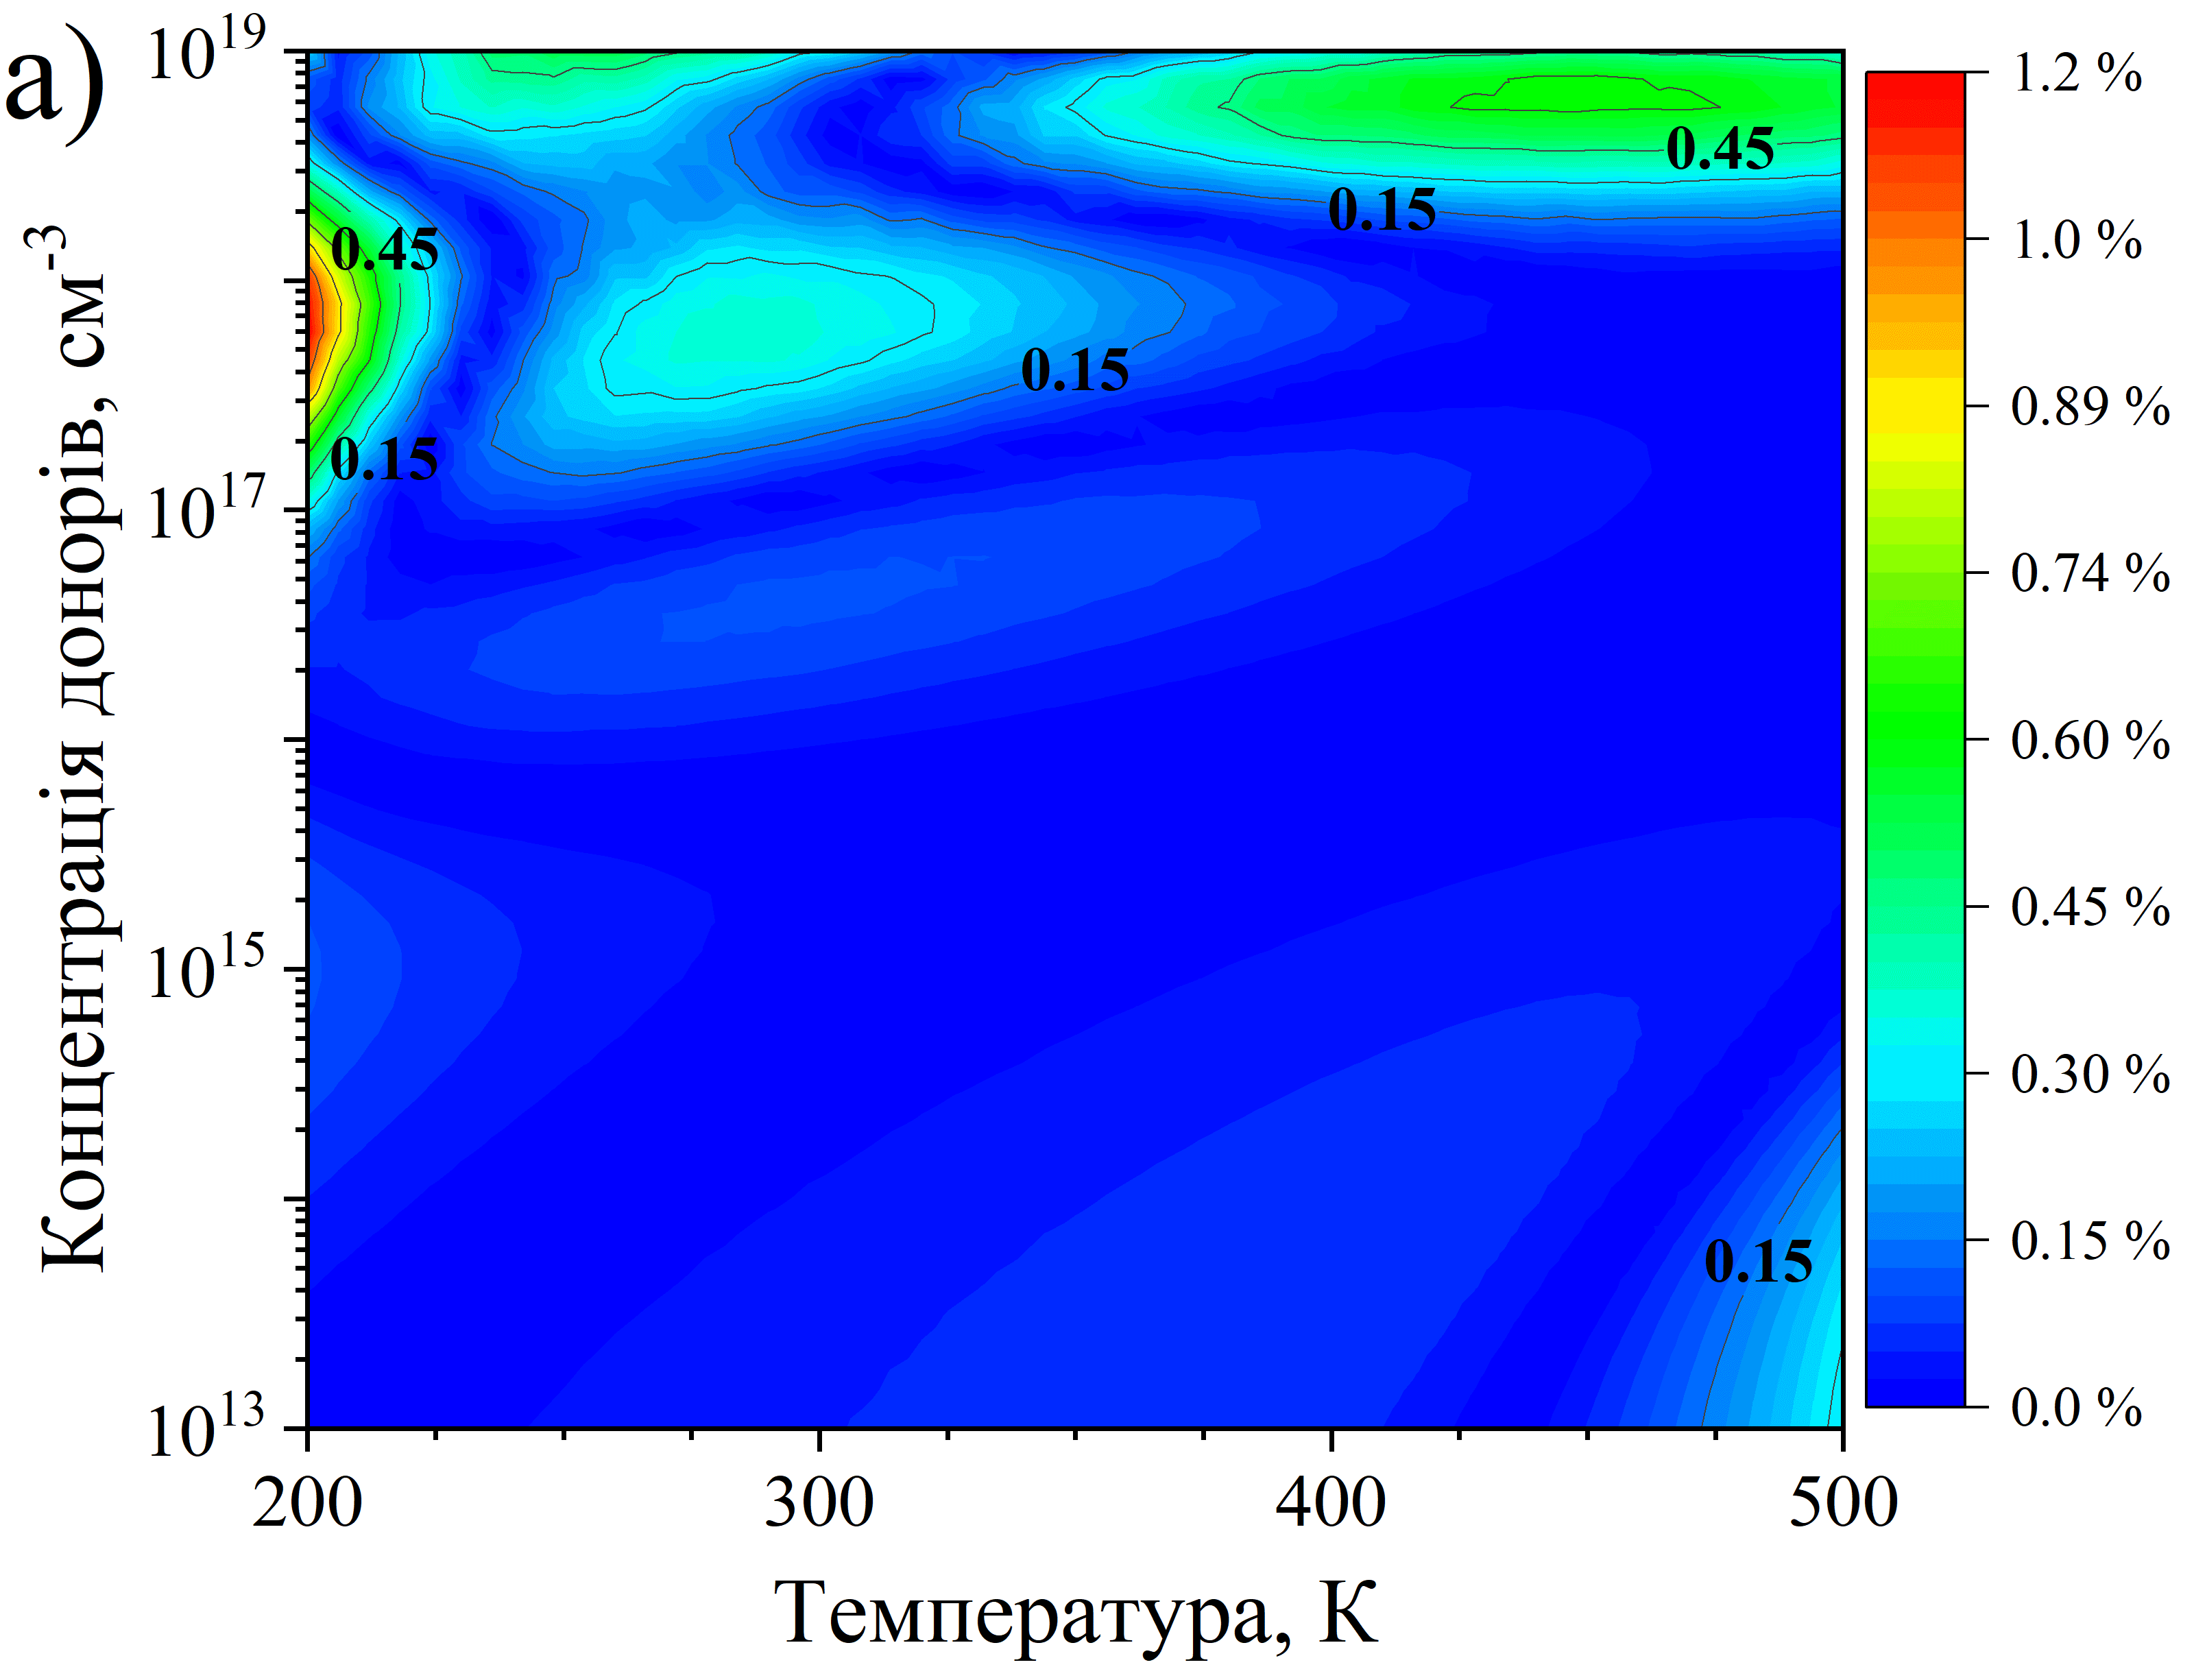
\includegraphics[width=0.49\linewidth]{Fig31a.png}
     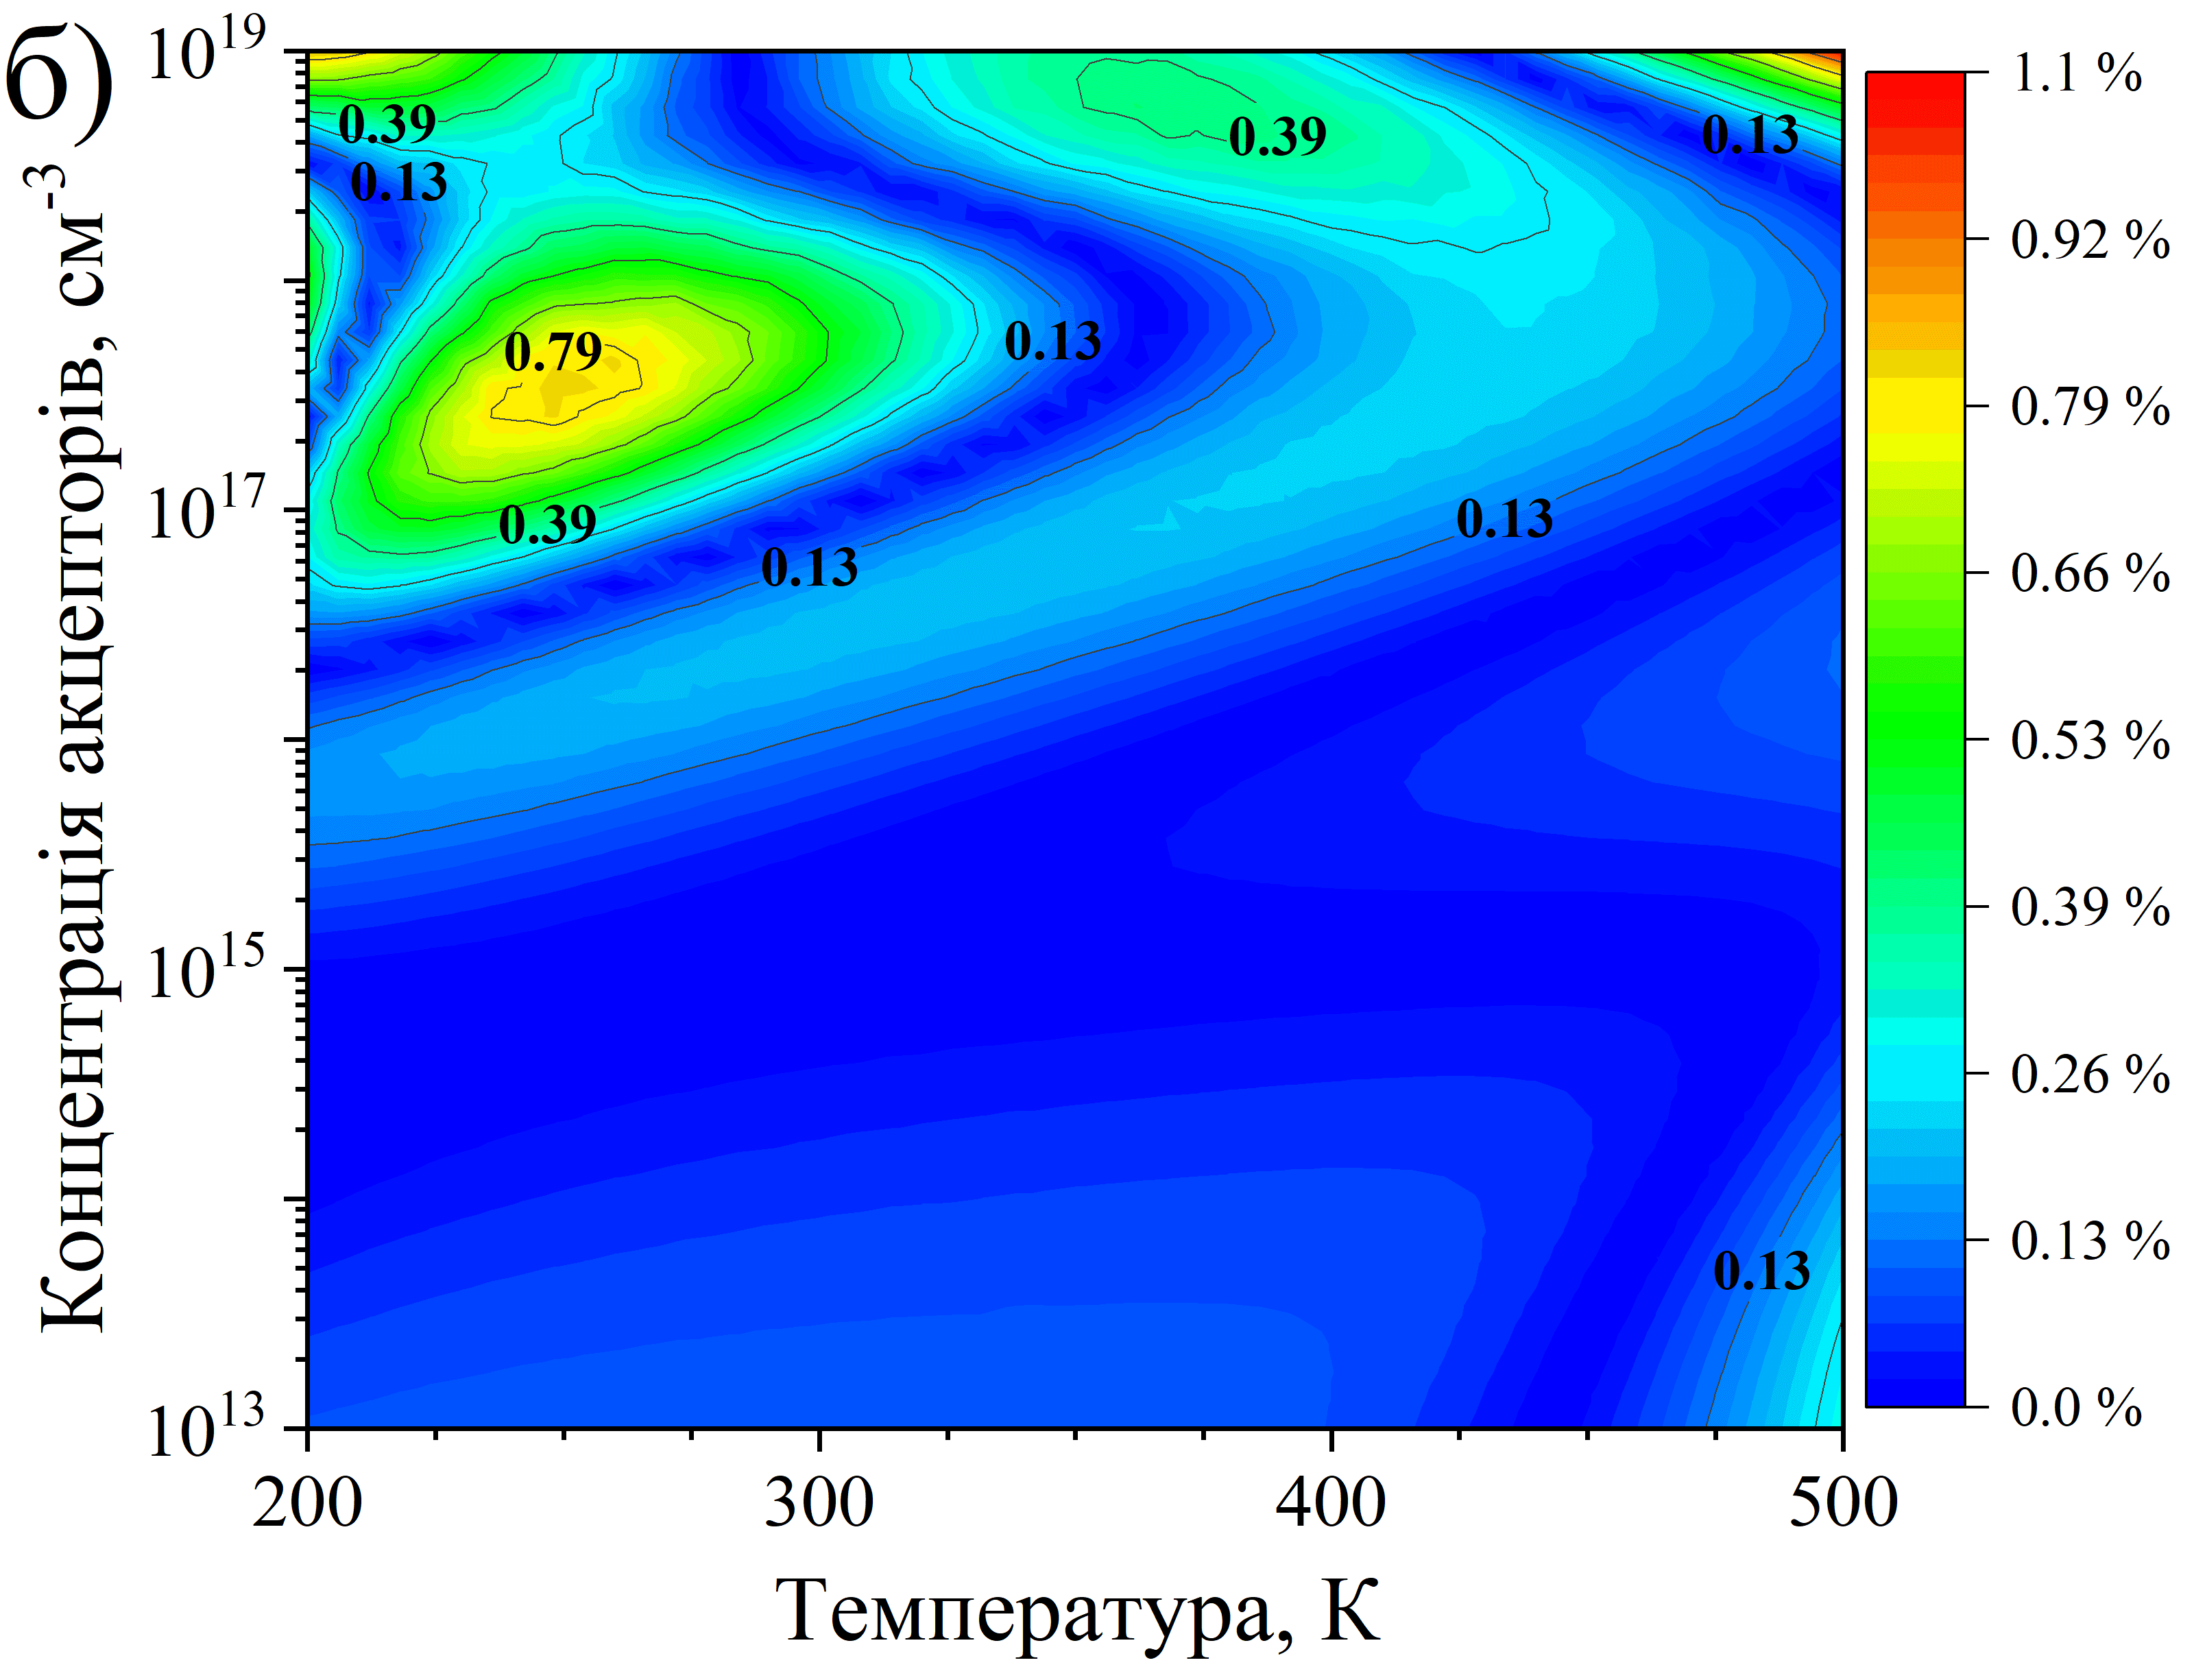
\includegraphics[width=0.49\linewidth]{Fig31b.png}
     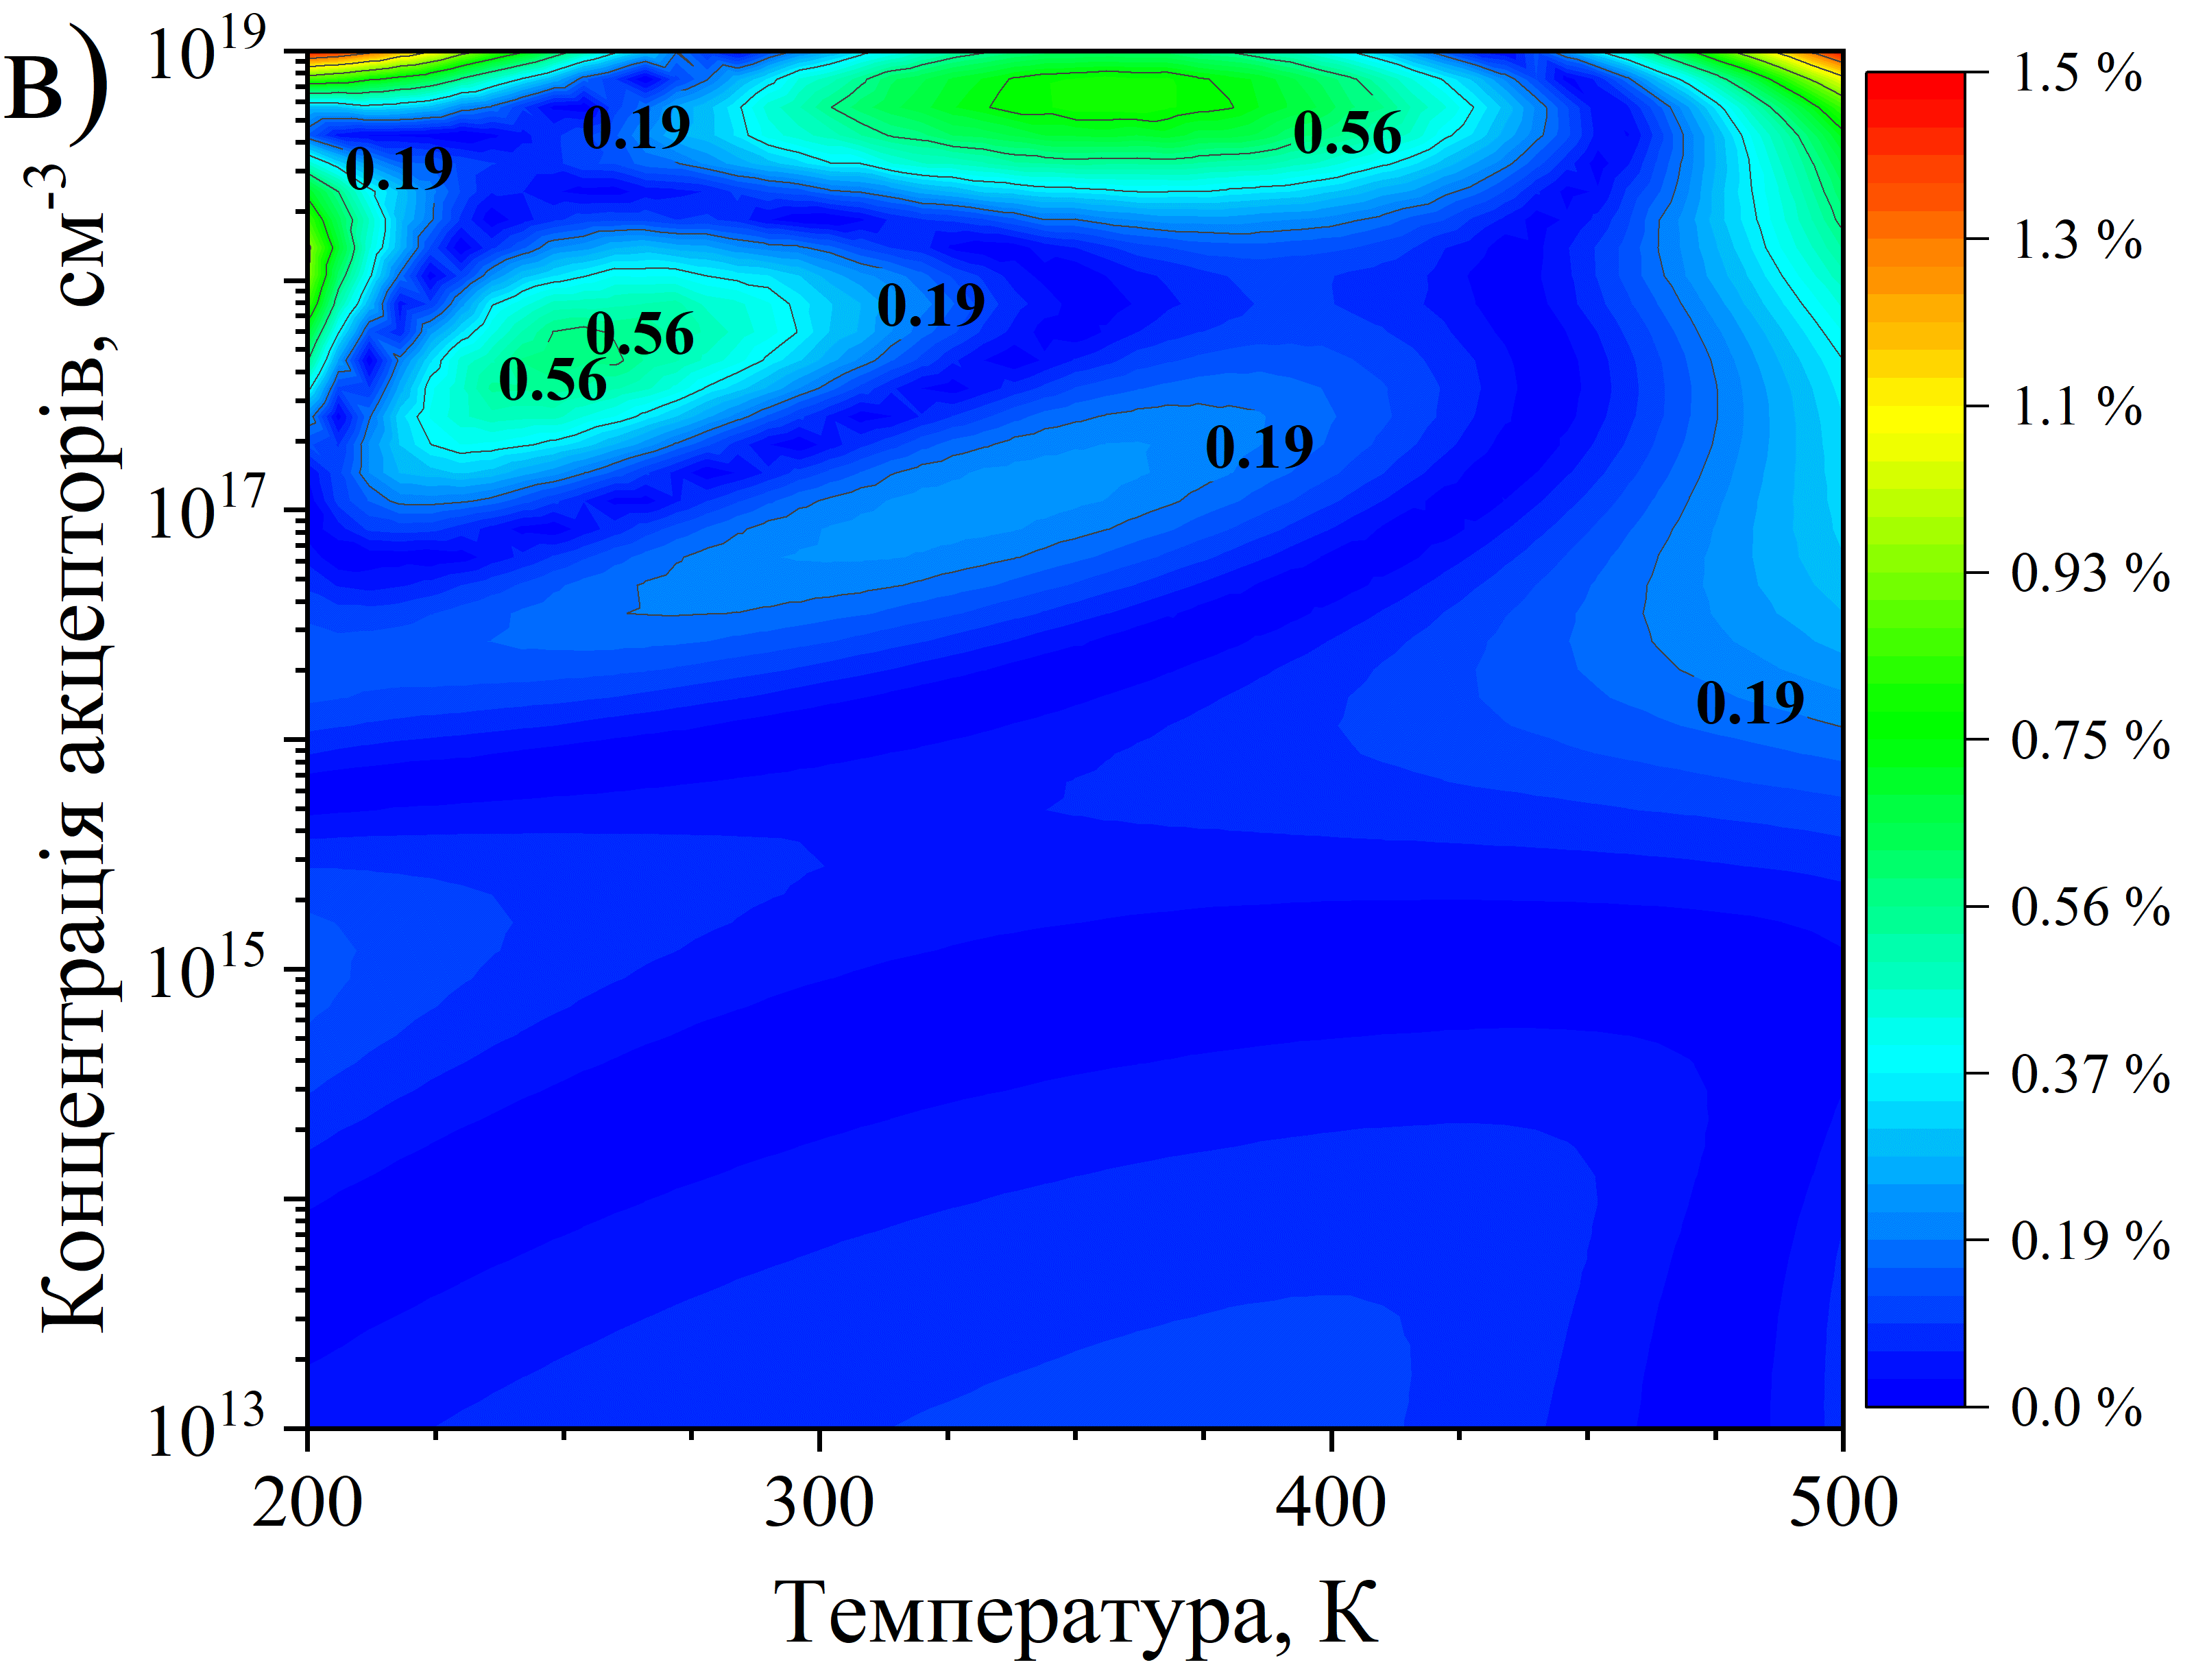
\includegraphics[width=0.49\linewidth]{Fig31c.png}
     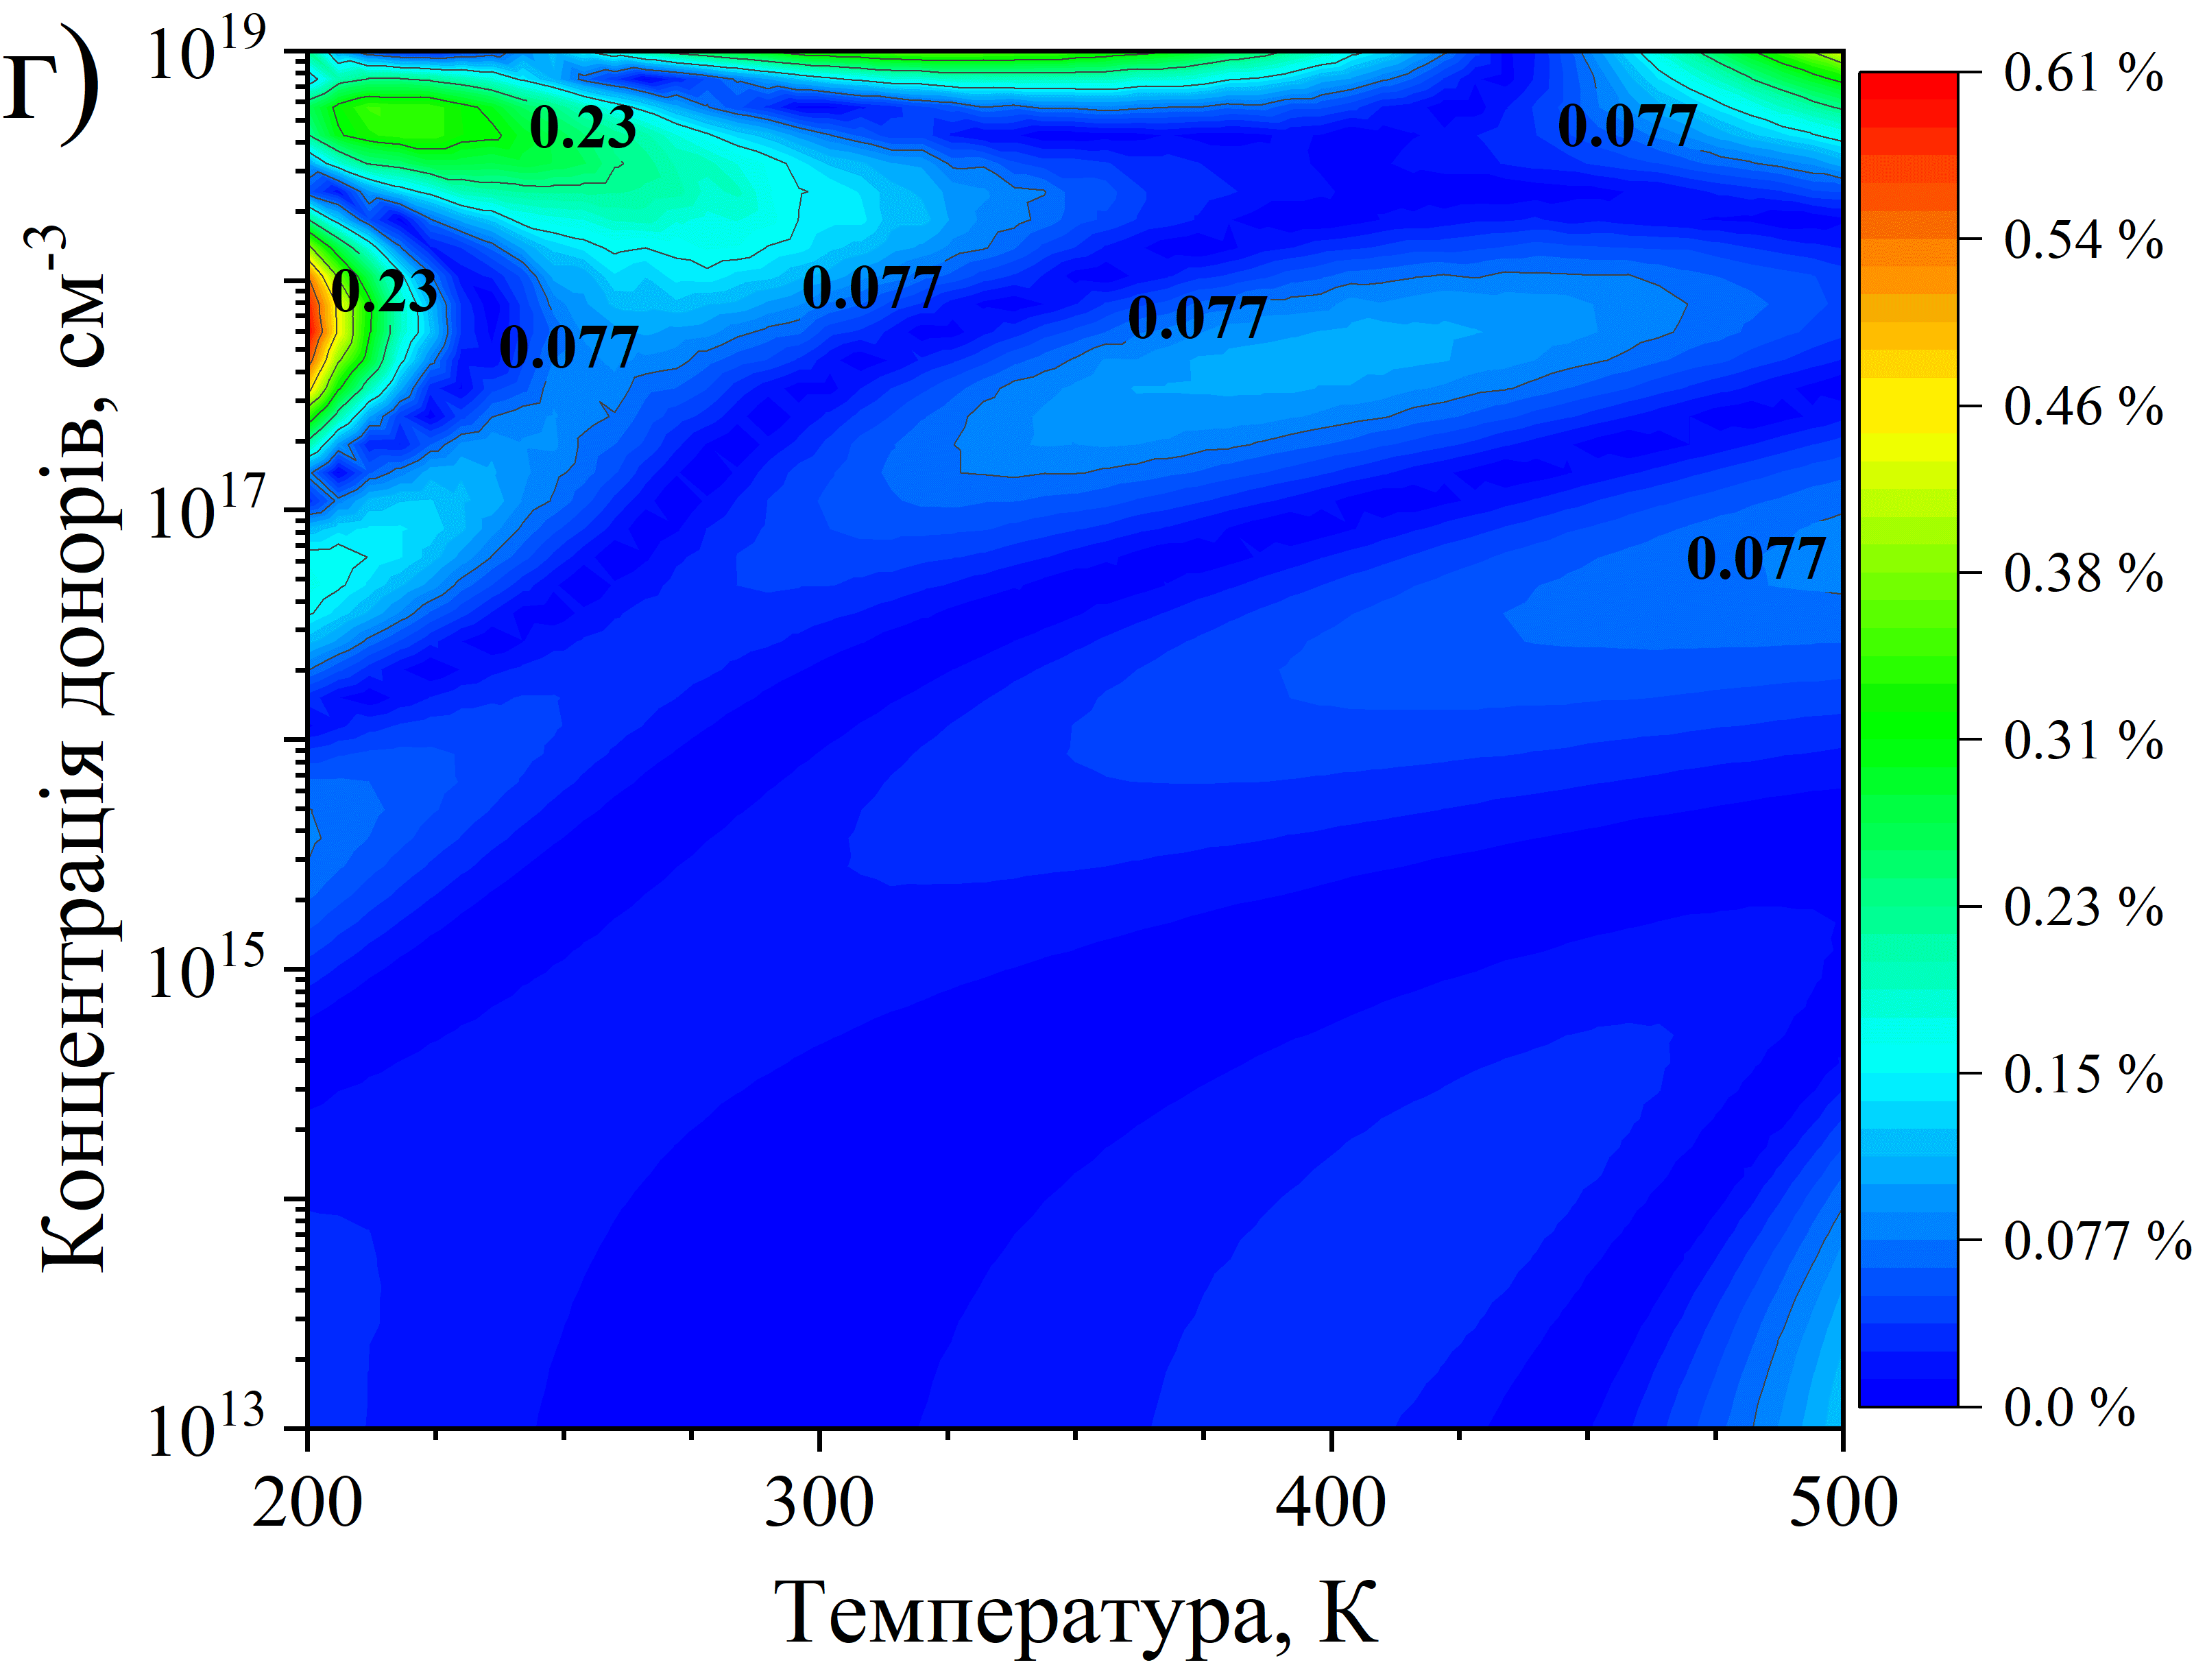
\includegraphics[width=0.49\linewidth]{Fig31d.png}
	  \caption{Залежності величини відносної похибки при оцінці рухливості носіїв заряду 
у кремнії за допомогою виразів (\ref{eqNN}) -- (\ref{eqPN}),
отриманих за допомогою символьної регресії, від температури та рівня легування.
Представлені випадки оцінки рухливості електронів (а, б) та дірок (в, г), коли вони є
основними (а, в) та неосновними (б, г) носіями заряду.
}\label{figSR}
\end{figure}

Умова повної іонізації донорної домішки відповідає положенню рівня Фермі на декілька $kT$
нижче рівня домішки
Температура при якій $E_F=E_d$

температура виснаження
\begin{equation}\label{eqTs}
  n-\text{тип}:\;T_s=\frac{E_d}{k\ln(N_C/N_d)};\quad p-\text{тип}:\;T_s=\frac{E_d}{k\ln(N_V/N_a)}\,.
\end{equation}

%\begin{subequations} \label{eqK5}
%    \begin{align}
%       \text{електрони:} \quad& N_\mathrm{eff} =N_d^+ + N_a^- \cdot G_n(P_n,T) +\frac{p}{F_n(P_n,T)}\,, \label{eqK5a} \\
%        \text{дірки:} \quad& N_\mathrm{eff}= N_a^- + N_d^+ \cdot G_p(P_p,T) +\frac{n}{F_p(P_p,T)}\,. \label{eqK5b}
%    \end{align}
%\end{subequations}

температура початку власної провідності:
\begin{equation}\label{eqTi}
  T_i=\frac{E_G}{k \ln\left(\frac{N_C N_V}{N_D^2}\right)}
\end{equation}

\begin{figure}
	\centering
     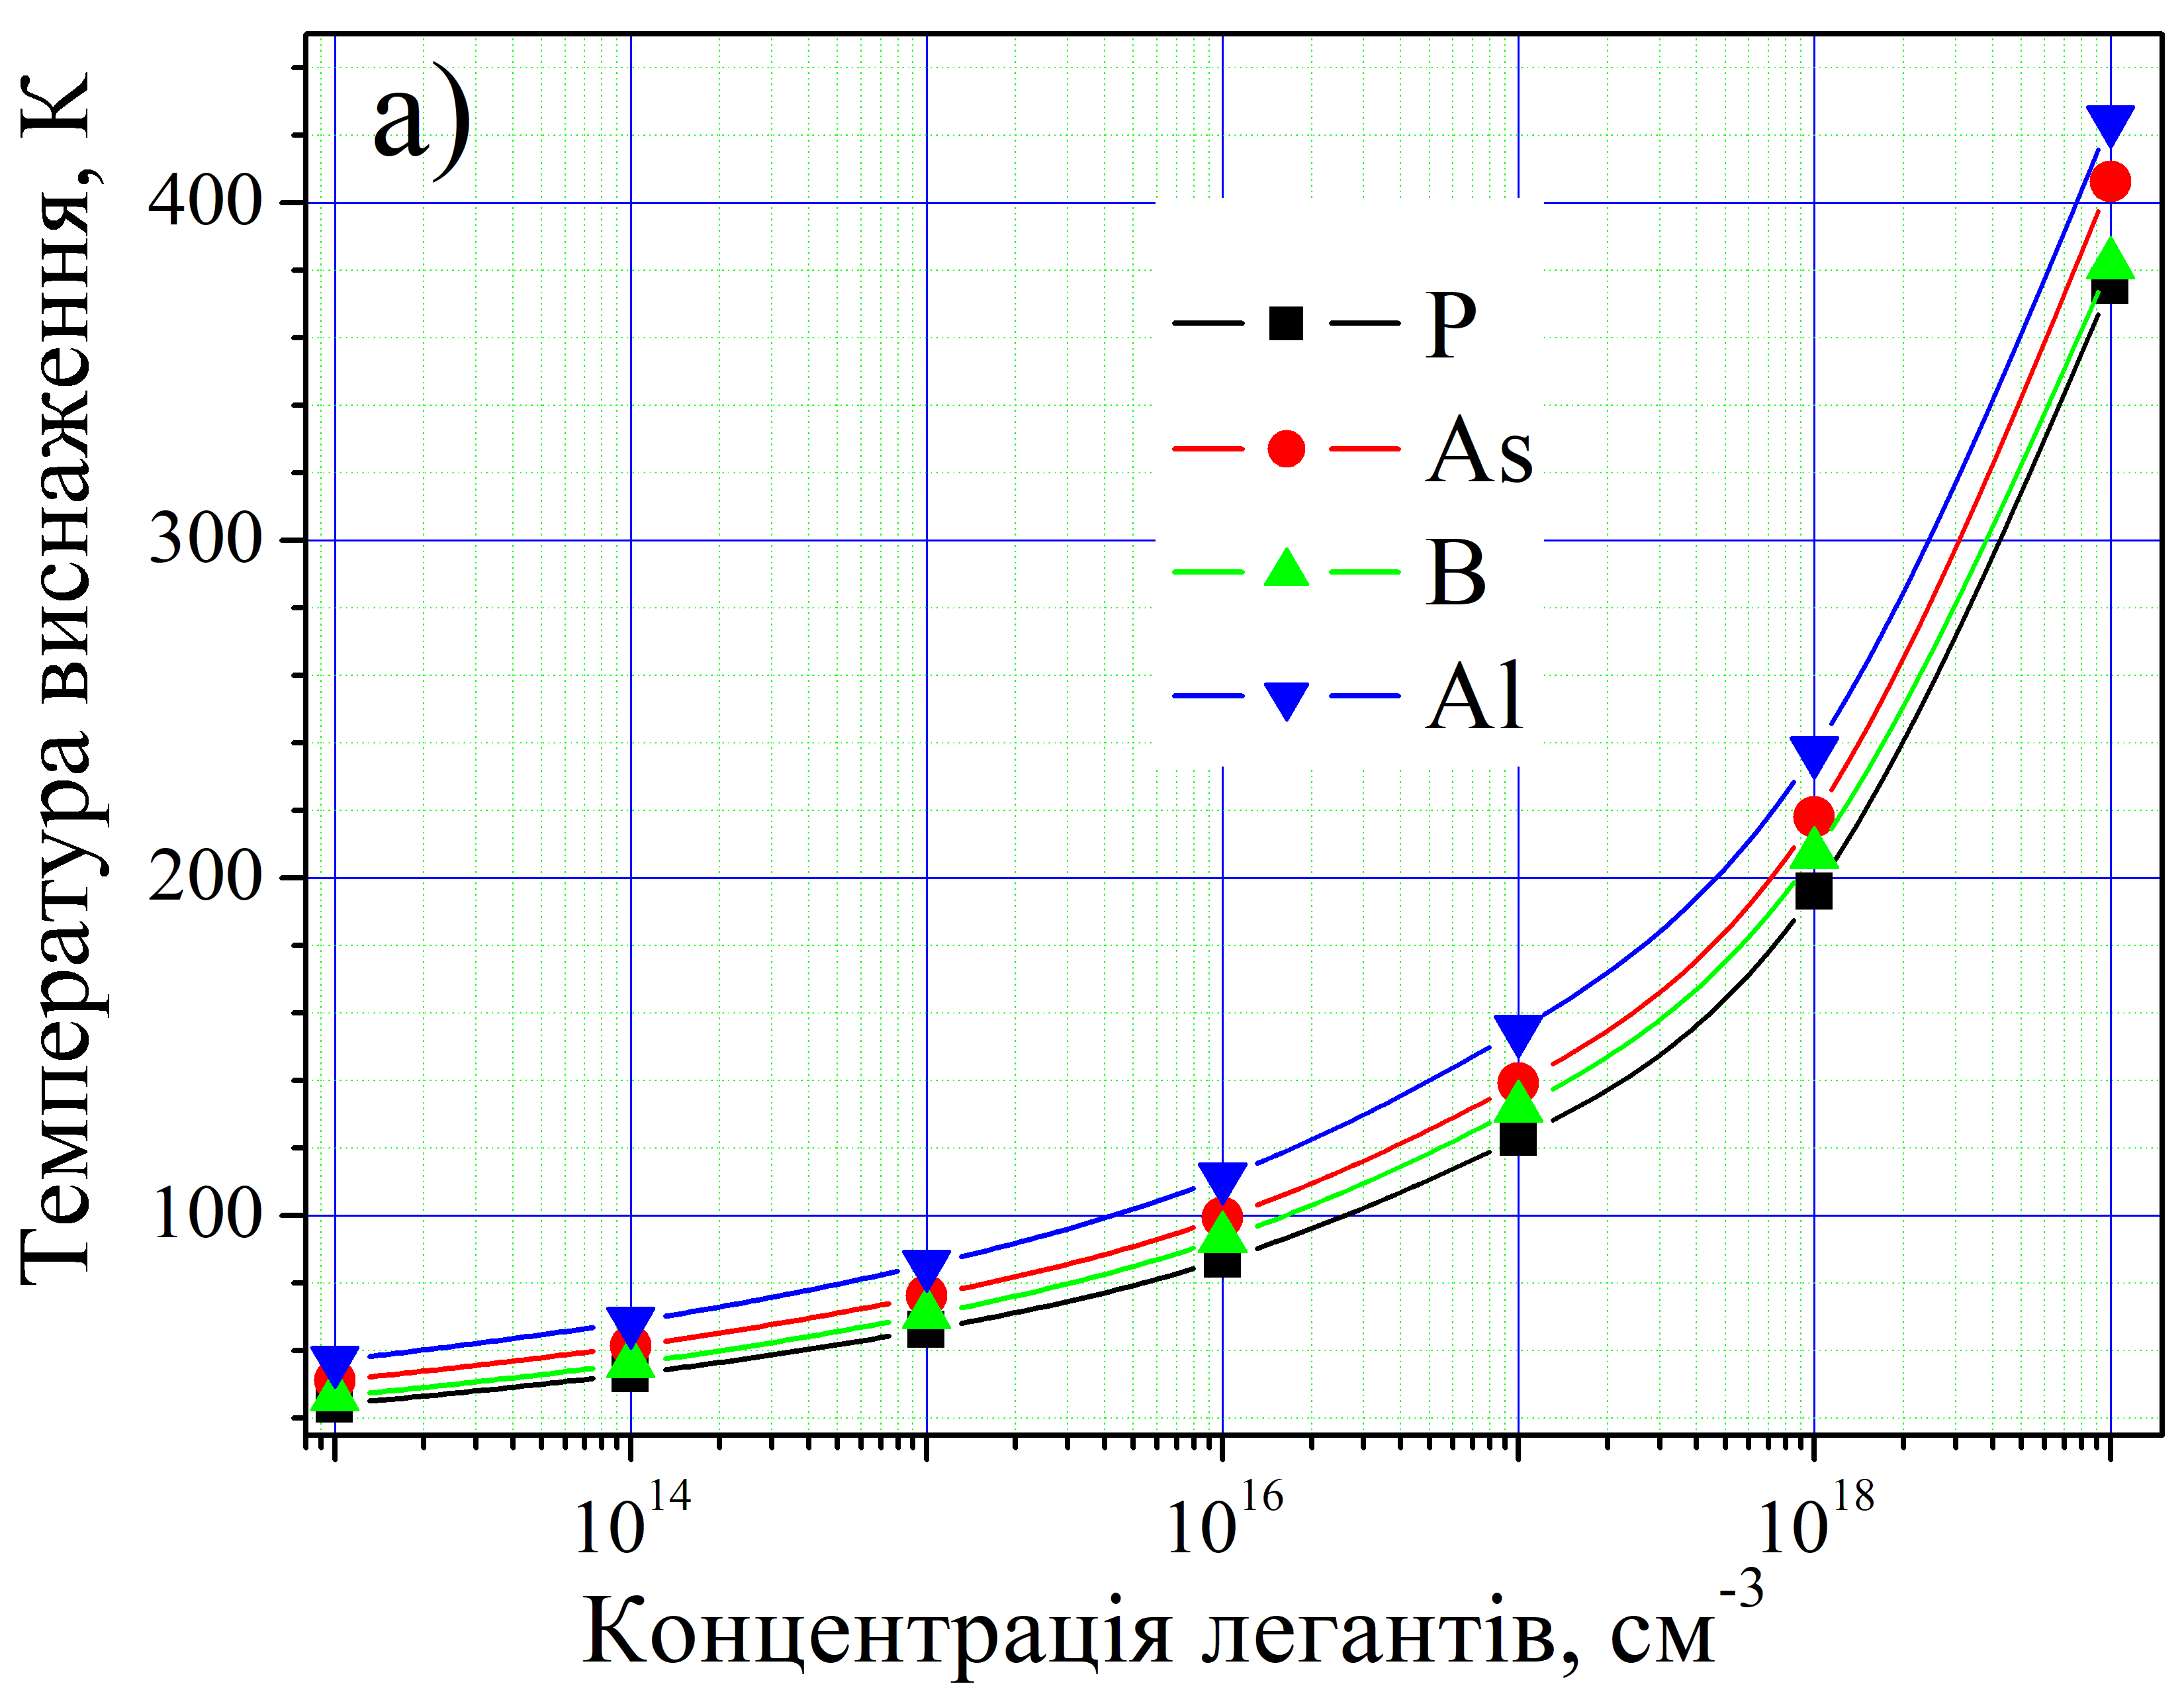
\includegraphics[width=0.49\linewidth]{FigTs.png}
     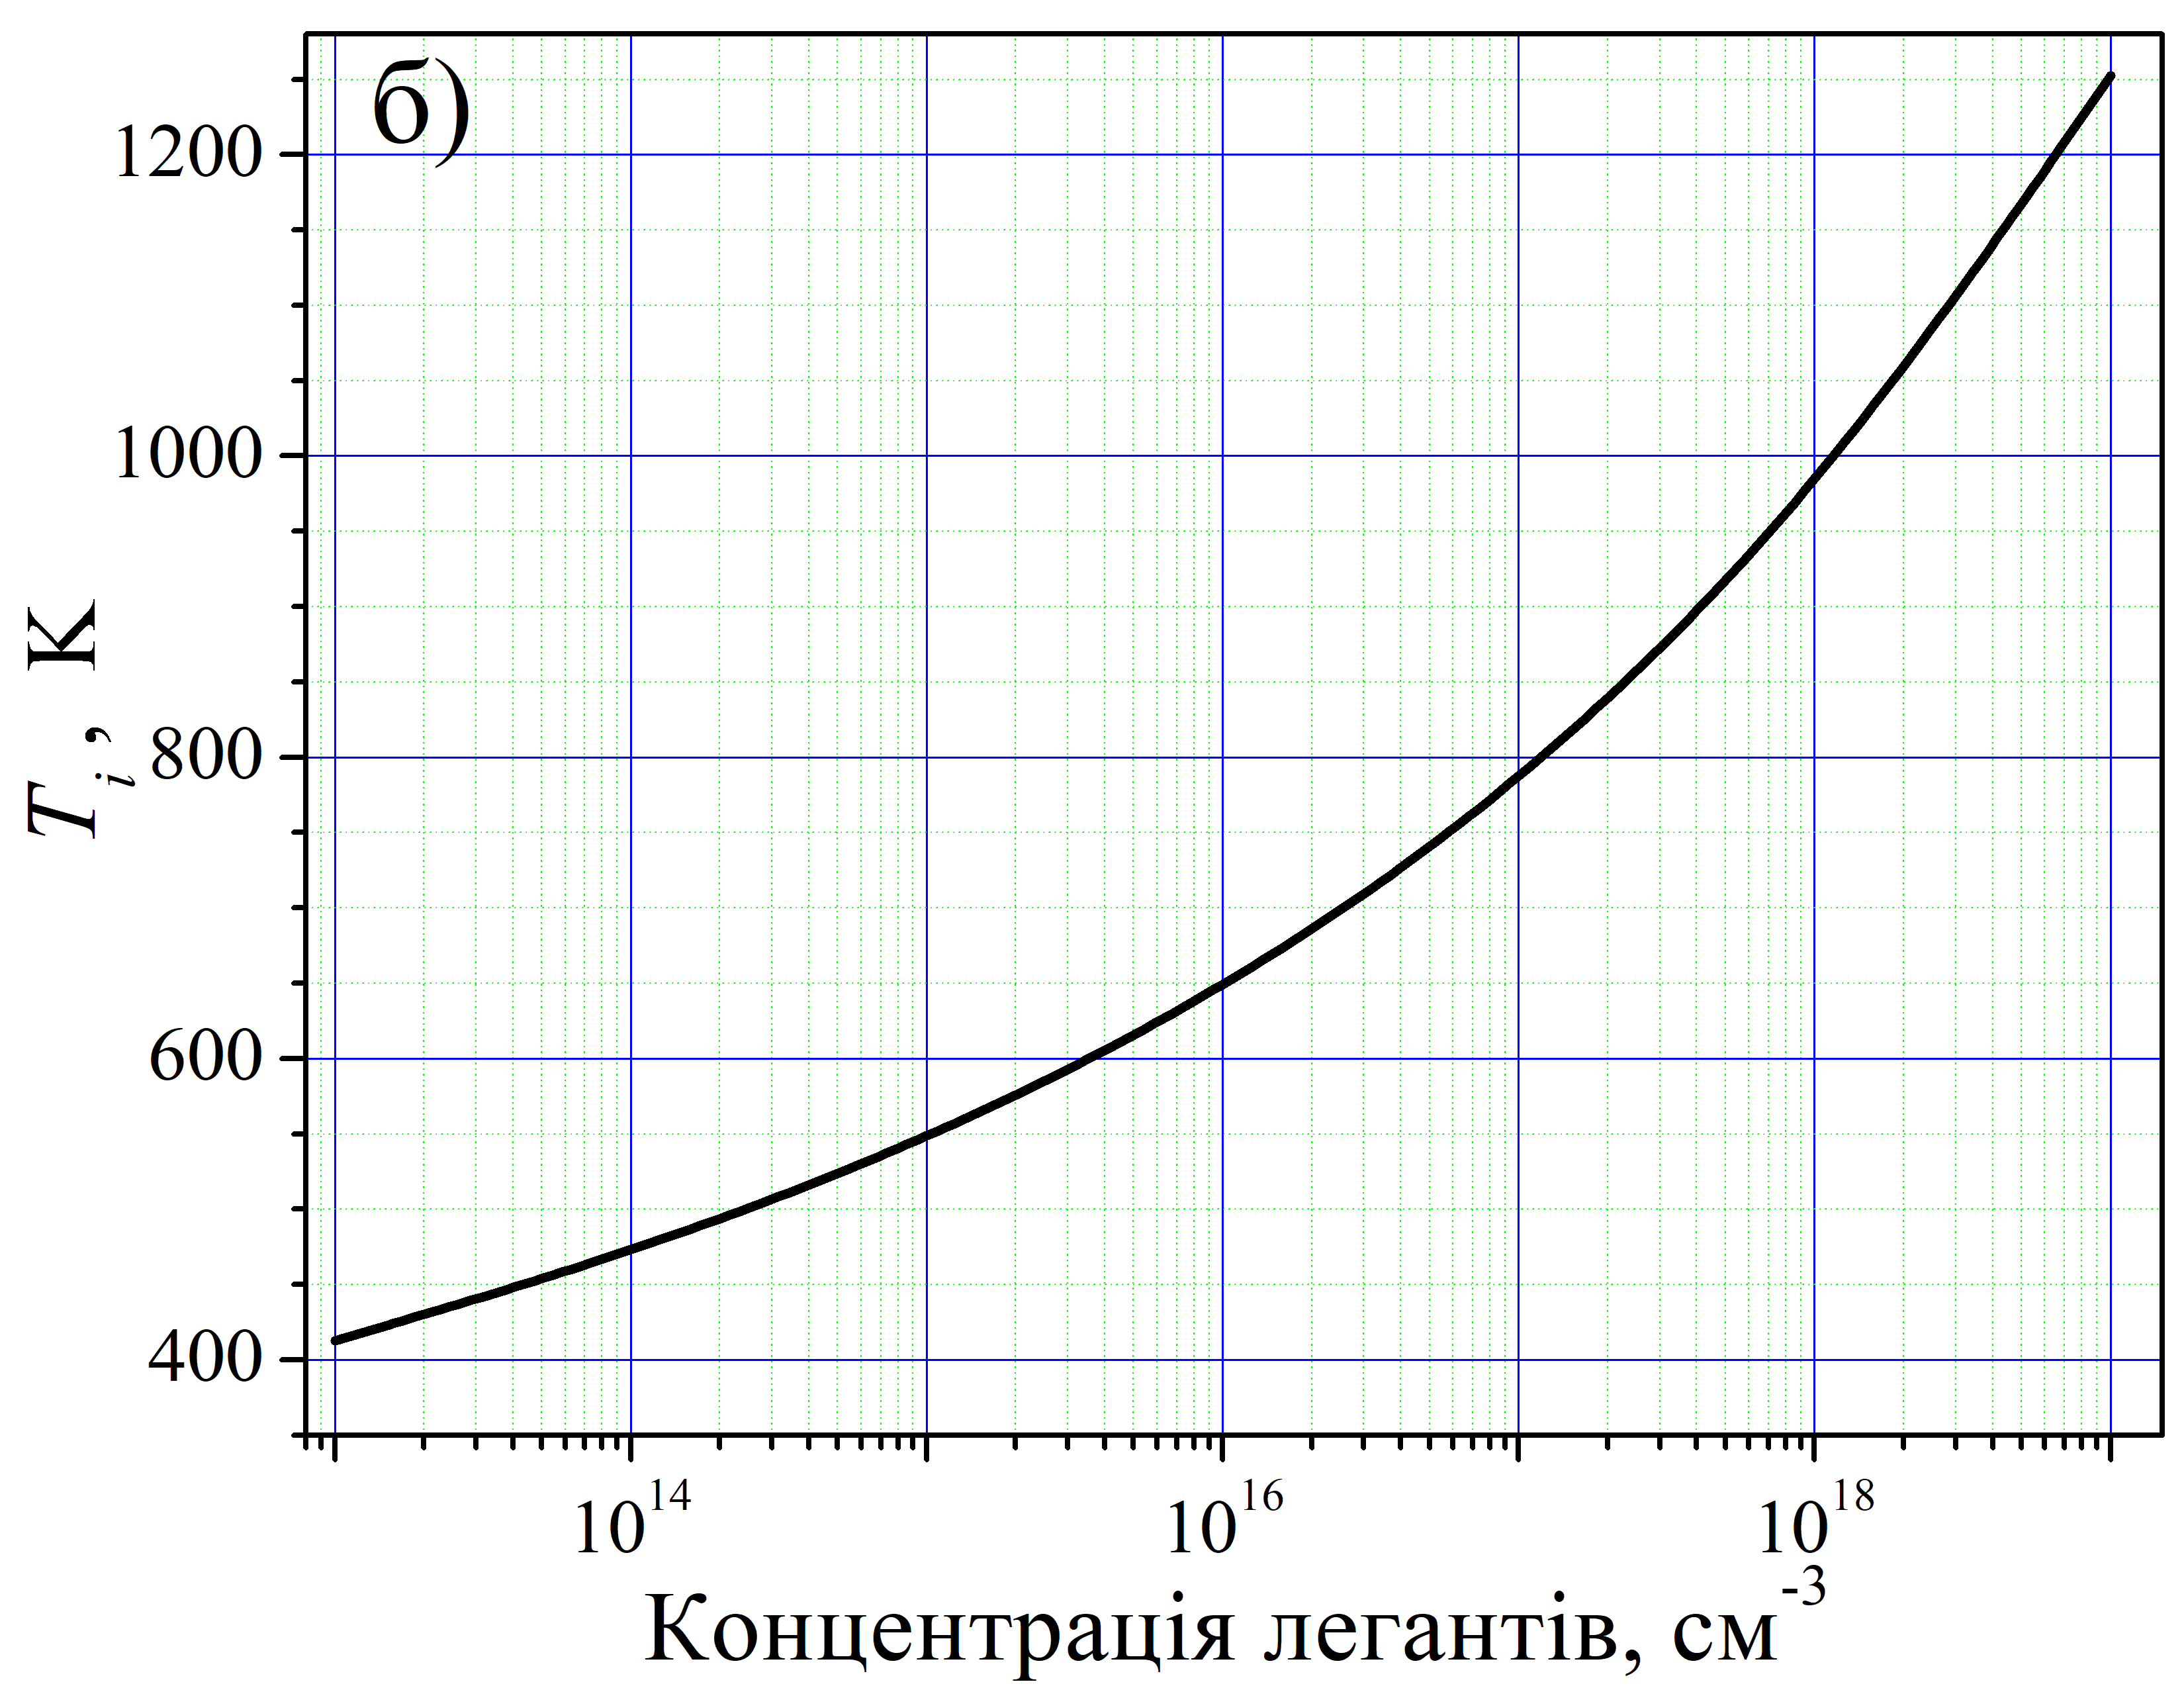
\includegraphics[width=0.49\linewidth]{FigTi.png}
	  \caption{Залежності виснаження (а) та температури початку власної провідності (б)
від концентрації легуючих домішок. У частині а наведено результати розрахунків для декількох типів легуючих домішок.
}\label{figTsTi}
\end{figure}

\section{Класичні регресійні моделі}

в Таблицях~\ref{tblRFrez}-\ref{tblDNNrez}.

\begin{table}
\setlength{\tabcolsep}{3pt}
\caption{Використані значення гіперпараметрів для RF моделей}
\label{tblRFrez}
\centering
\begin{tabular}{|l|c|c|c|c|c|c|c|c|}
\hline
Модель& \multicolumn{4}{c|}{RF\_N}& \multicolumn{4}{c|}{RF\_S} \rule{0pt}{11pt}\\
\hline
Цільова величина&$\mu_{n,n}$&$\mu_{n,p}$&$\mu_{p,p}$&$\mu_{p,n}$&$\mu_{n,n}$&$\mu_{n,p}$&$\mu_{p,p}$&$\mu_{p,n}$\\
\hline
Гіперпараметр&\multicolumn{8}{c|}{Значення}\\
\hline
\# estimators&468&500&658&510&278&564&304&204\\
\hline
max depth&19&58&37&19&30&15&55&55\\
\hline
min samples leaf &1&1&1&1&1&1&1&1\\
\hline
min samples split	&2&2&2&2&2&2&2&2\\
\hline
bootstrap	&True&True&True&True&True&True&True&True\\
\hline
max features &1,0&1,0&1,0&1,0&1,0&1,0&1,0&1,0\\
\hline
\end{tabular}
\end{table}


\begin{table}[!ht]
\setlength{\tabcolsep}{3pt}
\caption{Використані значення гіперпараметрів для GB моделей}
\label{tblGBrez}
\centering
\begin{tabular}{|l|c|c|c|c|c|c|c|c|}
\hline
Модель& \multicolumn{4}{c|}{GB\_N}& \multicolumn{4}{c|}{GB\_S} \rule{0pt}{11pt}\\
\hline
Цільова величина&$\mu_{n,n}$&$\mu_{n,p}$&$\mu_{p,p}$&$\mu_{p,n}$&$\mu_{n,n}$&$\mu_{n,p}$&$\mu_{p,p}$&$\mu_{p,n}$\\
\hline
Гіперпараметр&\multicolumn{8}{c|}{Значення}\\
\hline
\# estimators&700&800&800&570&840&770&810&850\\
\hline
max depth&4&4&4&4&4&4&2&4\\
\hline
min samples leaf &6&2&5&4&5&3&5&4\\
\hline
min samples split	&2&2&3&3&5&5&5&6\\
\hline
learning rate, $10^{-2}$	&6,44&9,78&7,69&4,68&9,49&4,63&9,67&5,29\\
\hline
max features &0,8&1,0&1,0&0,6&1,0&0,7&1,0&0,8\\
\hline
\end{tabular}
\end{table}

\begin{table}[!ht]
\setlength{\tabcolsep}{3pt}
\caption{Використані значення гіперпараметрів для SVR моделей}
\label{tblSVRrez}
\centering
\begin{tabular}{|l|c|c|c|c|c|c|c|c|}
\hline
Модель& \multicolumn{4}{c|}{SVR\_N}& \multicolumn{4}{c|}{SVP\_S} \rule{0pt}{11pt}\\
\hline
Цільова величина&$\mu_{n,n}$&$\mu_{n,p}$&$\mu_{p,p}$&$\mu_{p,n}$&$\mu_{n,n}$&$\mu_{n,p}$&$\mu_{p,p}$&$\mu_{p,n}$\\
\hline
Гіперпараметр&\multicolumn{8}{c|}{Значення}\\
\hline
kernel &poly&poly&poly&poly&rbf&rbf&rbf&rbf\\
\hline
degree&6&6&6&6&--&--&--&--\\
\hline
$C_0$ &7,52&7,54&7,08&7,02&4,92&2,73&3,88&6,78\\
\hline
Tolerance, $10^{-3}$&5,64&2,22&0,60&0,015&0,75&0,32&0,083&0,068\\
\hline
$C$	&9,79&7,04&3,00&4,19&15&15&15&15\\
\hline
$\varepsilon$, $10^{-3}$ &33,2&11,6&10,4&0,91&0,55&0,50&2,44&0,84\\
\hline
\end{tabular}
\end{table}

\begin{table}[!ht]
\setlength{\tabcolsep}{1pt}
\caption{Використані значення гіперпараметрів для DNN моделей}
\label{tblDNNrez}
\centering
\begin{tabular}{|l|c|c|c|c|c|c|c|c|}
\hline
Модель& \multicolumn{4}{c|}{DNN\_N}& \multicolumn{4}{c|}{DNN\_S} \rule{0pt}{11pt}\\
\hline
Цільова величина&$\mu_{n,n}$&$\mu_{n,p}$&$\mu_{p,p}$&$\mu_{p,n}$&$\mu_{n,n}$&$\mu_{n,p}$&$\mu_{p,p}$&$\mu_{p,n}$\\
\hline
Гіперпараметр&\multicolumn{8}{c|}{Значення}\\
\hline
\makecell{\# nodes for first \\hidden layer} &25&100&25&75&25&75&100&25\\
\hline
batch size&\multicolumn{8}{c|}{16}\\
\hline
activation function &\multicolumn{2}{c|}{SELU}&ReLu&SELU&sigmoid&ReLu&\multicolumn{2}{c|}{sigmoid}\\
\hline
optimizer	&Nadam&\multicolumn{4}{c|}{Adamax}&Nadam&\multicolumn{2}{c|}{Adamax}\\
\hline
learning rate, $10^{-3}$	&0,58&1,25&8,05&5,17&13,0&4,89&12,8&2,84\\
\hline
%weight initializer &\makecell{Xavier \\Normal}&\multicolumn{2}{c|}{He Normal}&\makecell{Xavier \\Normal}&\multicolumn{3}{c|}{He Normal}&\makecell{Xavier \\Normal}\\
weight initializer &Xavier Normal&\multicolumn{2}{c|}{He Normal}&Xavier Normal&\multicolumn{3}{c|}{He Normal}&Xavier Normal\\
\hline
\# epoch &\multicolumn{8}{c|}{1000}\\
\hline
\end{tabular}
\end{table}

\begin{figure}
	\centering
     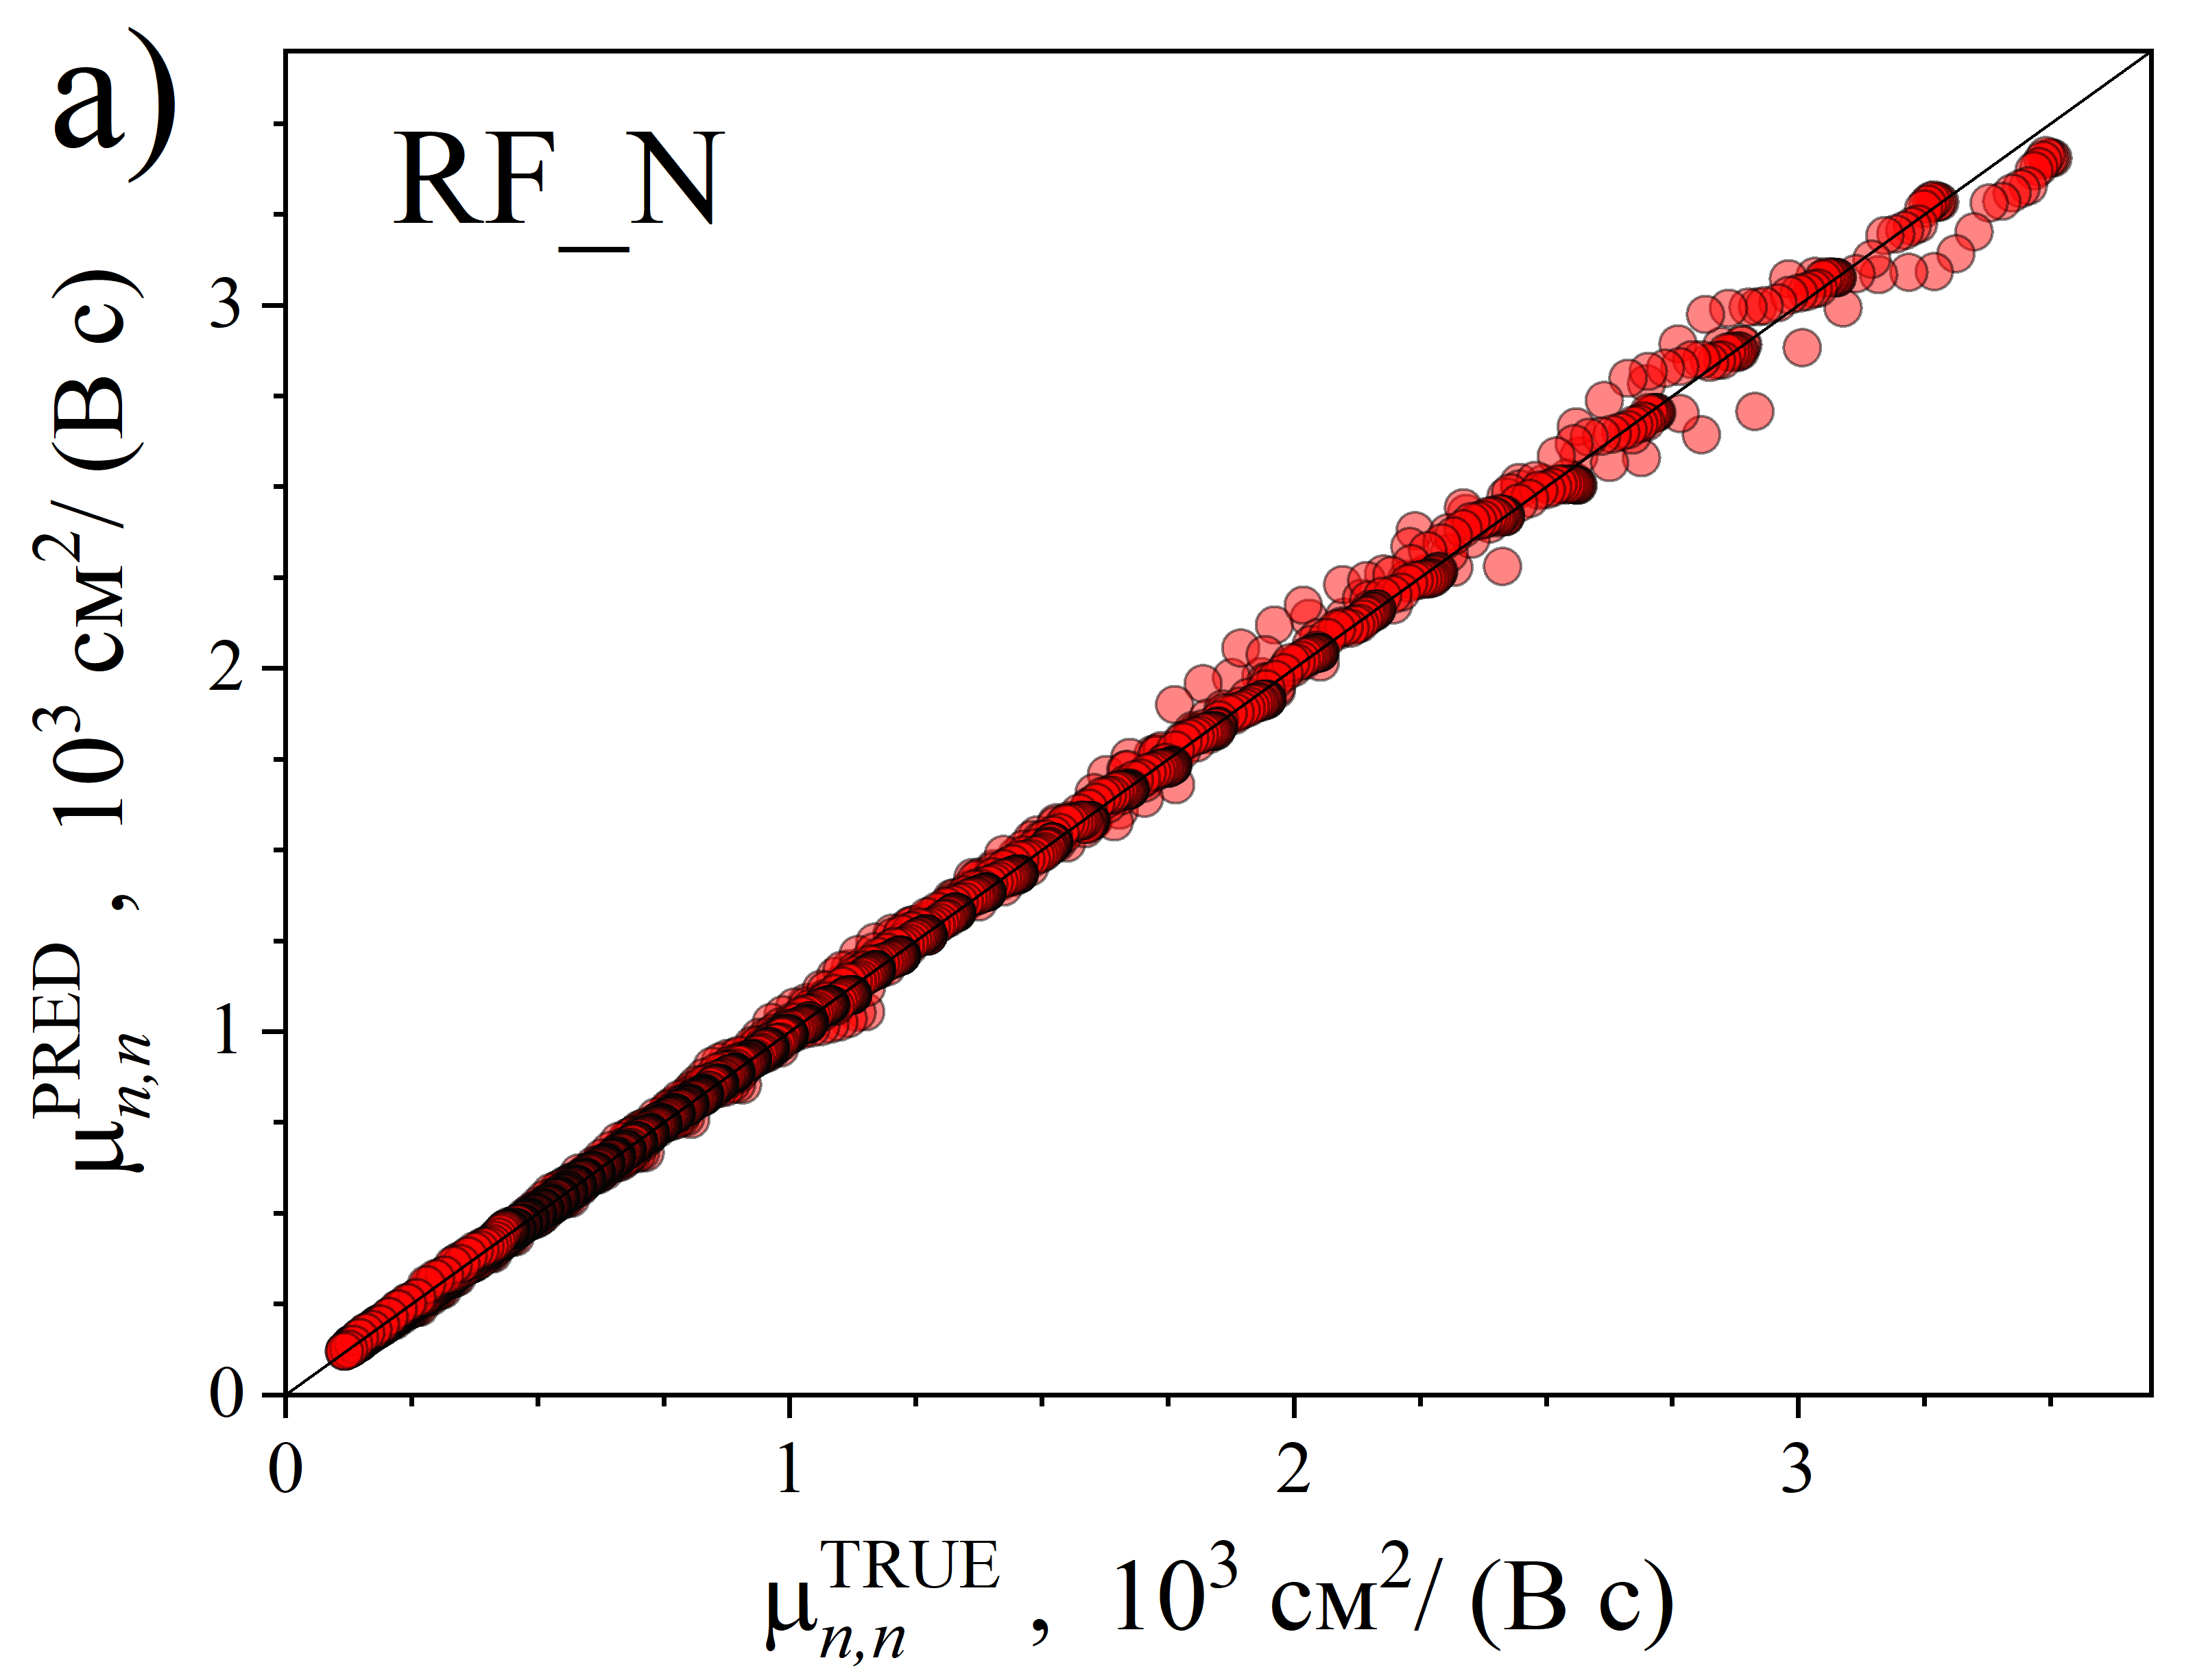
\includegraphics[width=0.35\linewidth]{RFNnn.png}\kern 20pt
     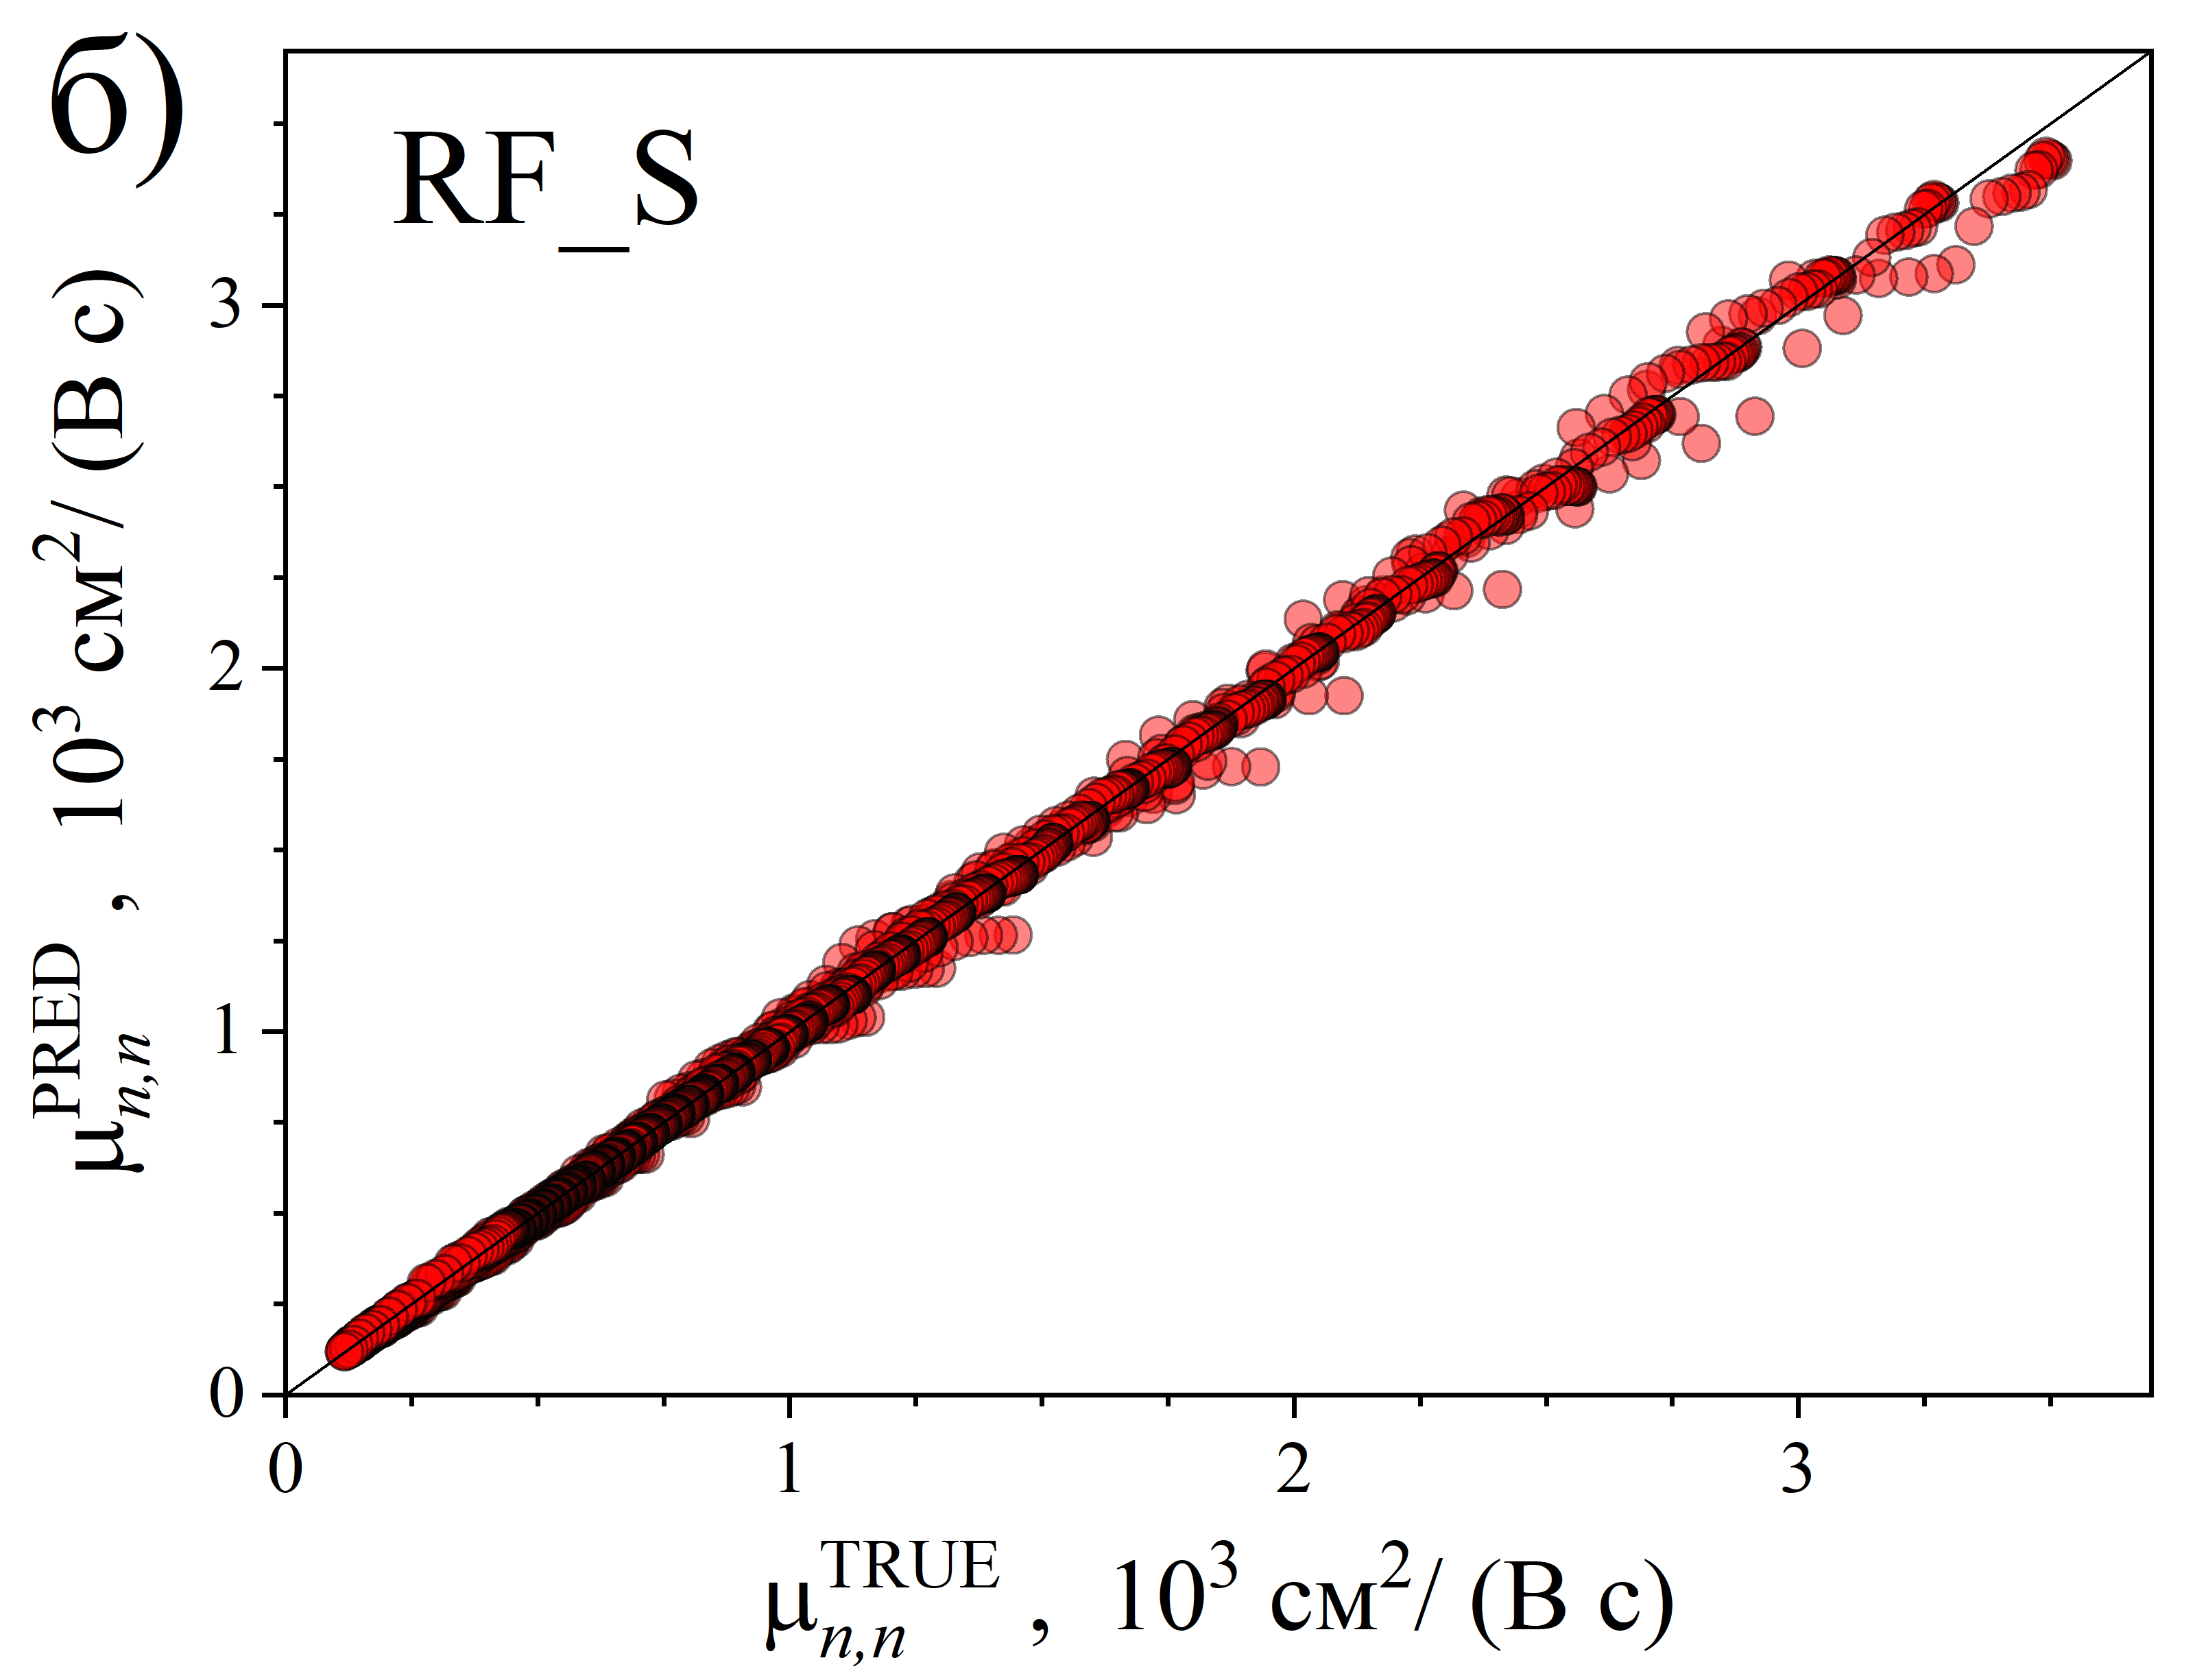
\includegraphics[width=0.35\linewidth]{RFSnn.png}
     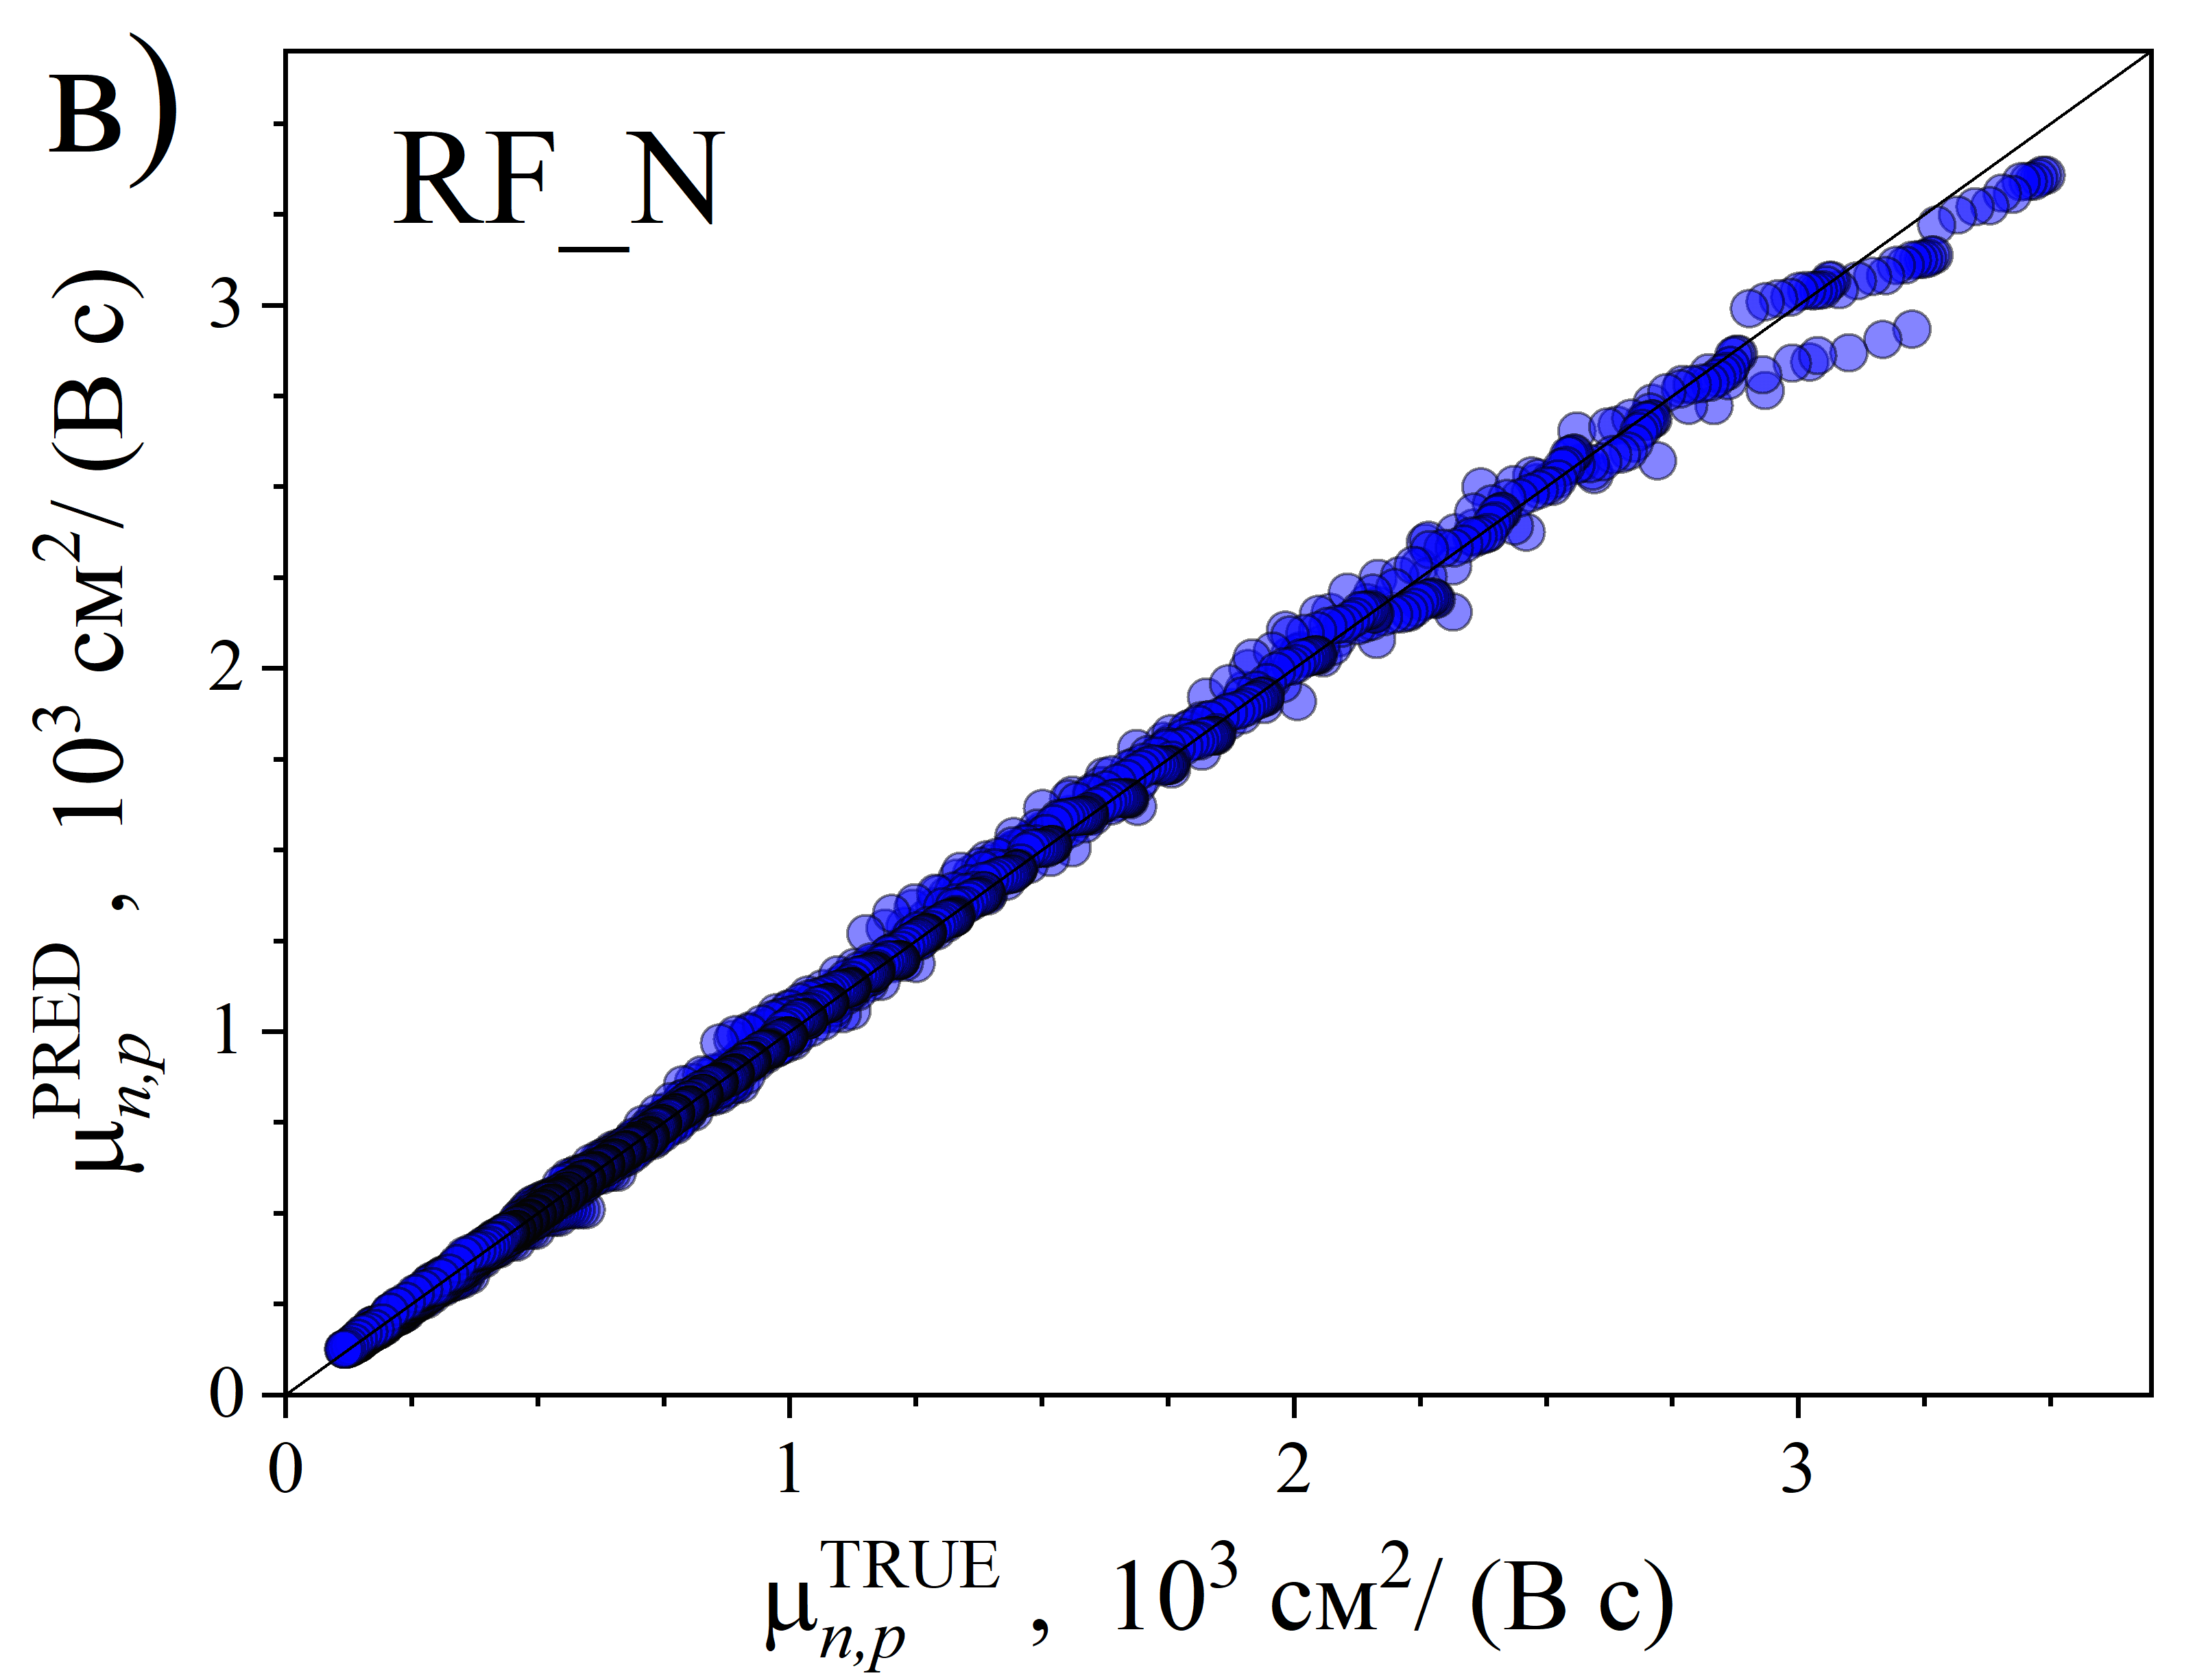
\includegraphics[width=0.35\linewidth]{RFNnp.png}\kern 20pt
     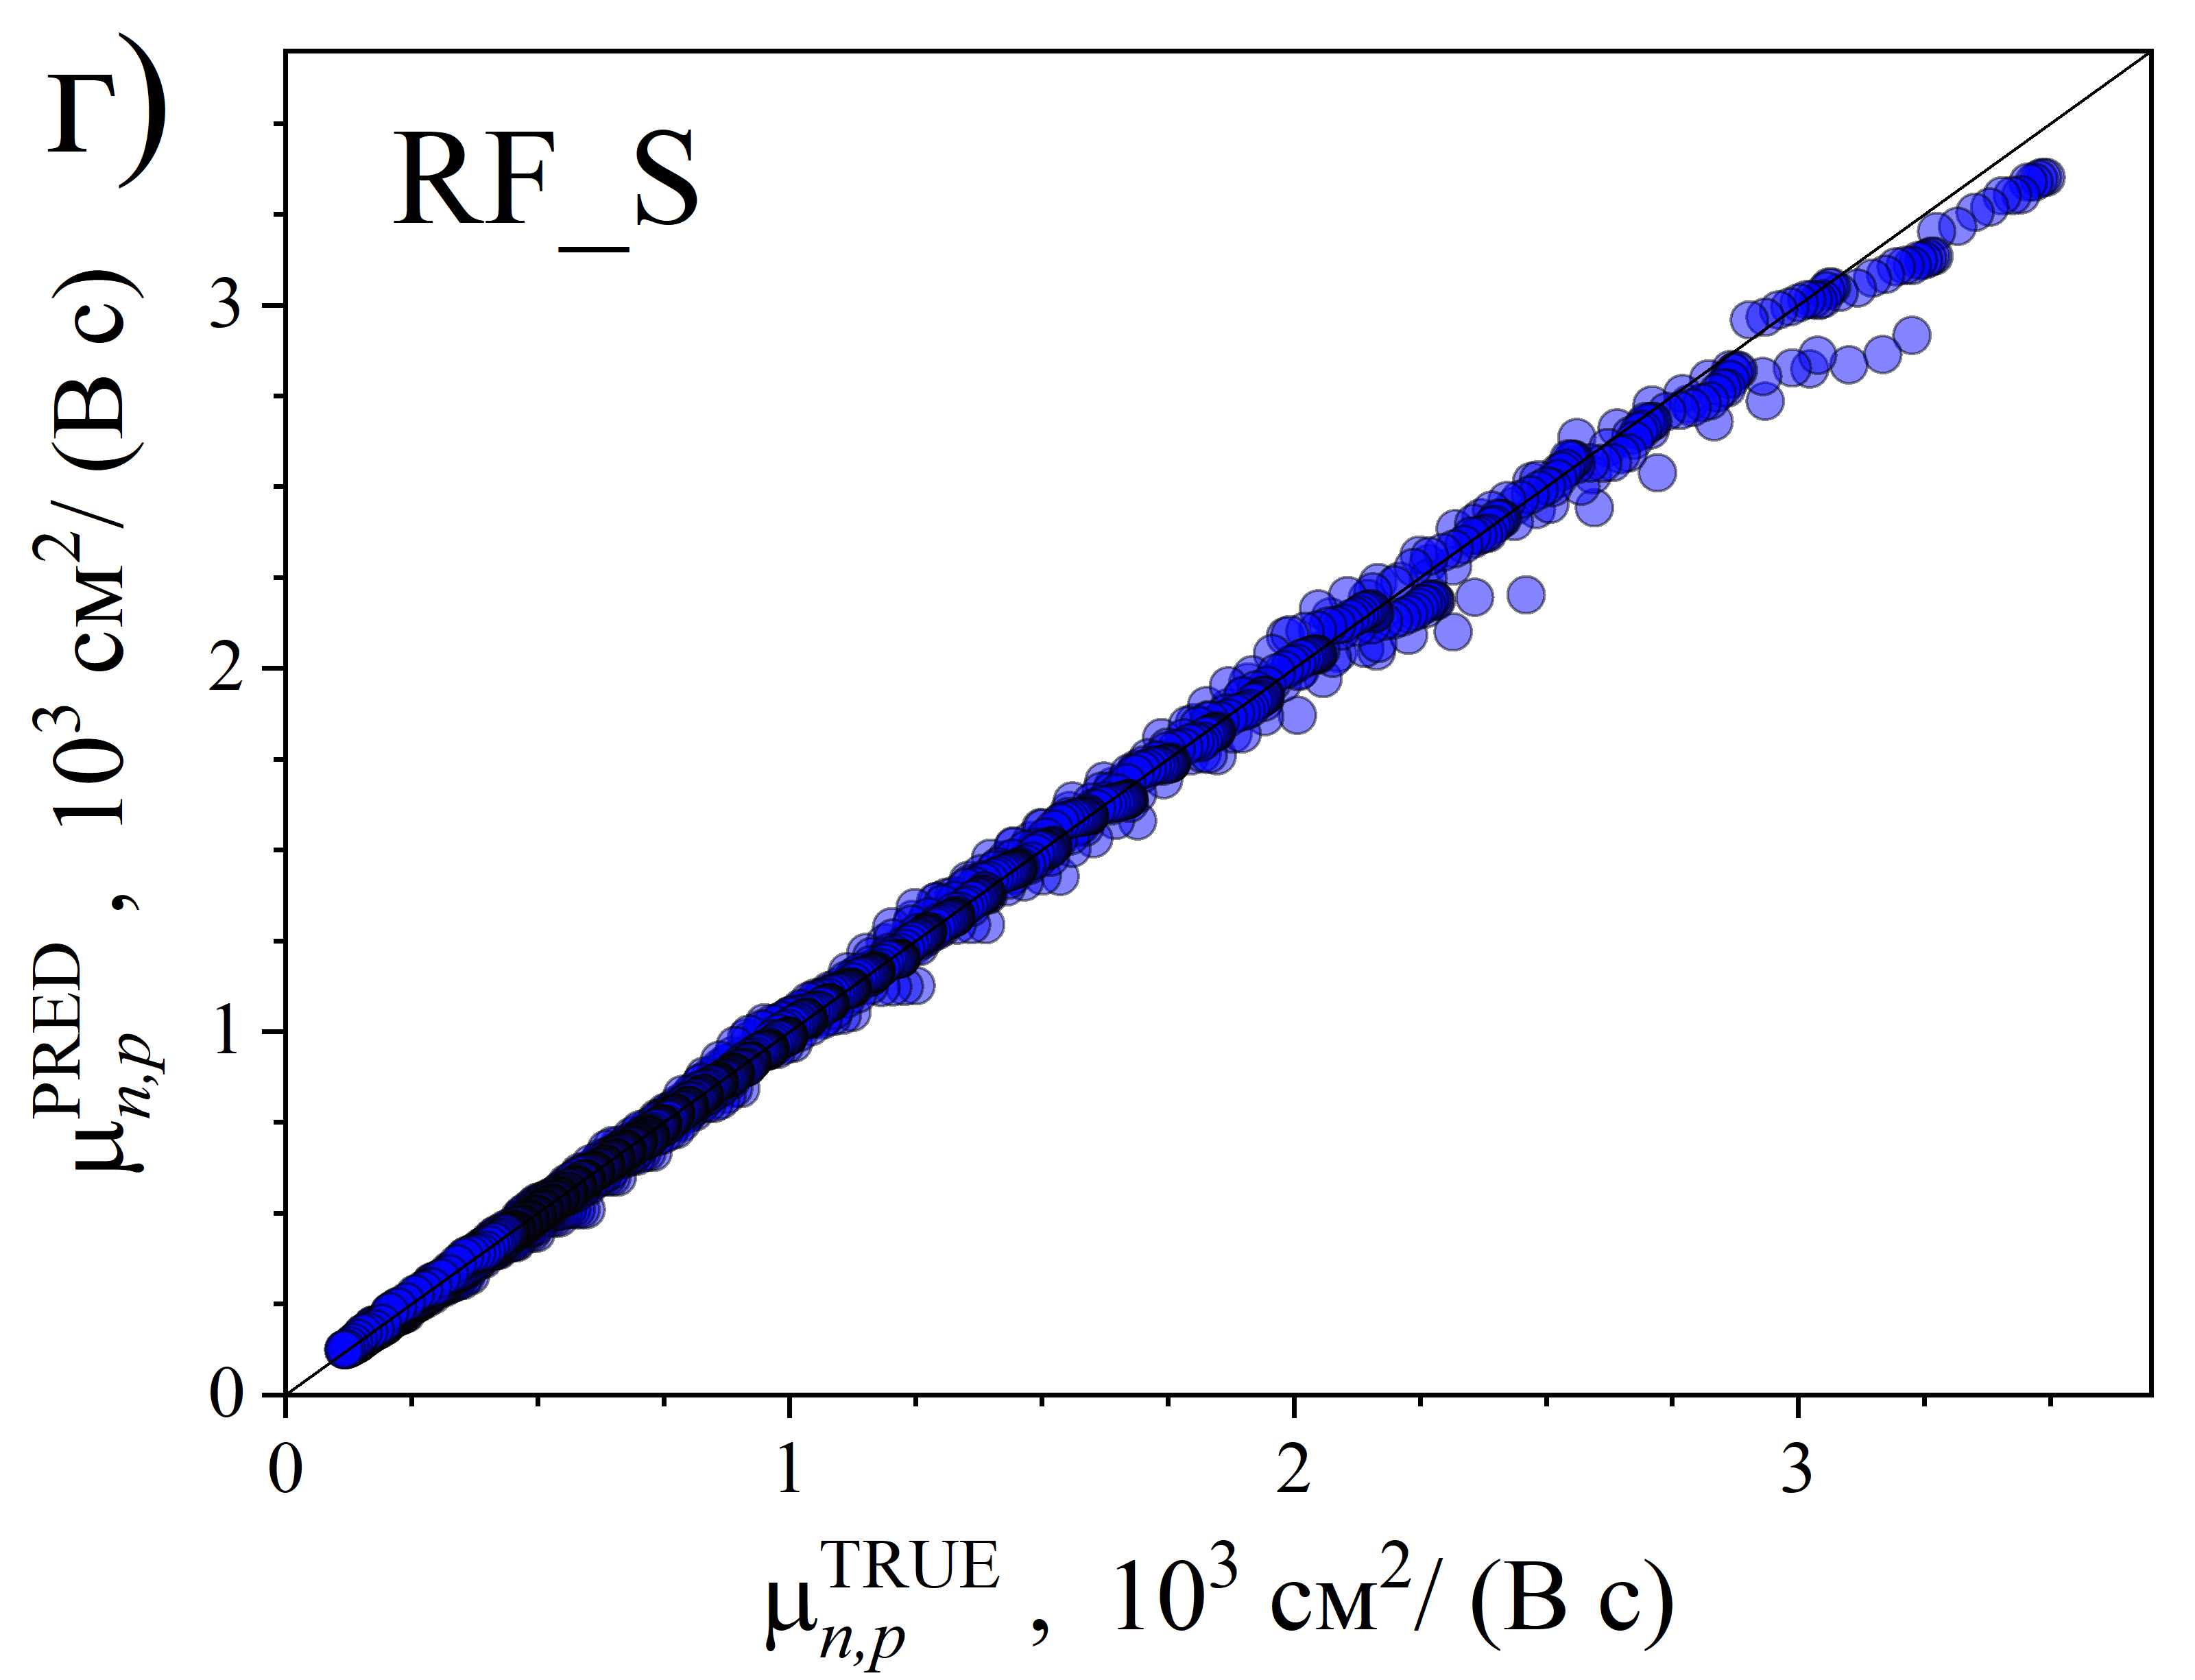
\includegraphics[width=0.35\linewidth]{RFSnp.png}
     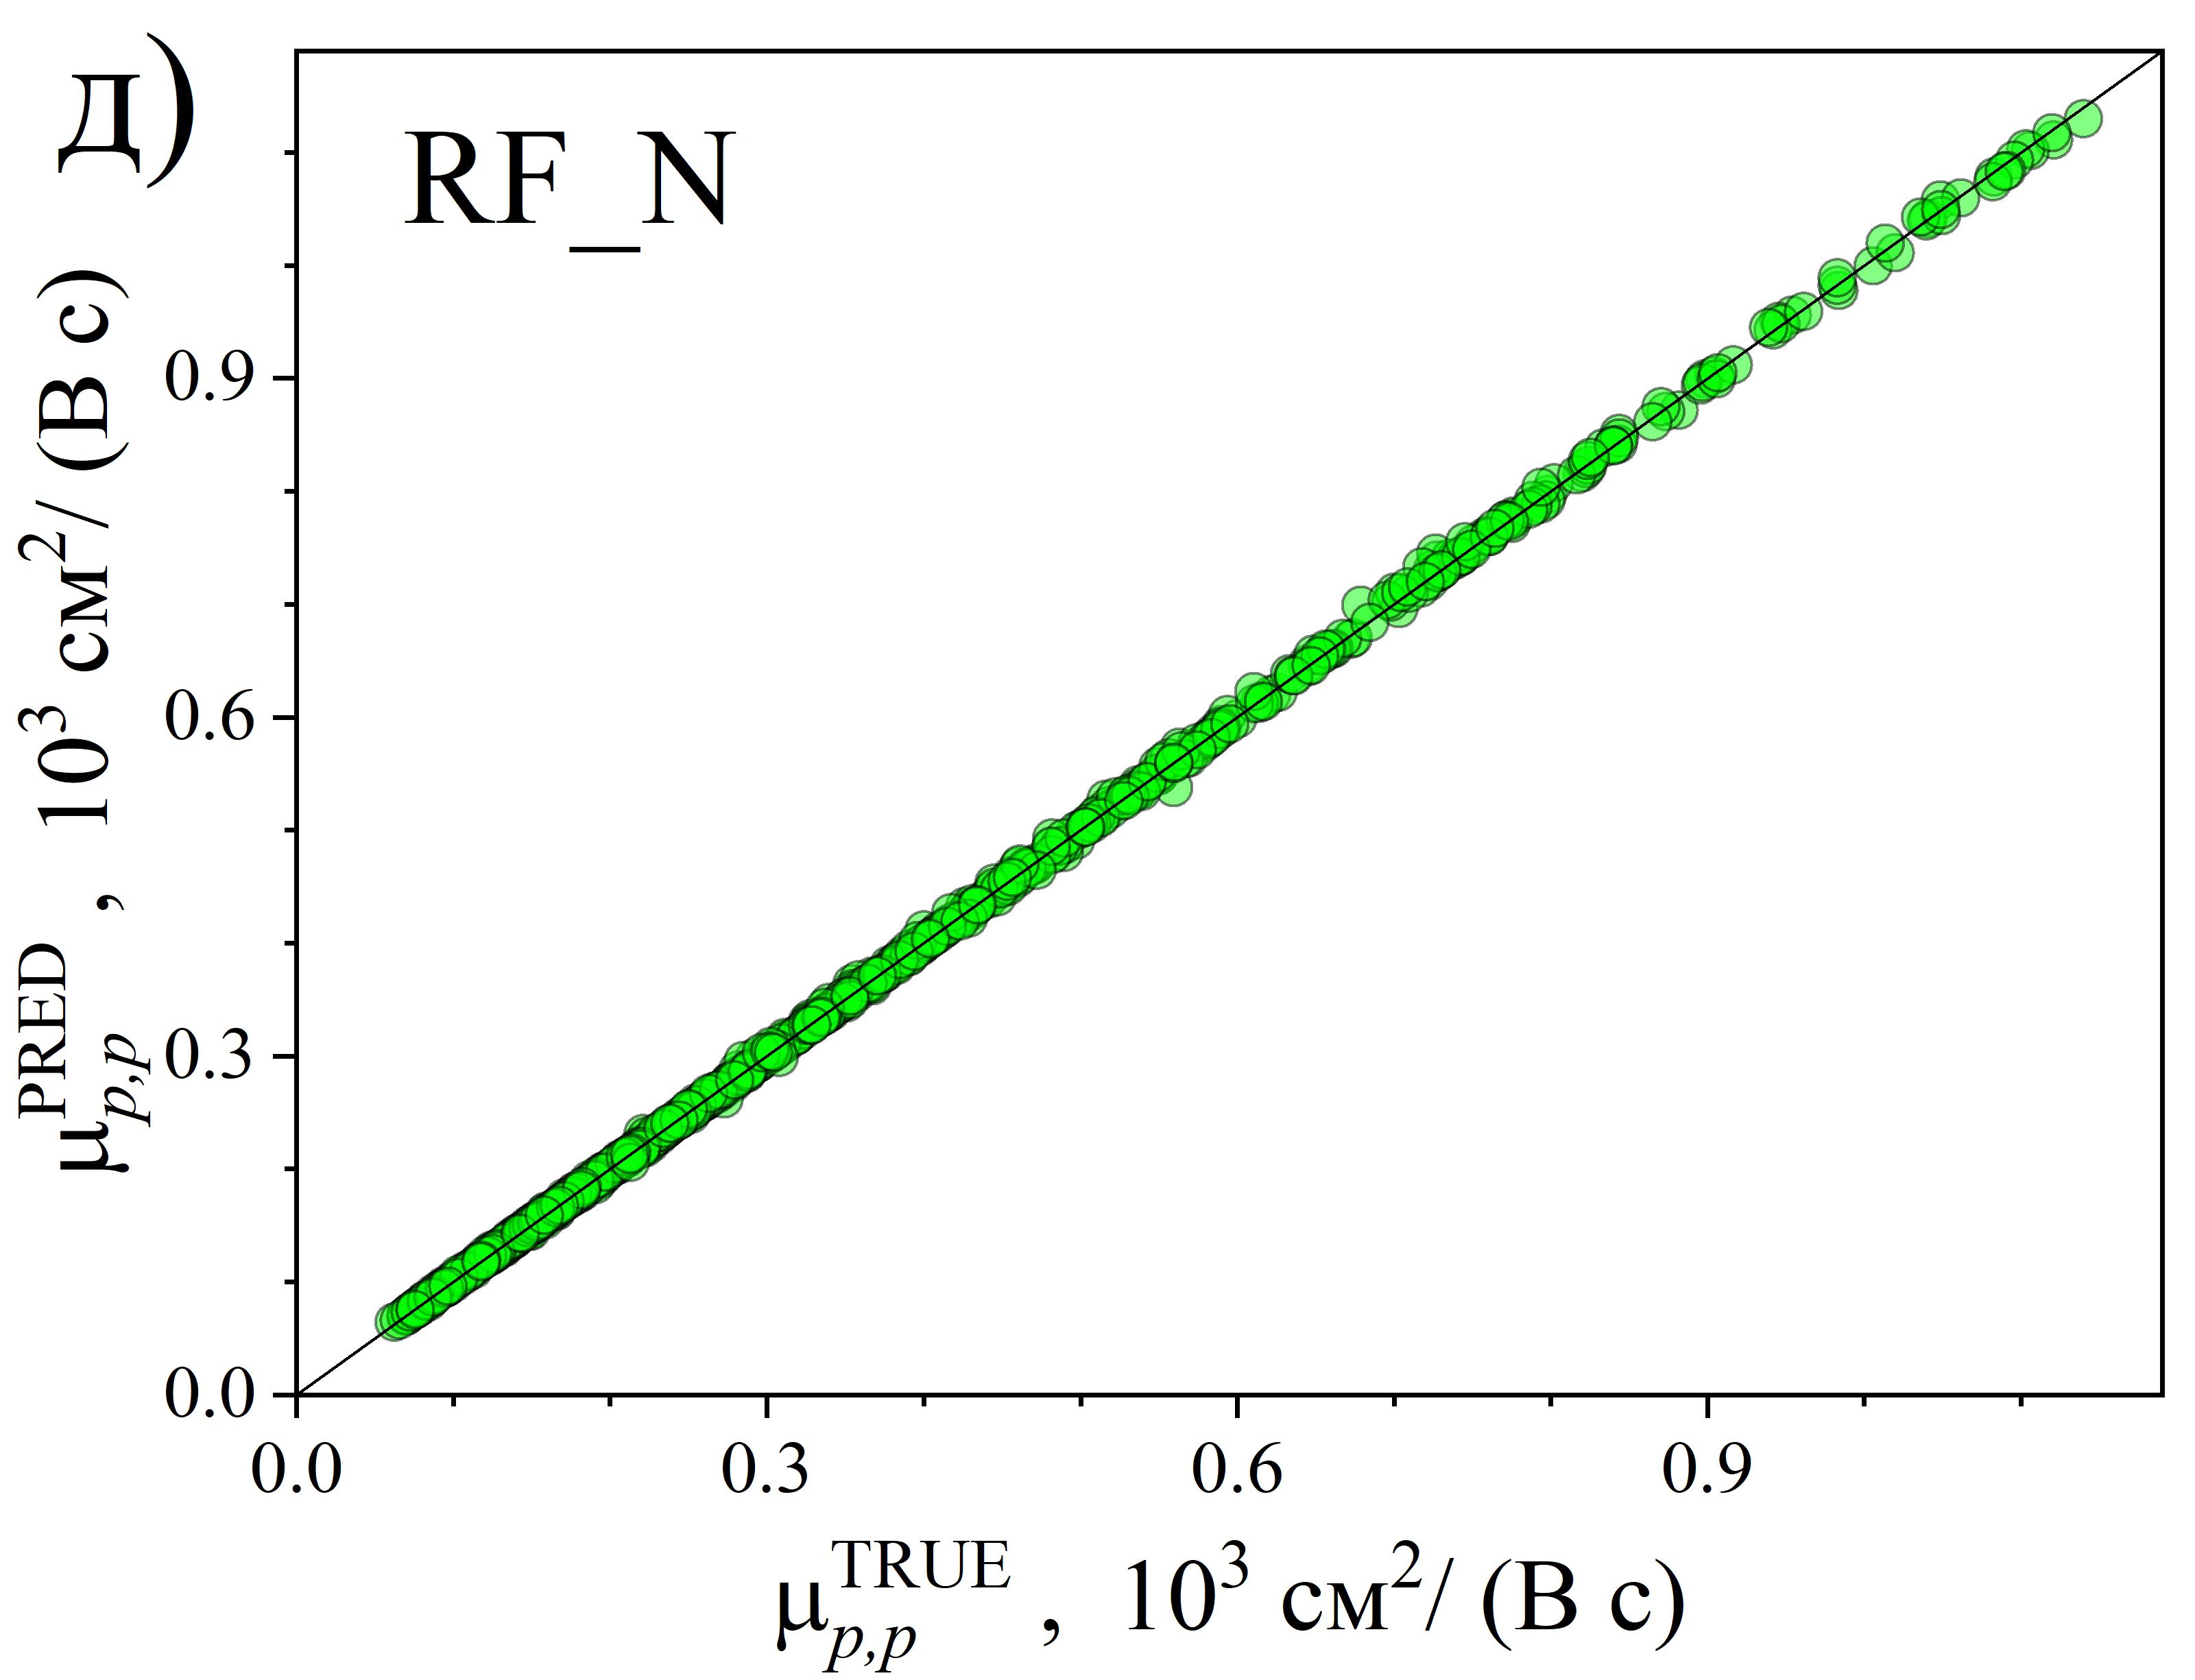
\includegraphics[width=0.35\linewidth]{RFNpp.png}\kern 20pt
     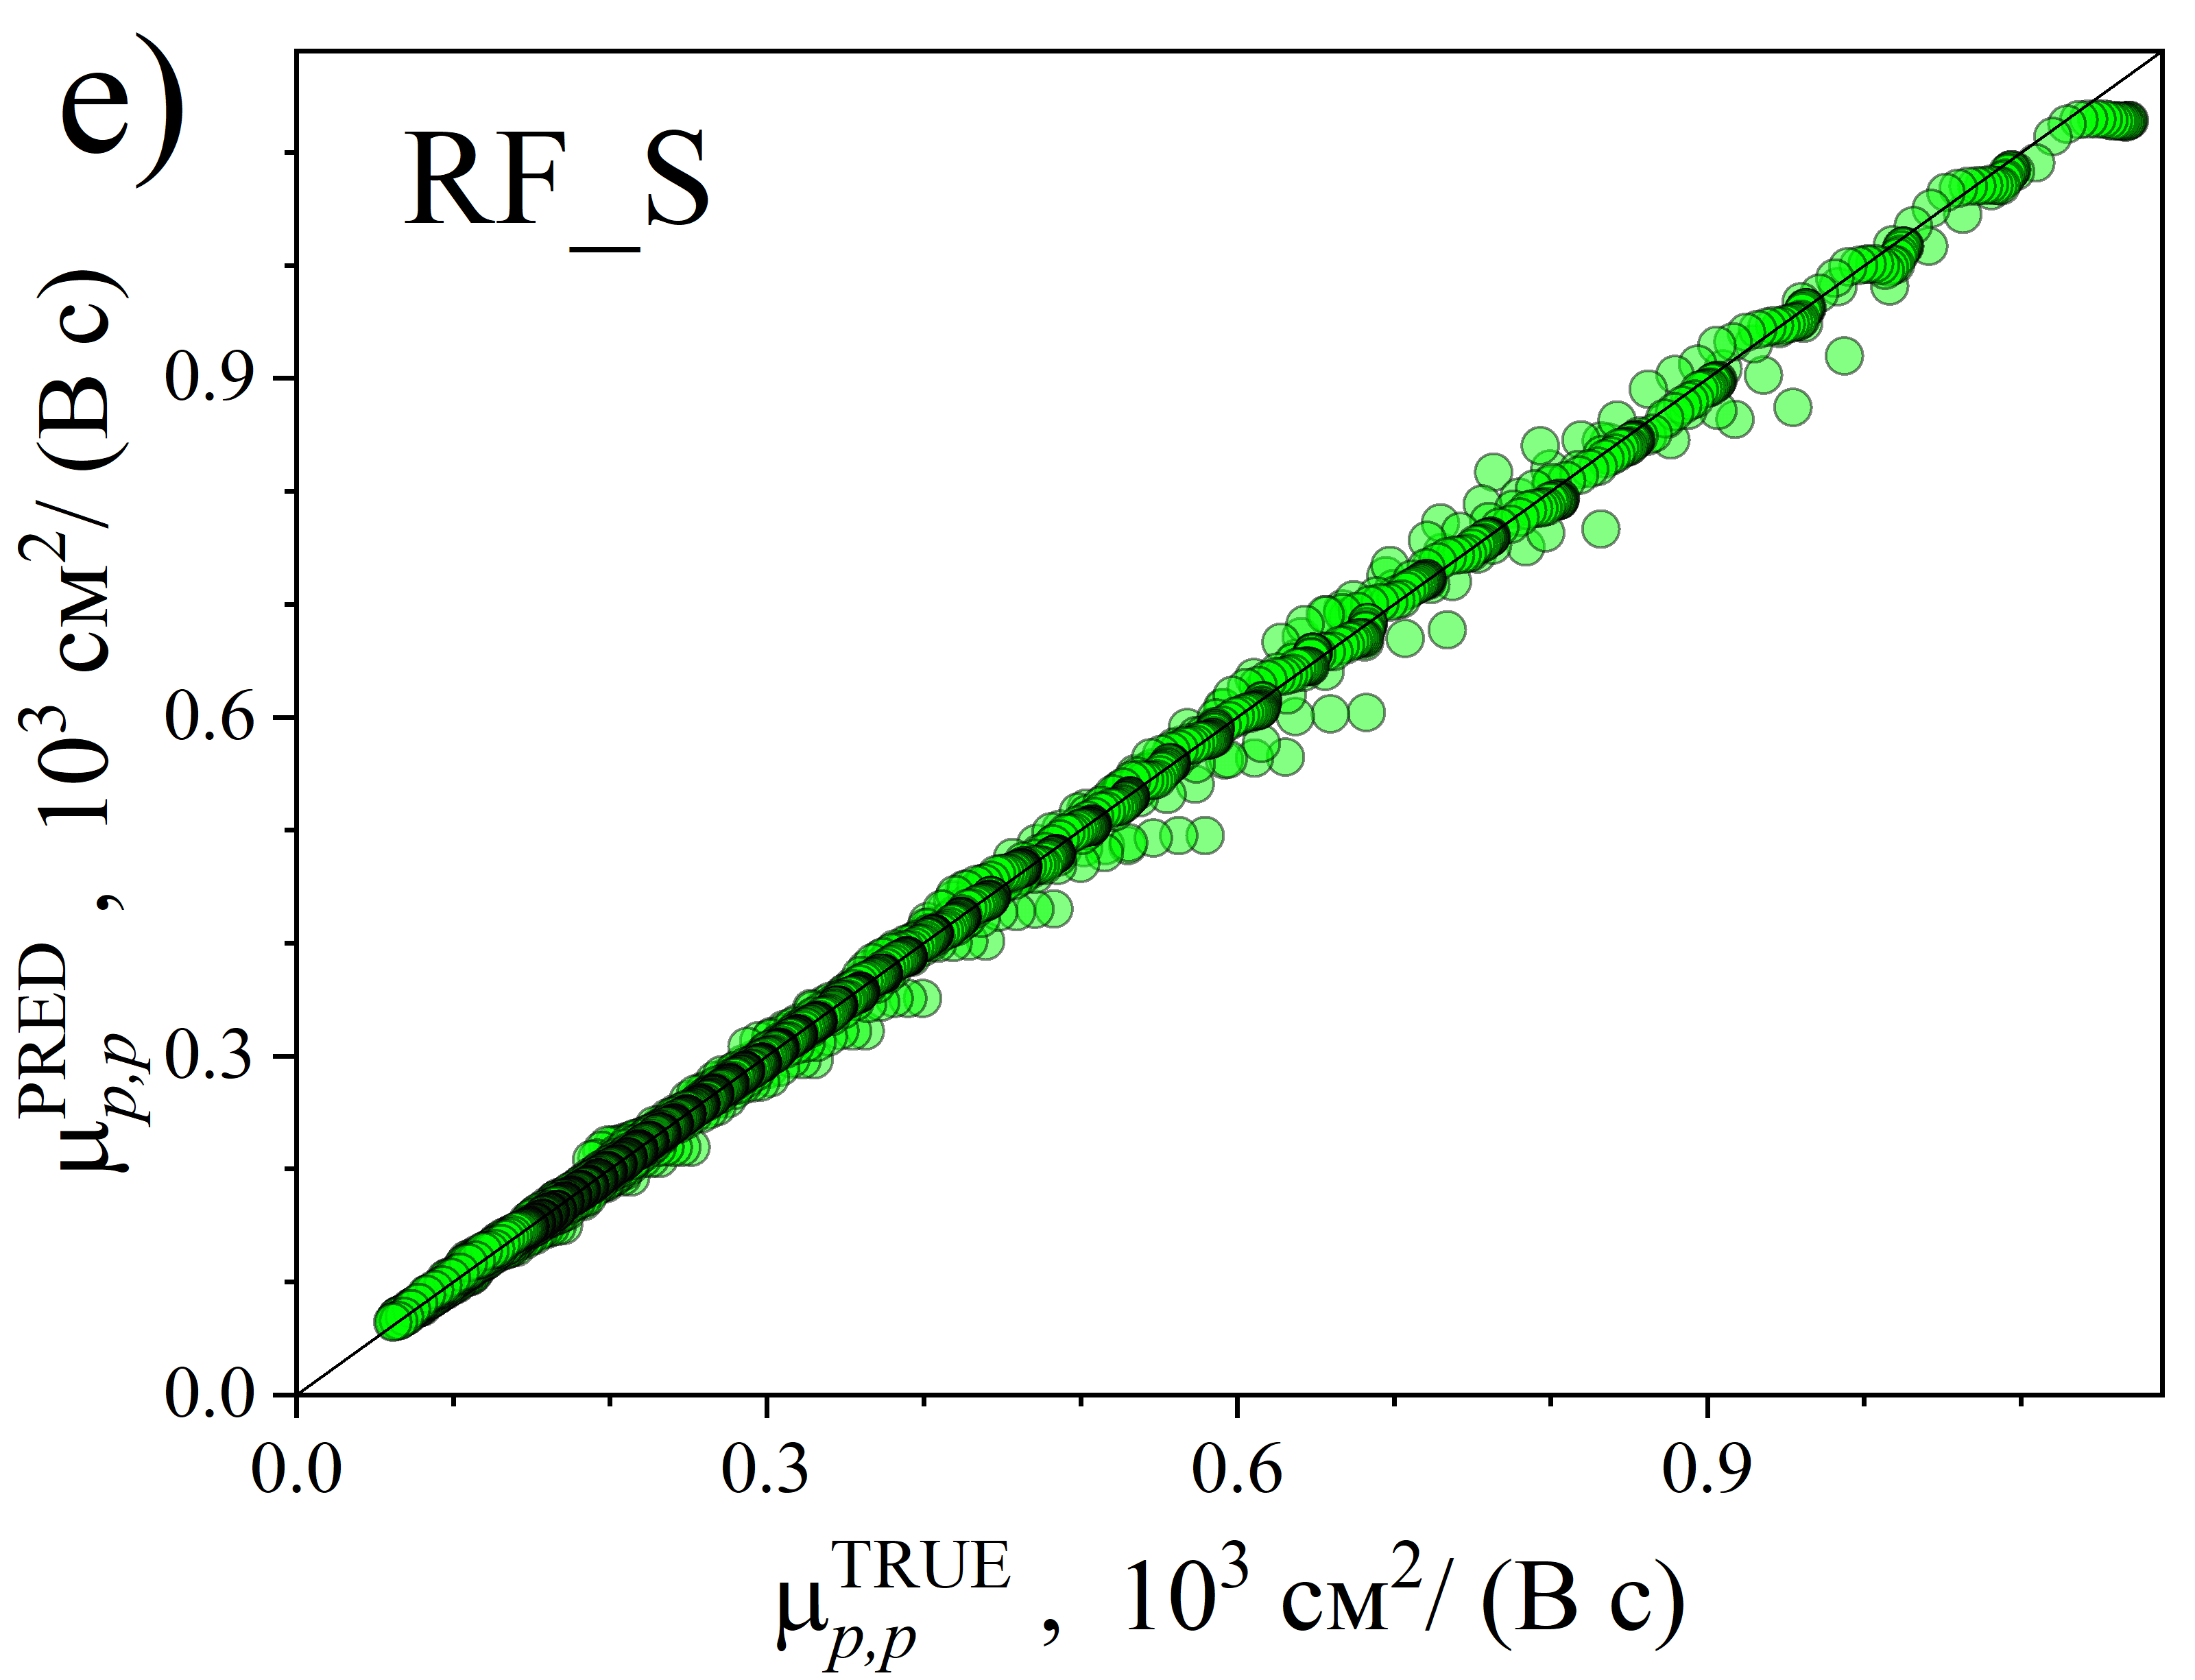
\includegraphics[width=0.35\linewidth]{RFSpp.png}
     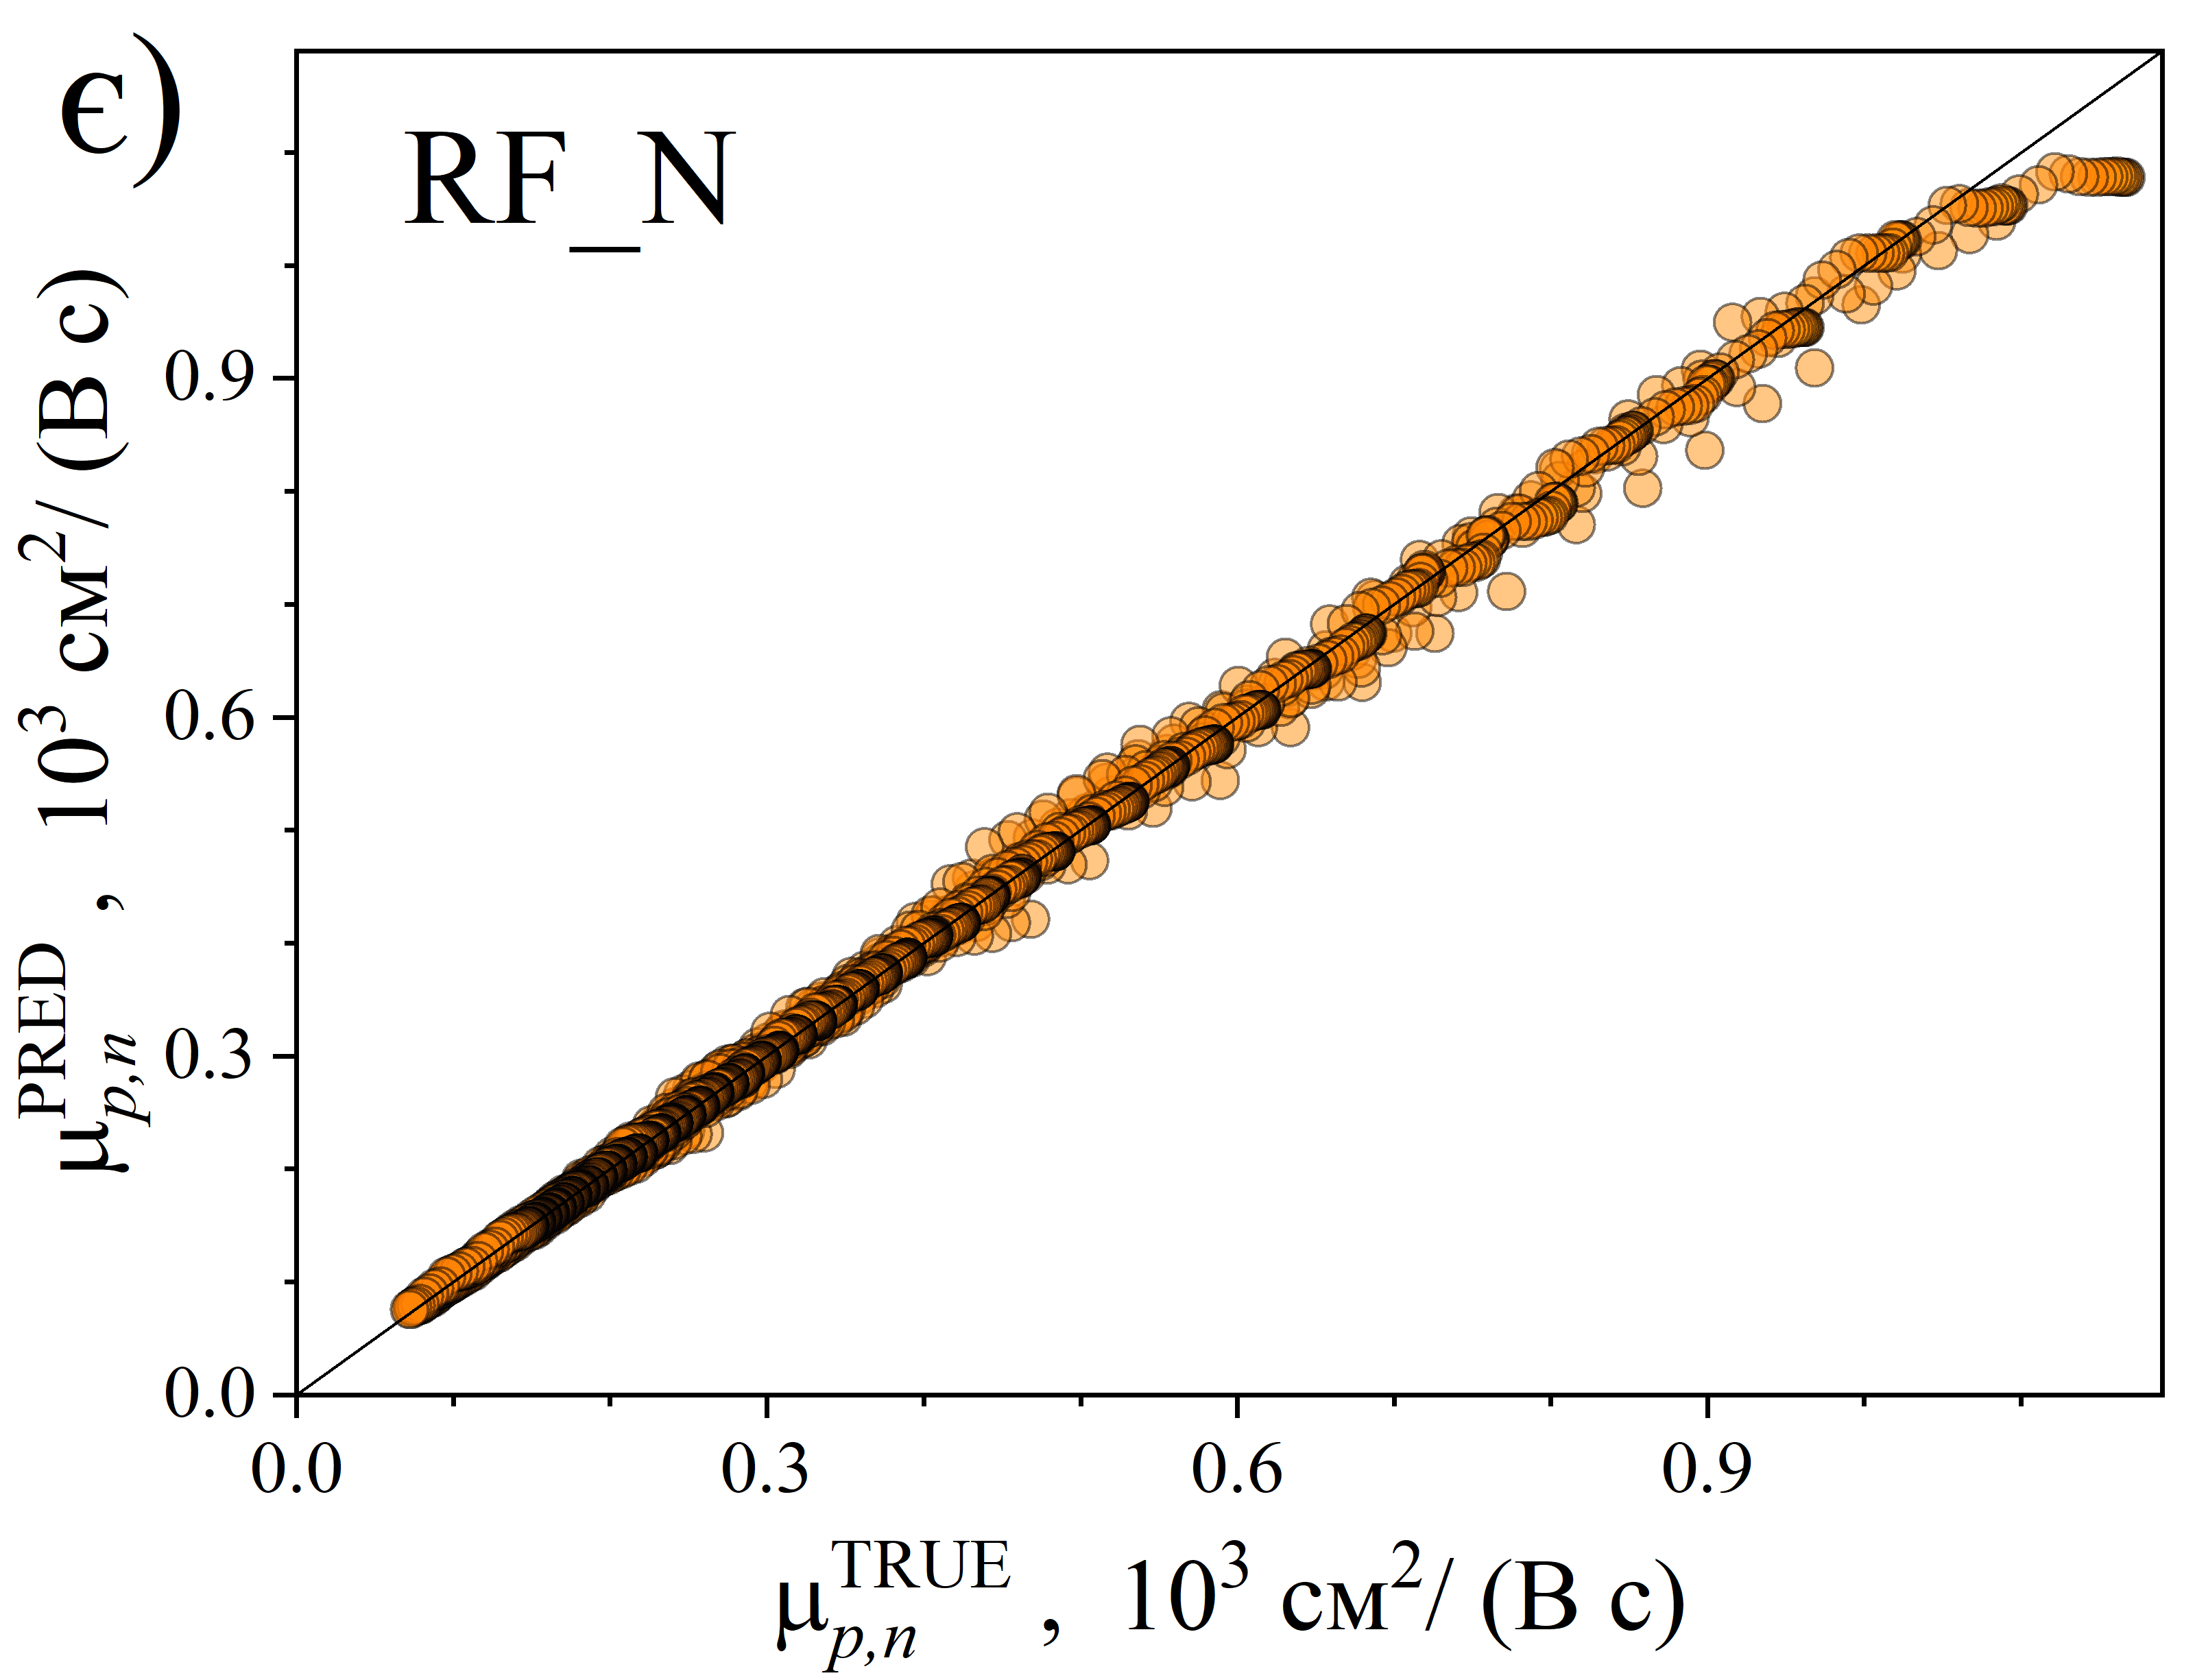
\includegraphics[width=0.35\linewidth]{RFNpn.png}\kern 20pt
     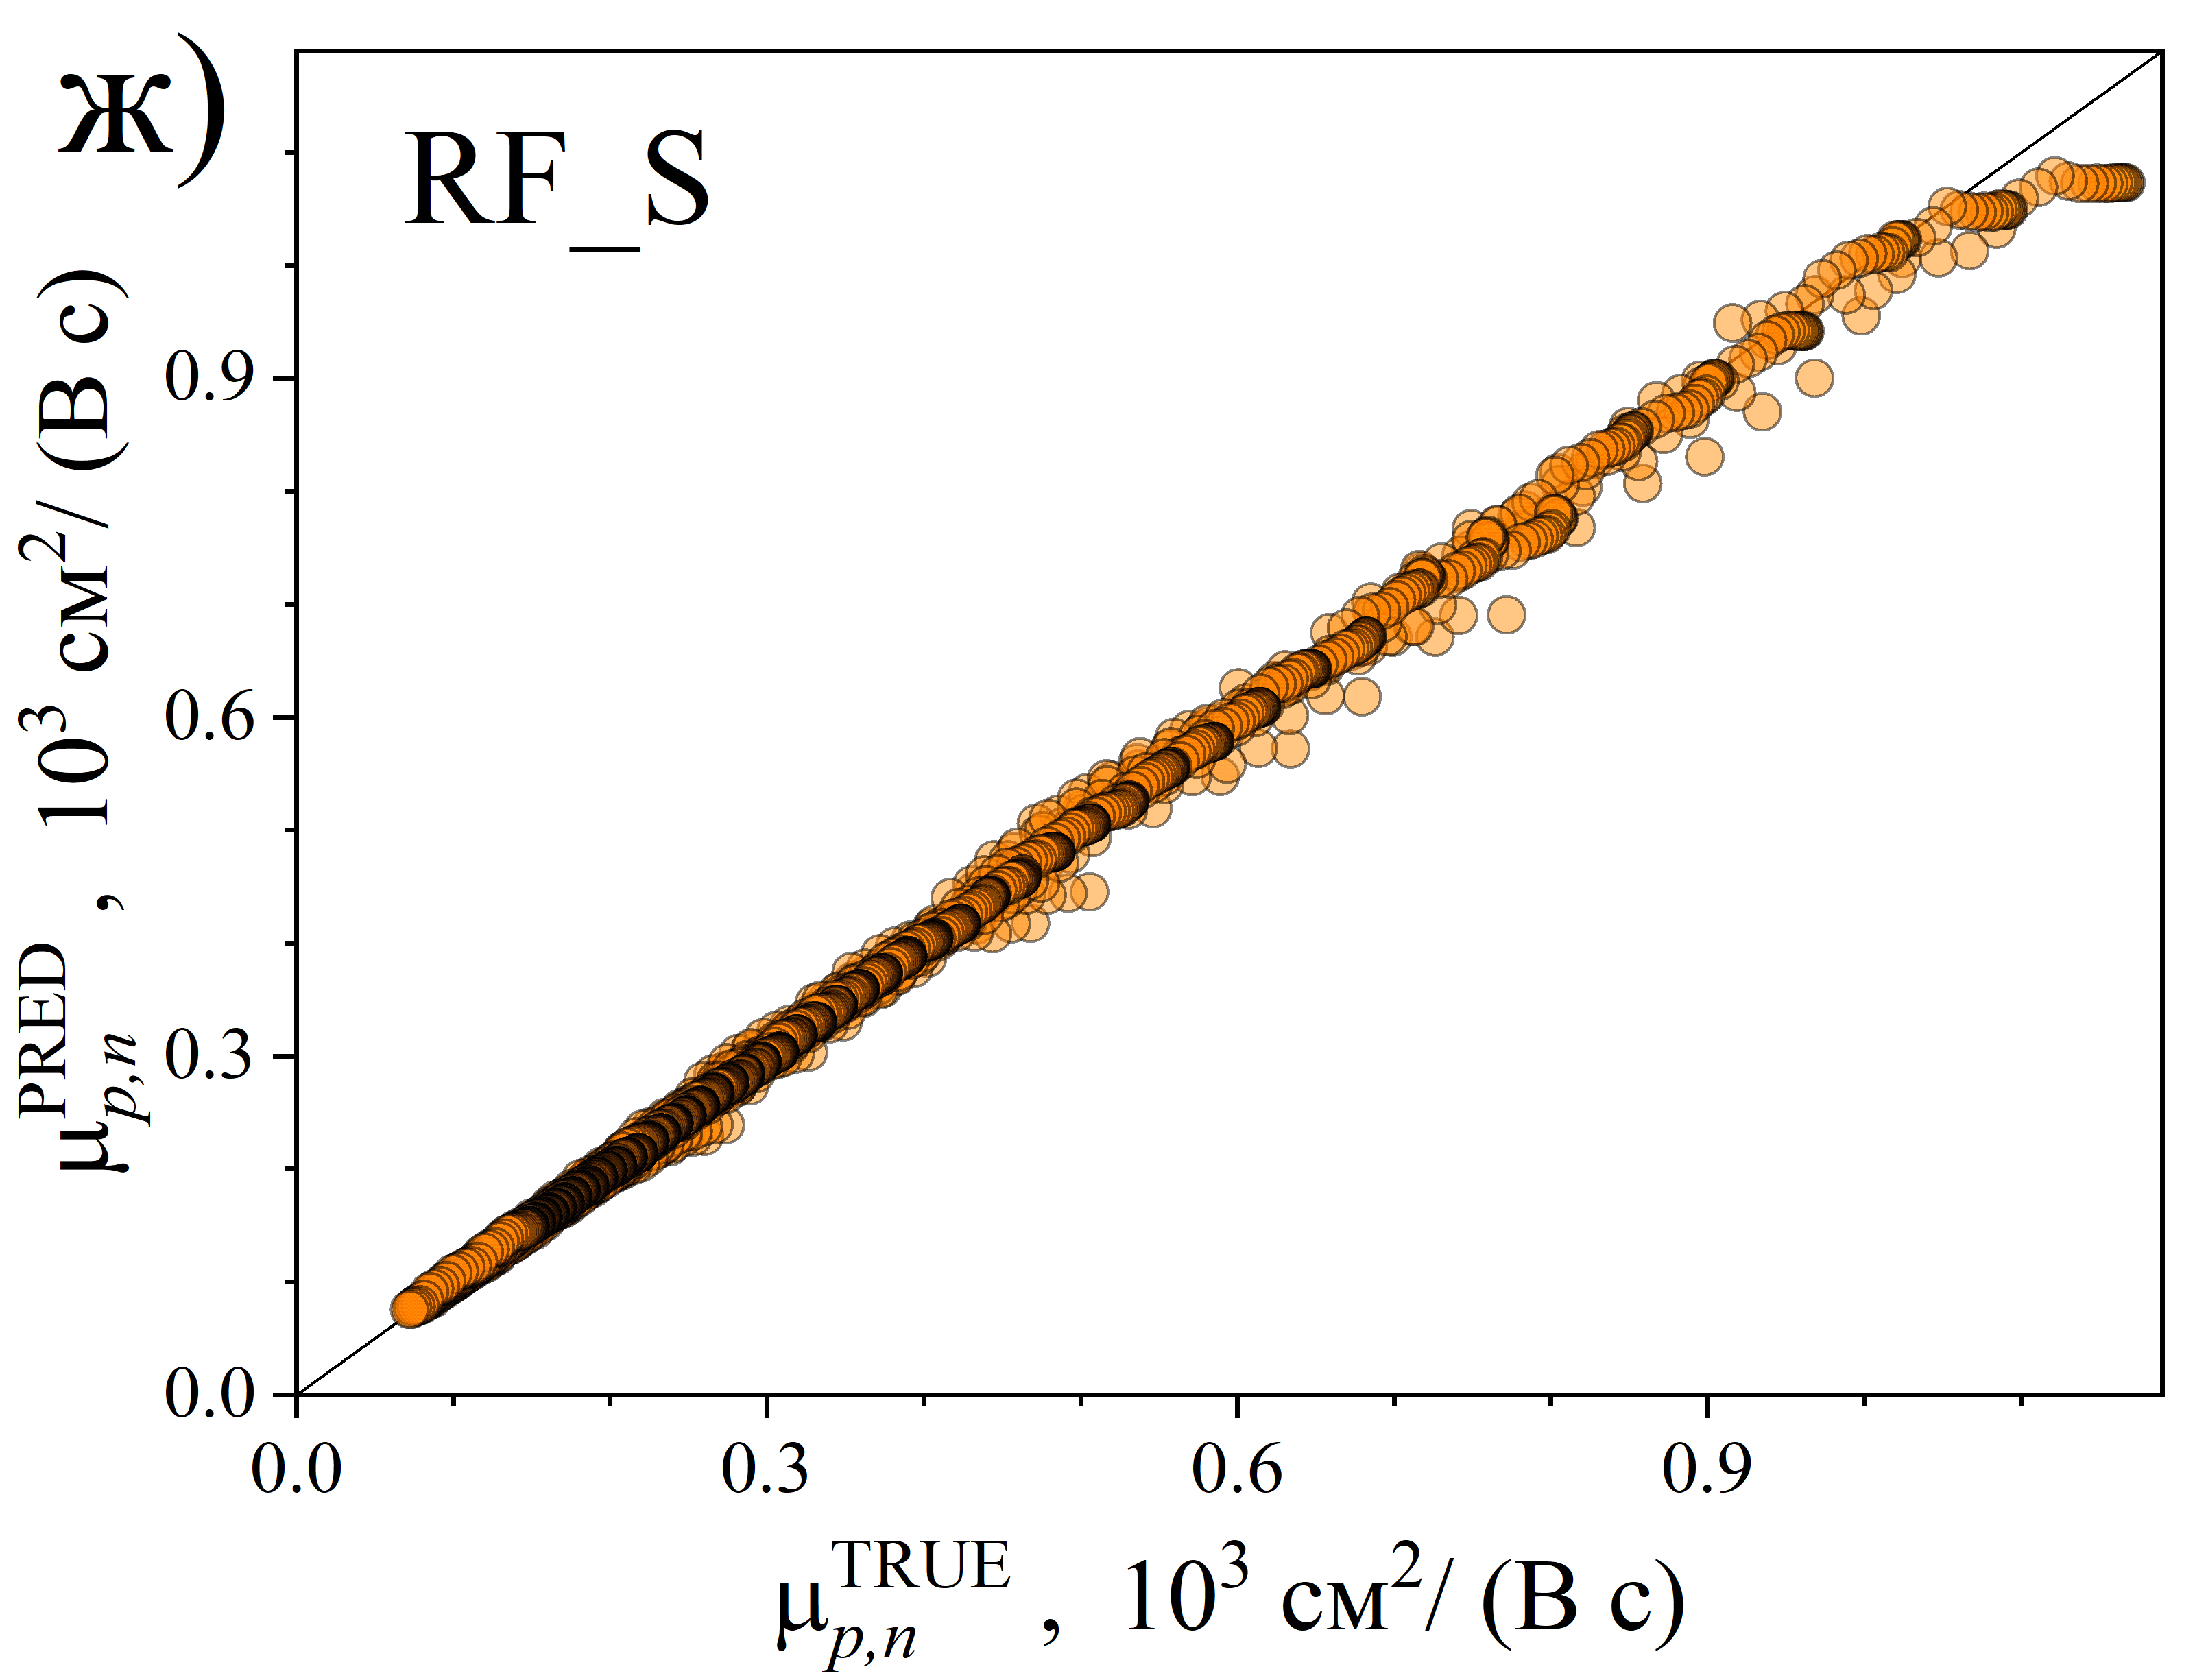
\includegraphics[width=0.35\linewidth]{RFSpn.png}
	  \caption{Діаграми розсіювання, що порівнюють еталонні значення рухливості із значеннями, передбаченими RF моделями
       на тестовому наборі даних.
       Представлені випадки оцінки рухливості електронів (а--г) та дірок (д--ж), коли вони є
       основними (а, б, д, е) та неосновними (в, г, є, ж) носіями заряду.
       Попередня підготовка даних передбачала нормування (а, в, д, є) або нормалізацію (б, г, е, ж).
}\label{figRF}
\end{figure}

\begin{figure}
	\centering
     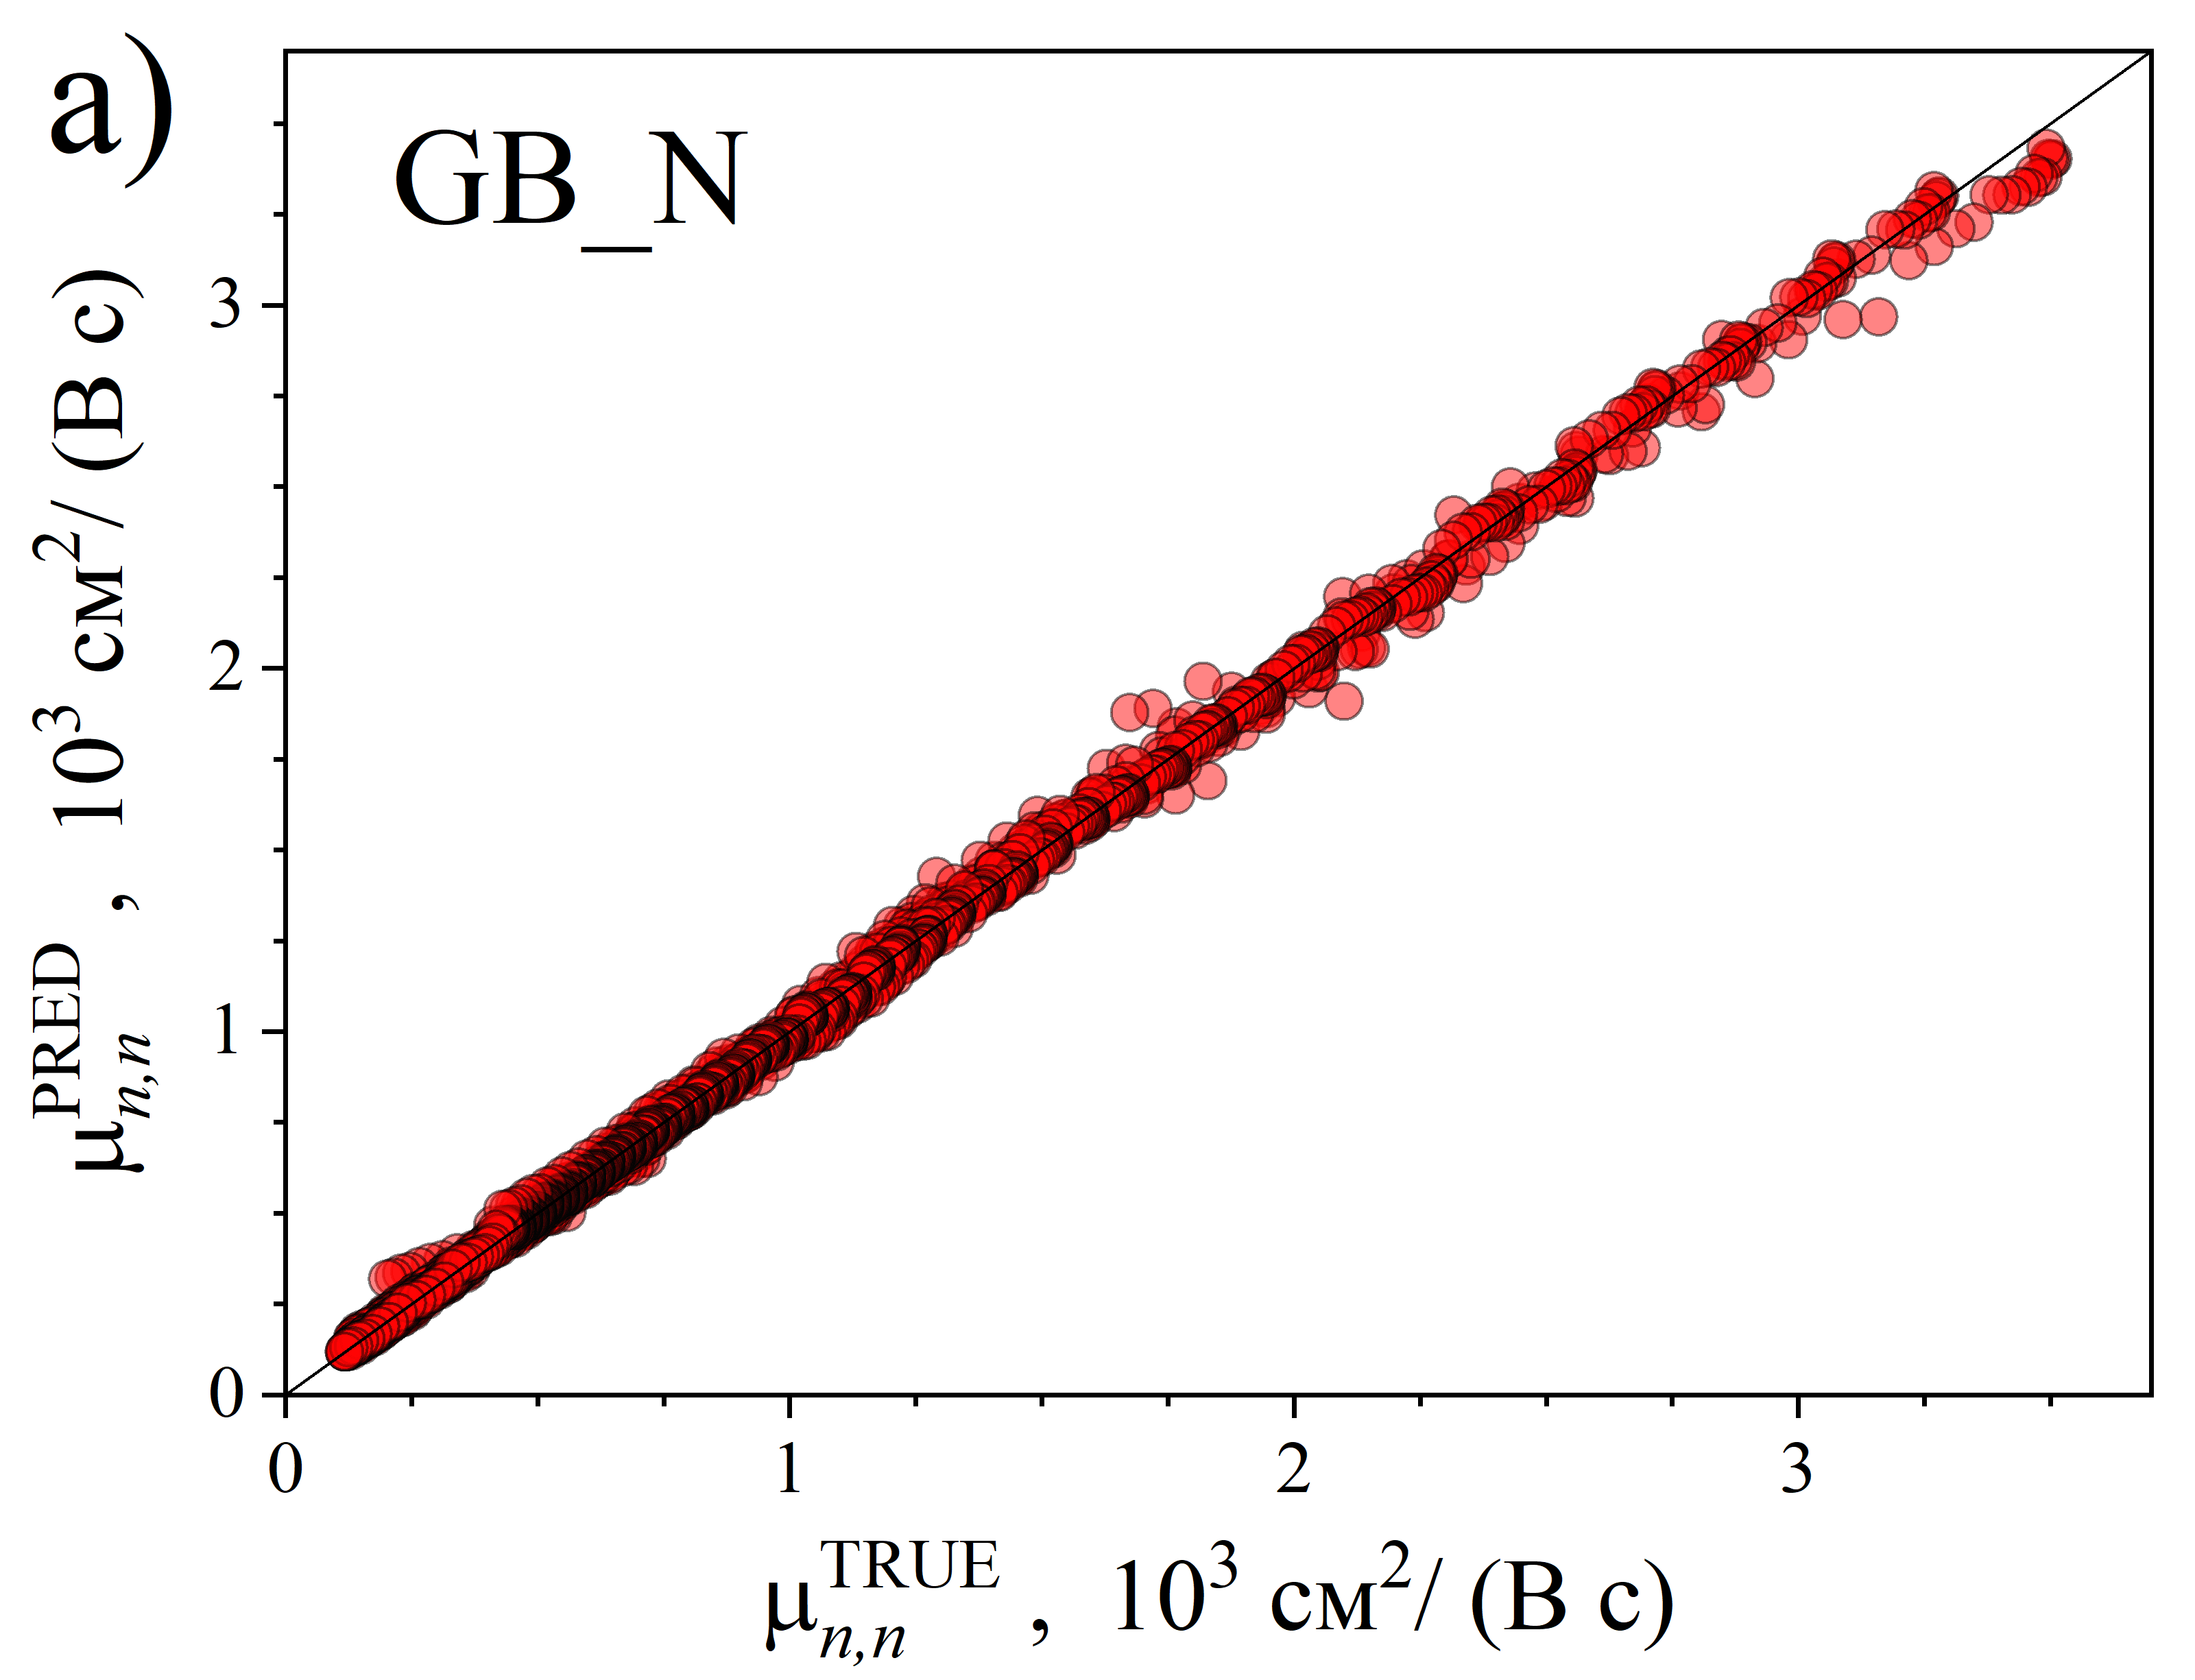
\includegraphics[width=0.35\linewidth]{GBNnn.png}\kern 20pt
     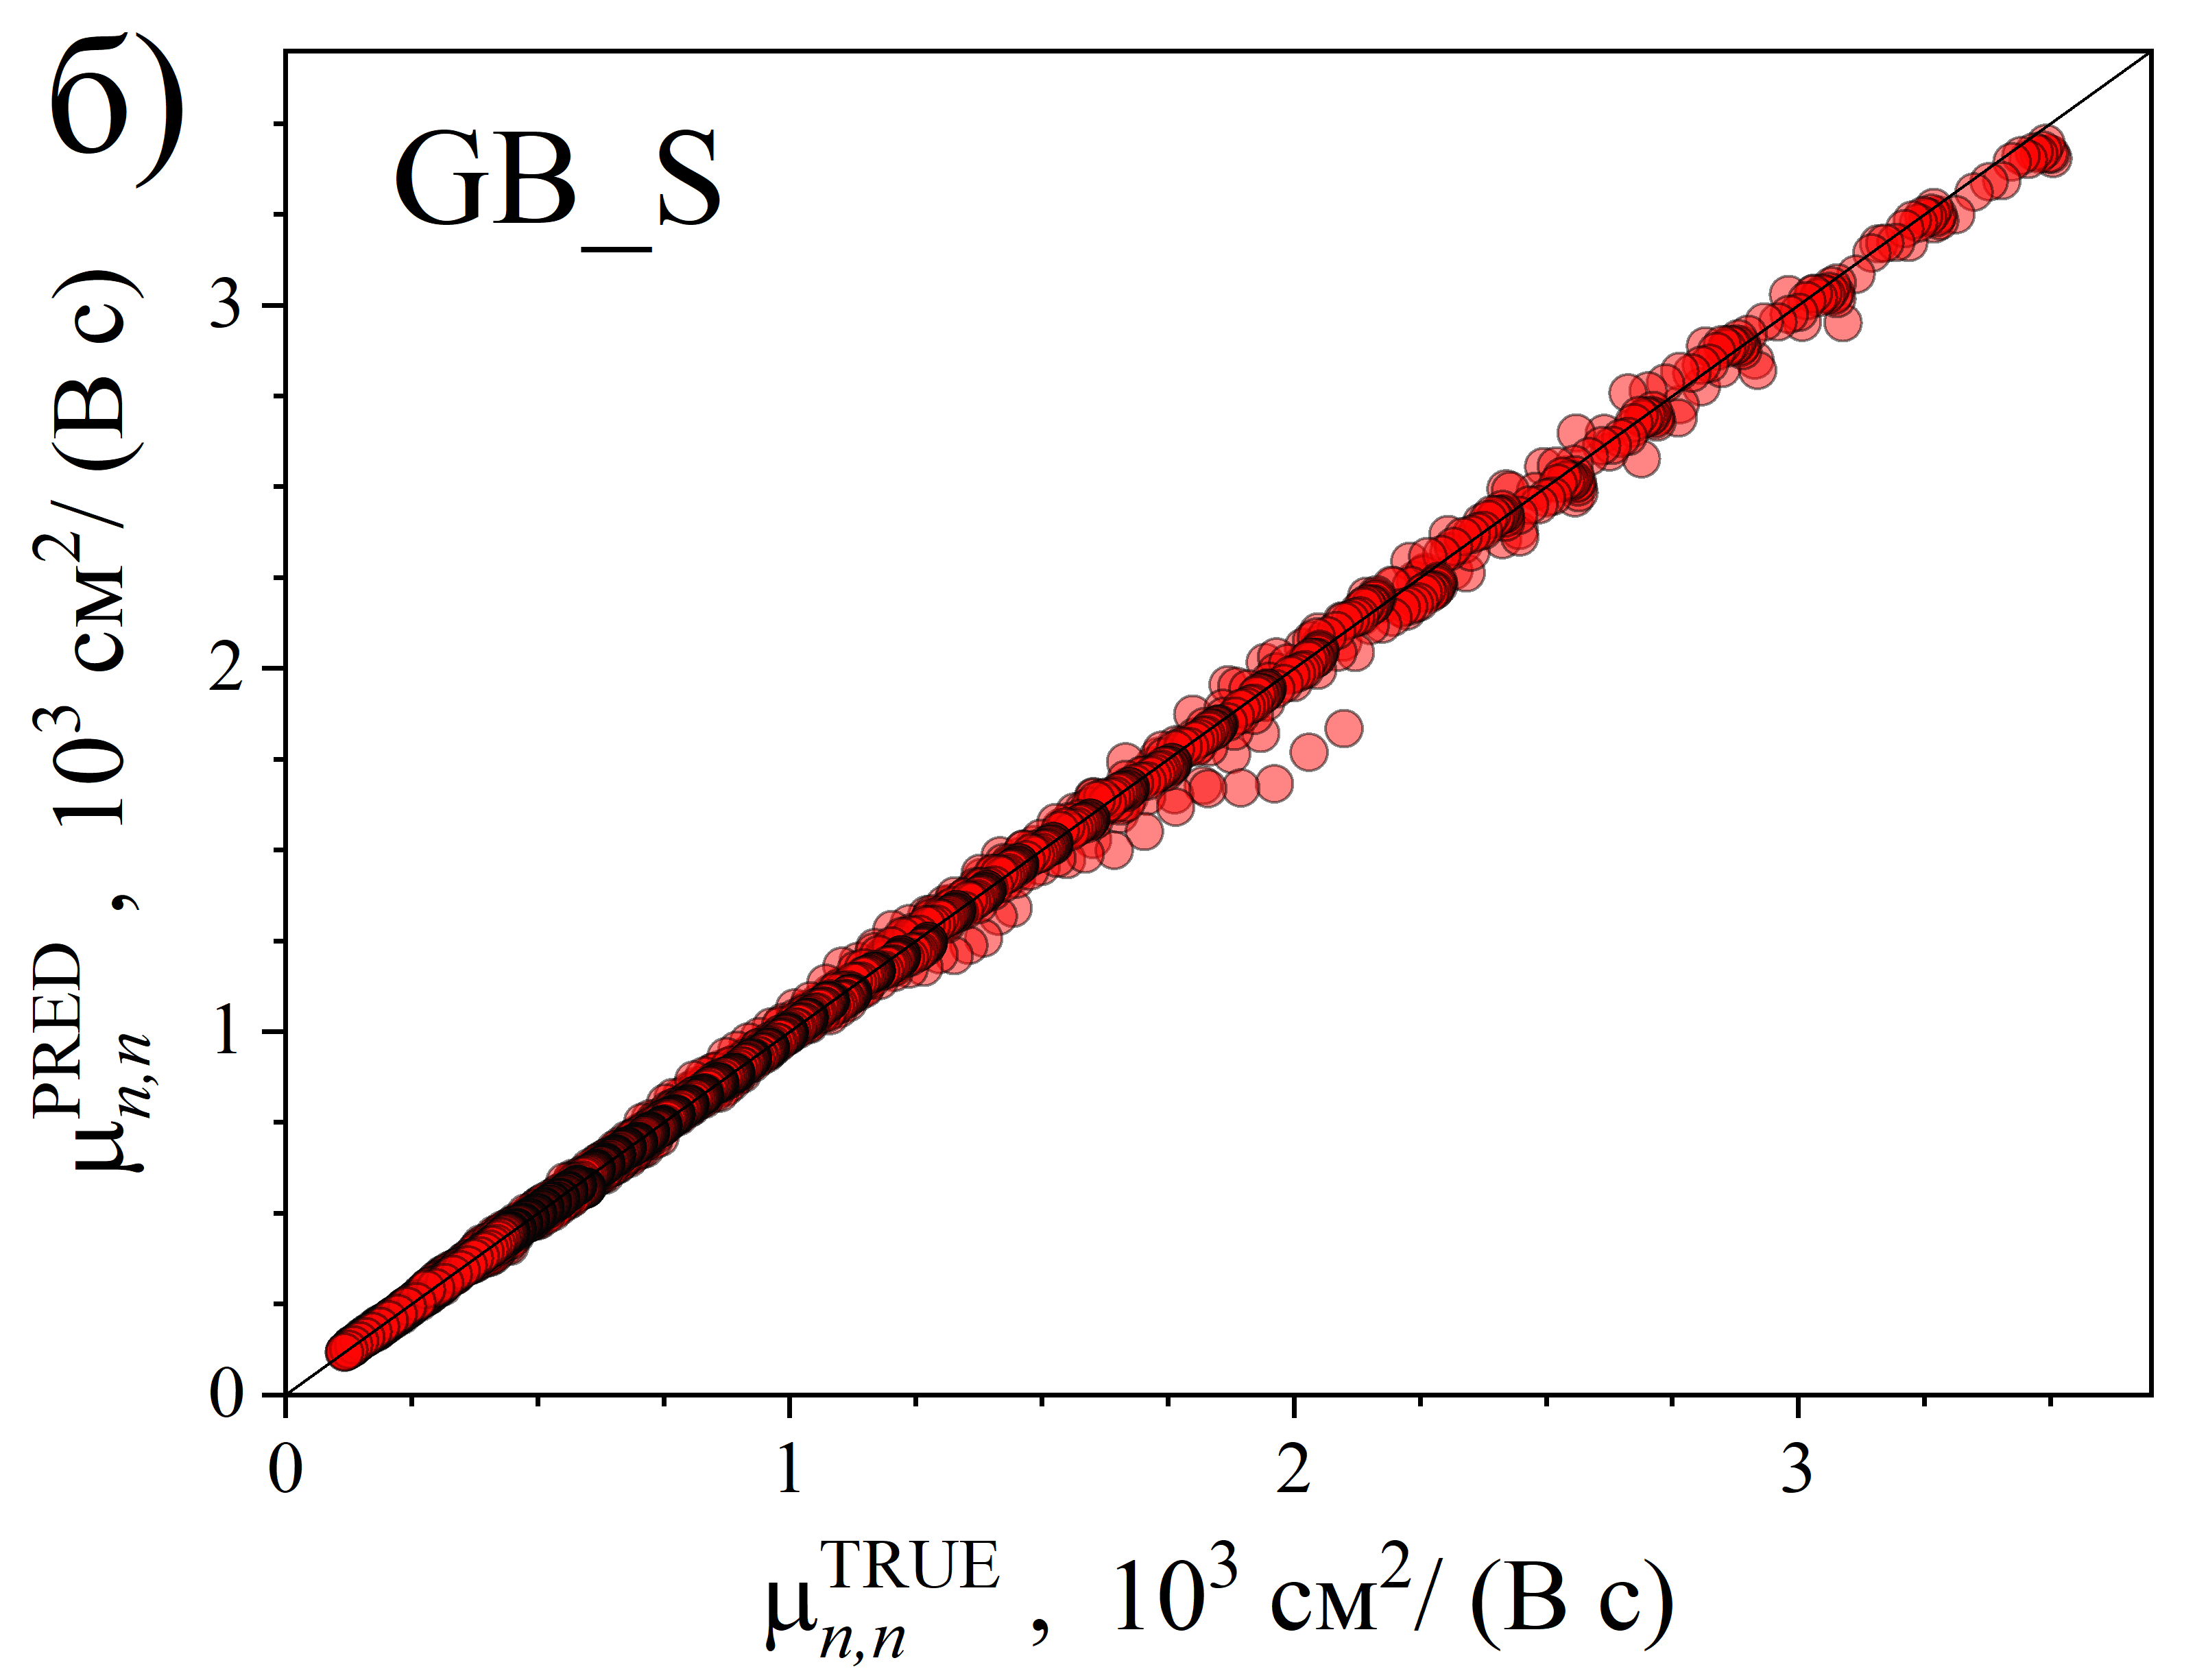
\includegraphics[width=0.35\linewidth]{GBSnn.png}
     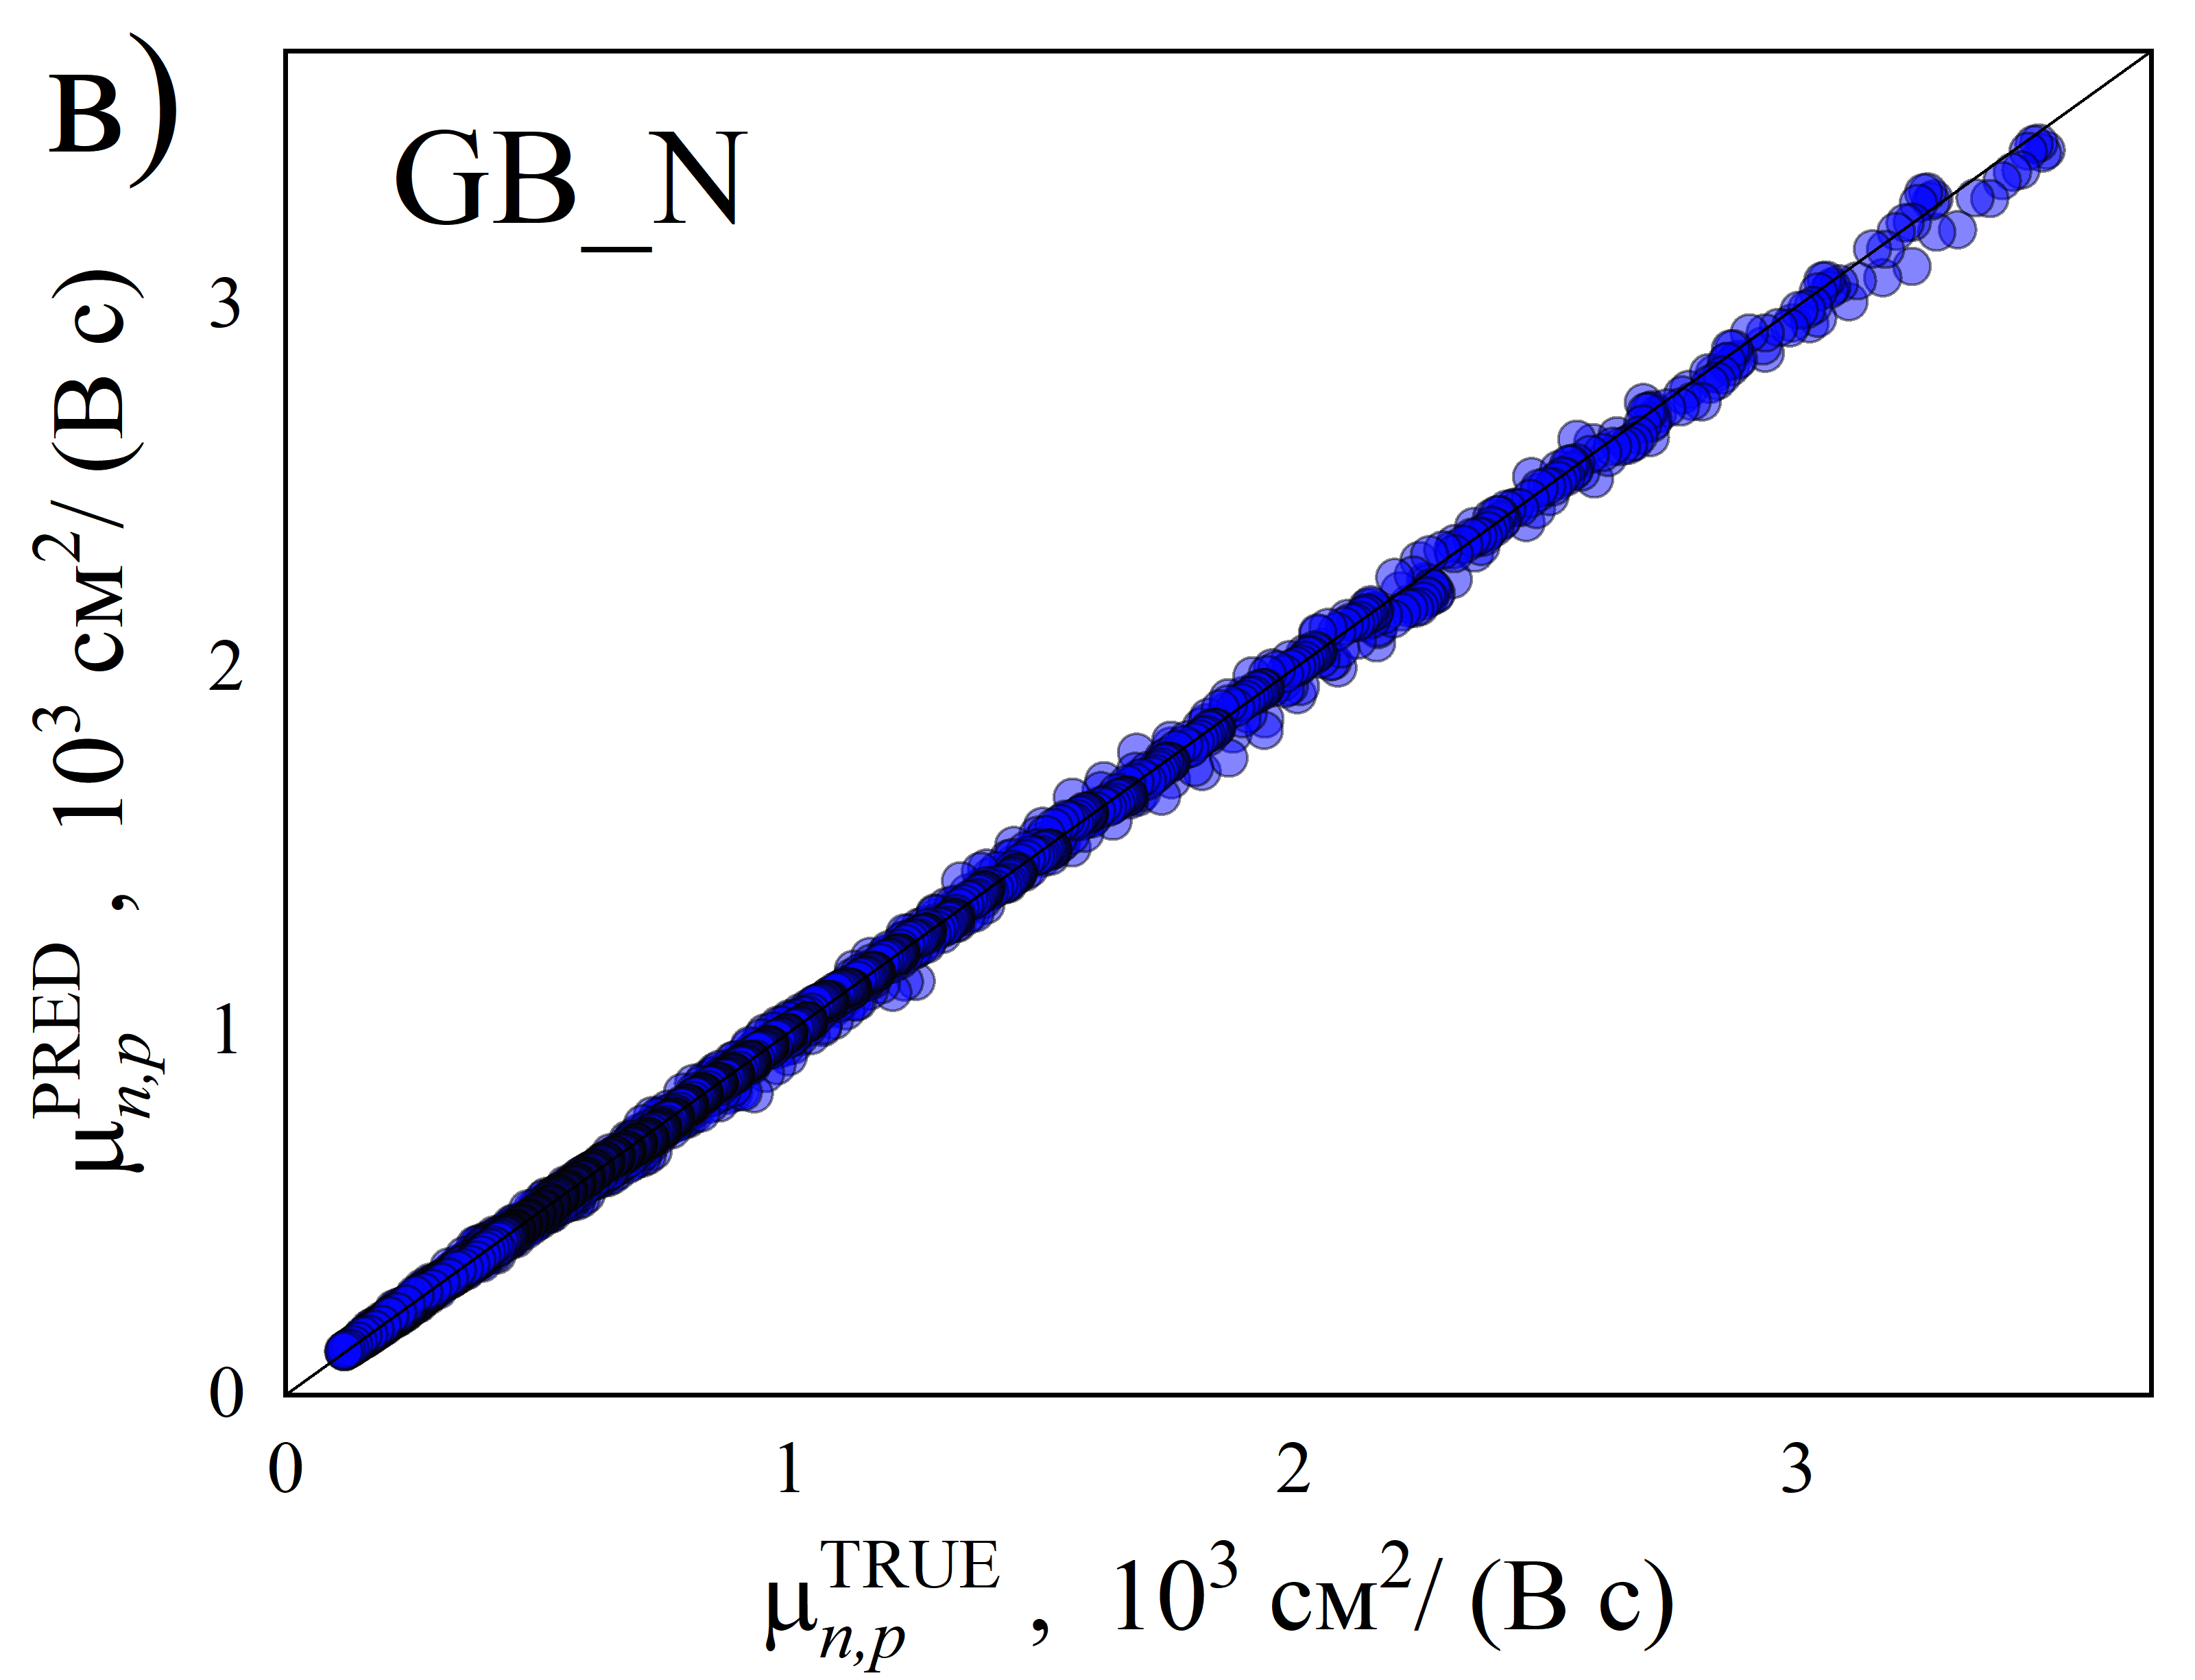
\includegraphics[width=0.35\linewidth]{GBNnp.png}\kern 20pt
     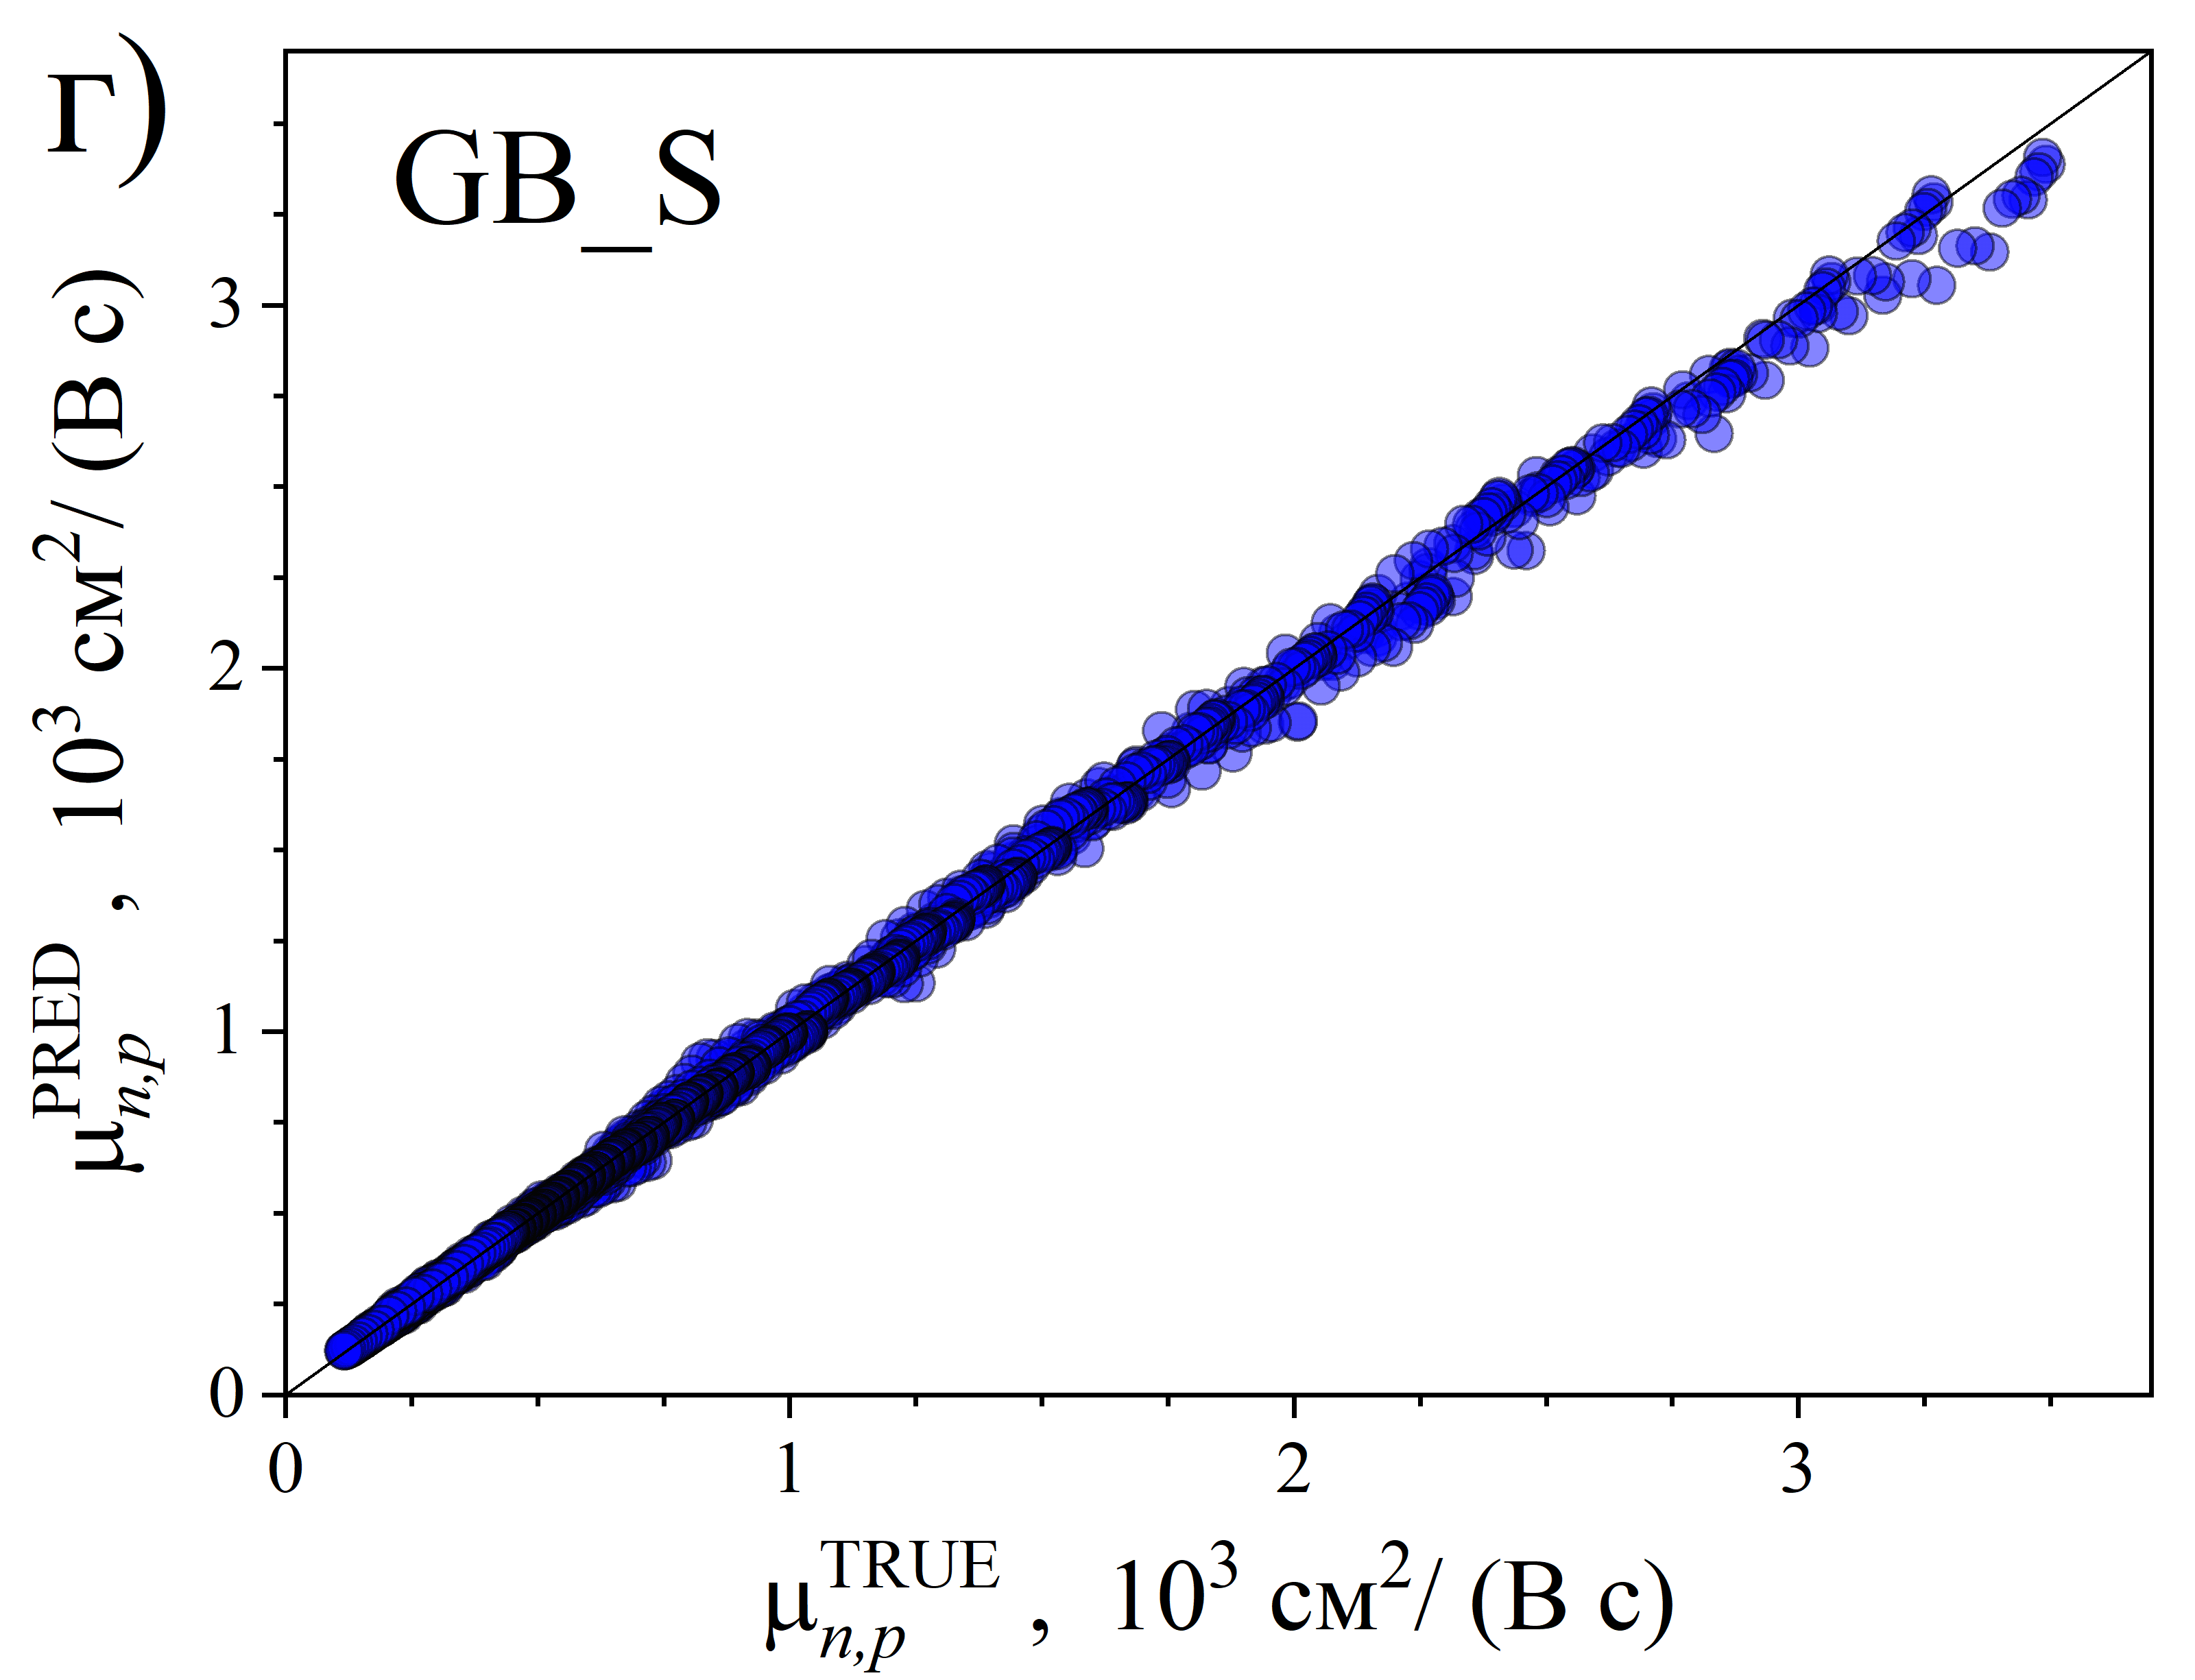
\includegraphics[width=0.35\linewidth]{GBSnp.png}
     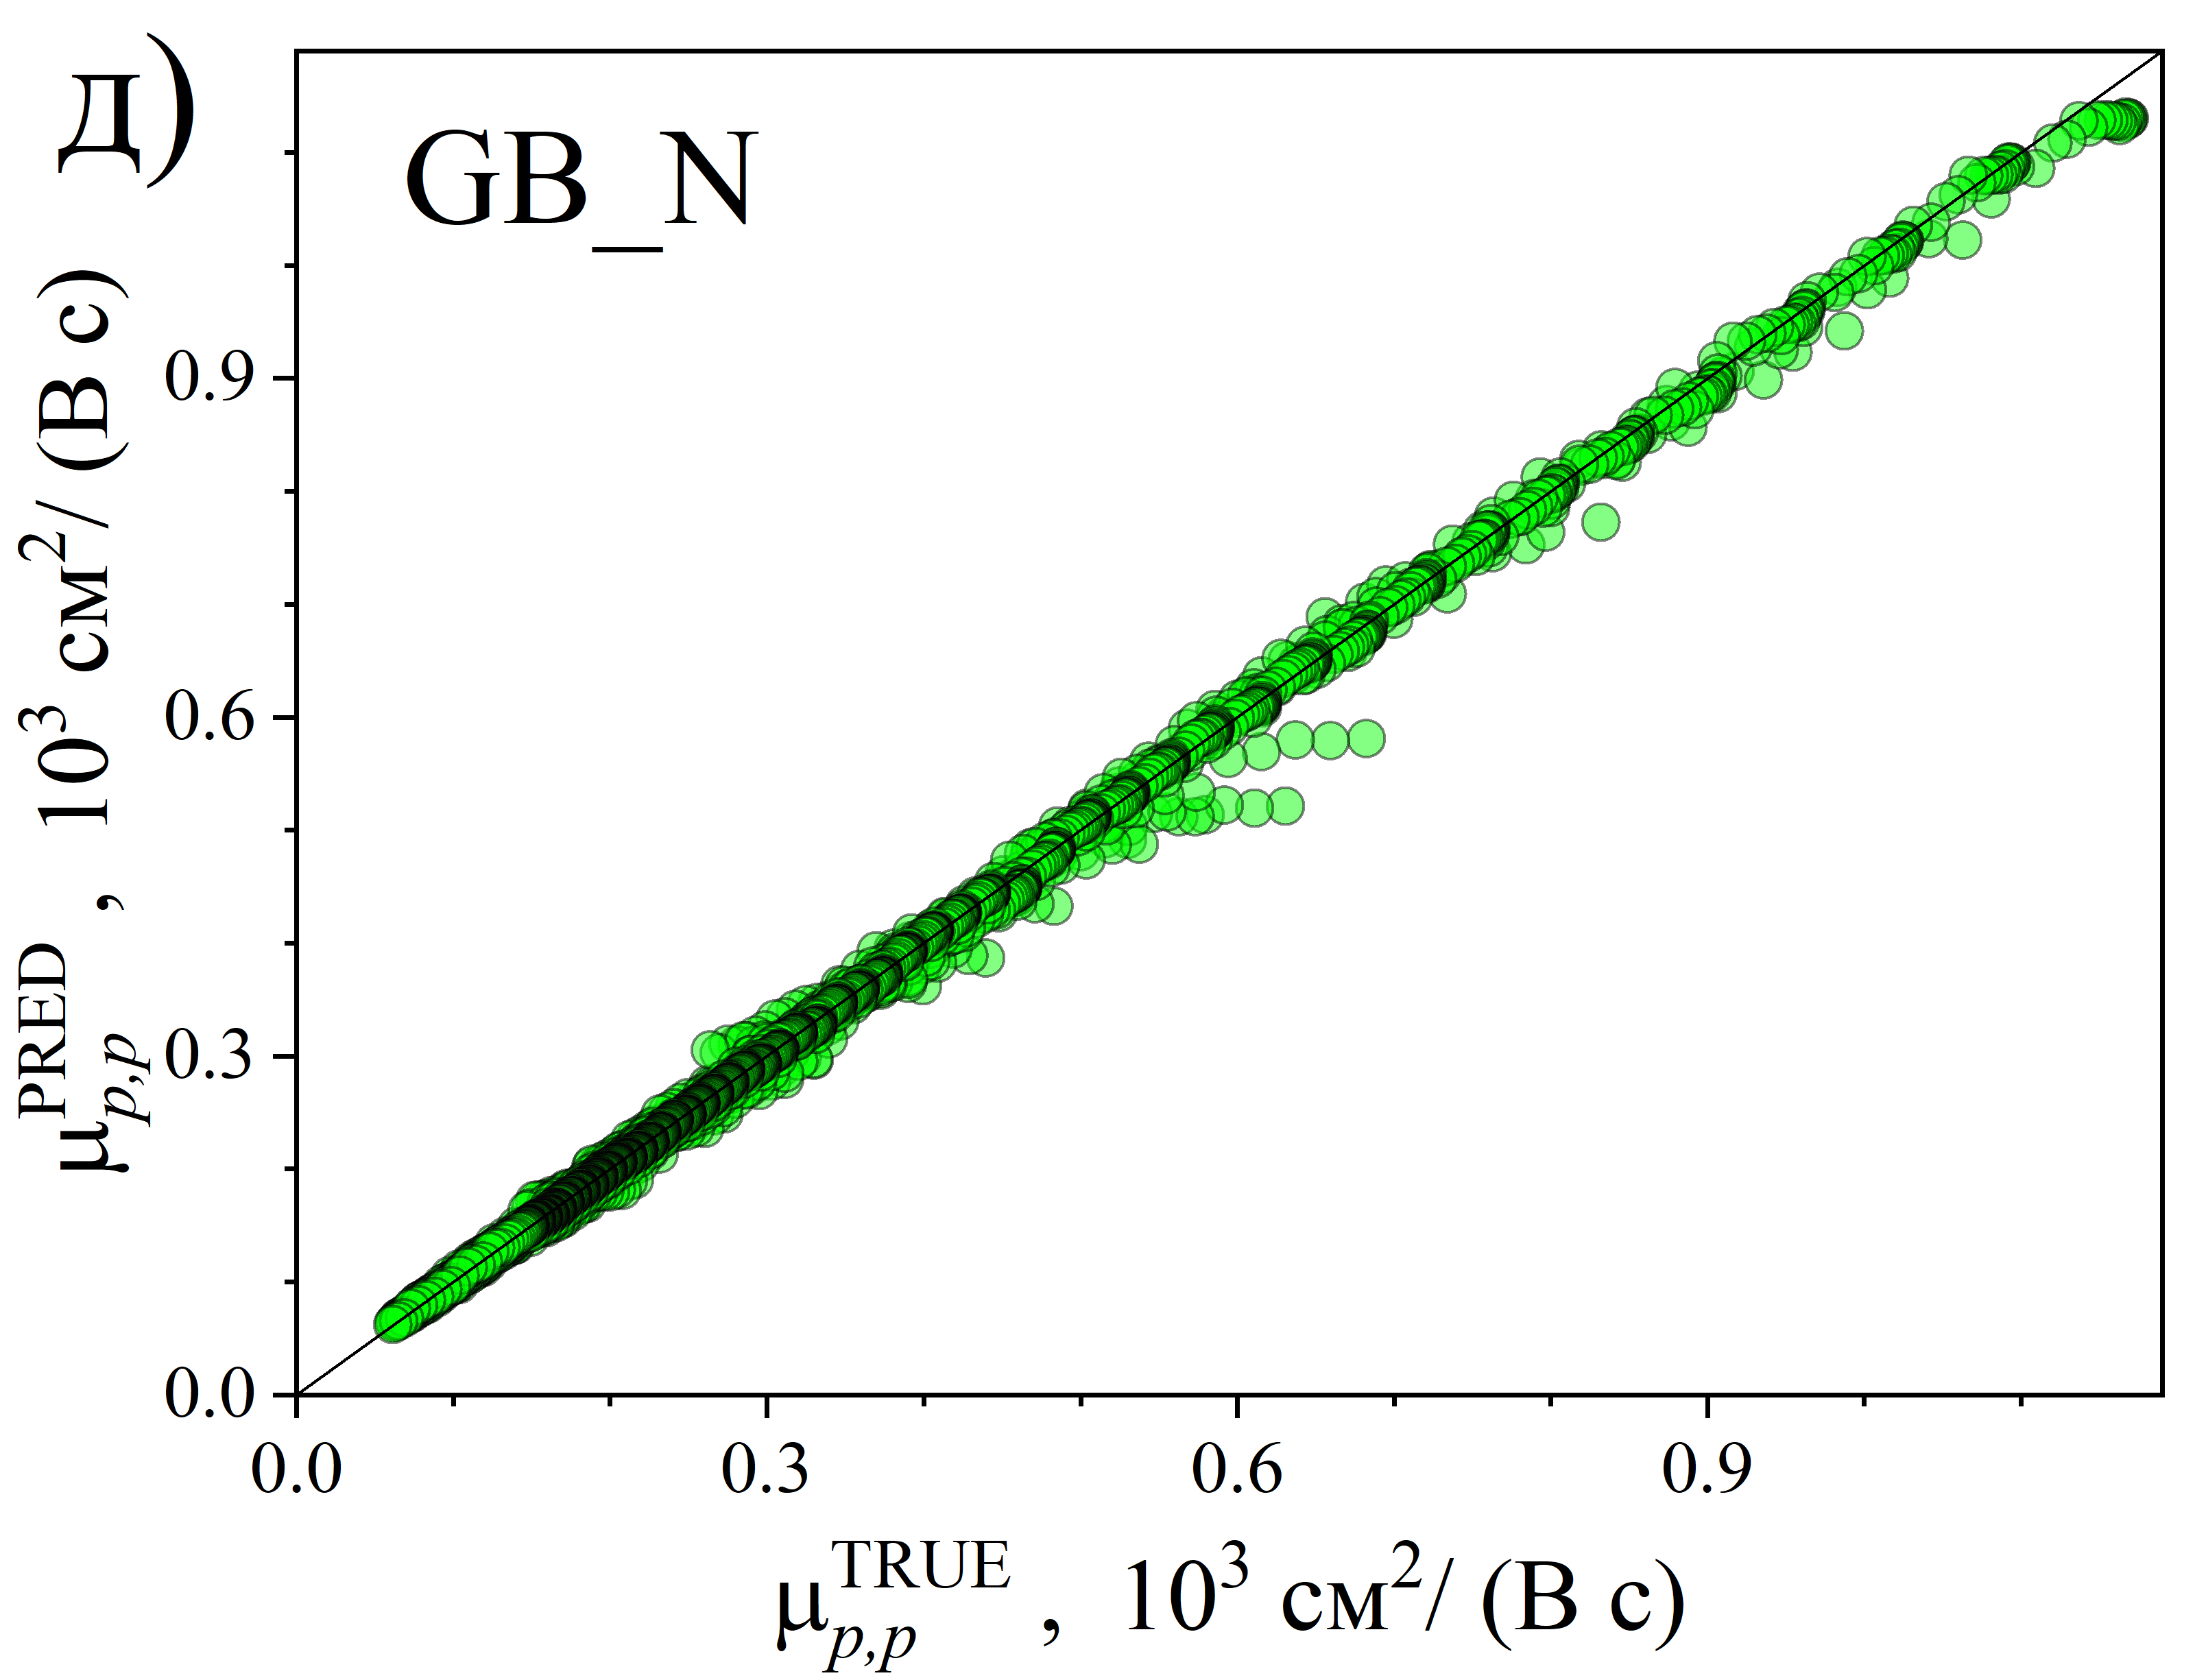
\includegraphics[width=0.35\linewidth]{GBNpp.png}\kern 20pt
     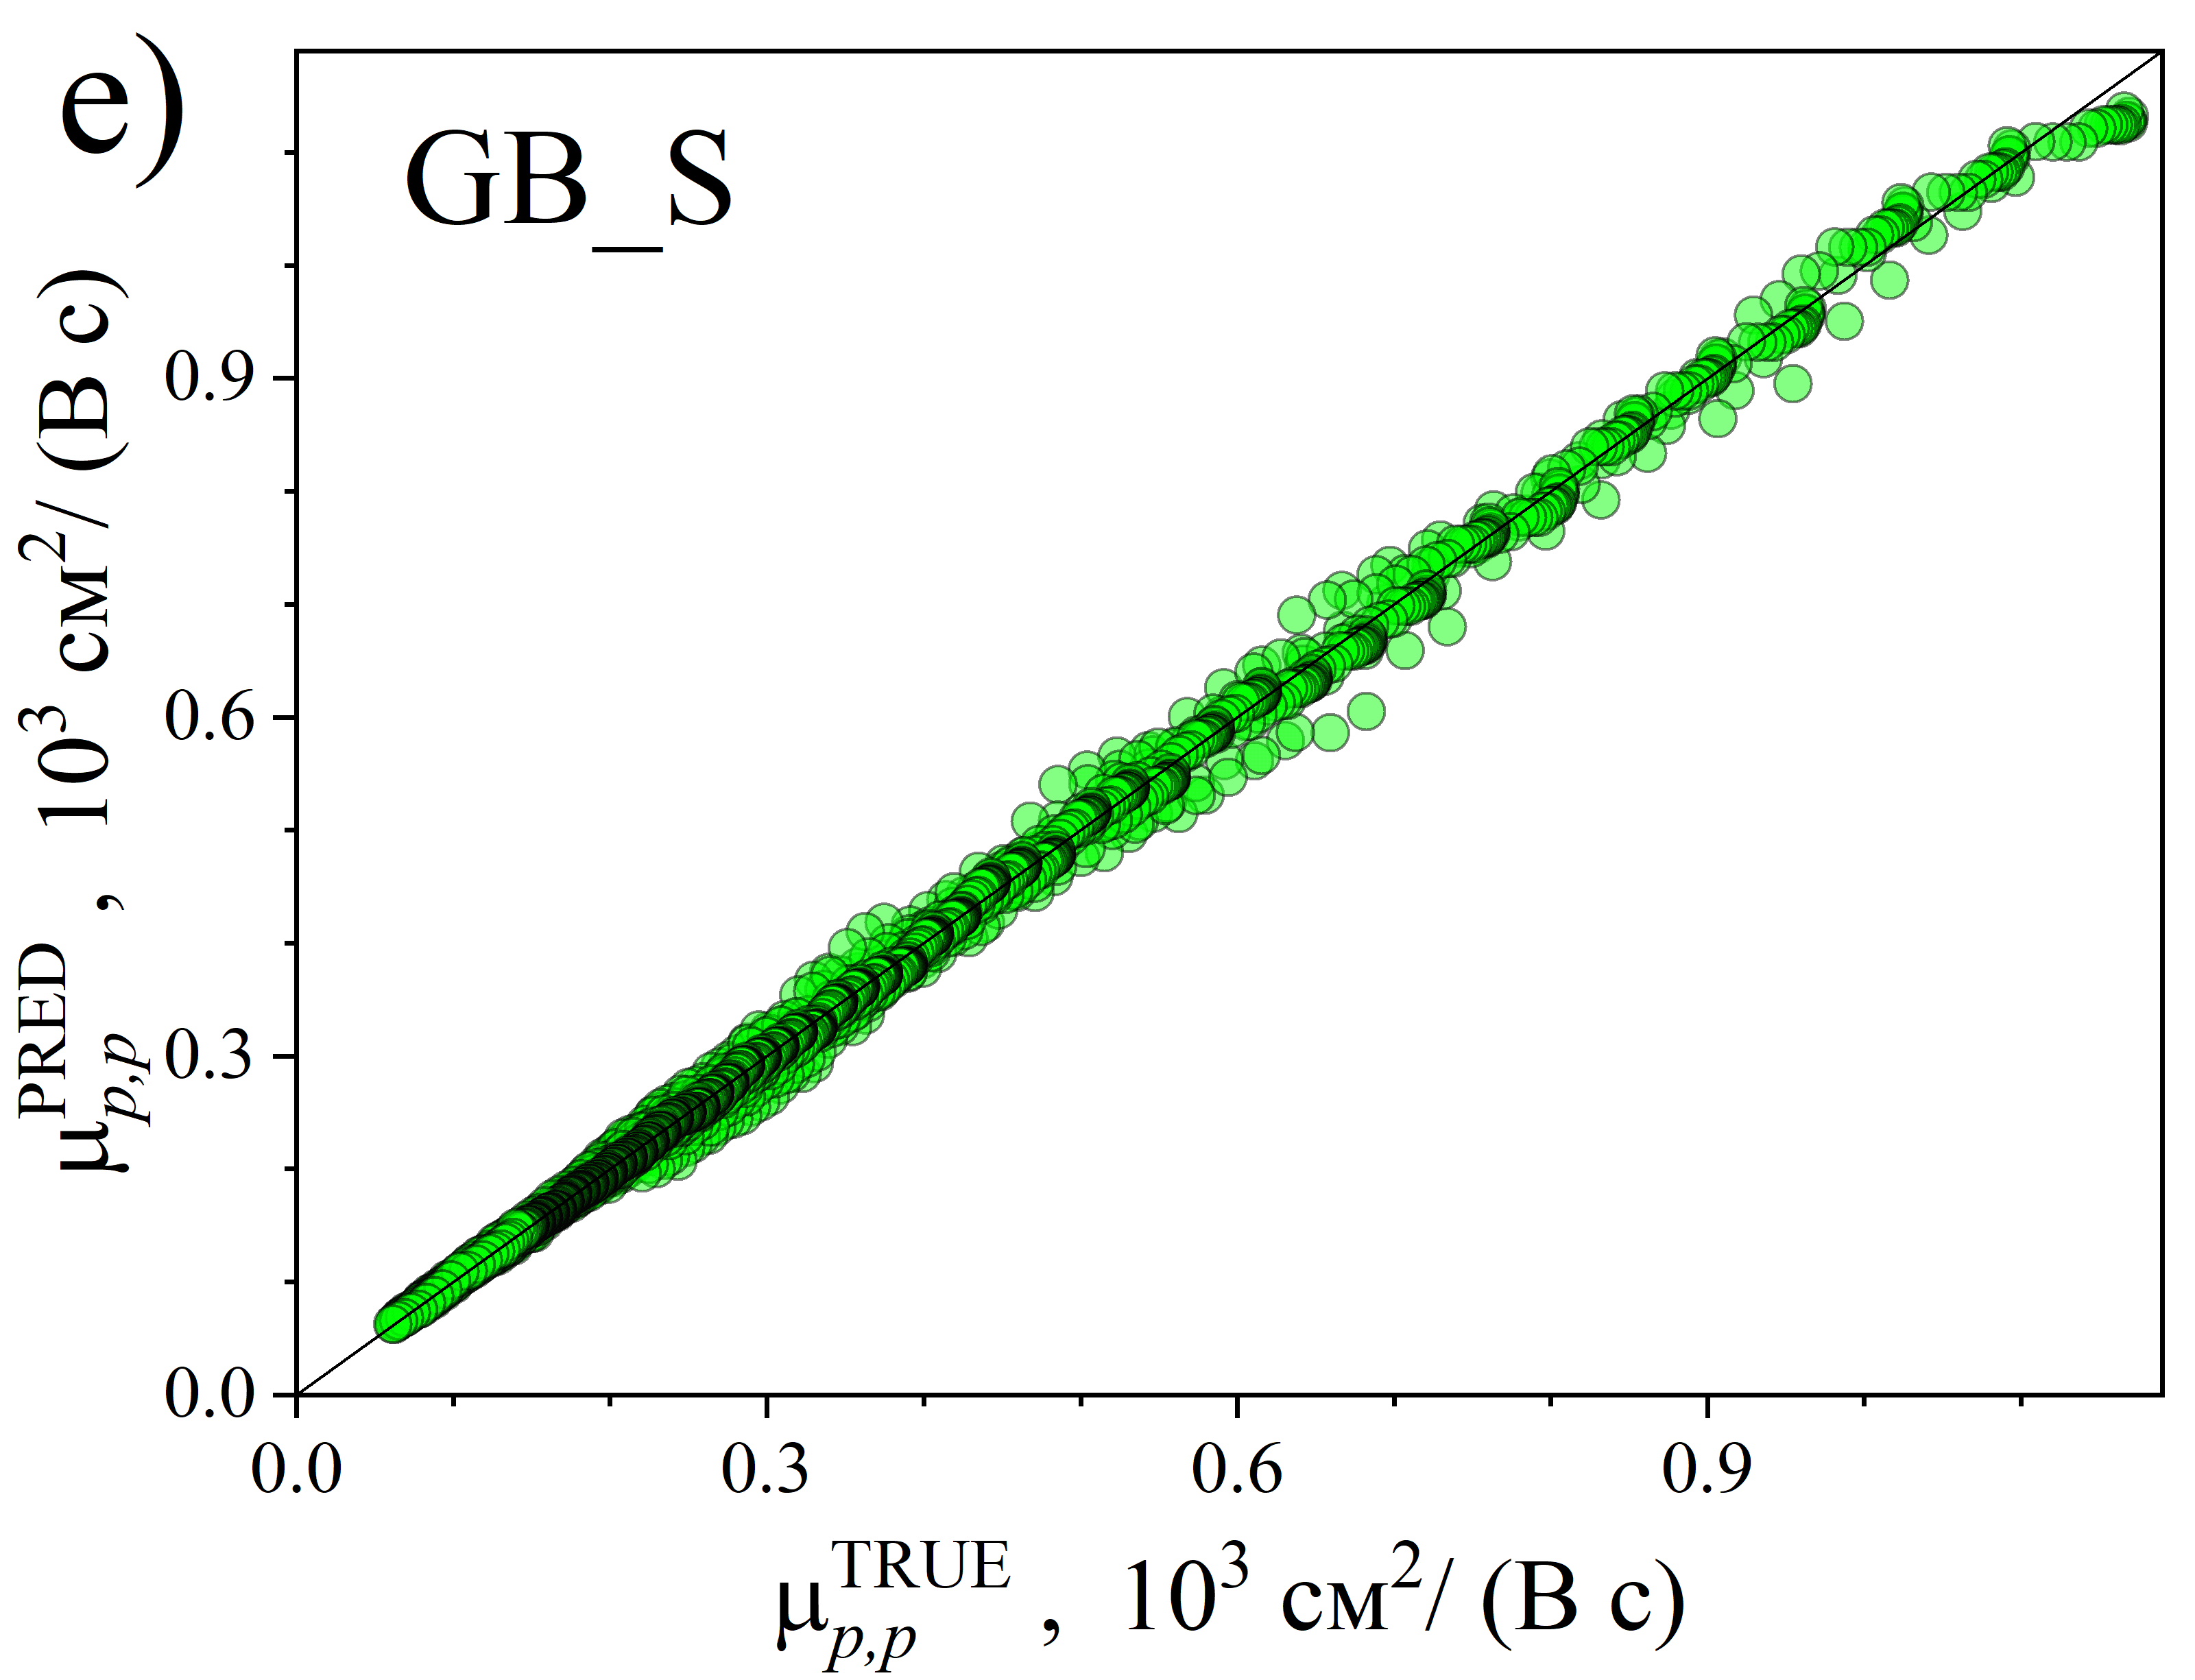
\includegraphics[width=0.35\linewidth]{GBSpp.png}
     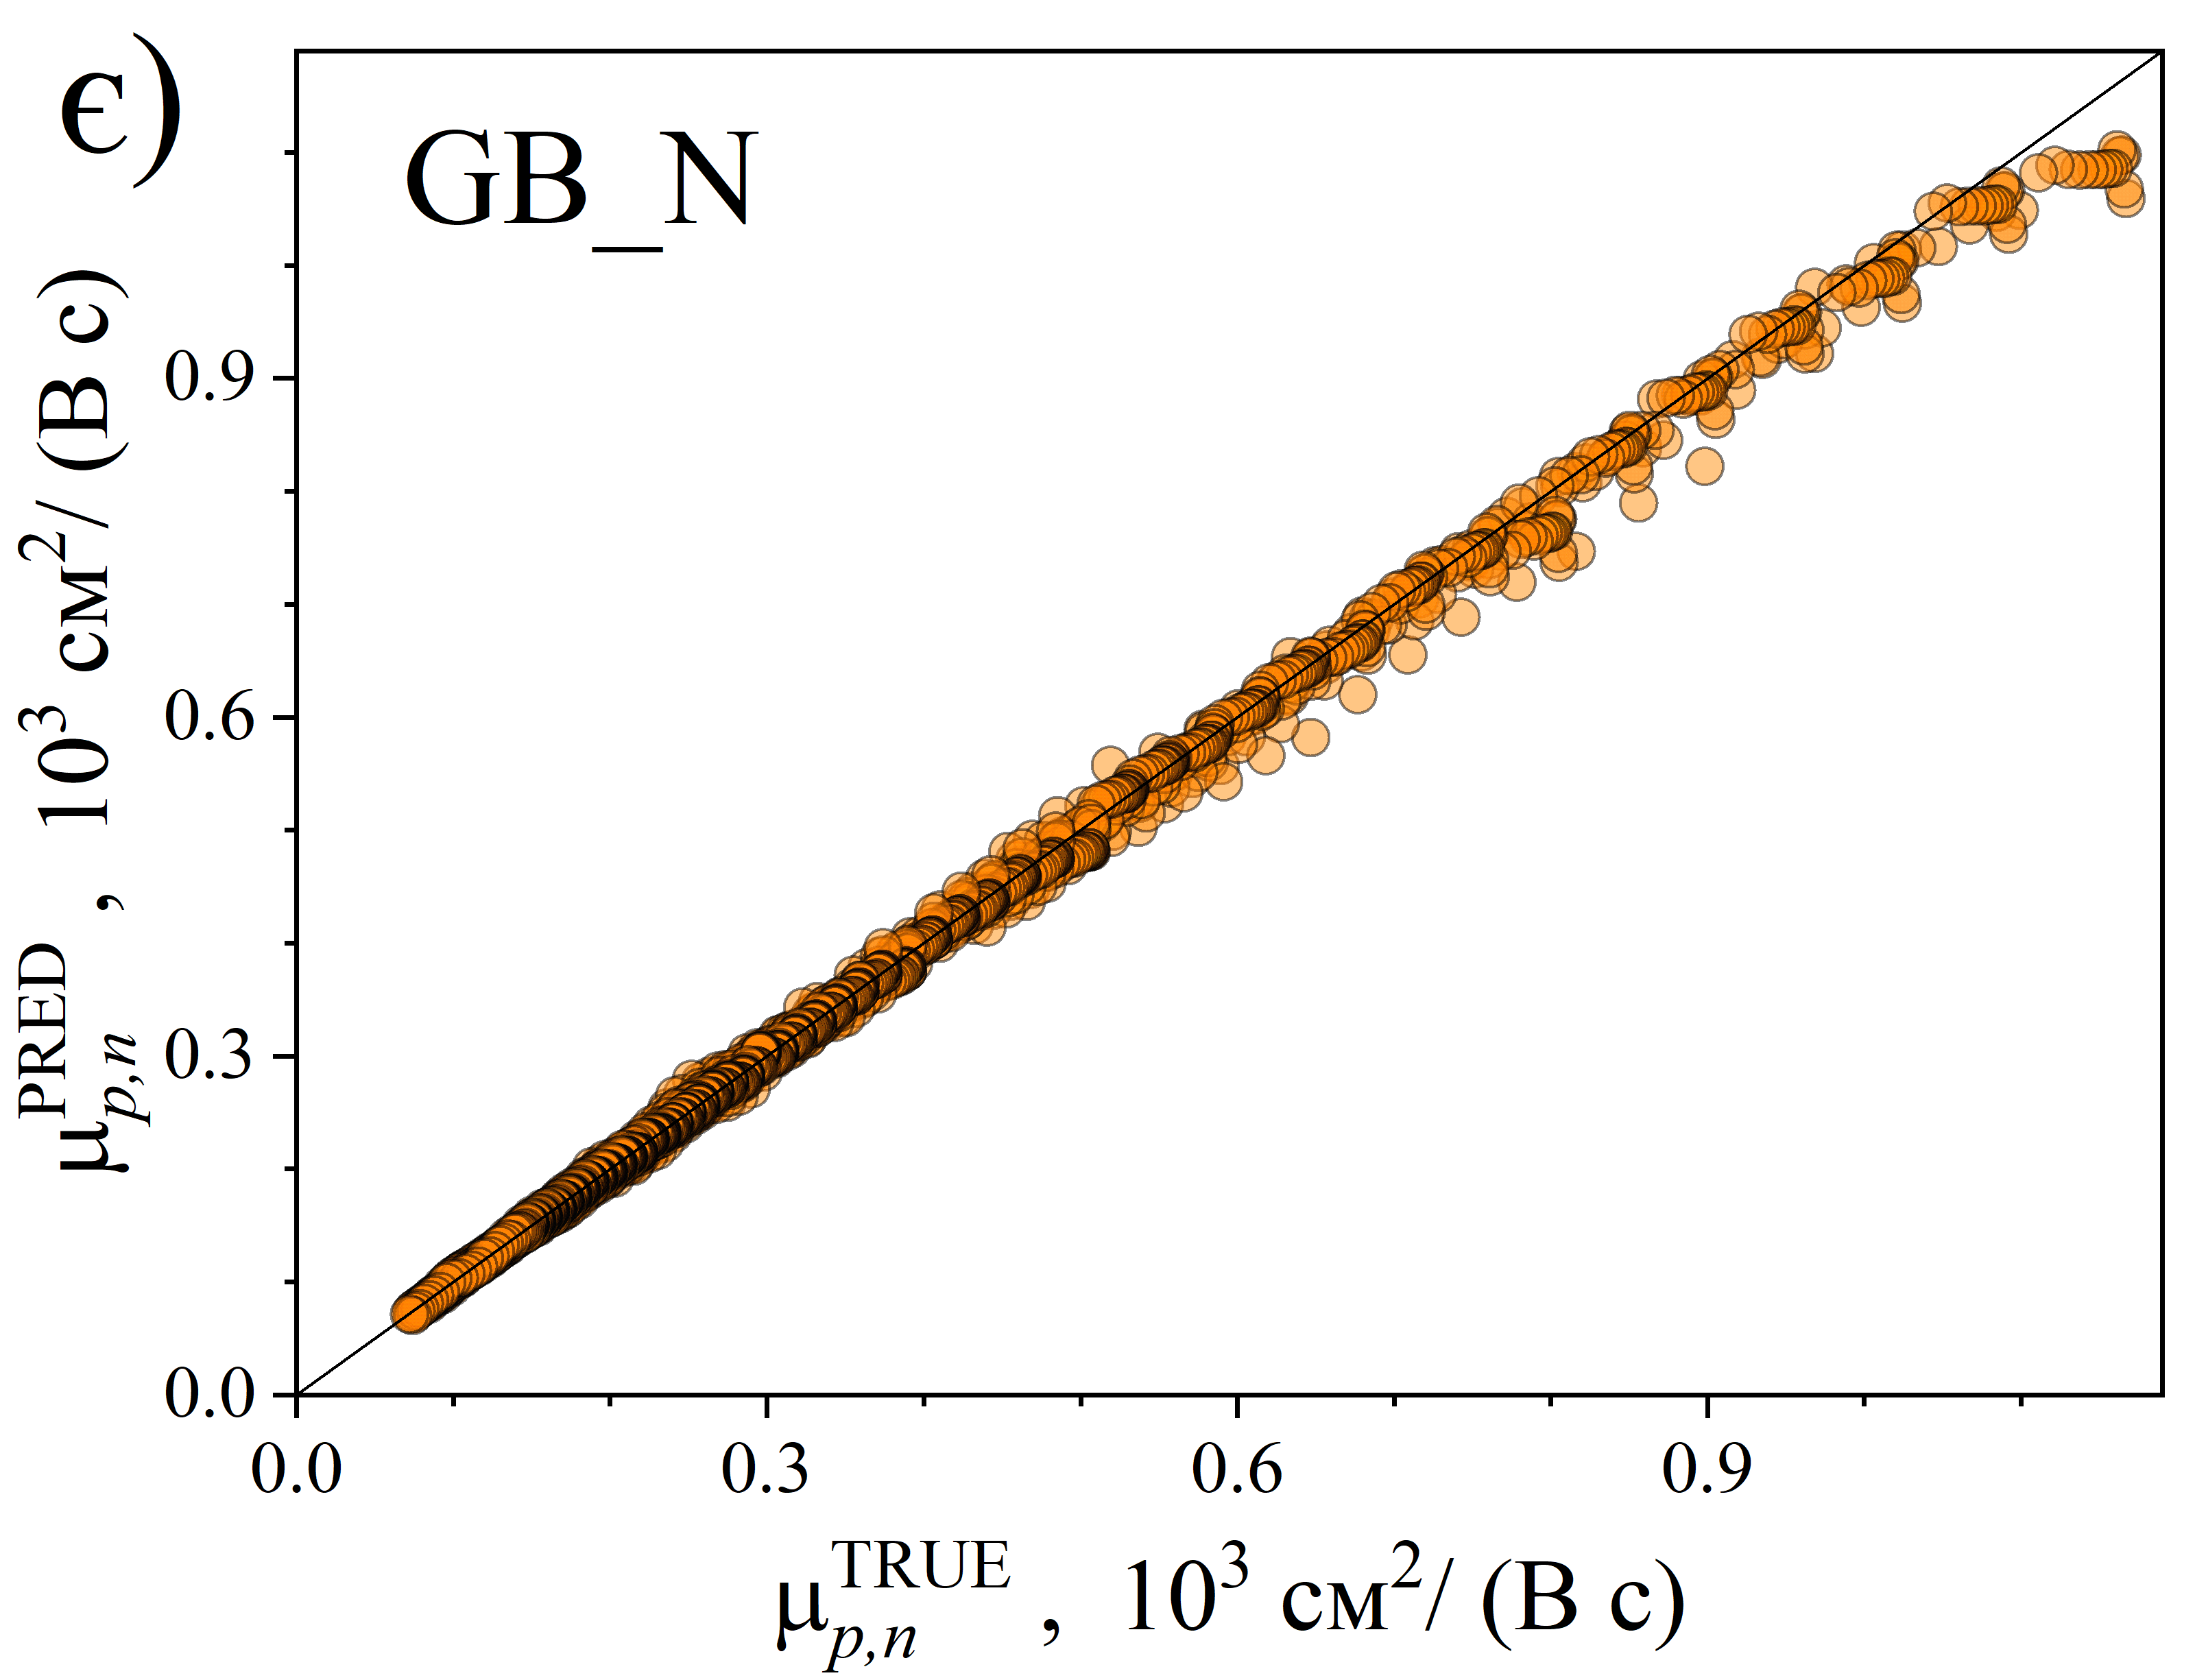
\includegraphics[width=0.35\linewidth]{GBNpn.png}\kern 20pt
     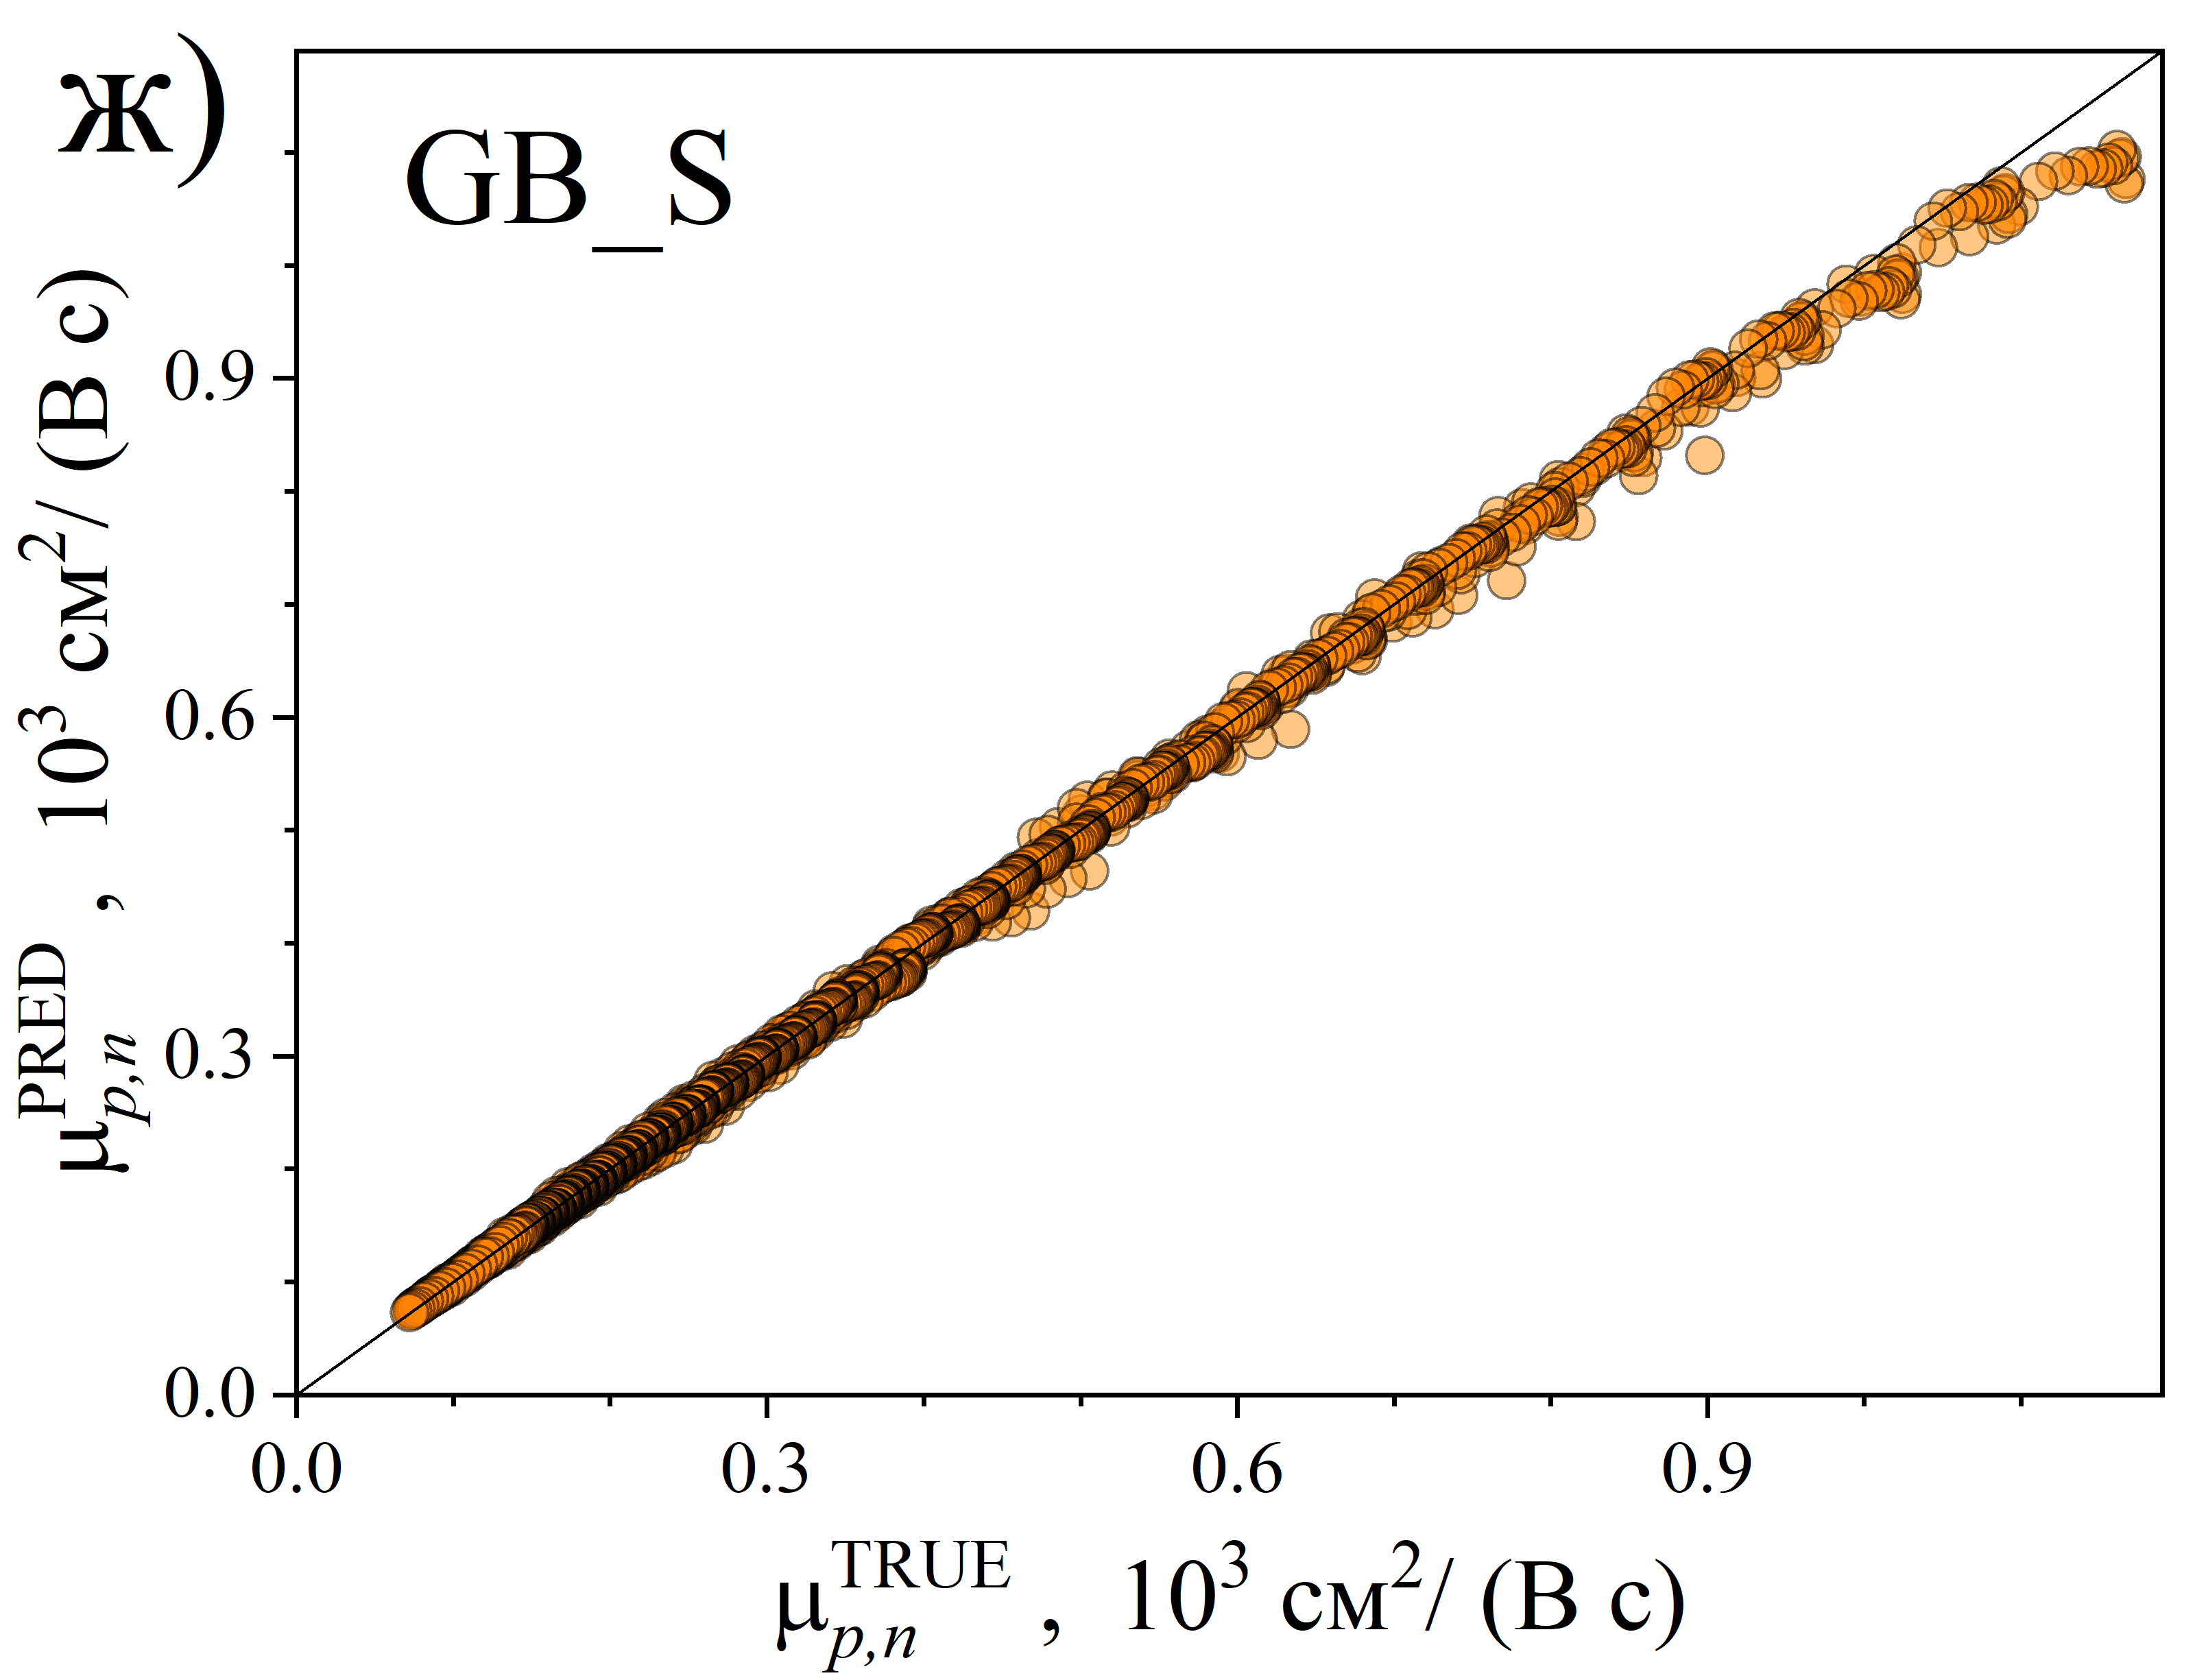
\includegraphics[width=0.35\linewidth]{GBSpn.png}
	  \caption{Діаграми розсіювання, що порівнюють еталонні значення рухливості із значеннями, передбаченими GB моделями
       на тестовому наборі даних.
       Представлені випадки оцінки рухливості електронів (а--г) та дірок (д--ж), коли вони є
       основними (а, б, д, е) та неосновними (в, г, є, ж) носіями заряду.
       Попередня підготовка даних передбачала нормування (а, в, д, є) або нормалізацію (б, г, е, ж).
}\label{figGB}
\end{figure}


\begin{figure}
	\centering
     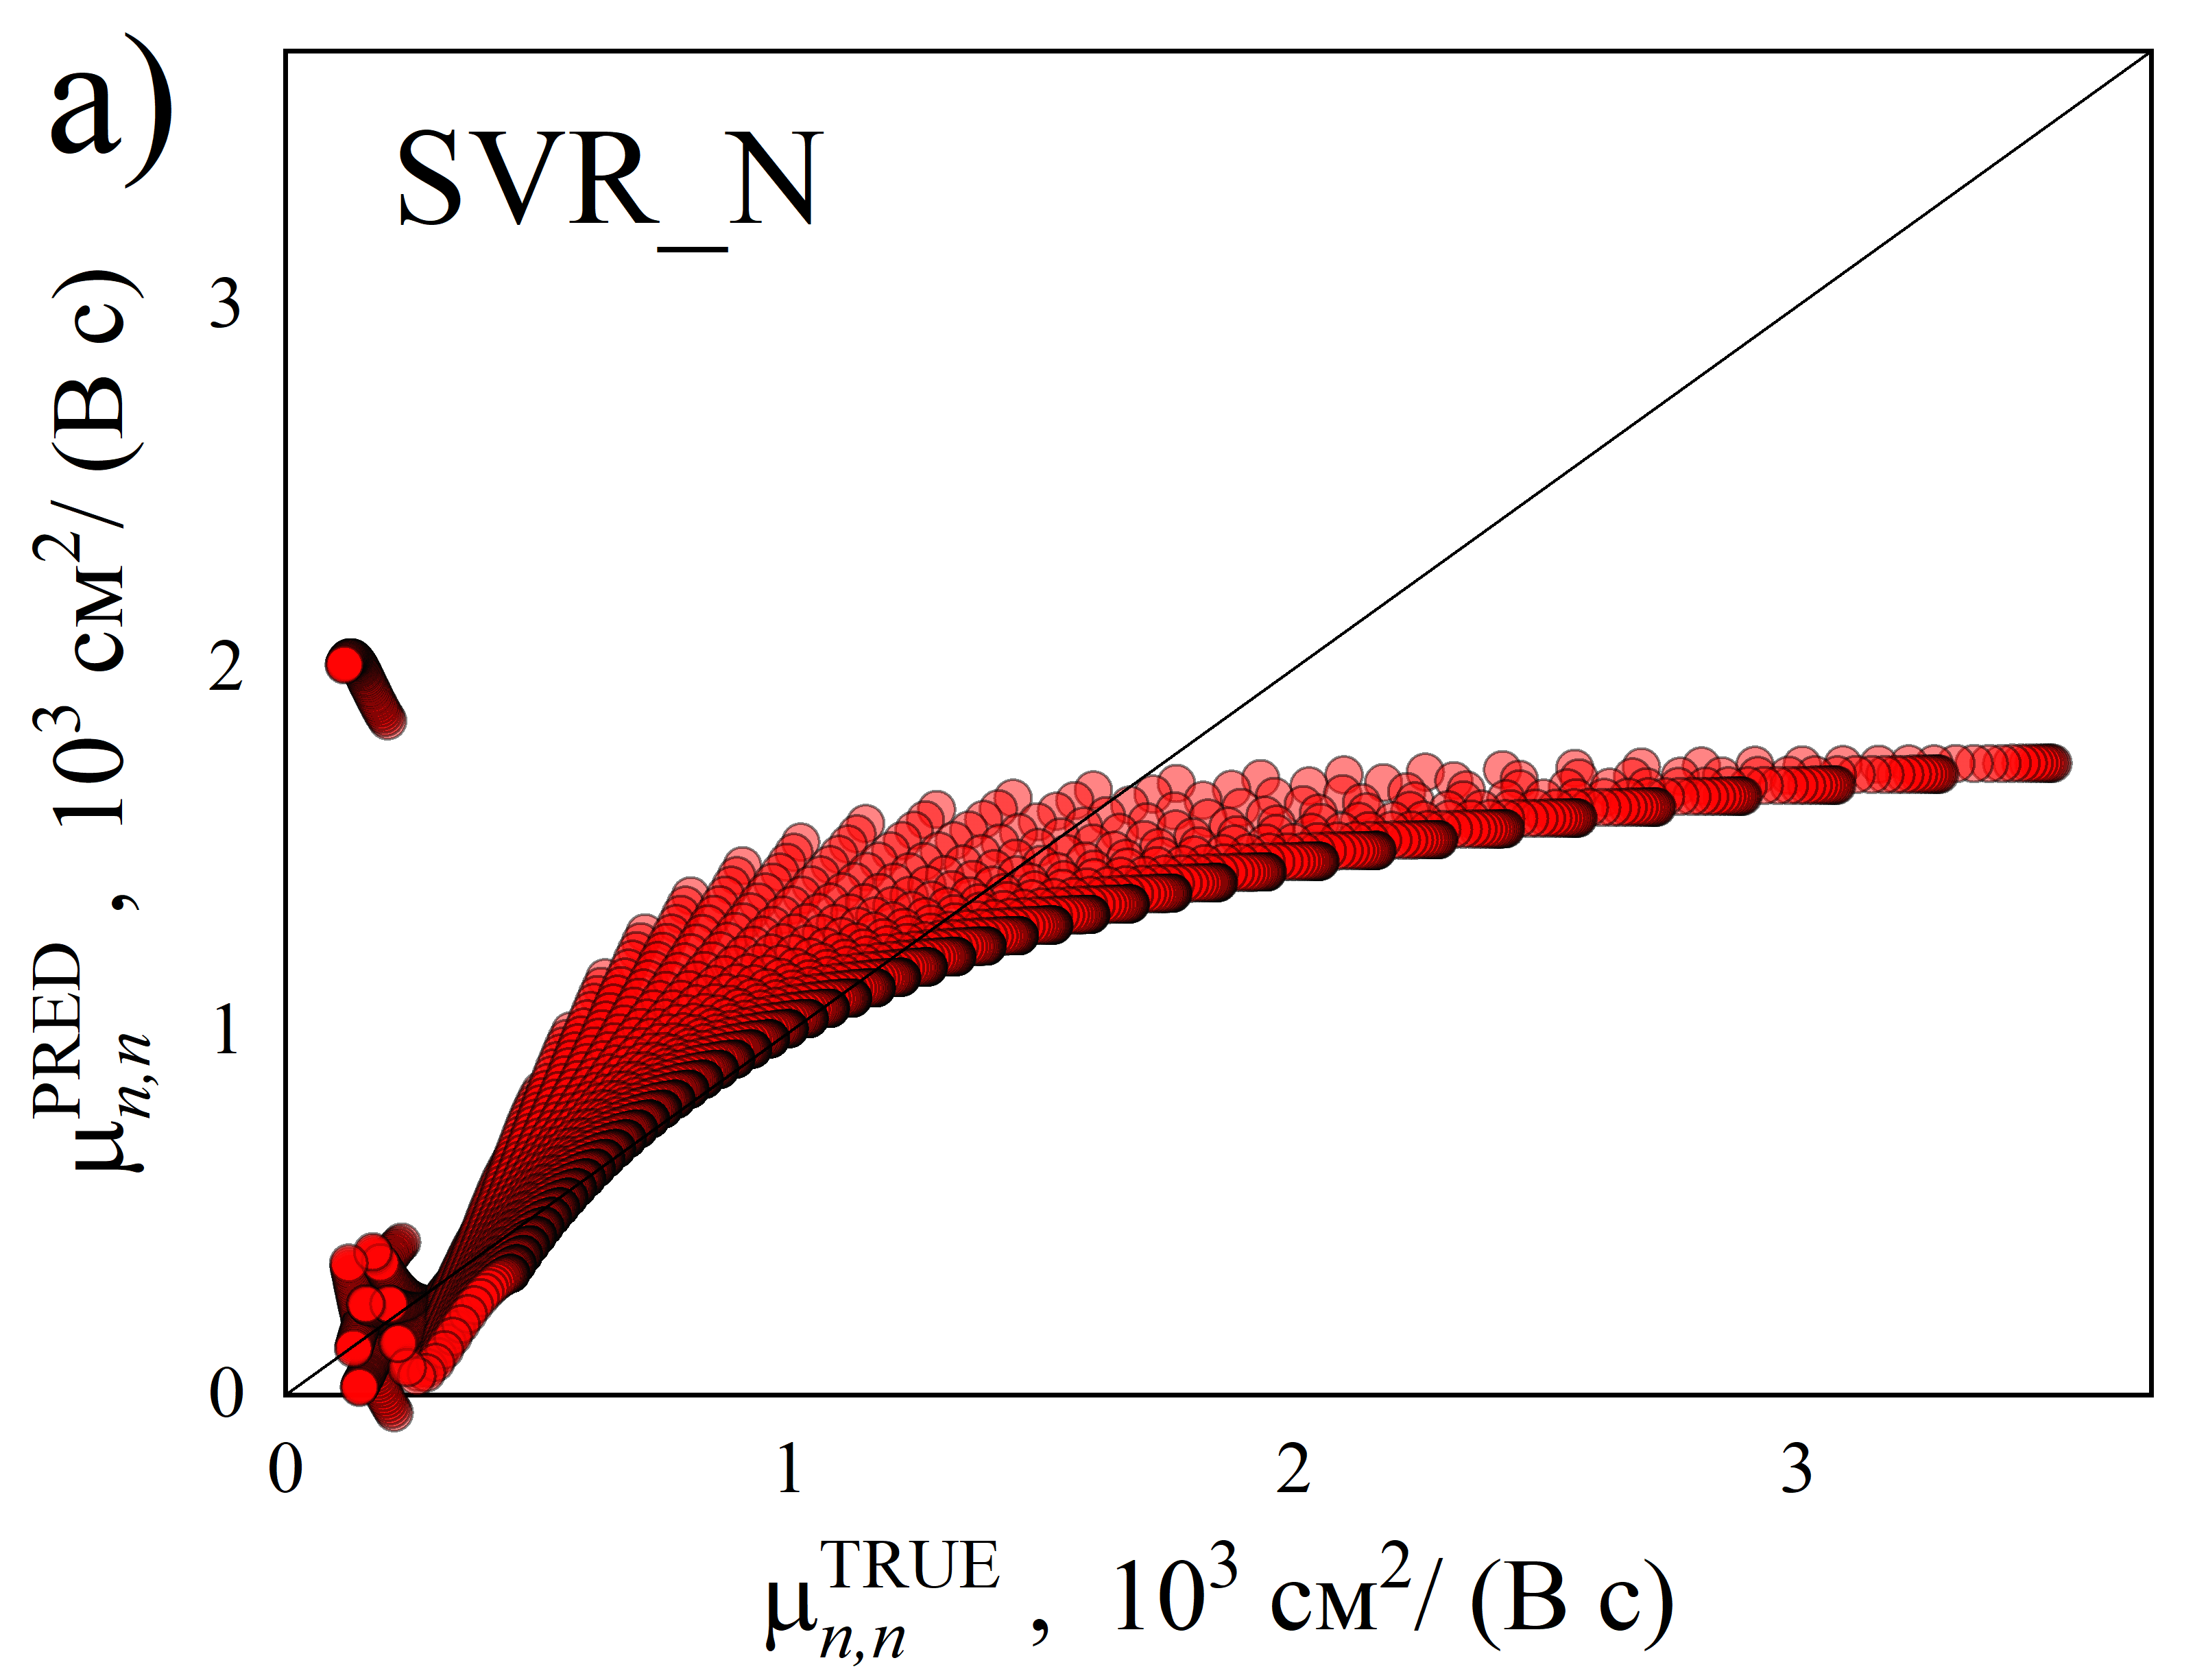
\includegraphics[width=0.35\linewidth]{SVRNnn.png}\kern 20pt
     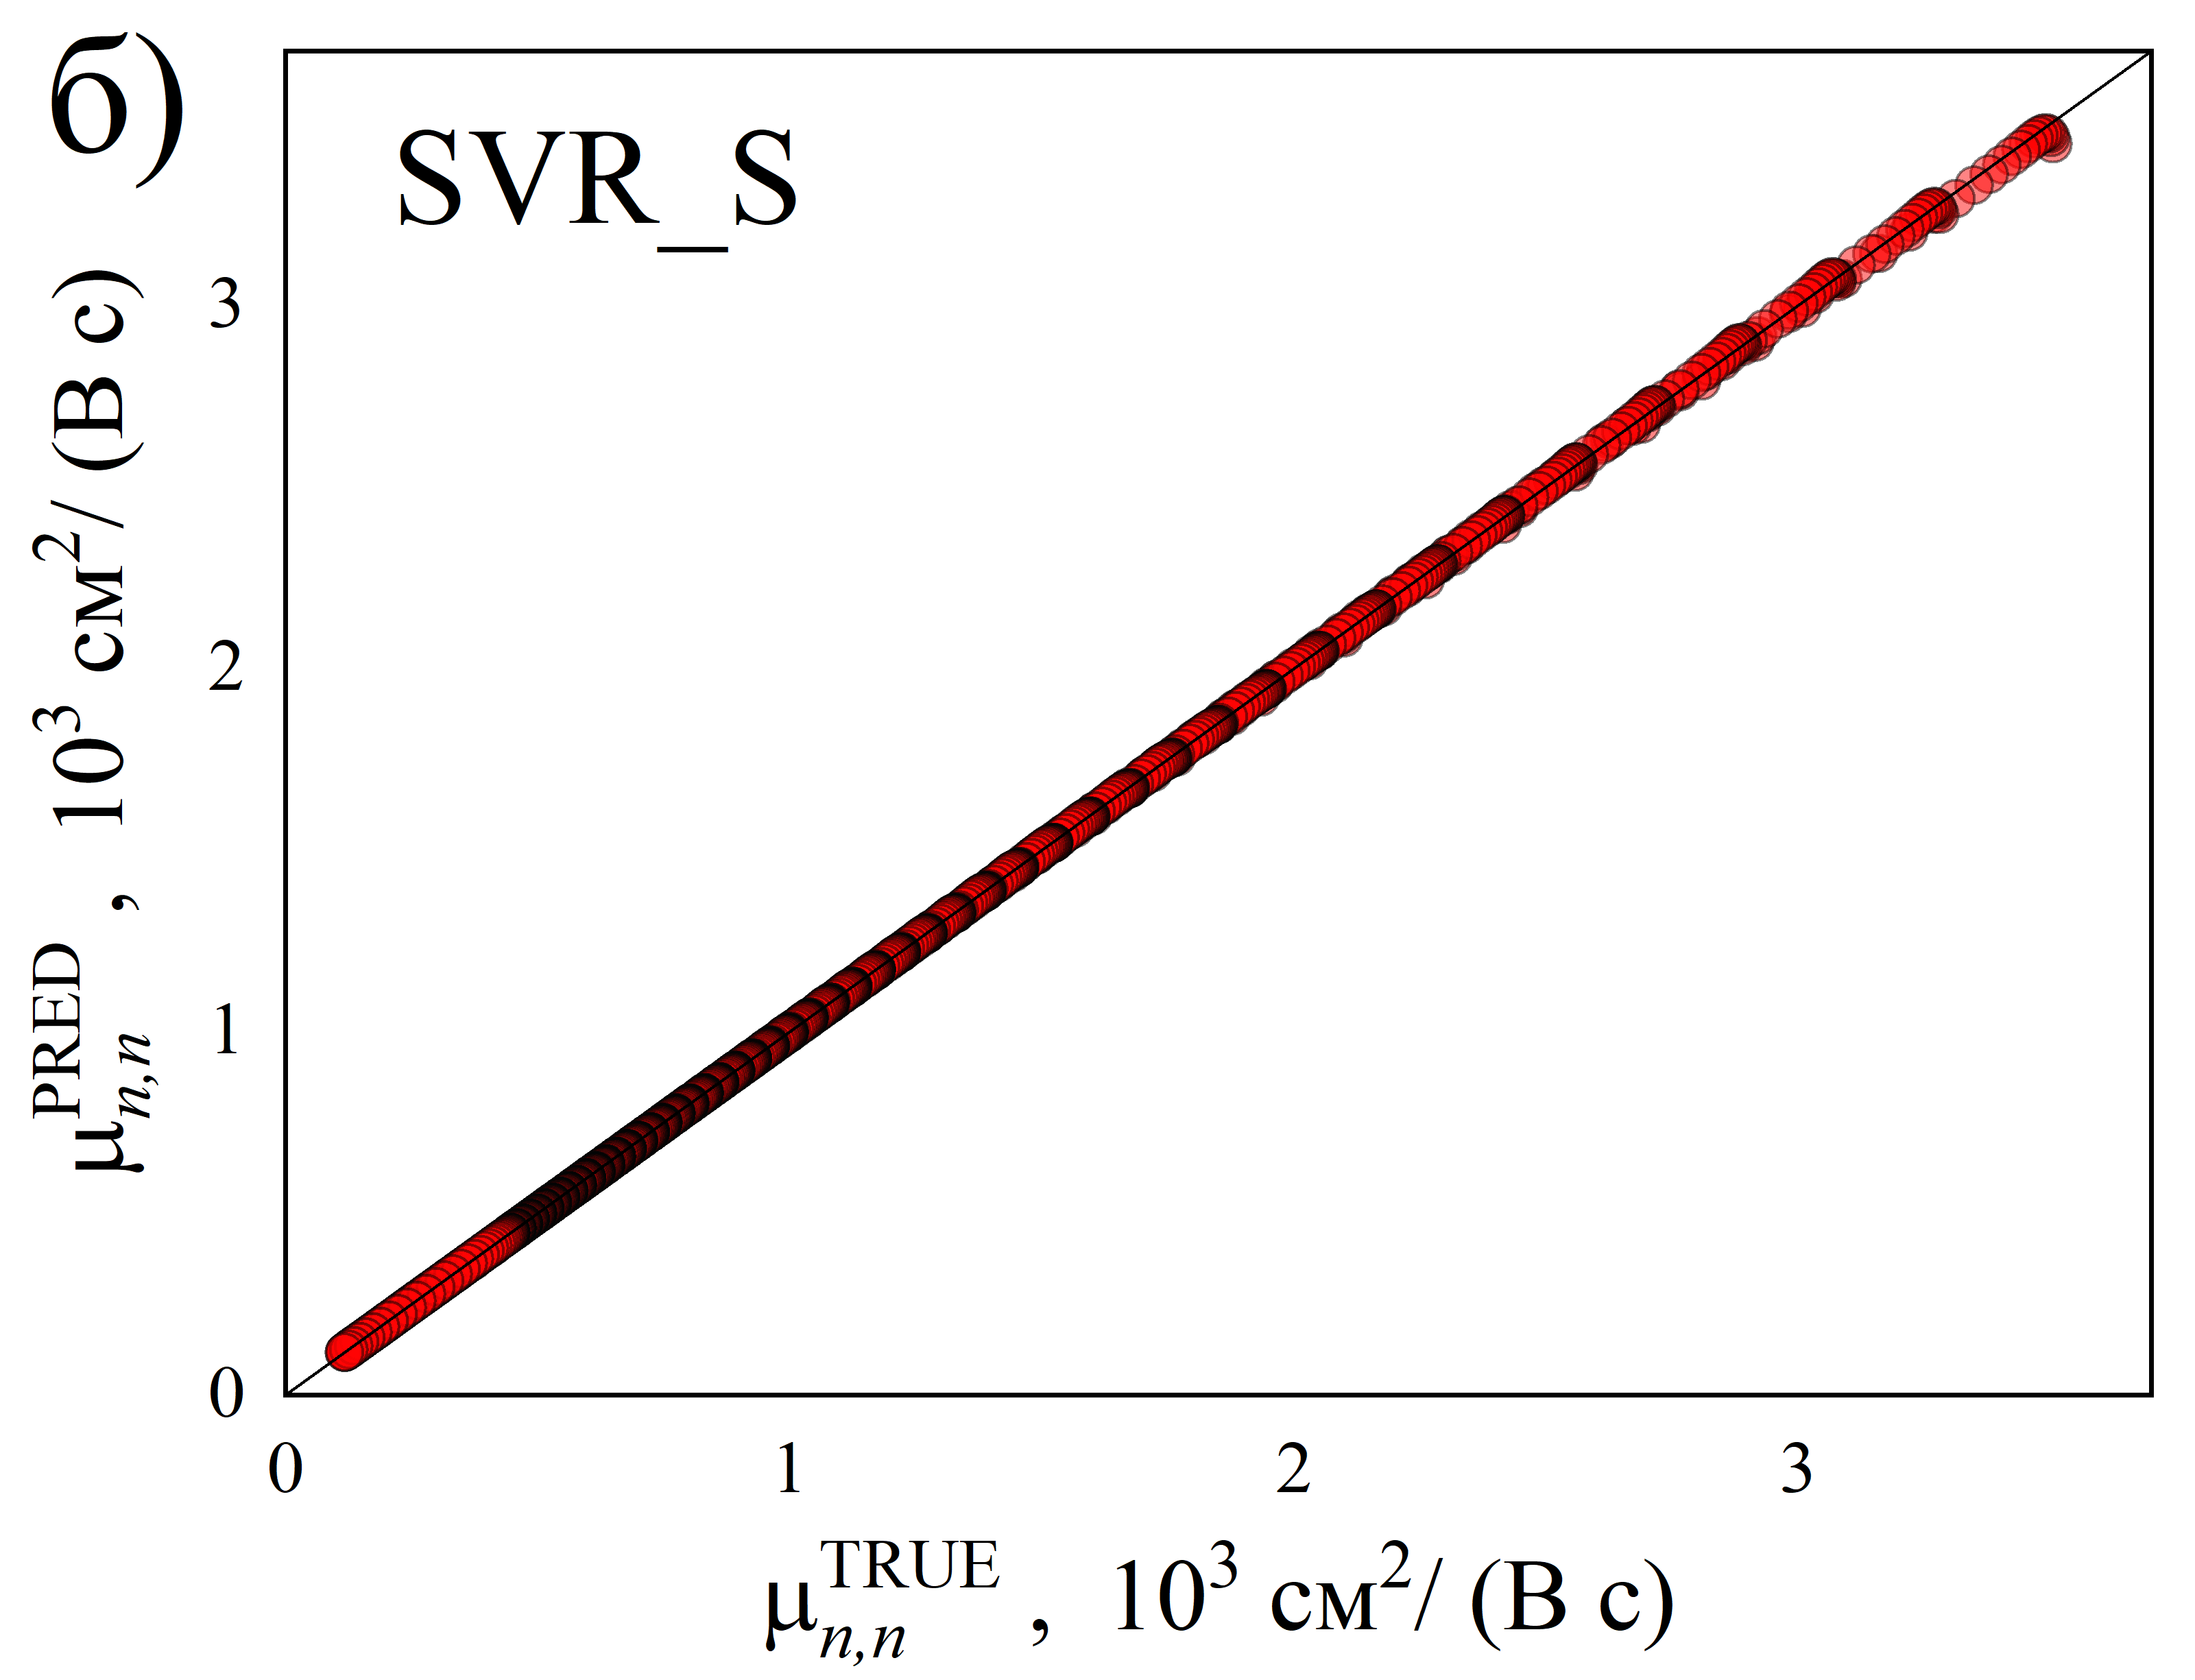
\includegraphics[width=0.35\linewidth]{SVRSnn.png}
     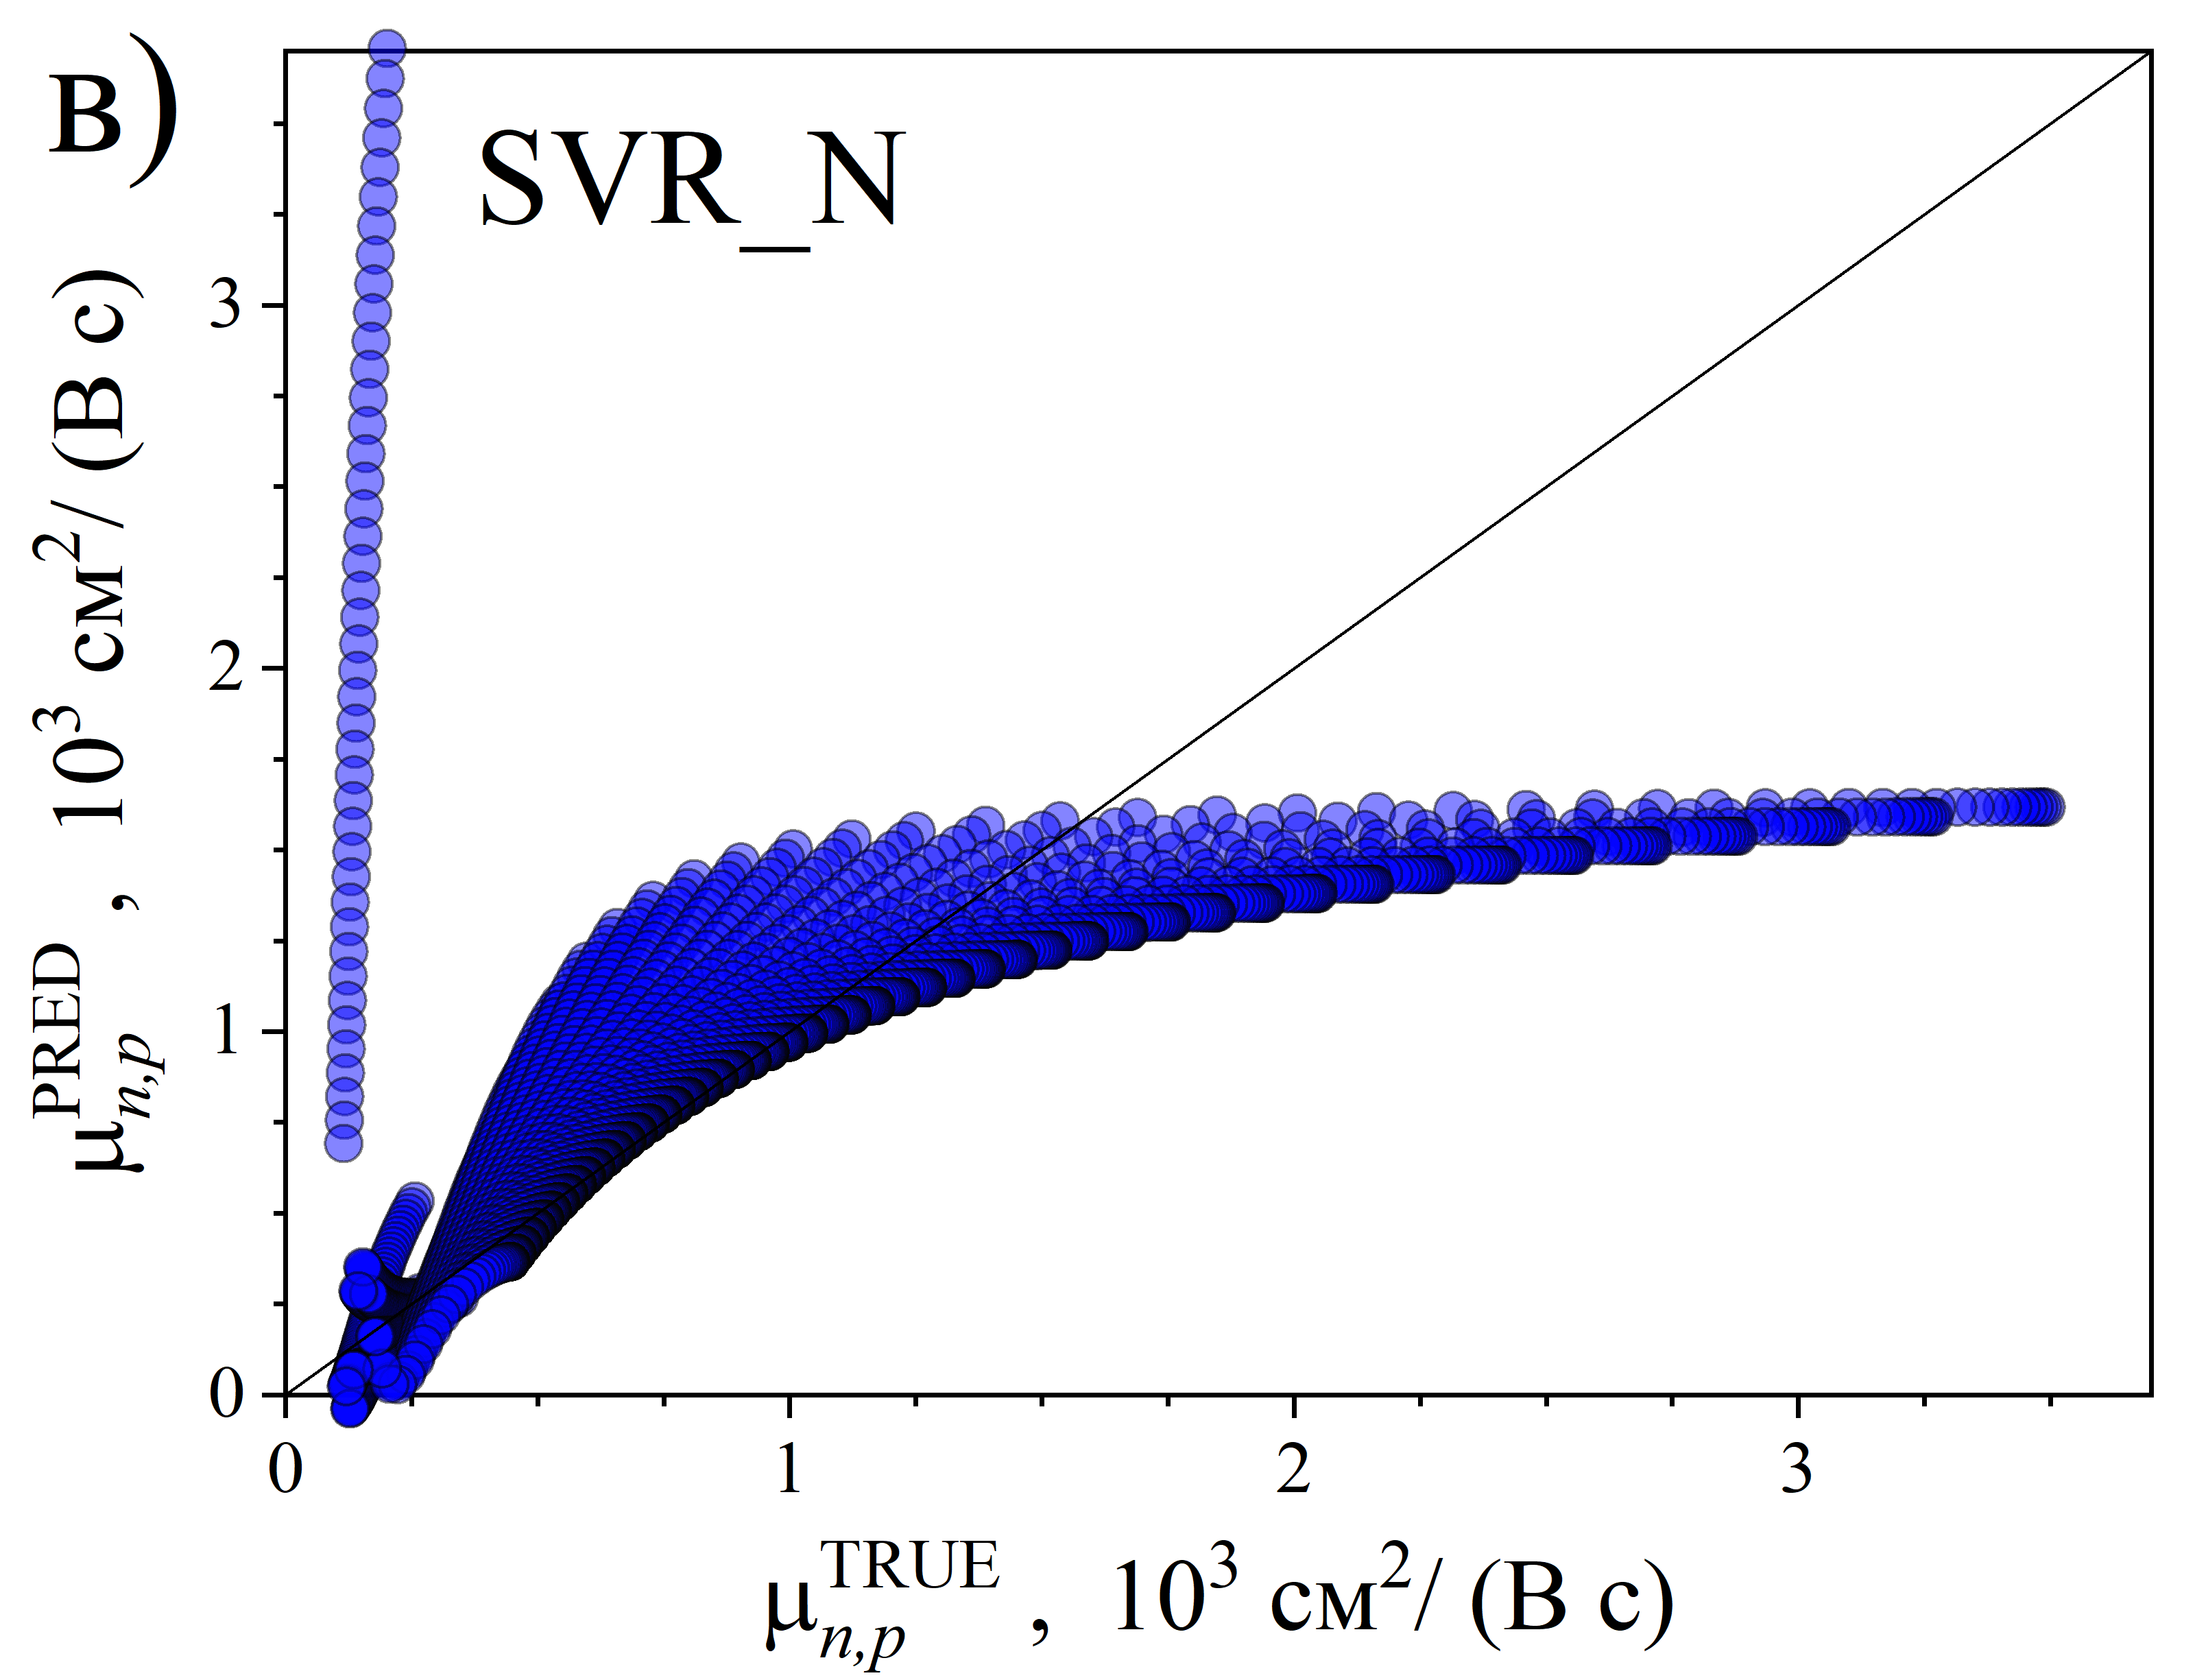
\includegraphics[width=0.35\linewidth]{SVRNnp.png}\kern 20pt
     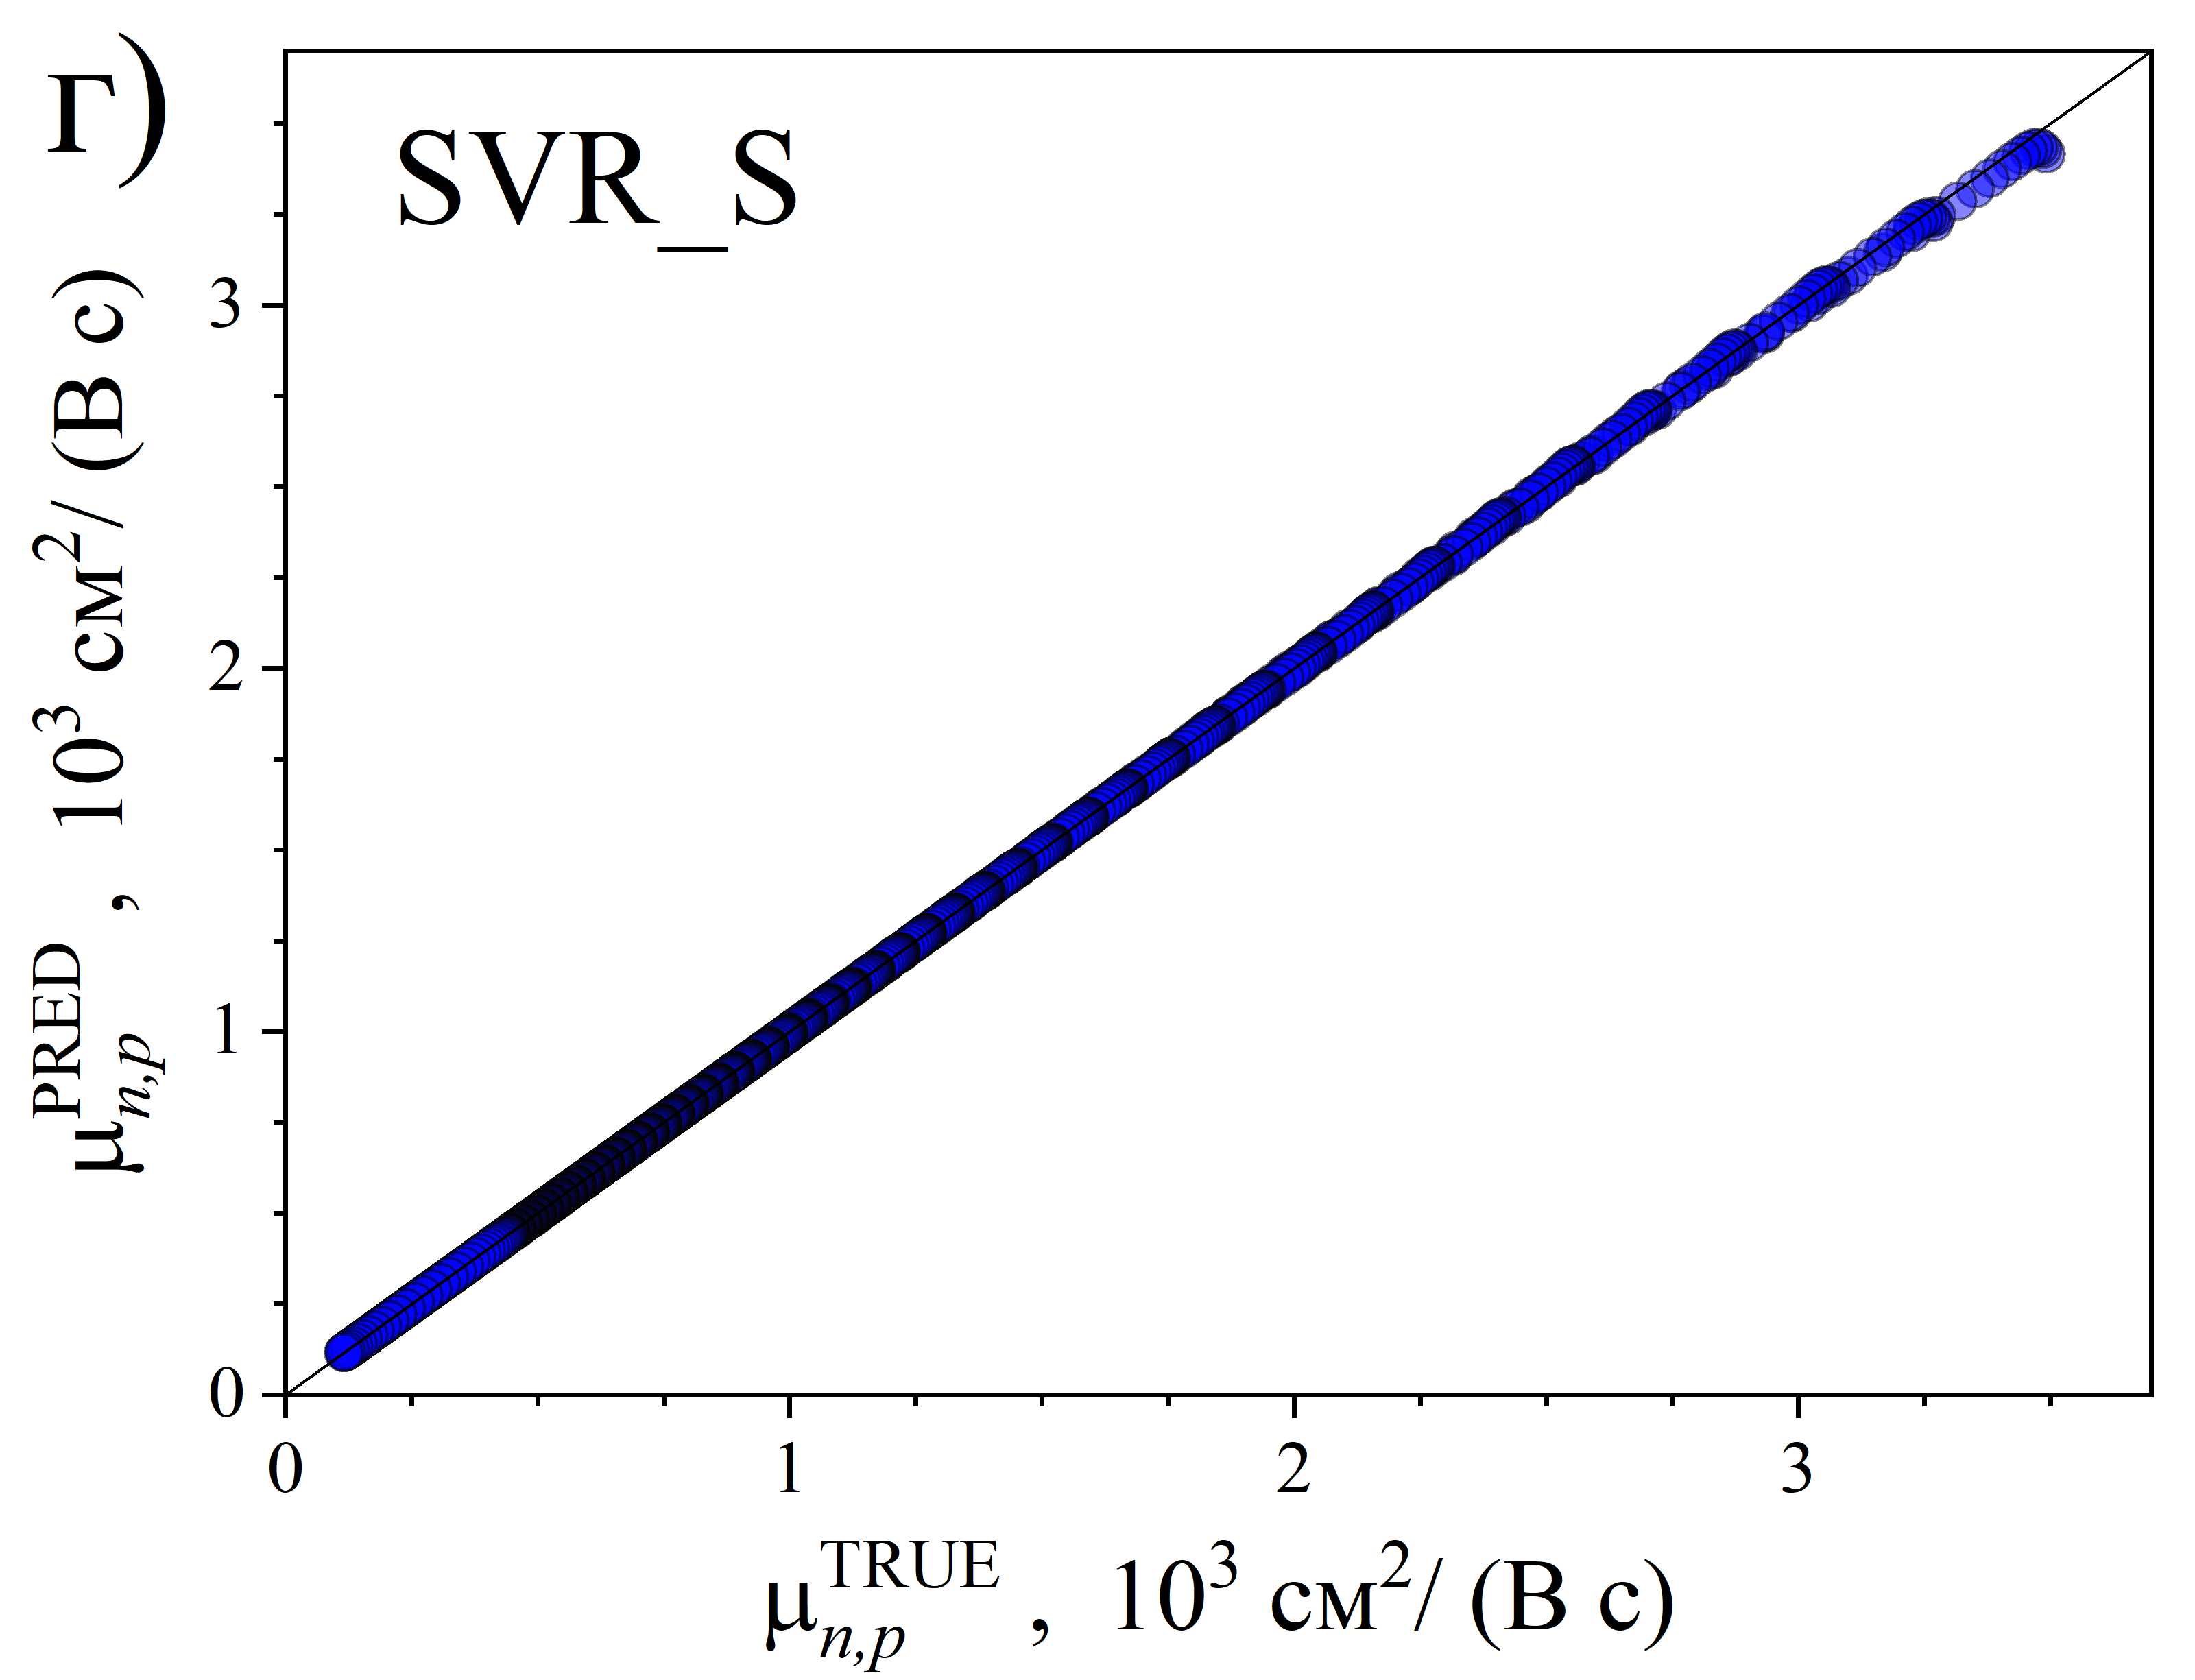
\includegraphics[width=0.35\linewidth]{SVRSnp.png}
     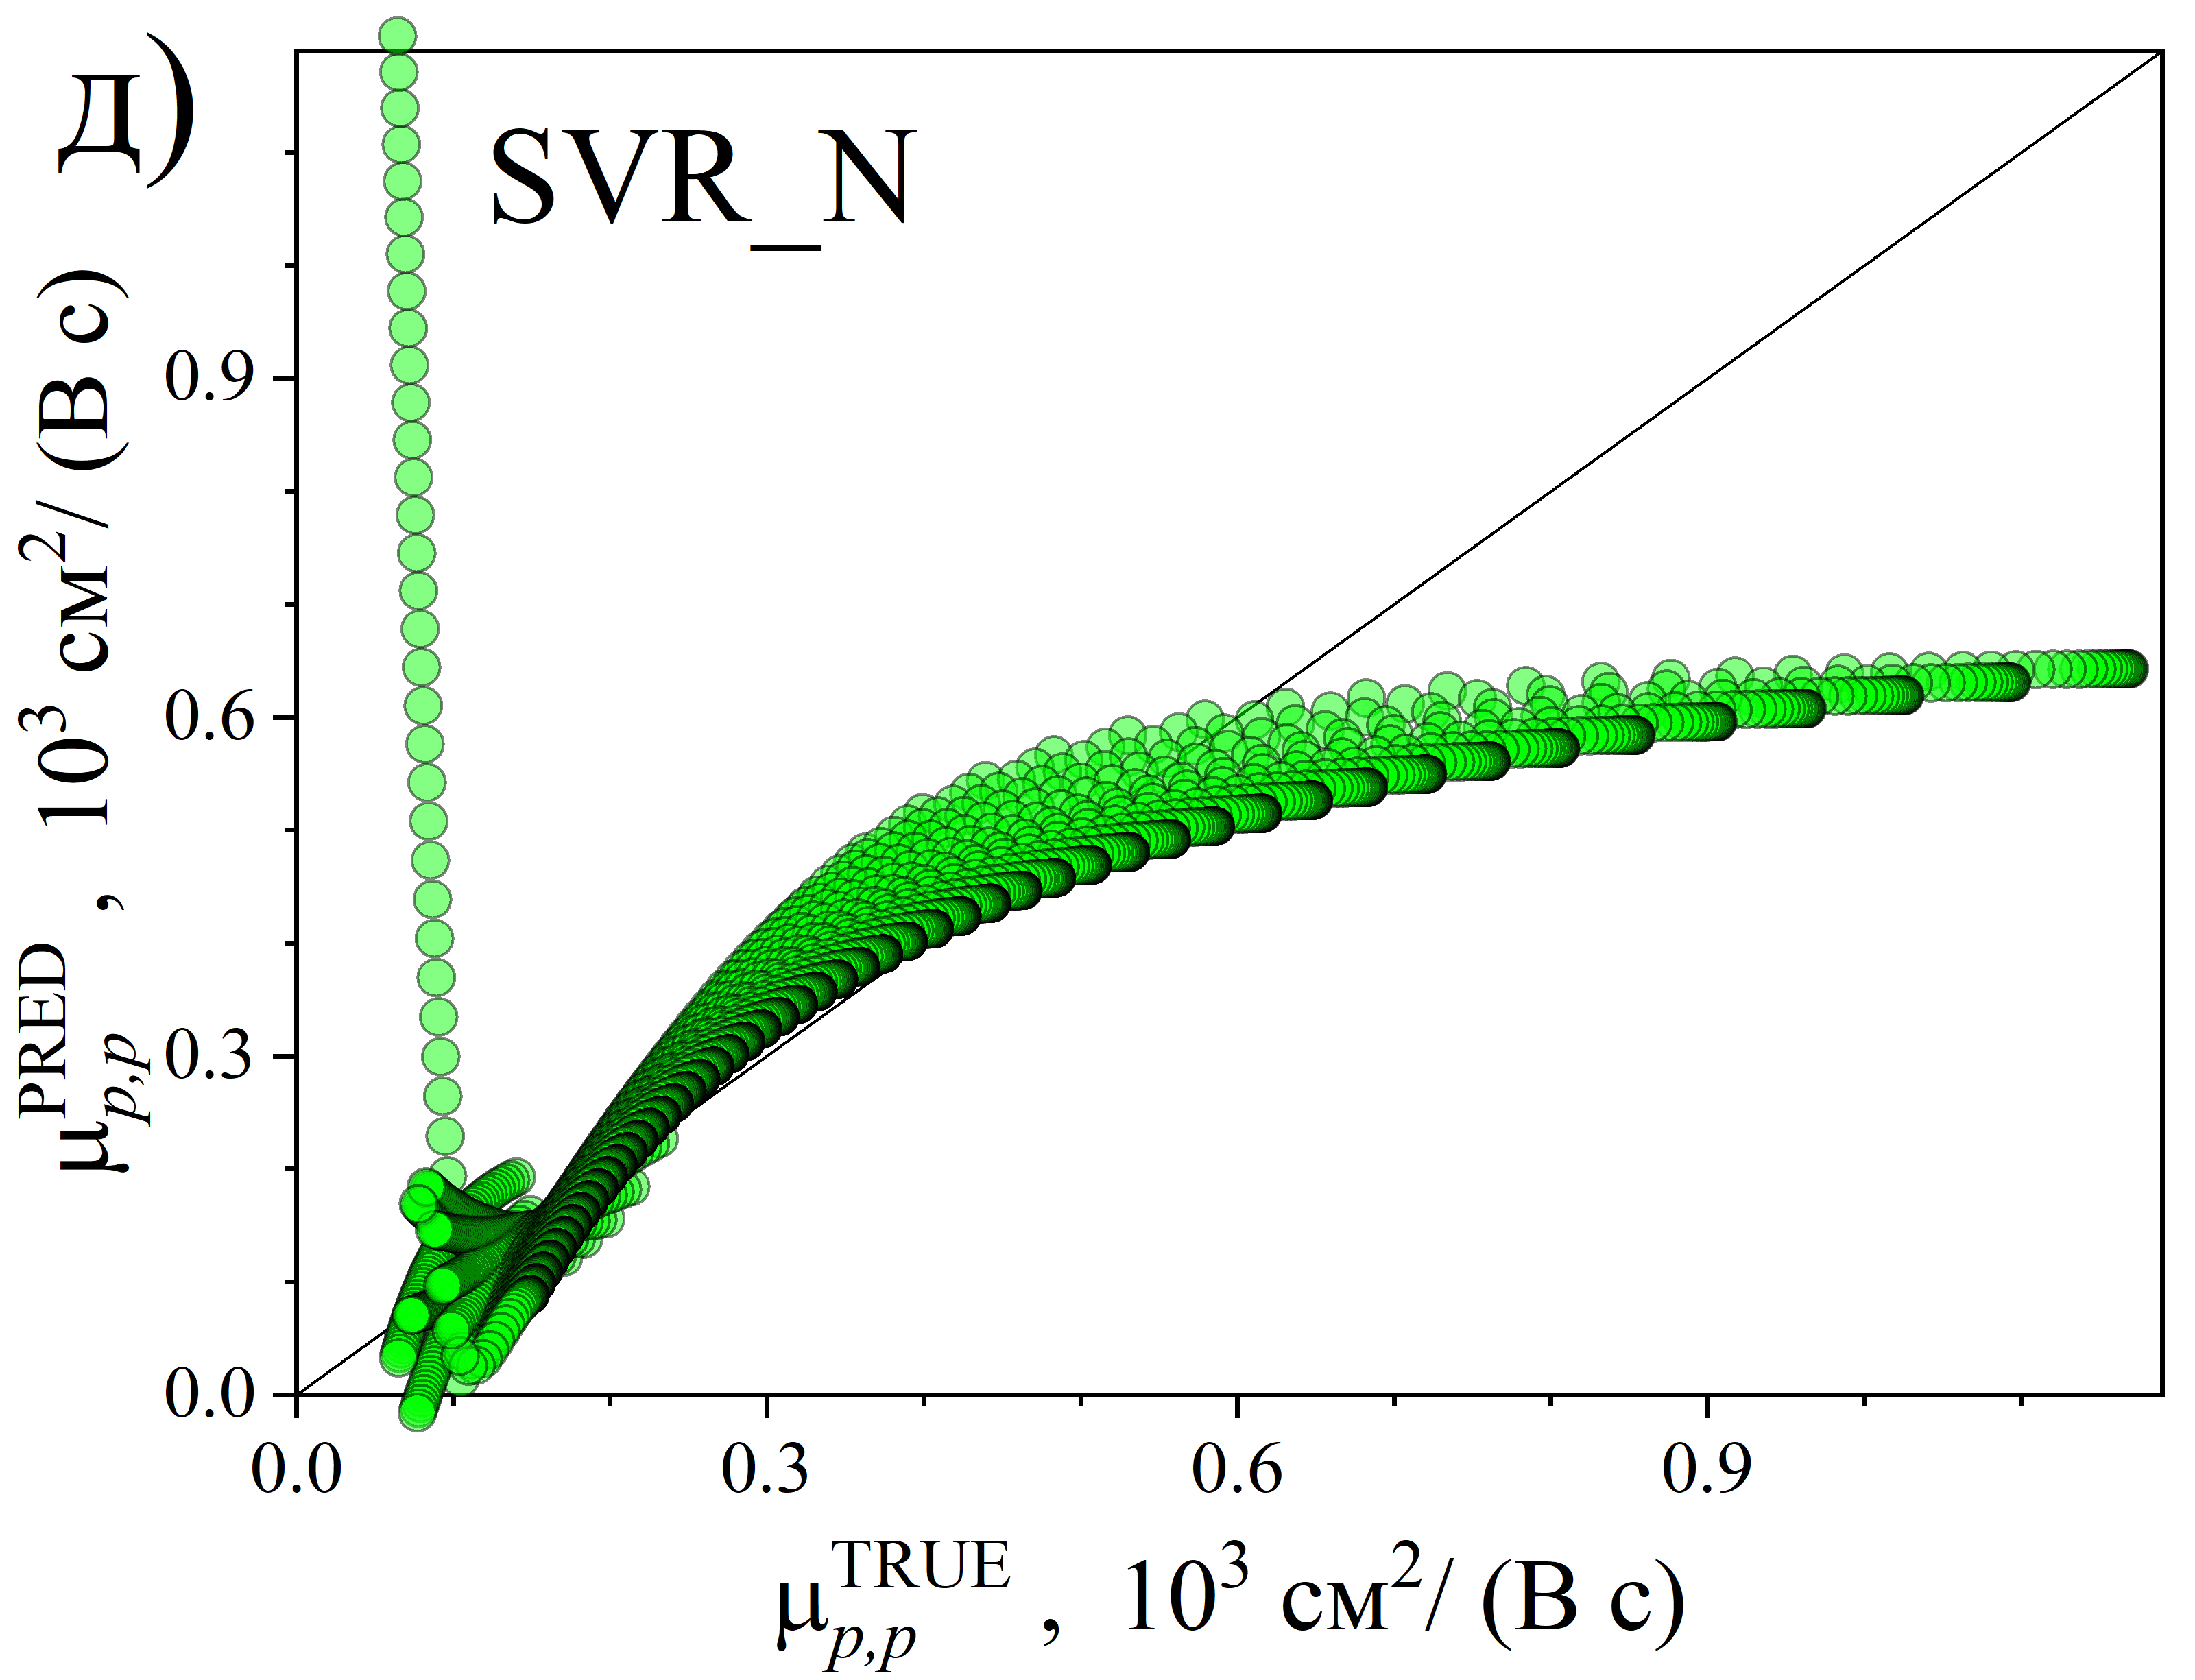
\includegraphics[width=0.35\linewidth]{SVRNpp.png}\kern 20pt
     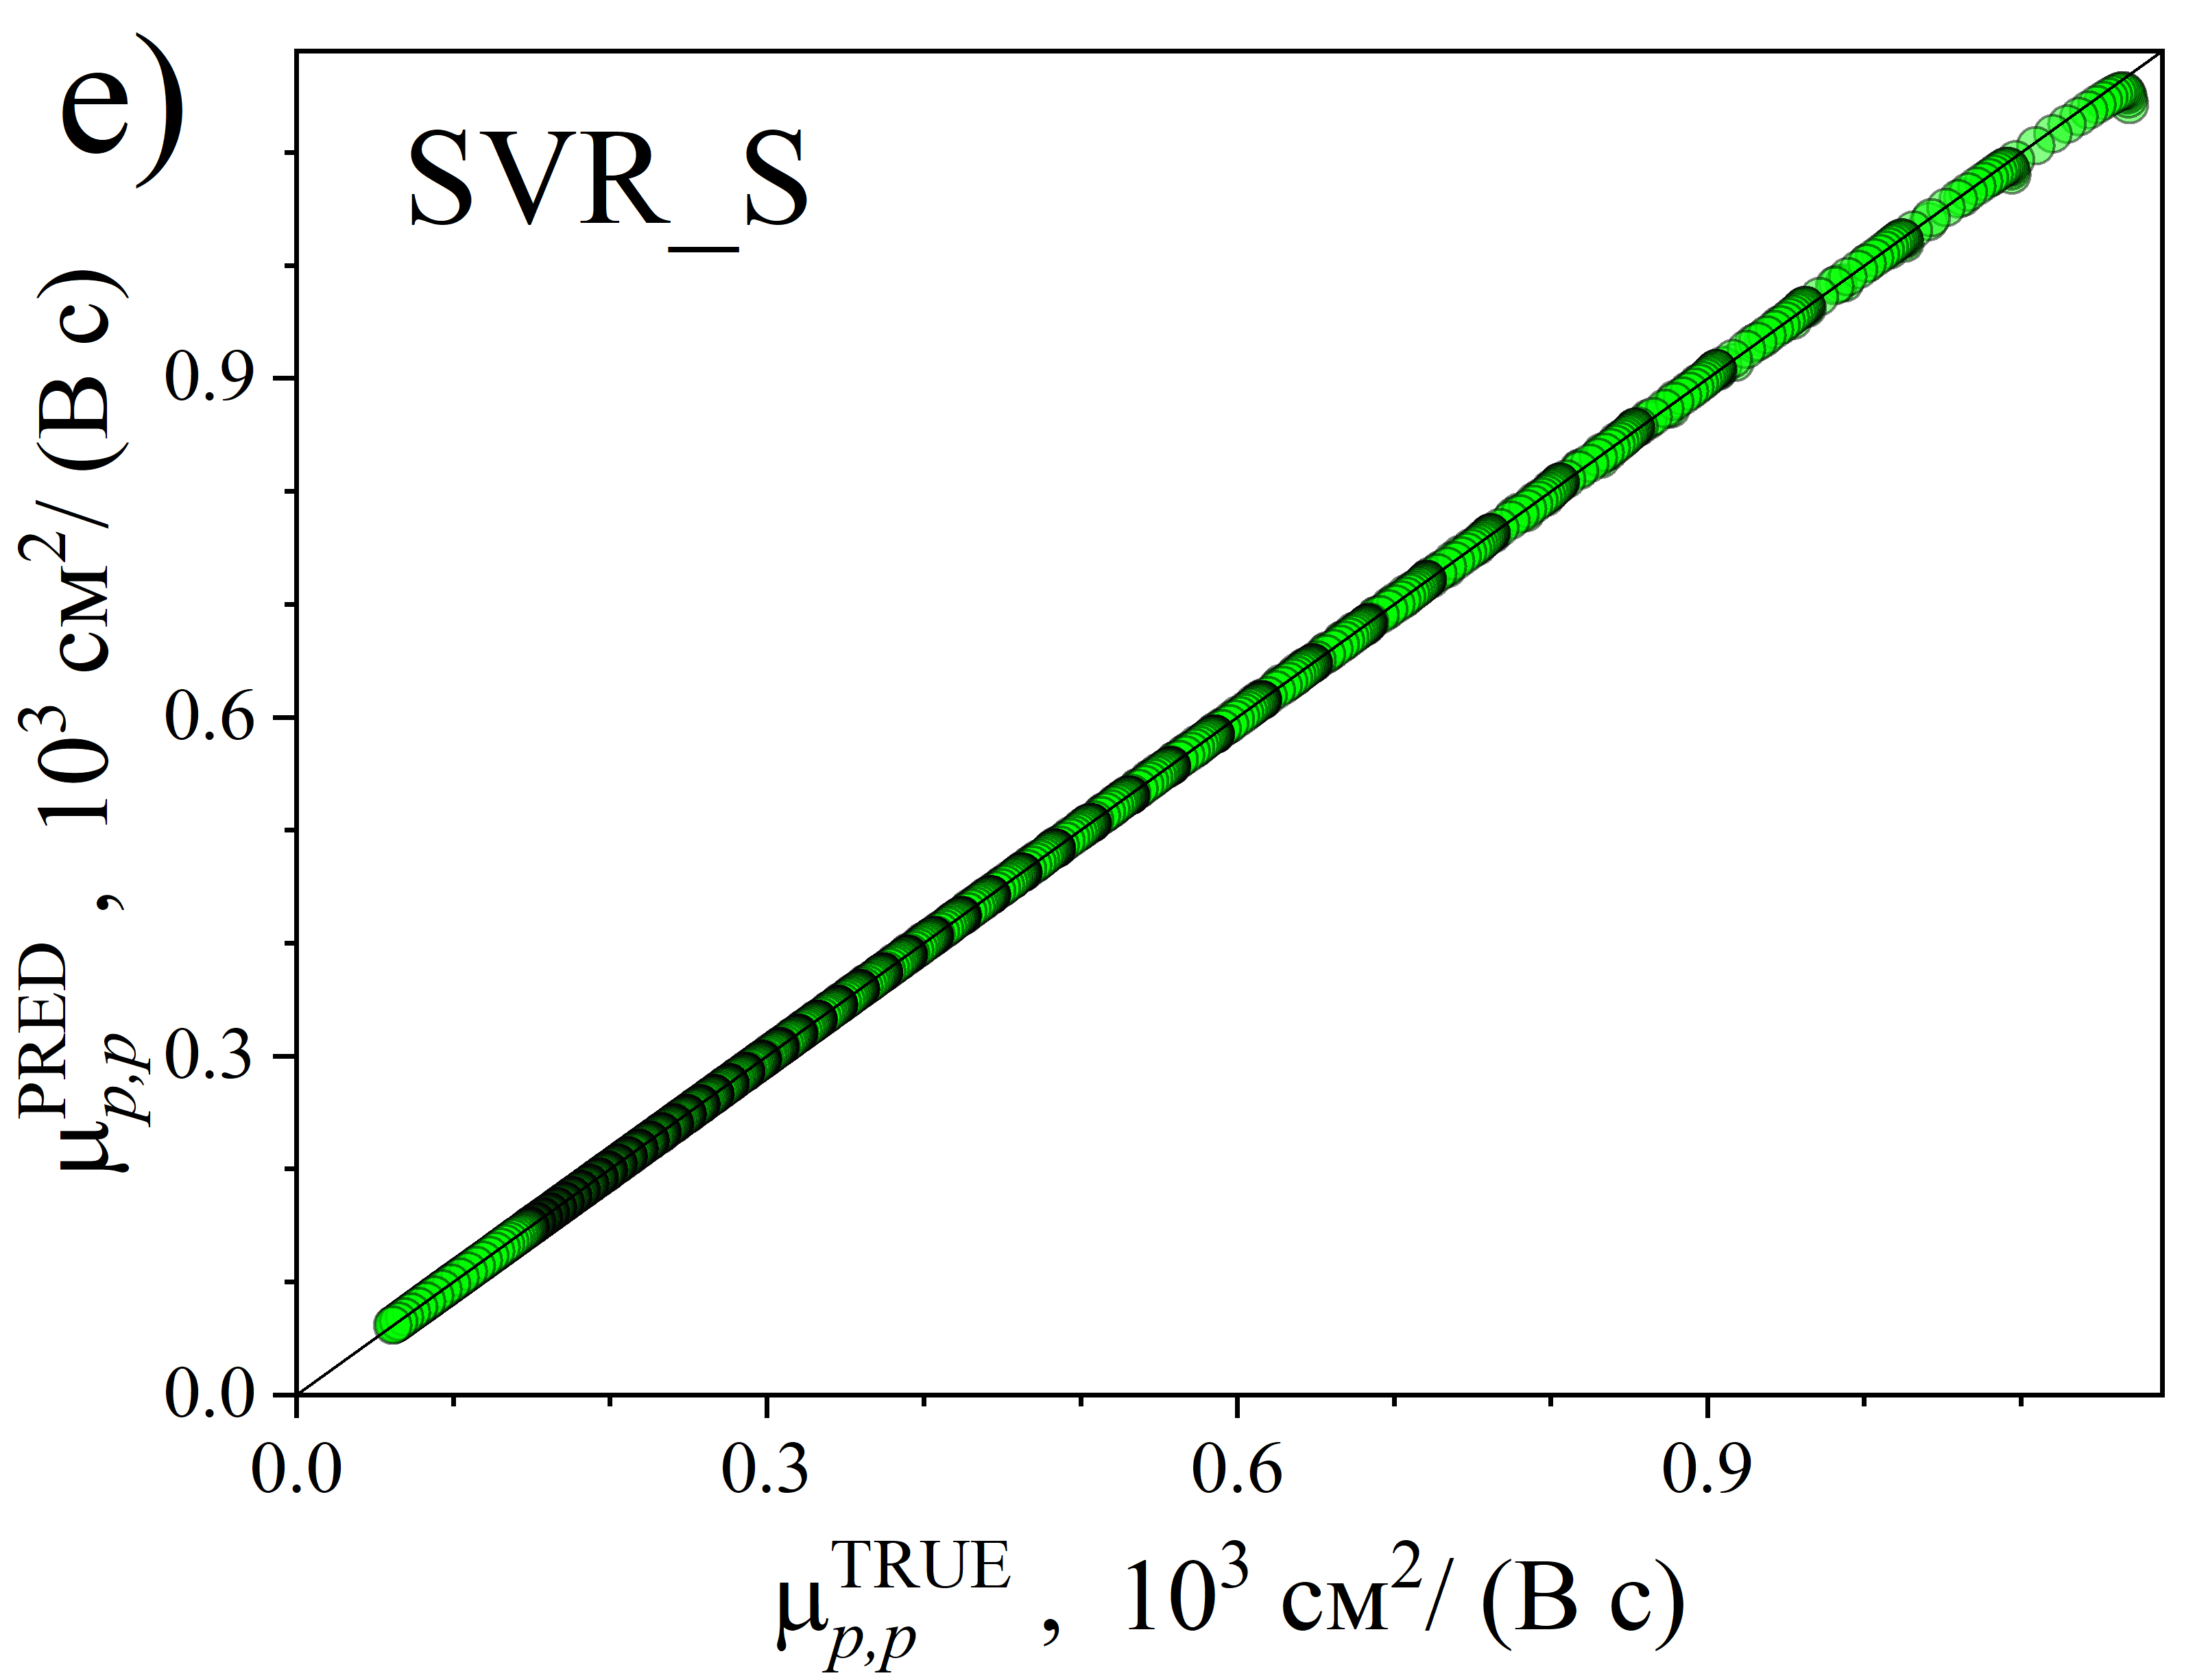
\includegraphics[width=0.35\linewidth]{SVRSpp.png}
     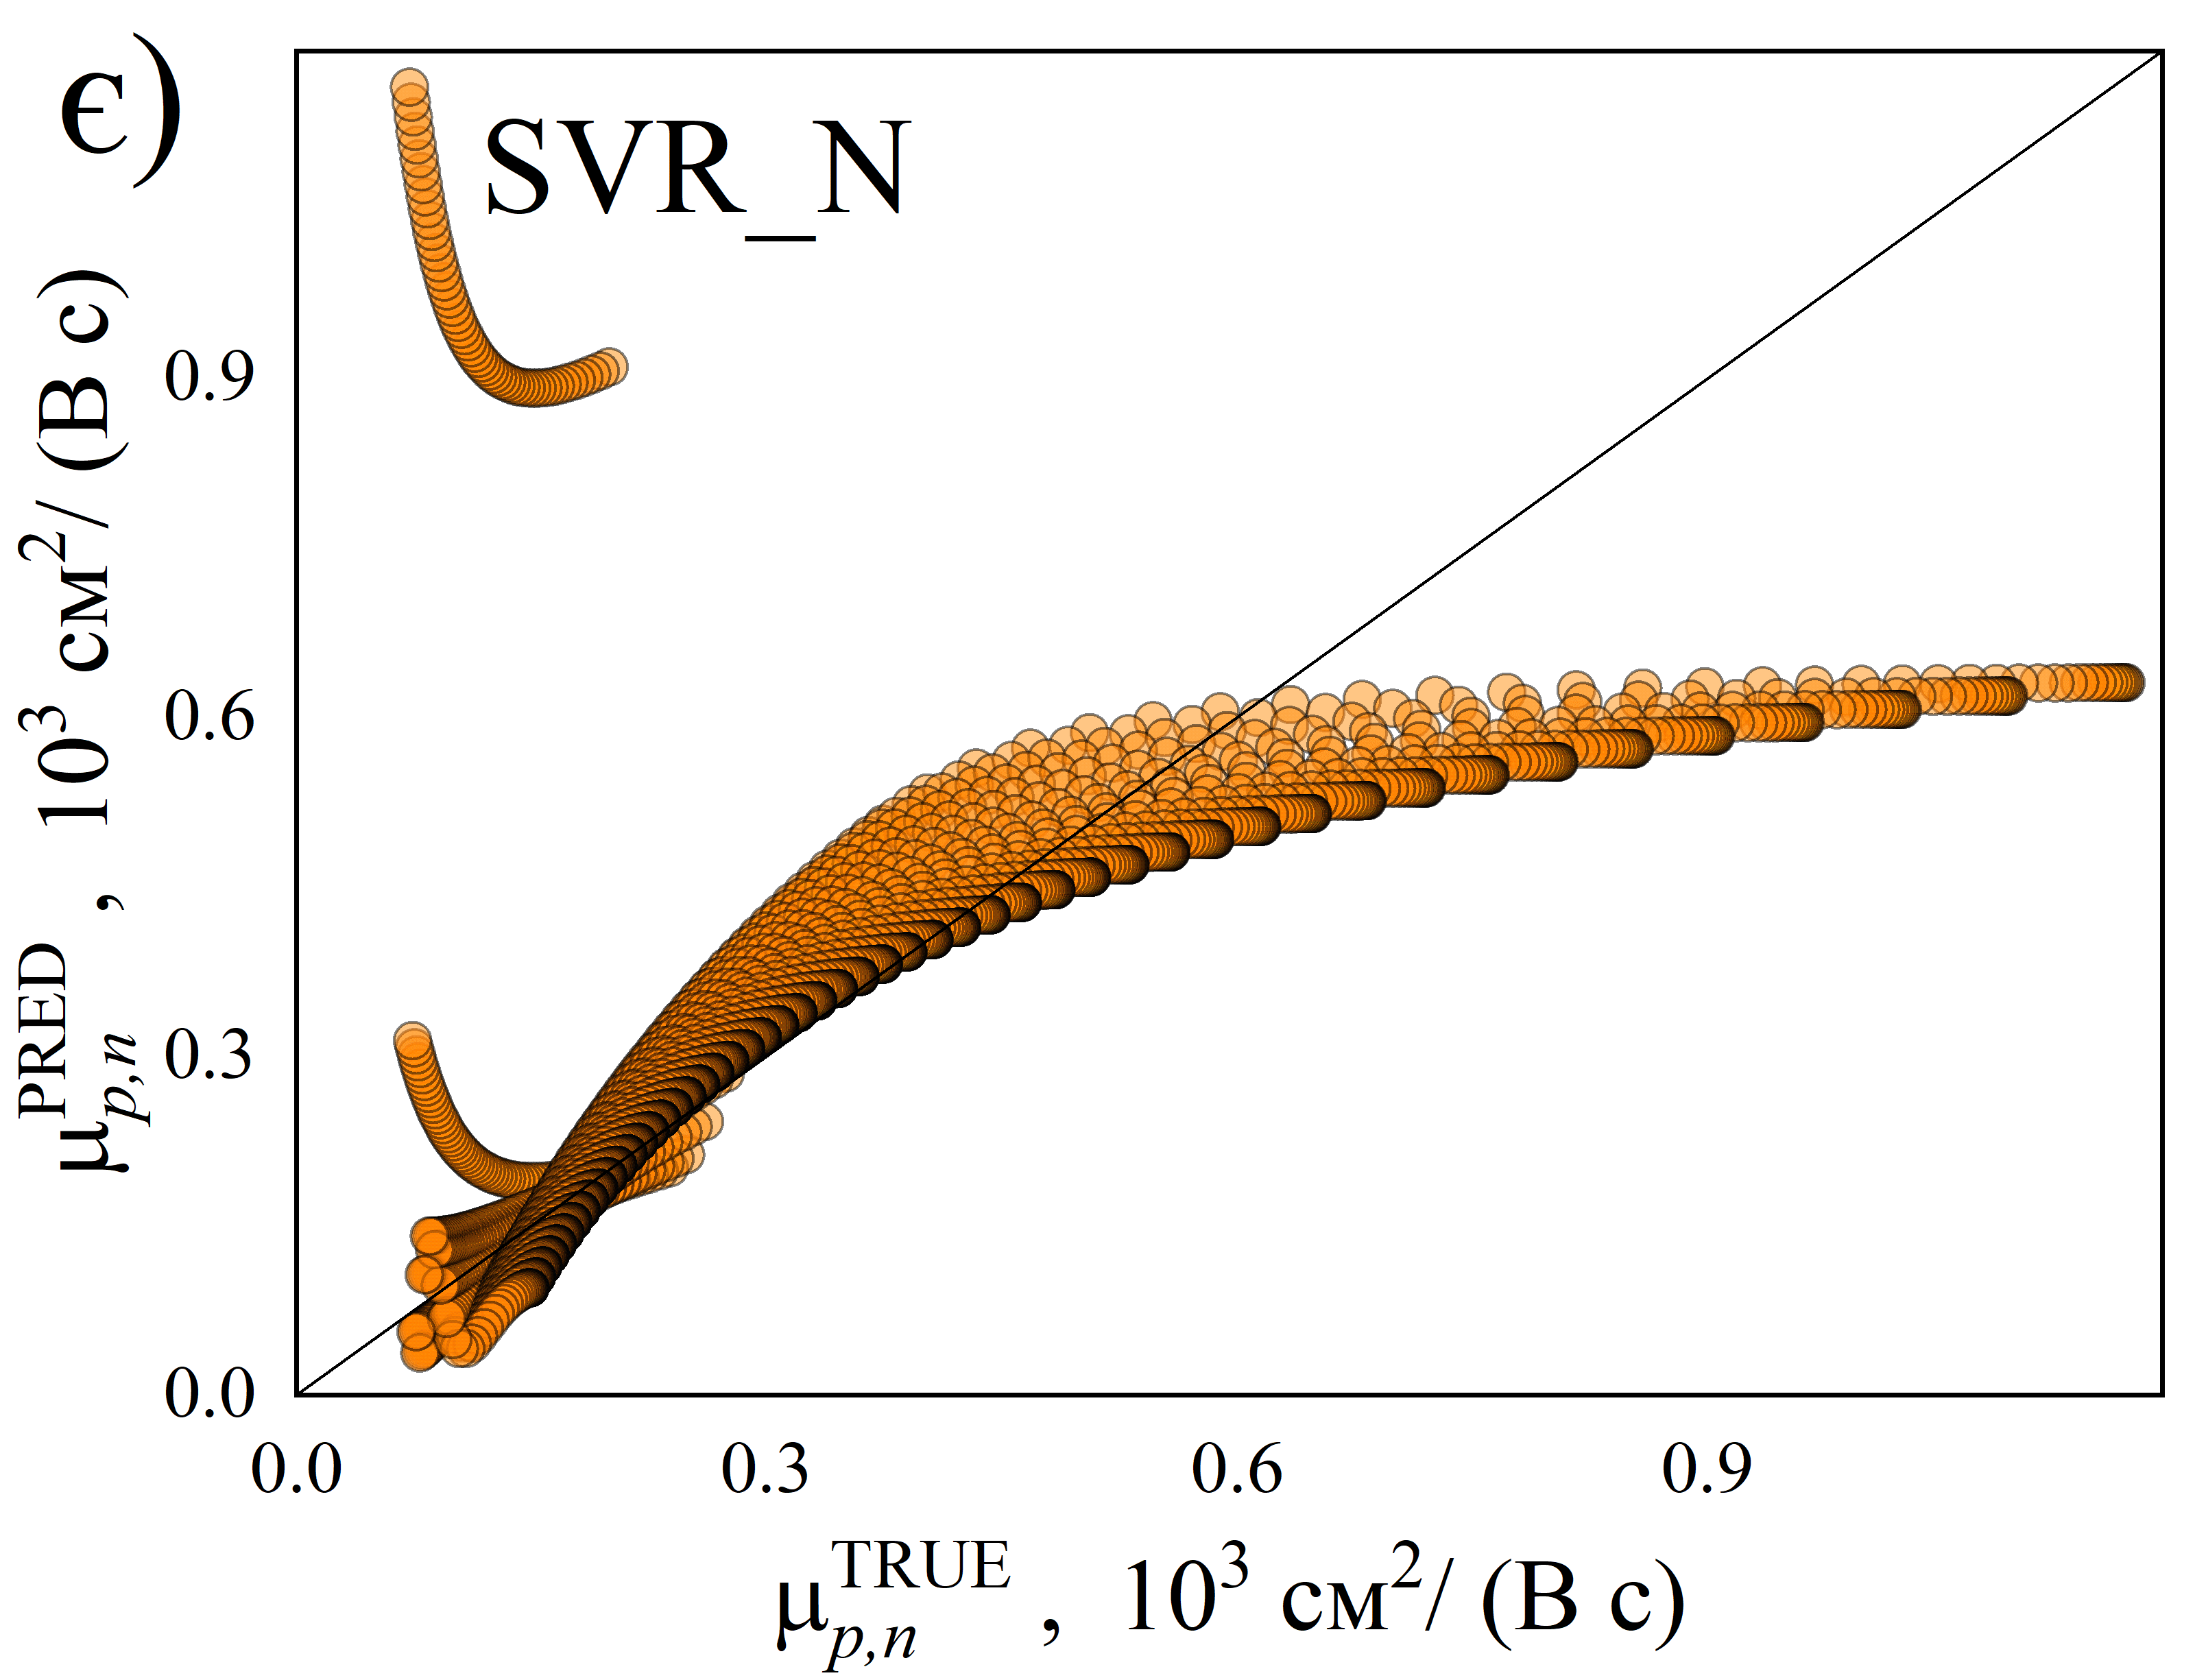
\includegraphics[width=0.35\linewidth]{SVRNpn.png}\kern 20pt
     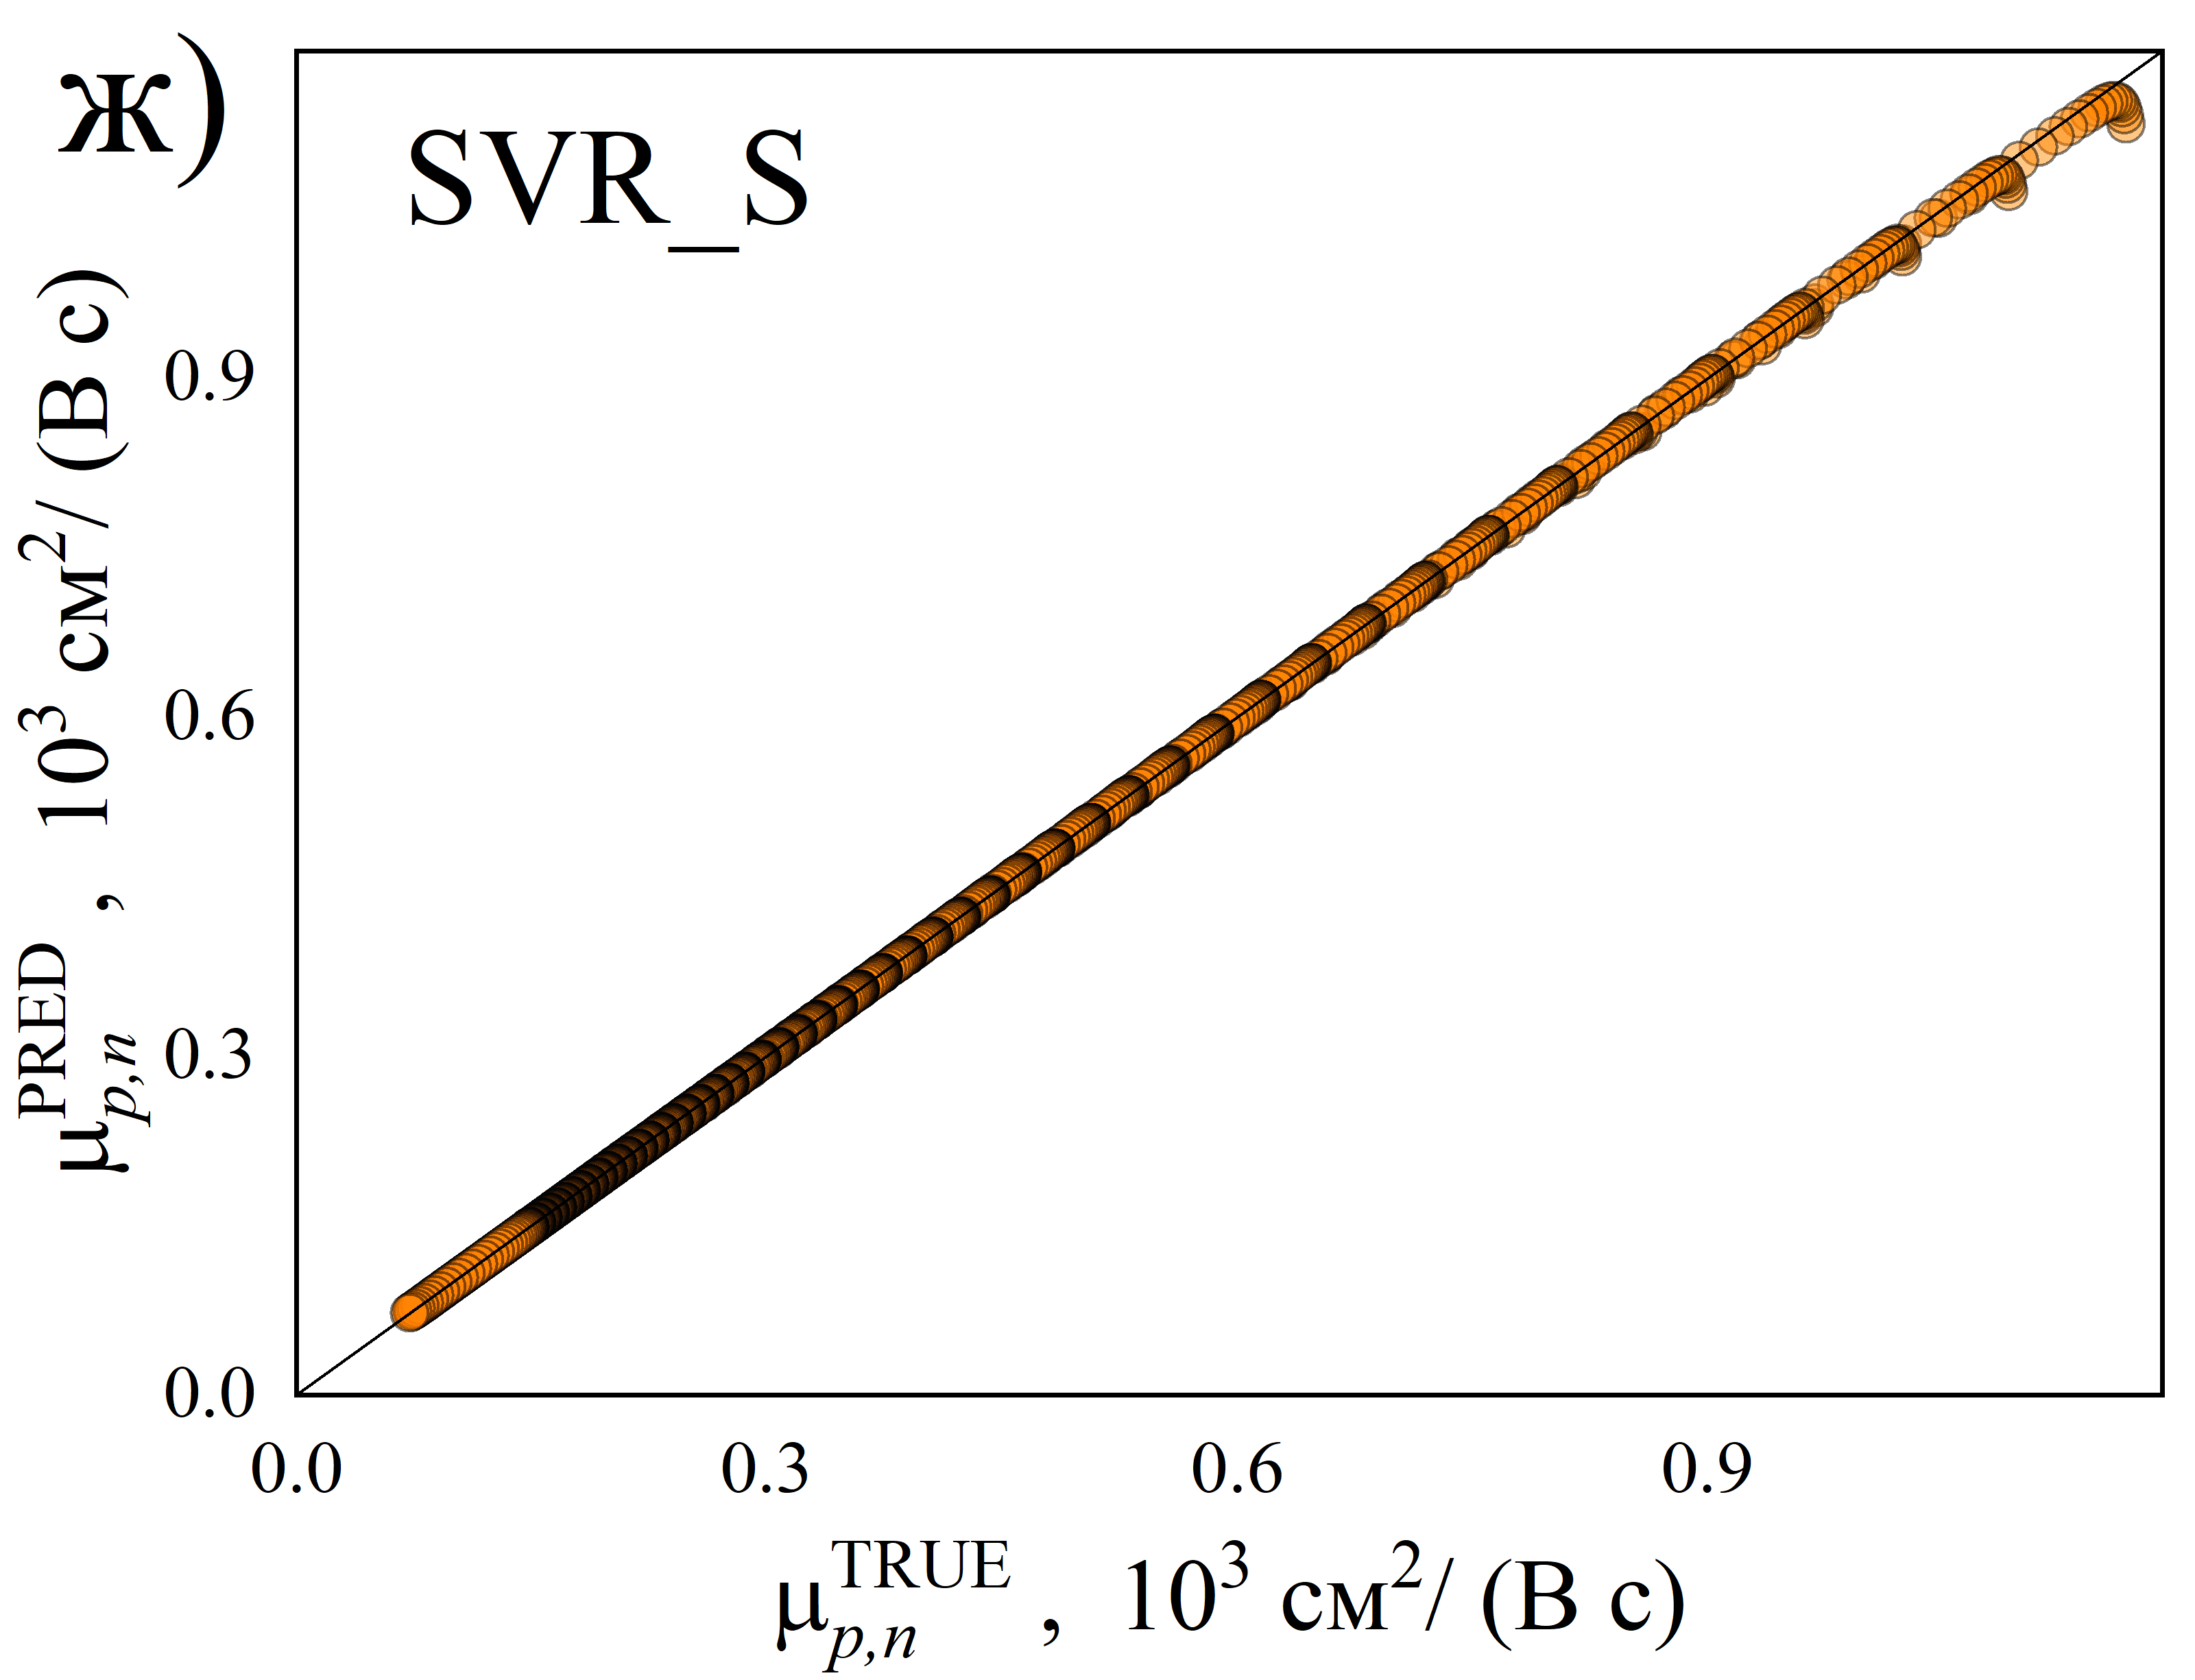
\includegraphics[width=0.35\linewidth]{SVRSpn.png}
	  \caption{Діаграми розсіювання, що порівнюють еталонні значення рухливості із значеннями, передбаченими SVR моделями
       на тестовому наборі даних.
       Представлені випадки оцінки рухливості електронів (а--г) та дірок (д--ж), коли вони є
       основними (а, б, д, е) та неосновними (в, г, є, ж) носіями заряду.
       Попередня підготовка даних передбачала нормування (а, в, д, є) або нормалізацію (б, г, е, ж).
}\label{figSVR}
\end{figure}



\begin{figure}
	\centering
     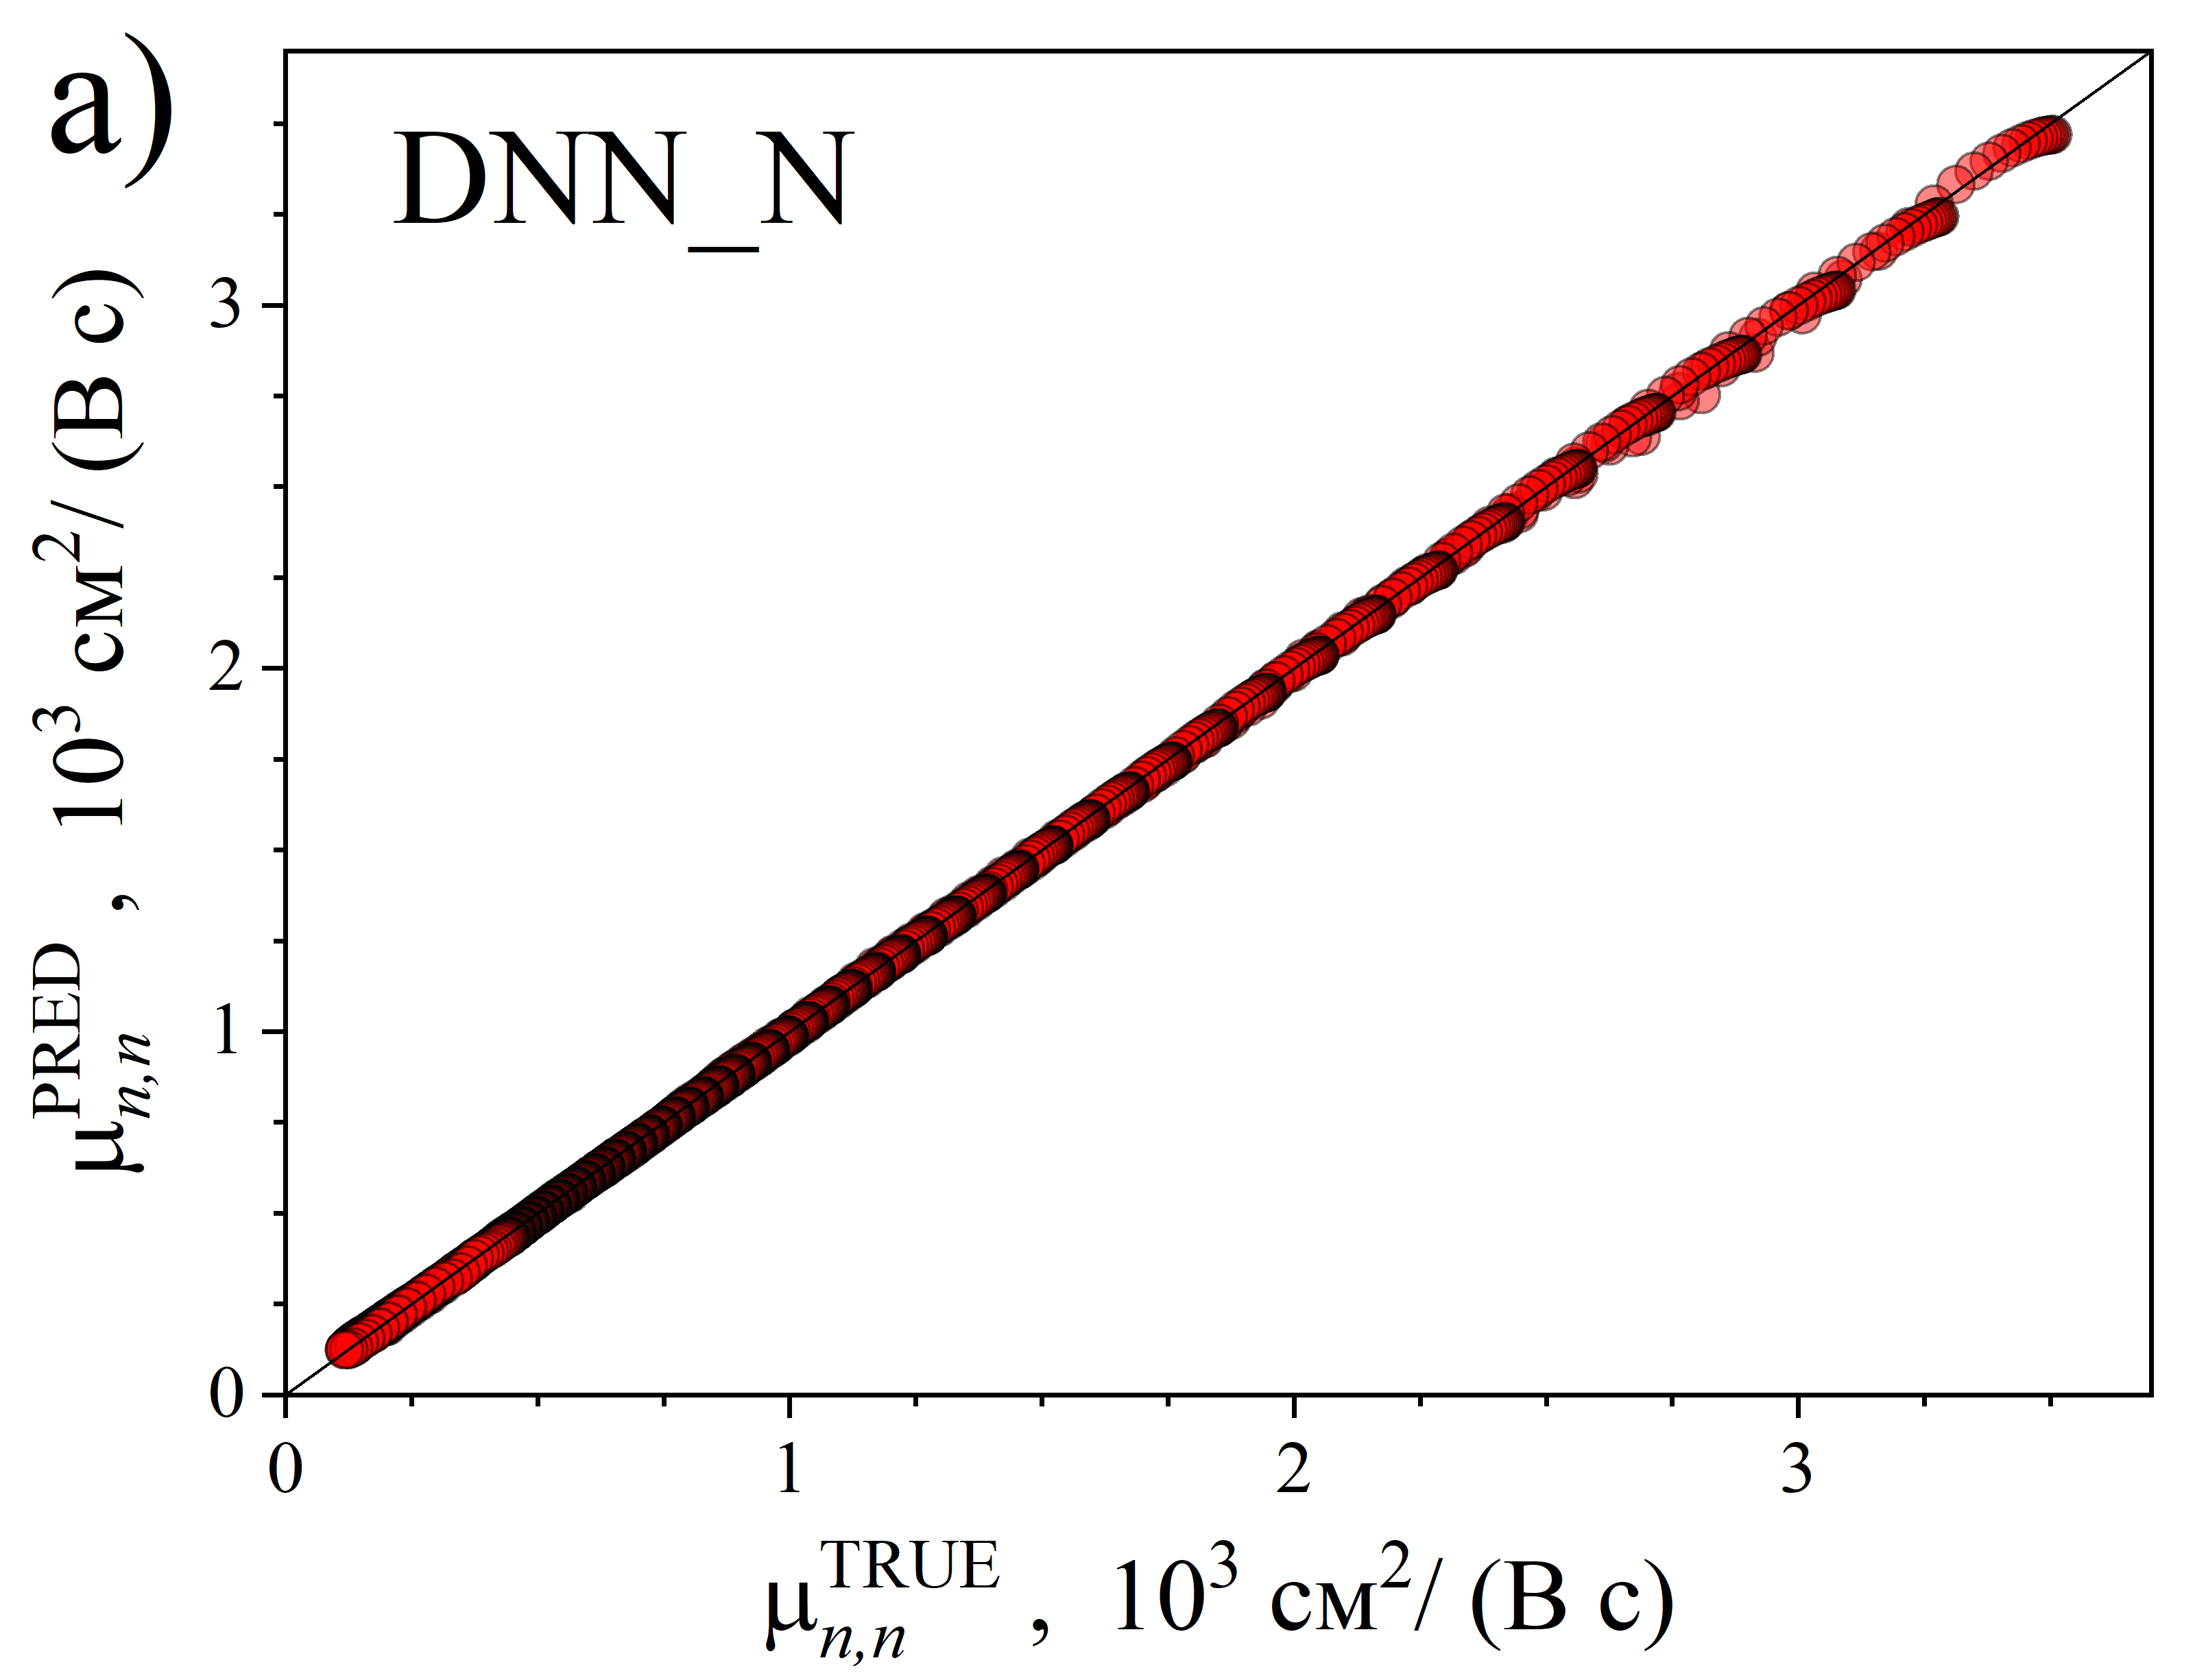
\includegraphics[width=0.35\linewidth]{DNNNnn.png}\kern 20pt
     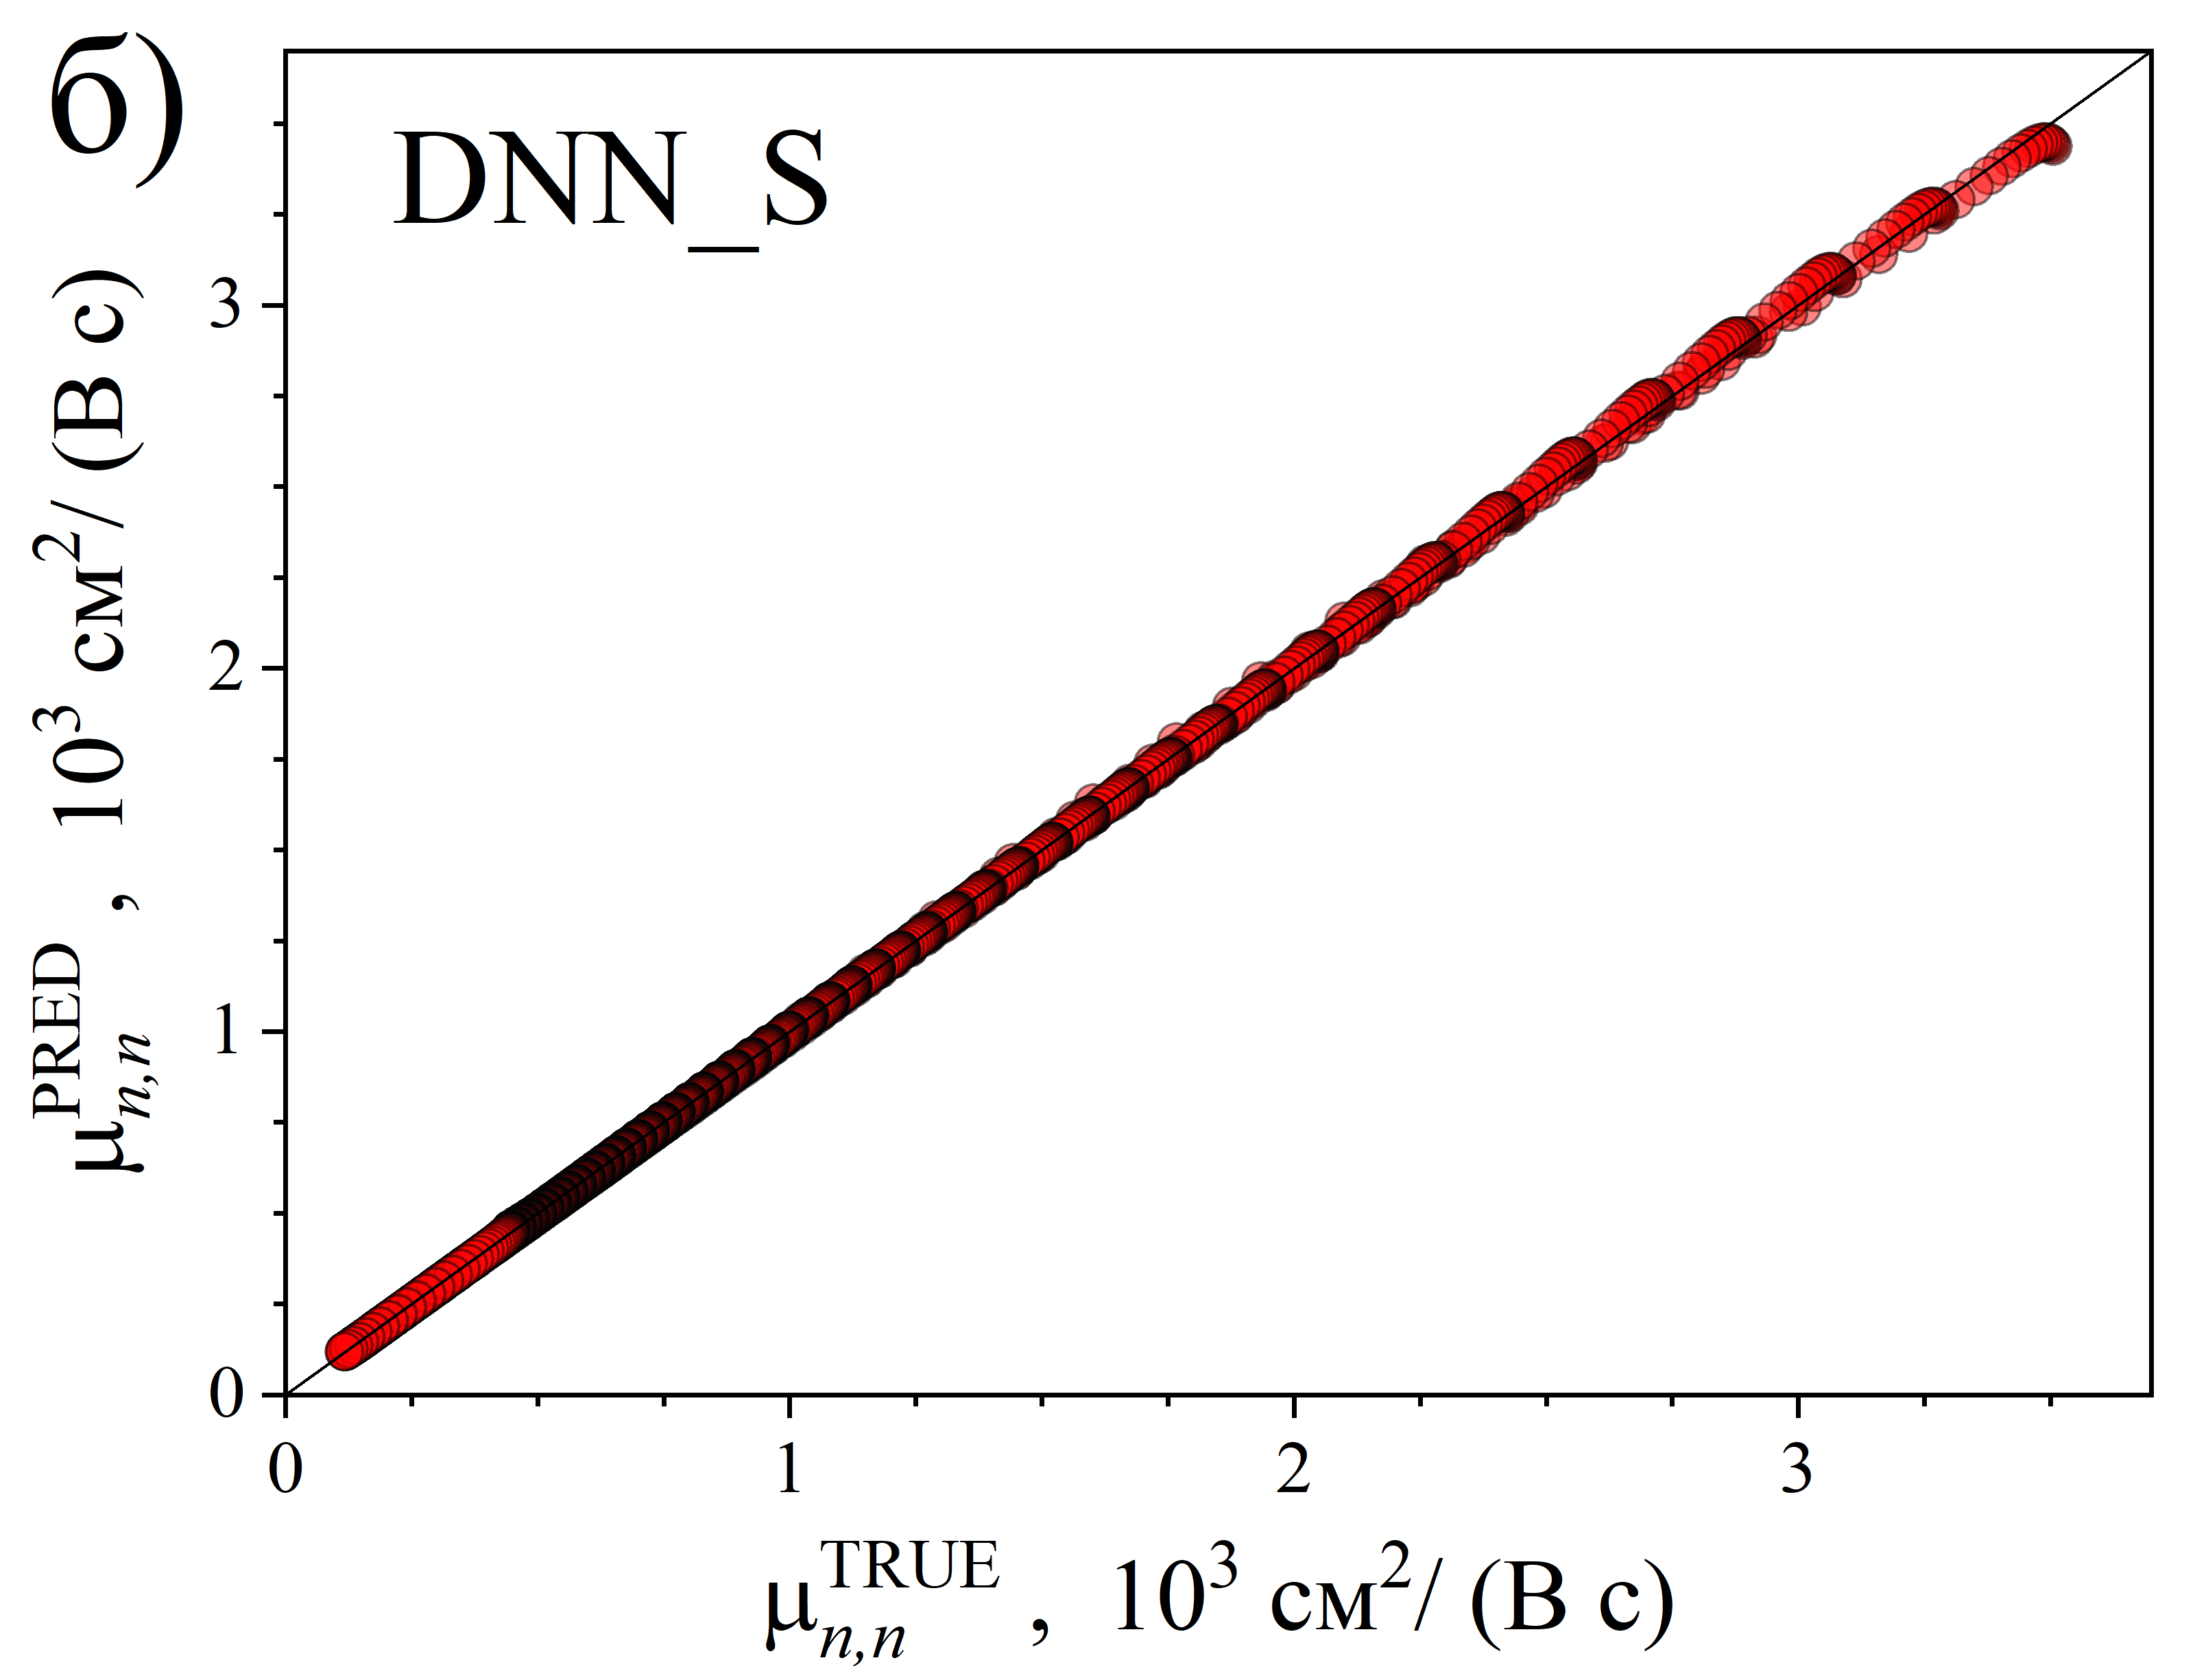
\includegraphics[width=0.35\linewidth]{DNNSnn.png}
     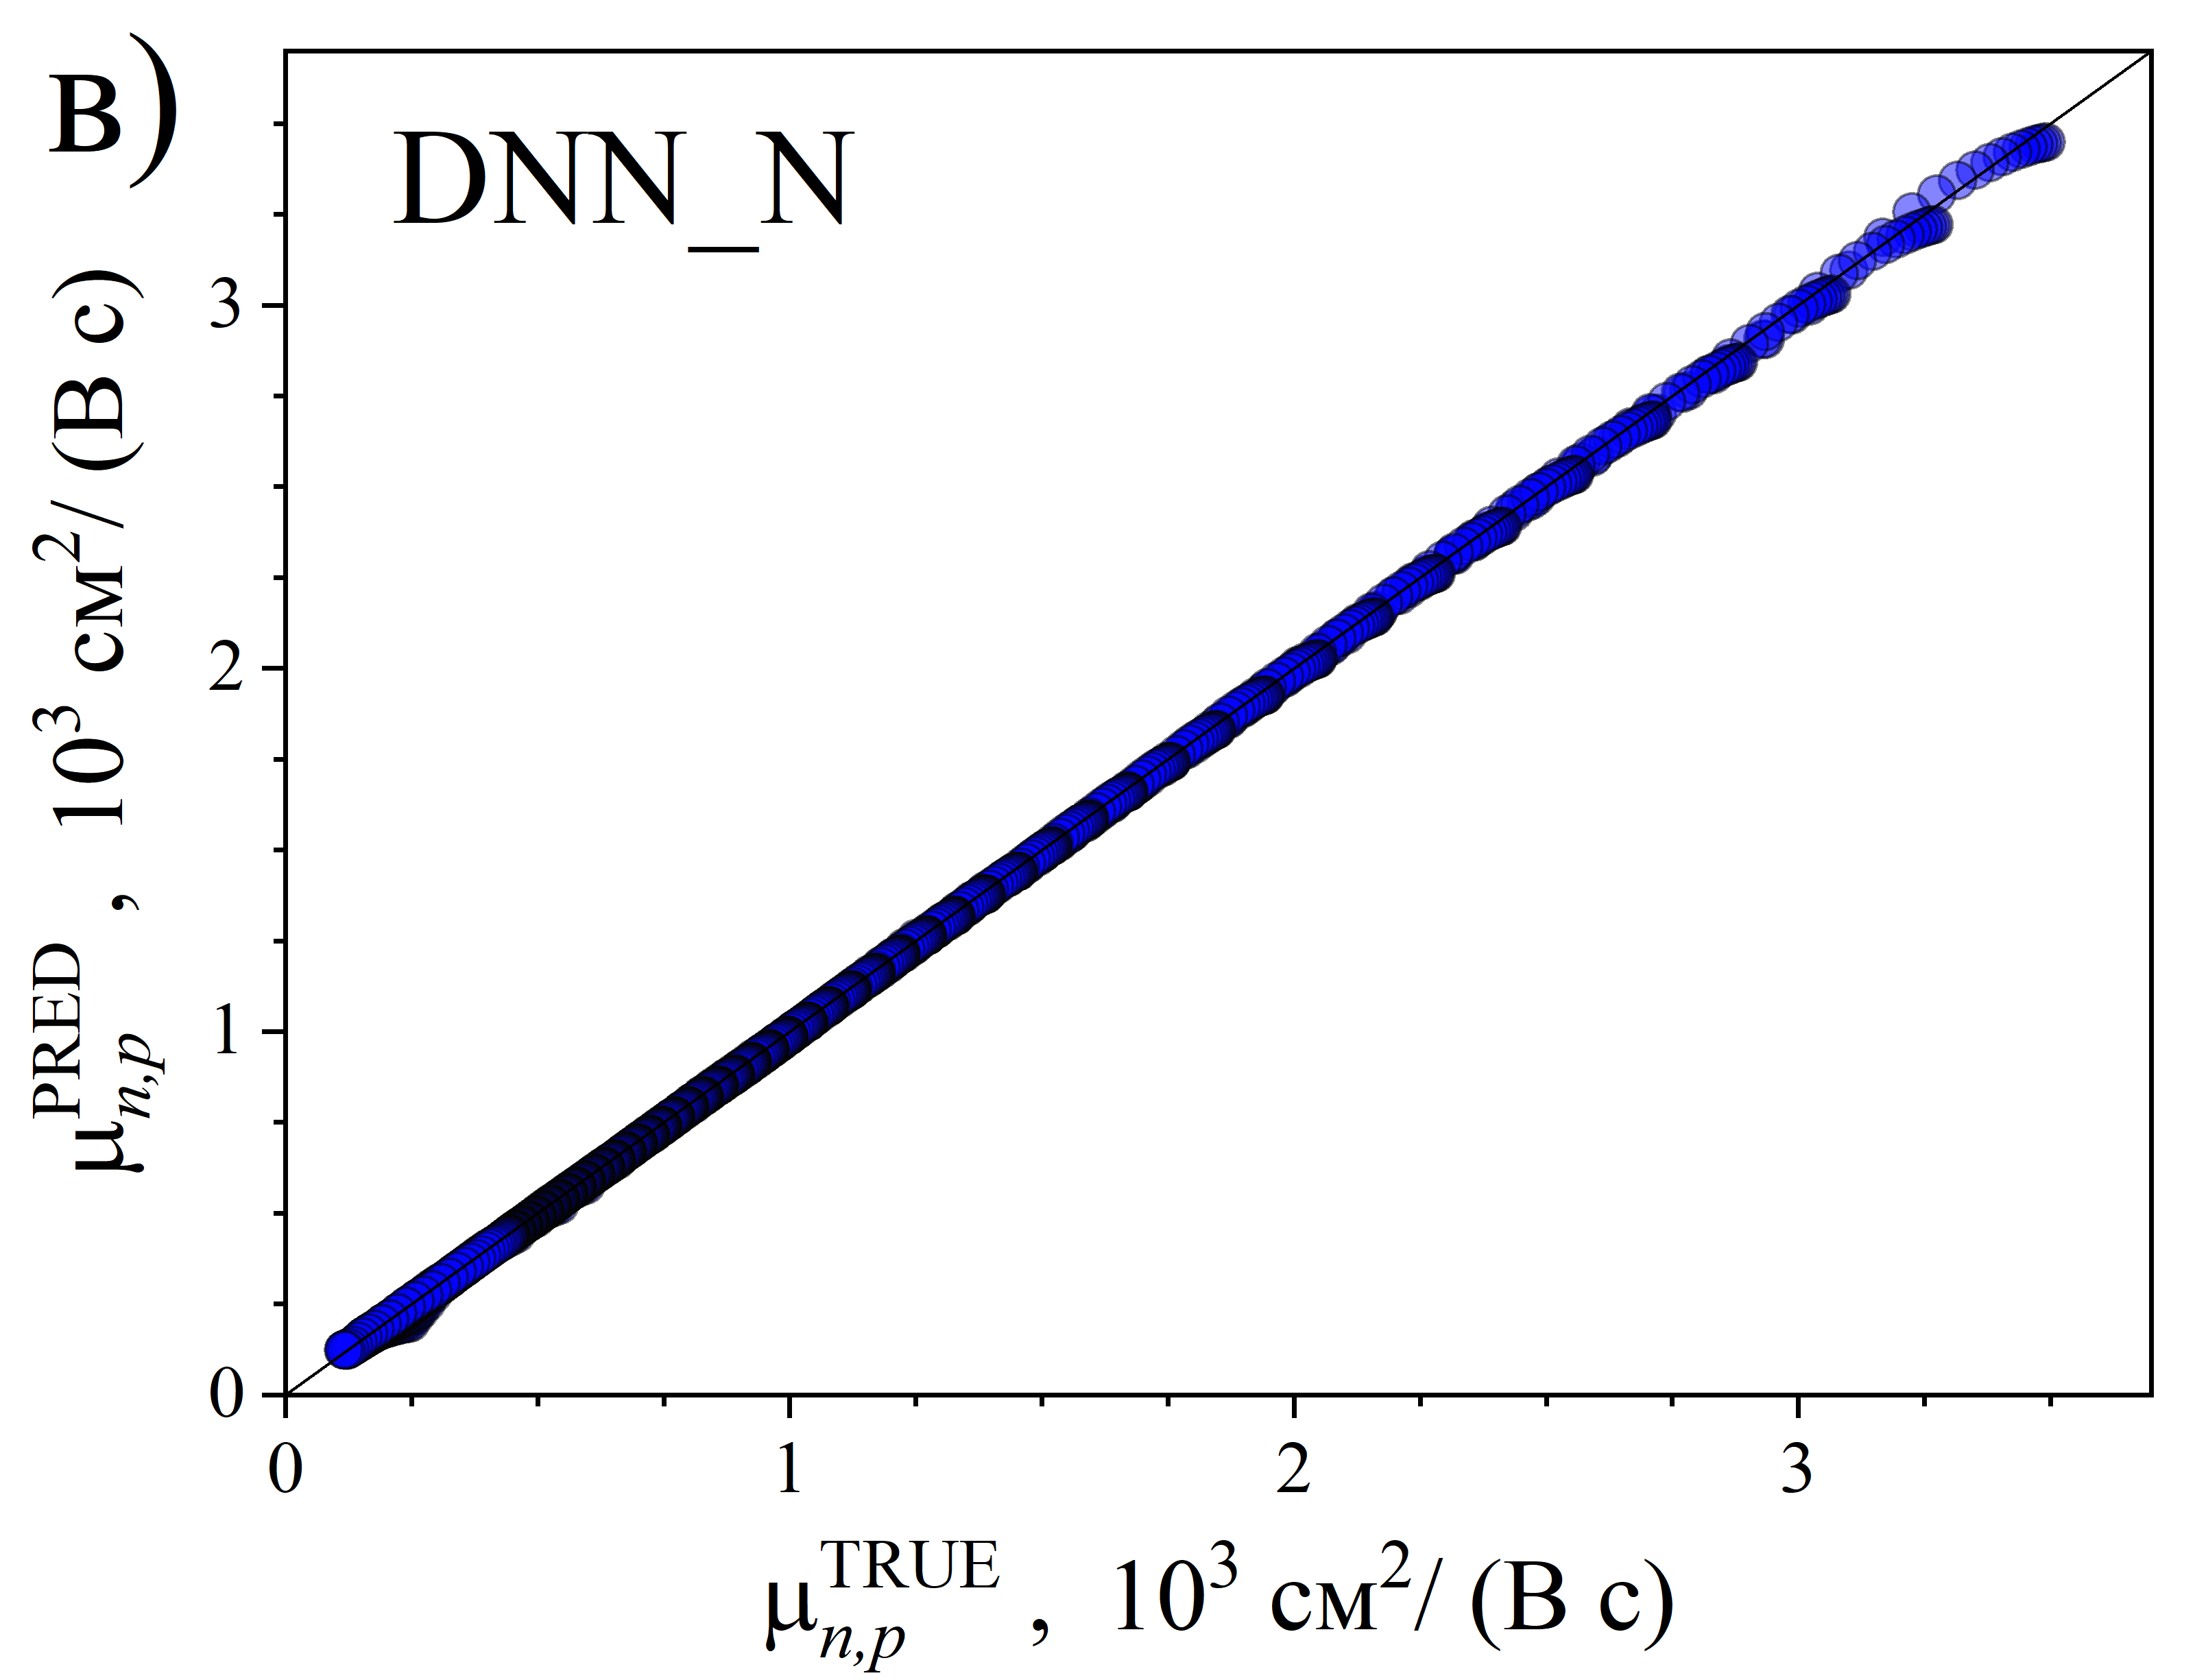
\includegraphics[width=0.35\linewidth]{DNNNnp.png}\kern 20pt
     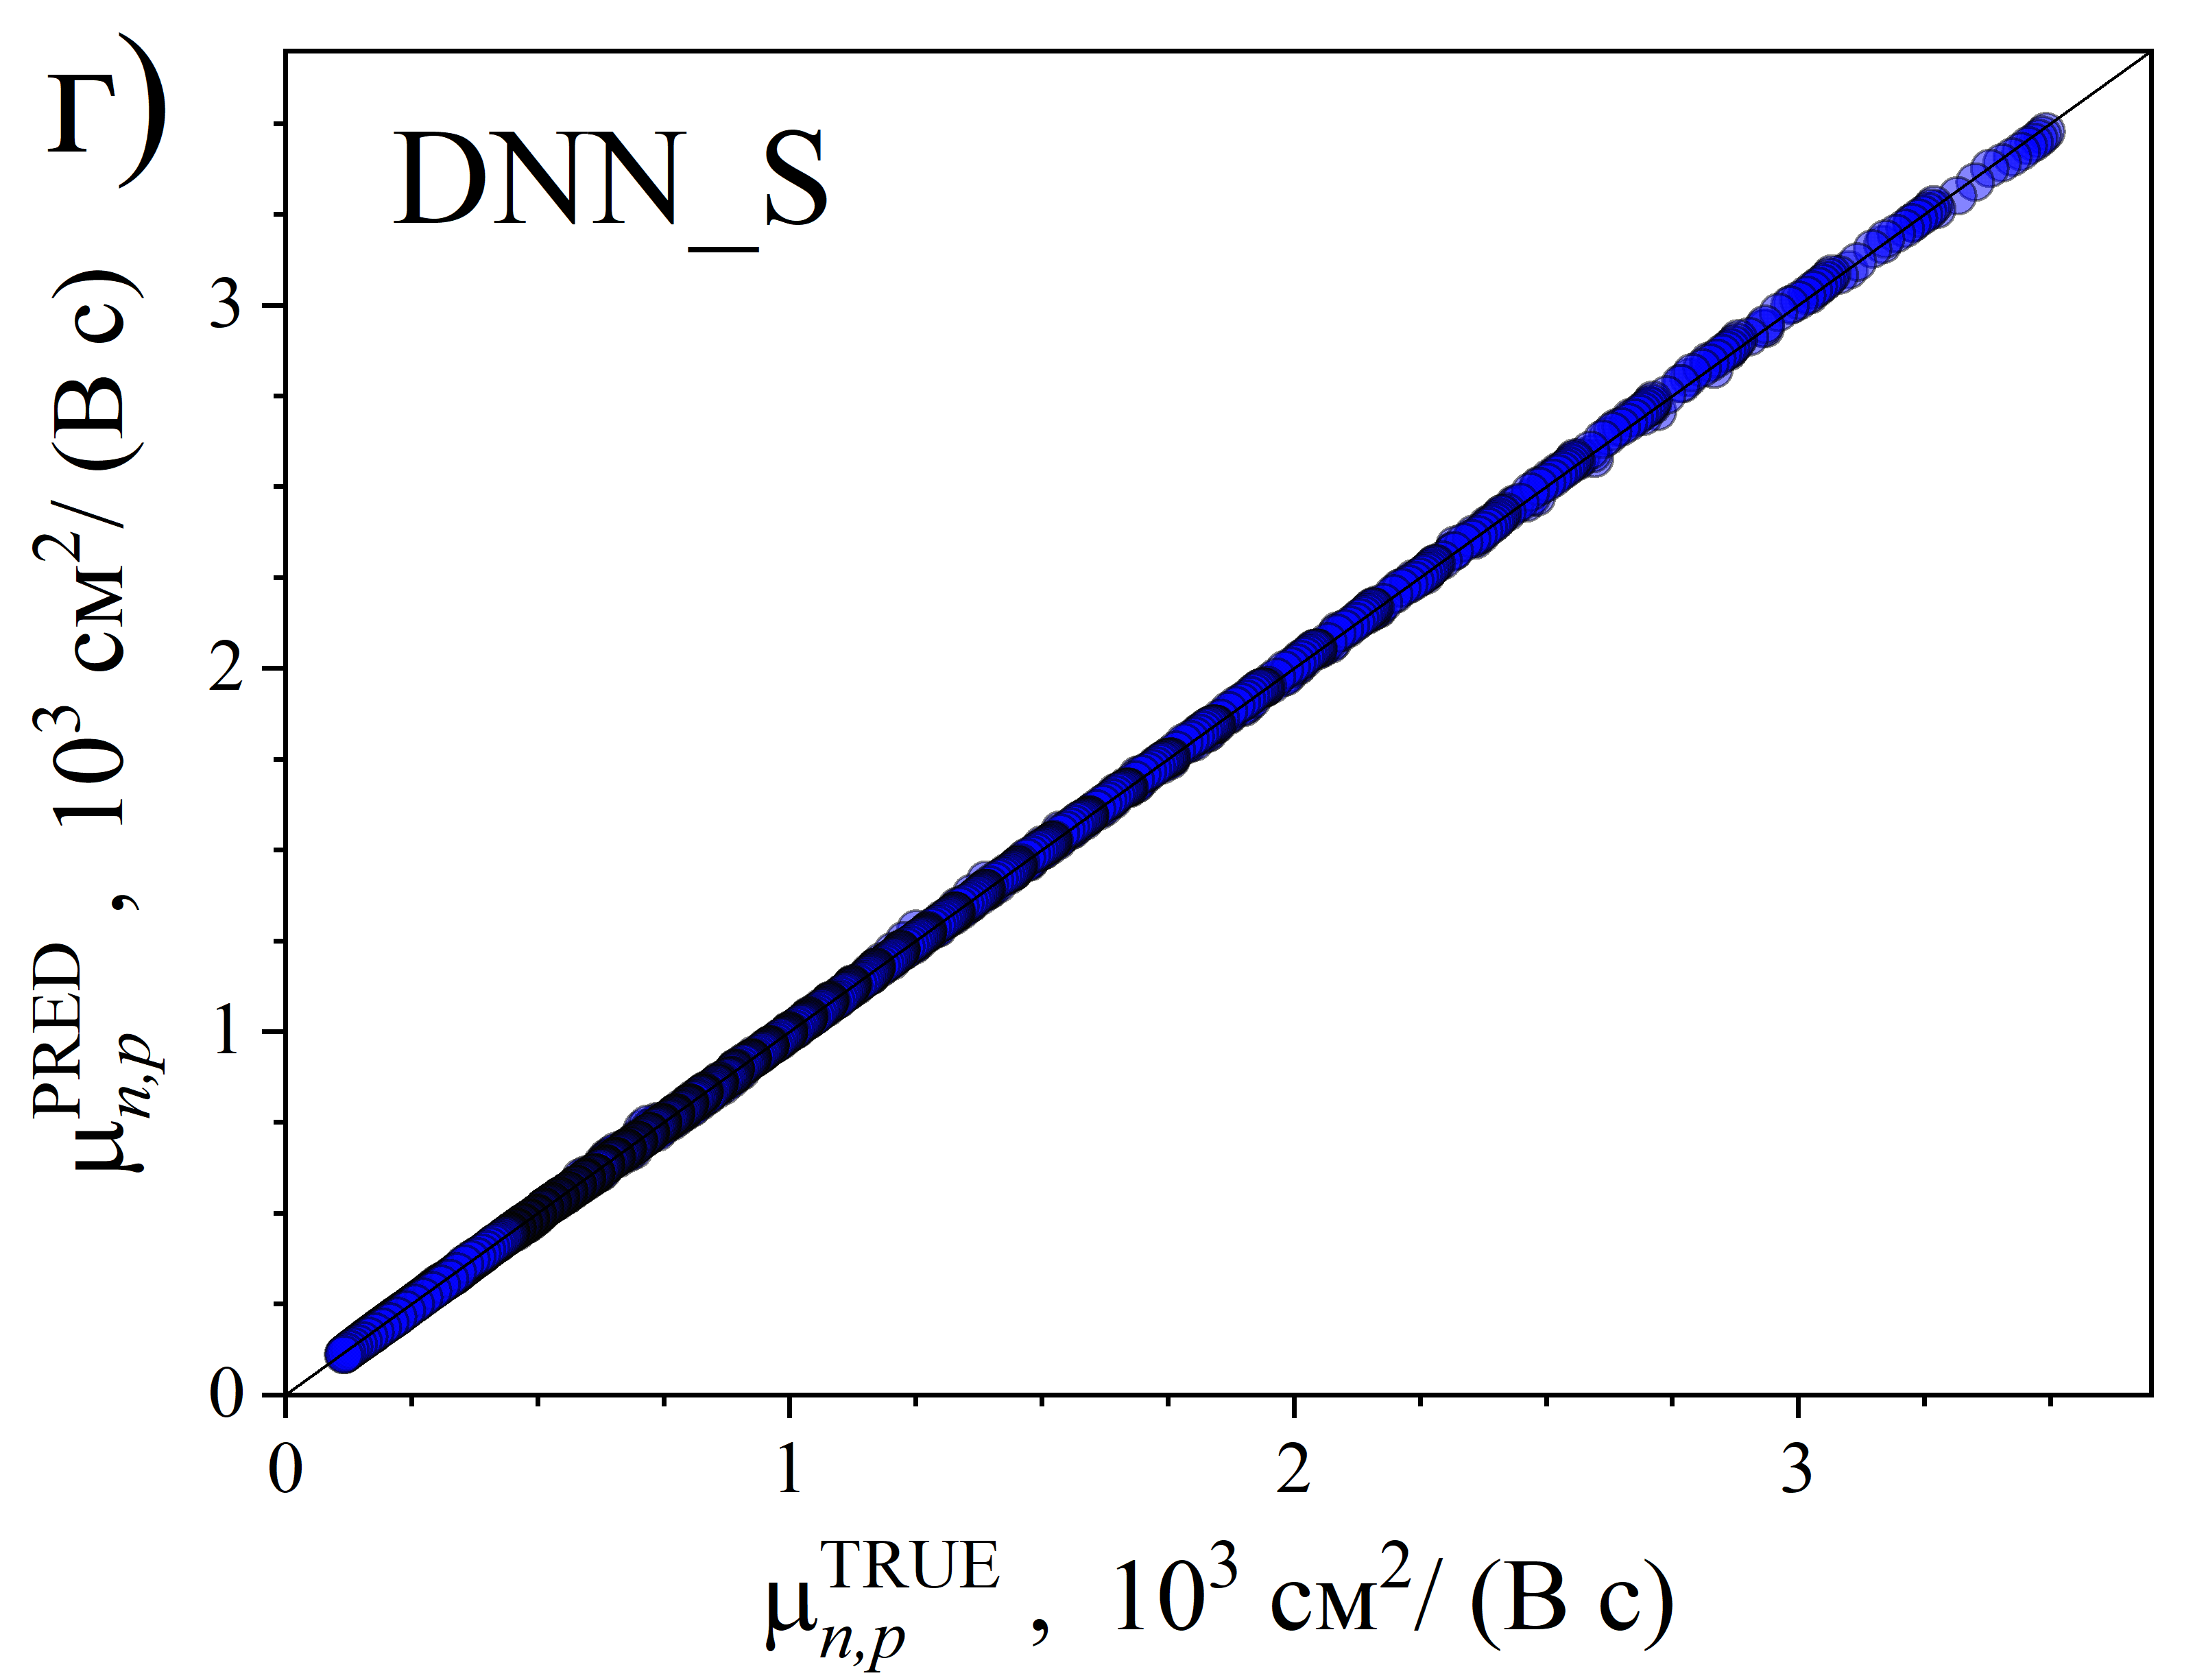
\includegraphics[width=0.35\linewidth]{DNNSnp.png}
     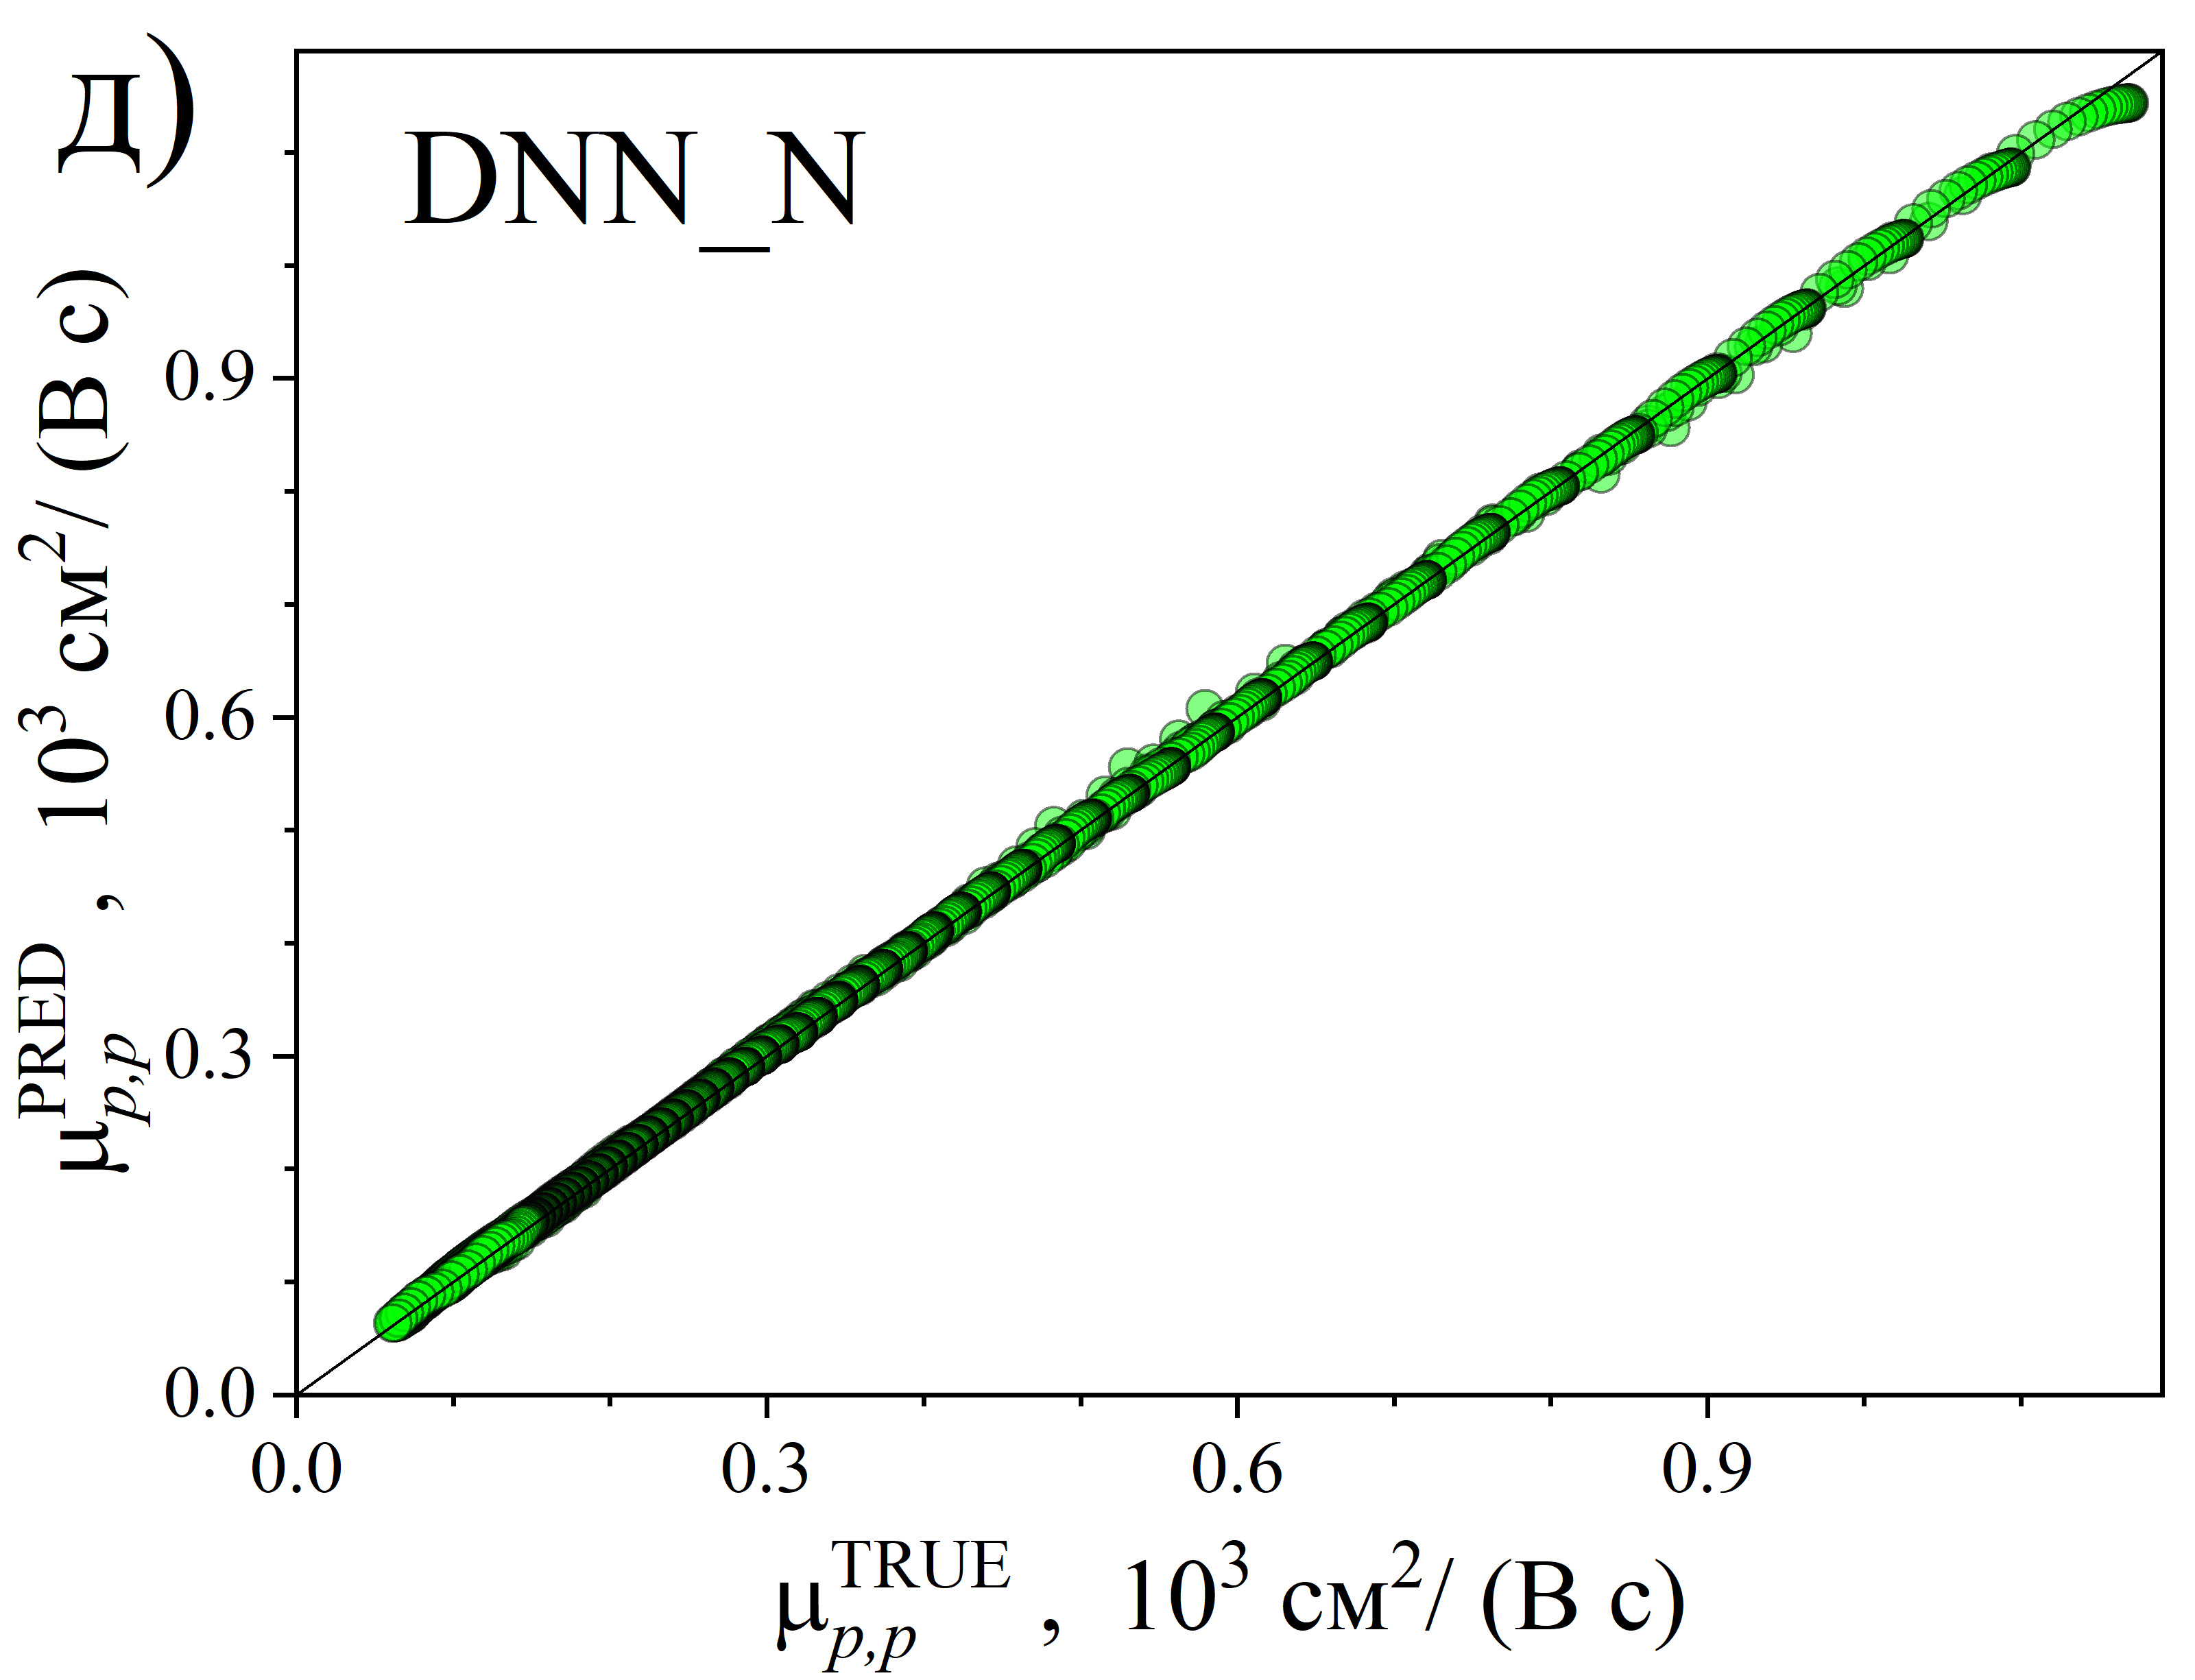
\includegraphics[width=0.35\linewidth]{DNNNpp.png}\kern 20pt
     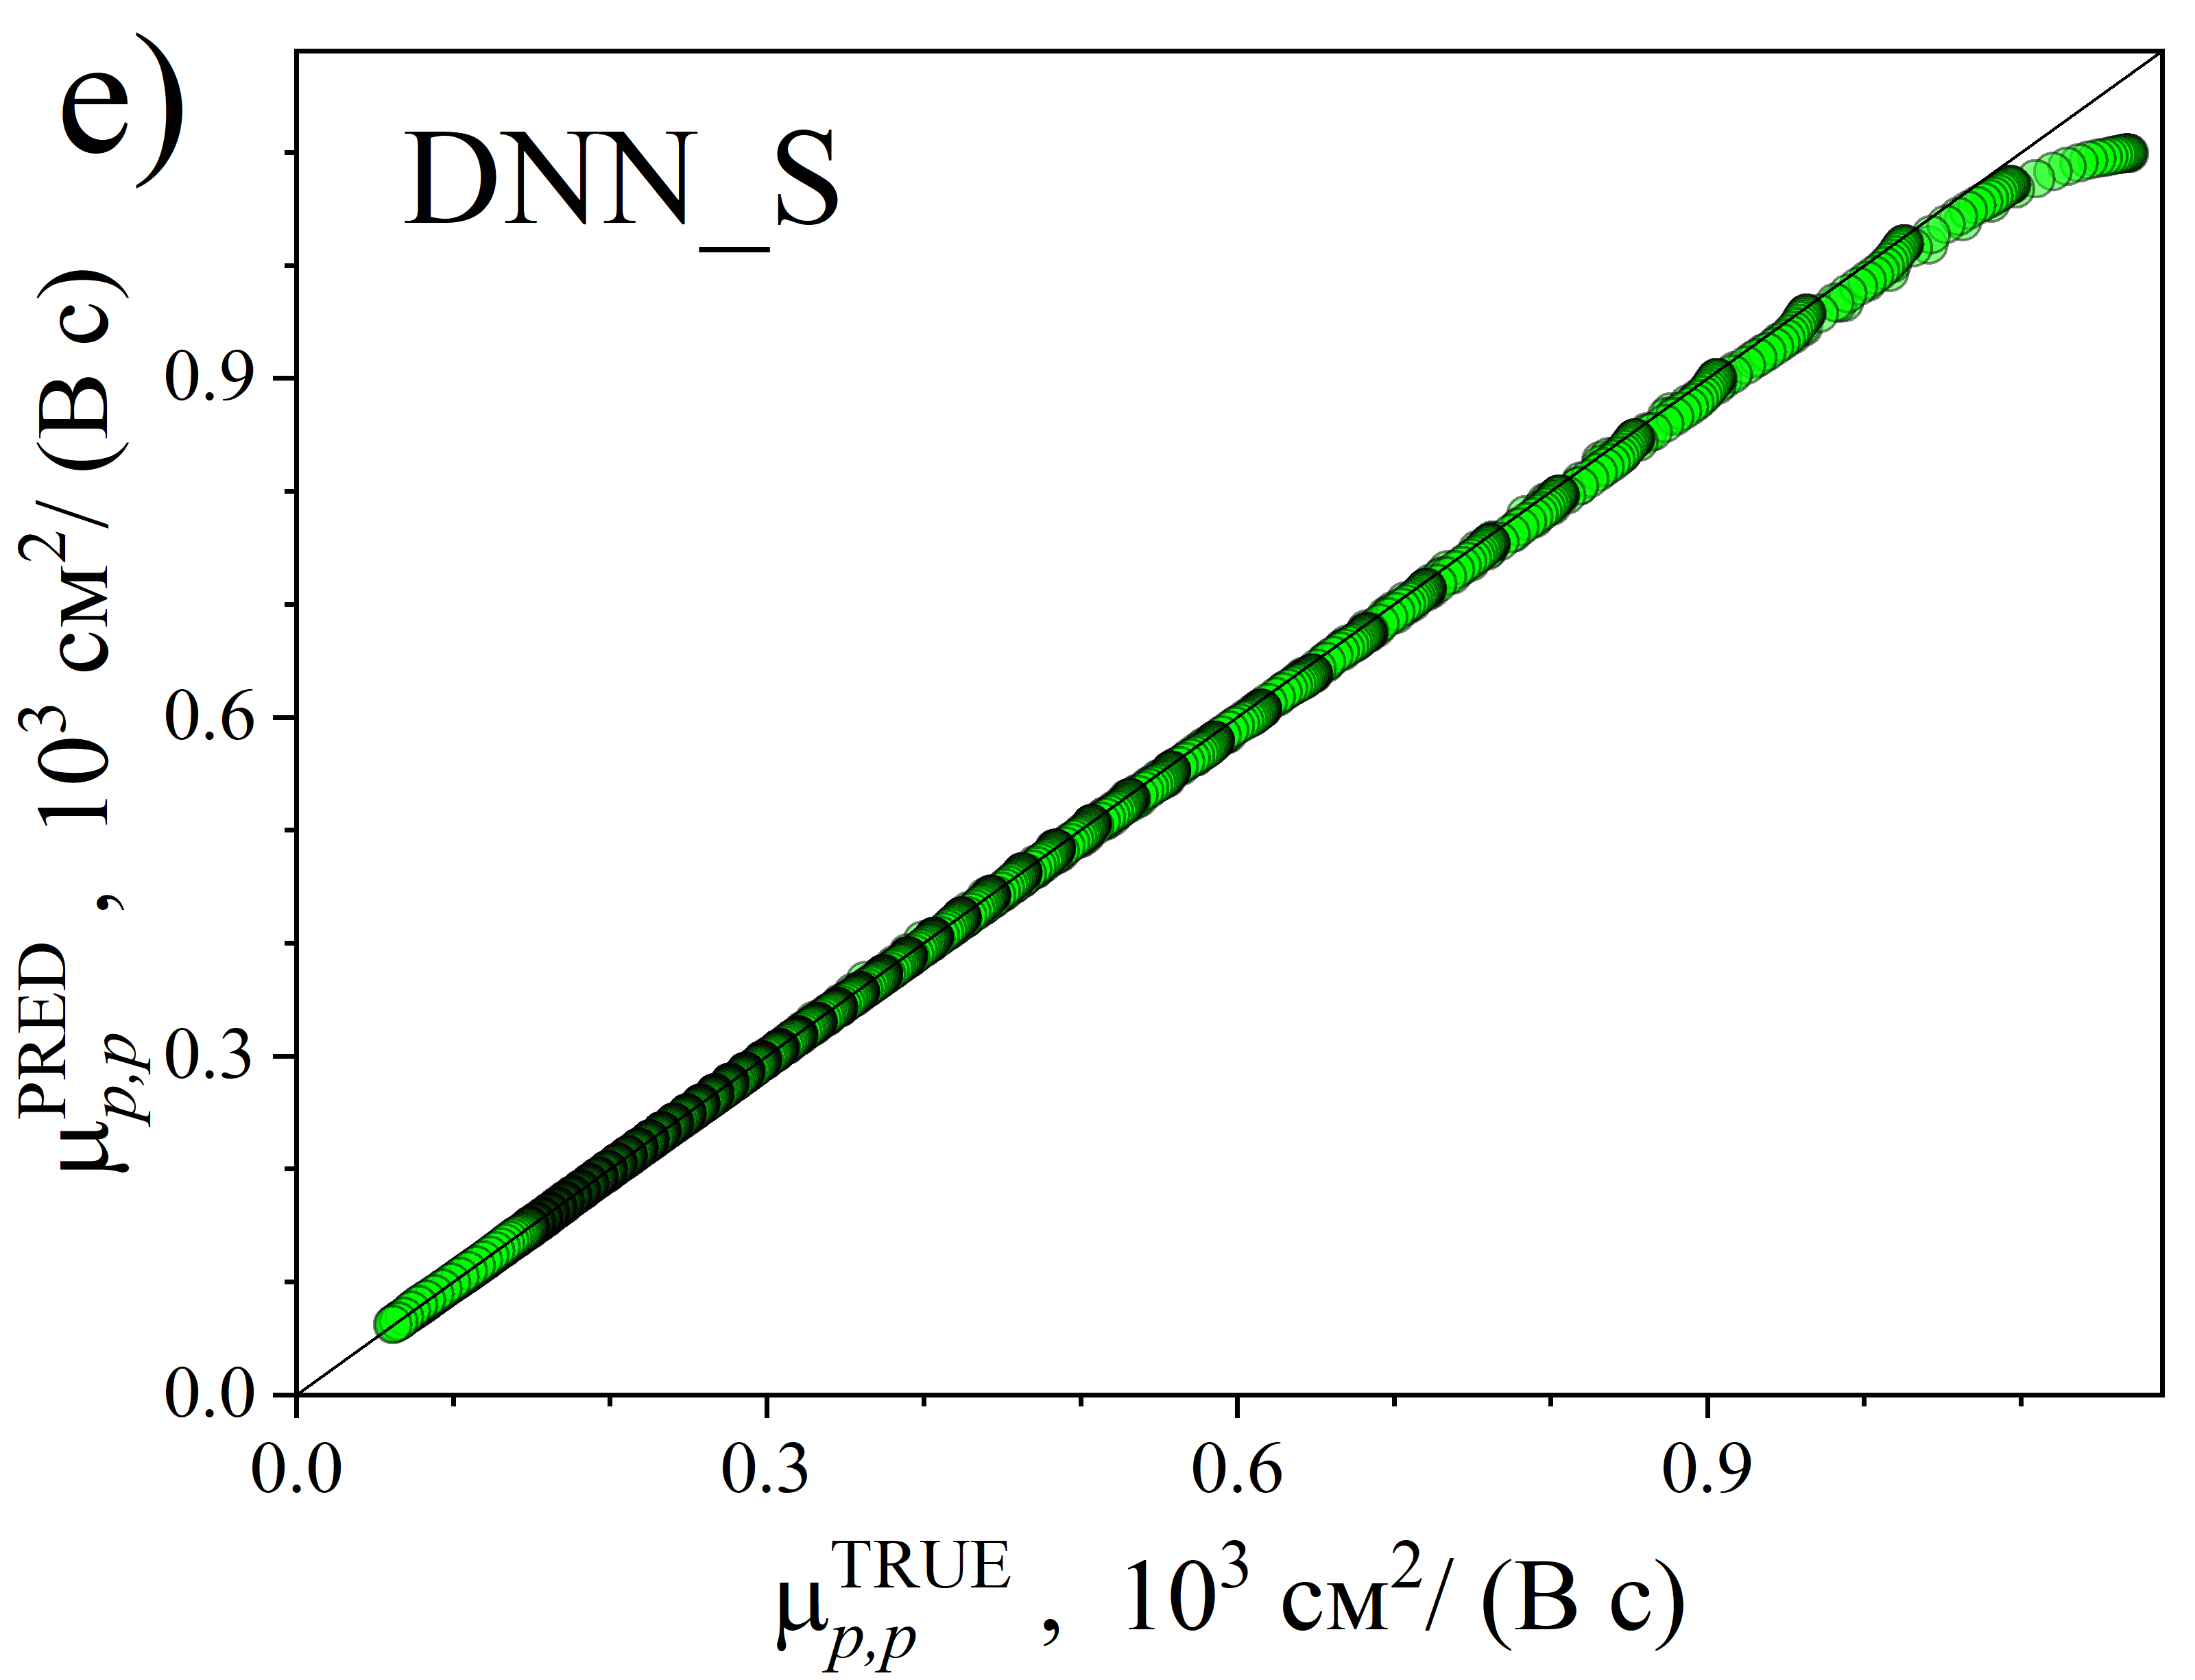
\includegraphics[width=0.35\linewidth]{DNNSpp.png}
     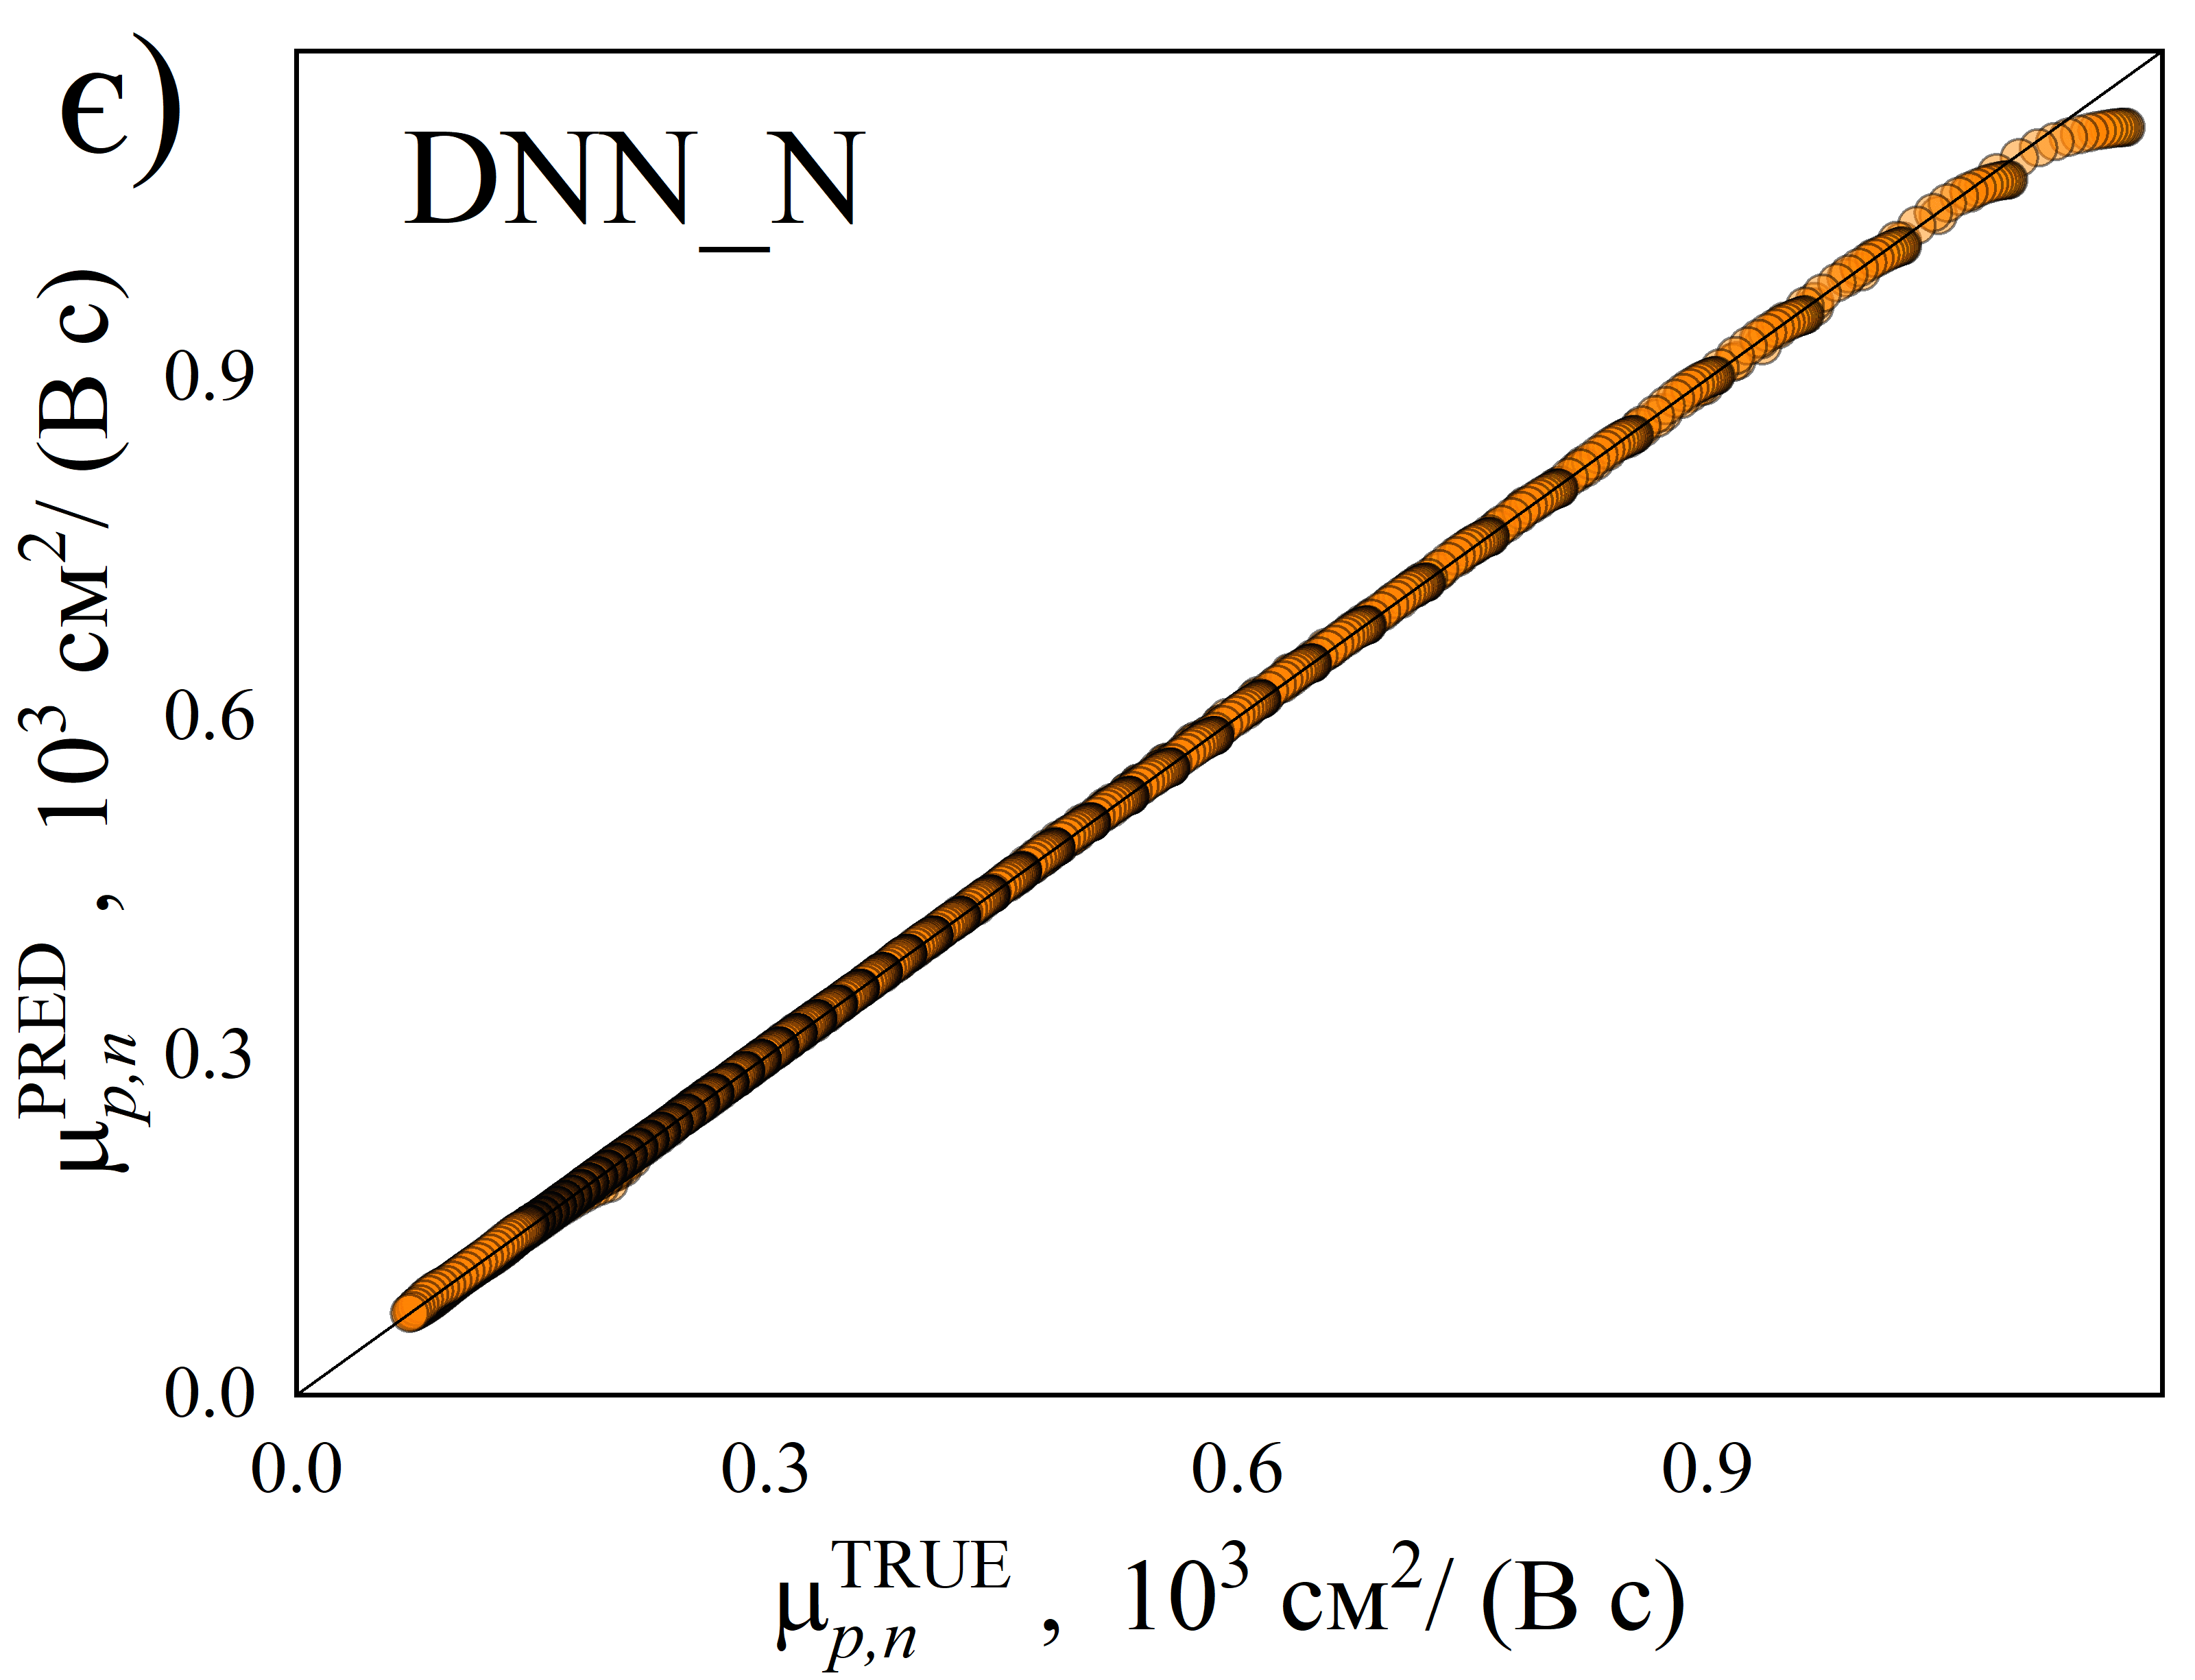
\includegraphics[width=0.35\linewidth]{DNNNpn.png}\kern 20pt
     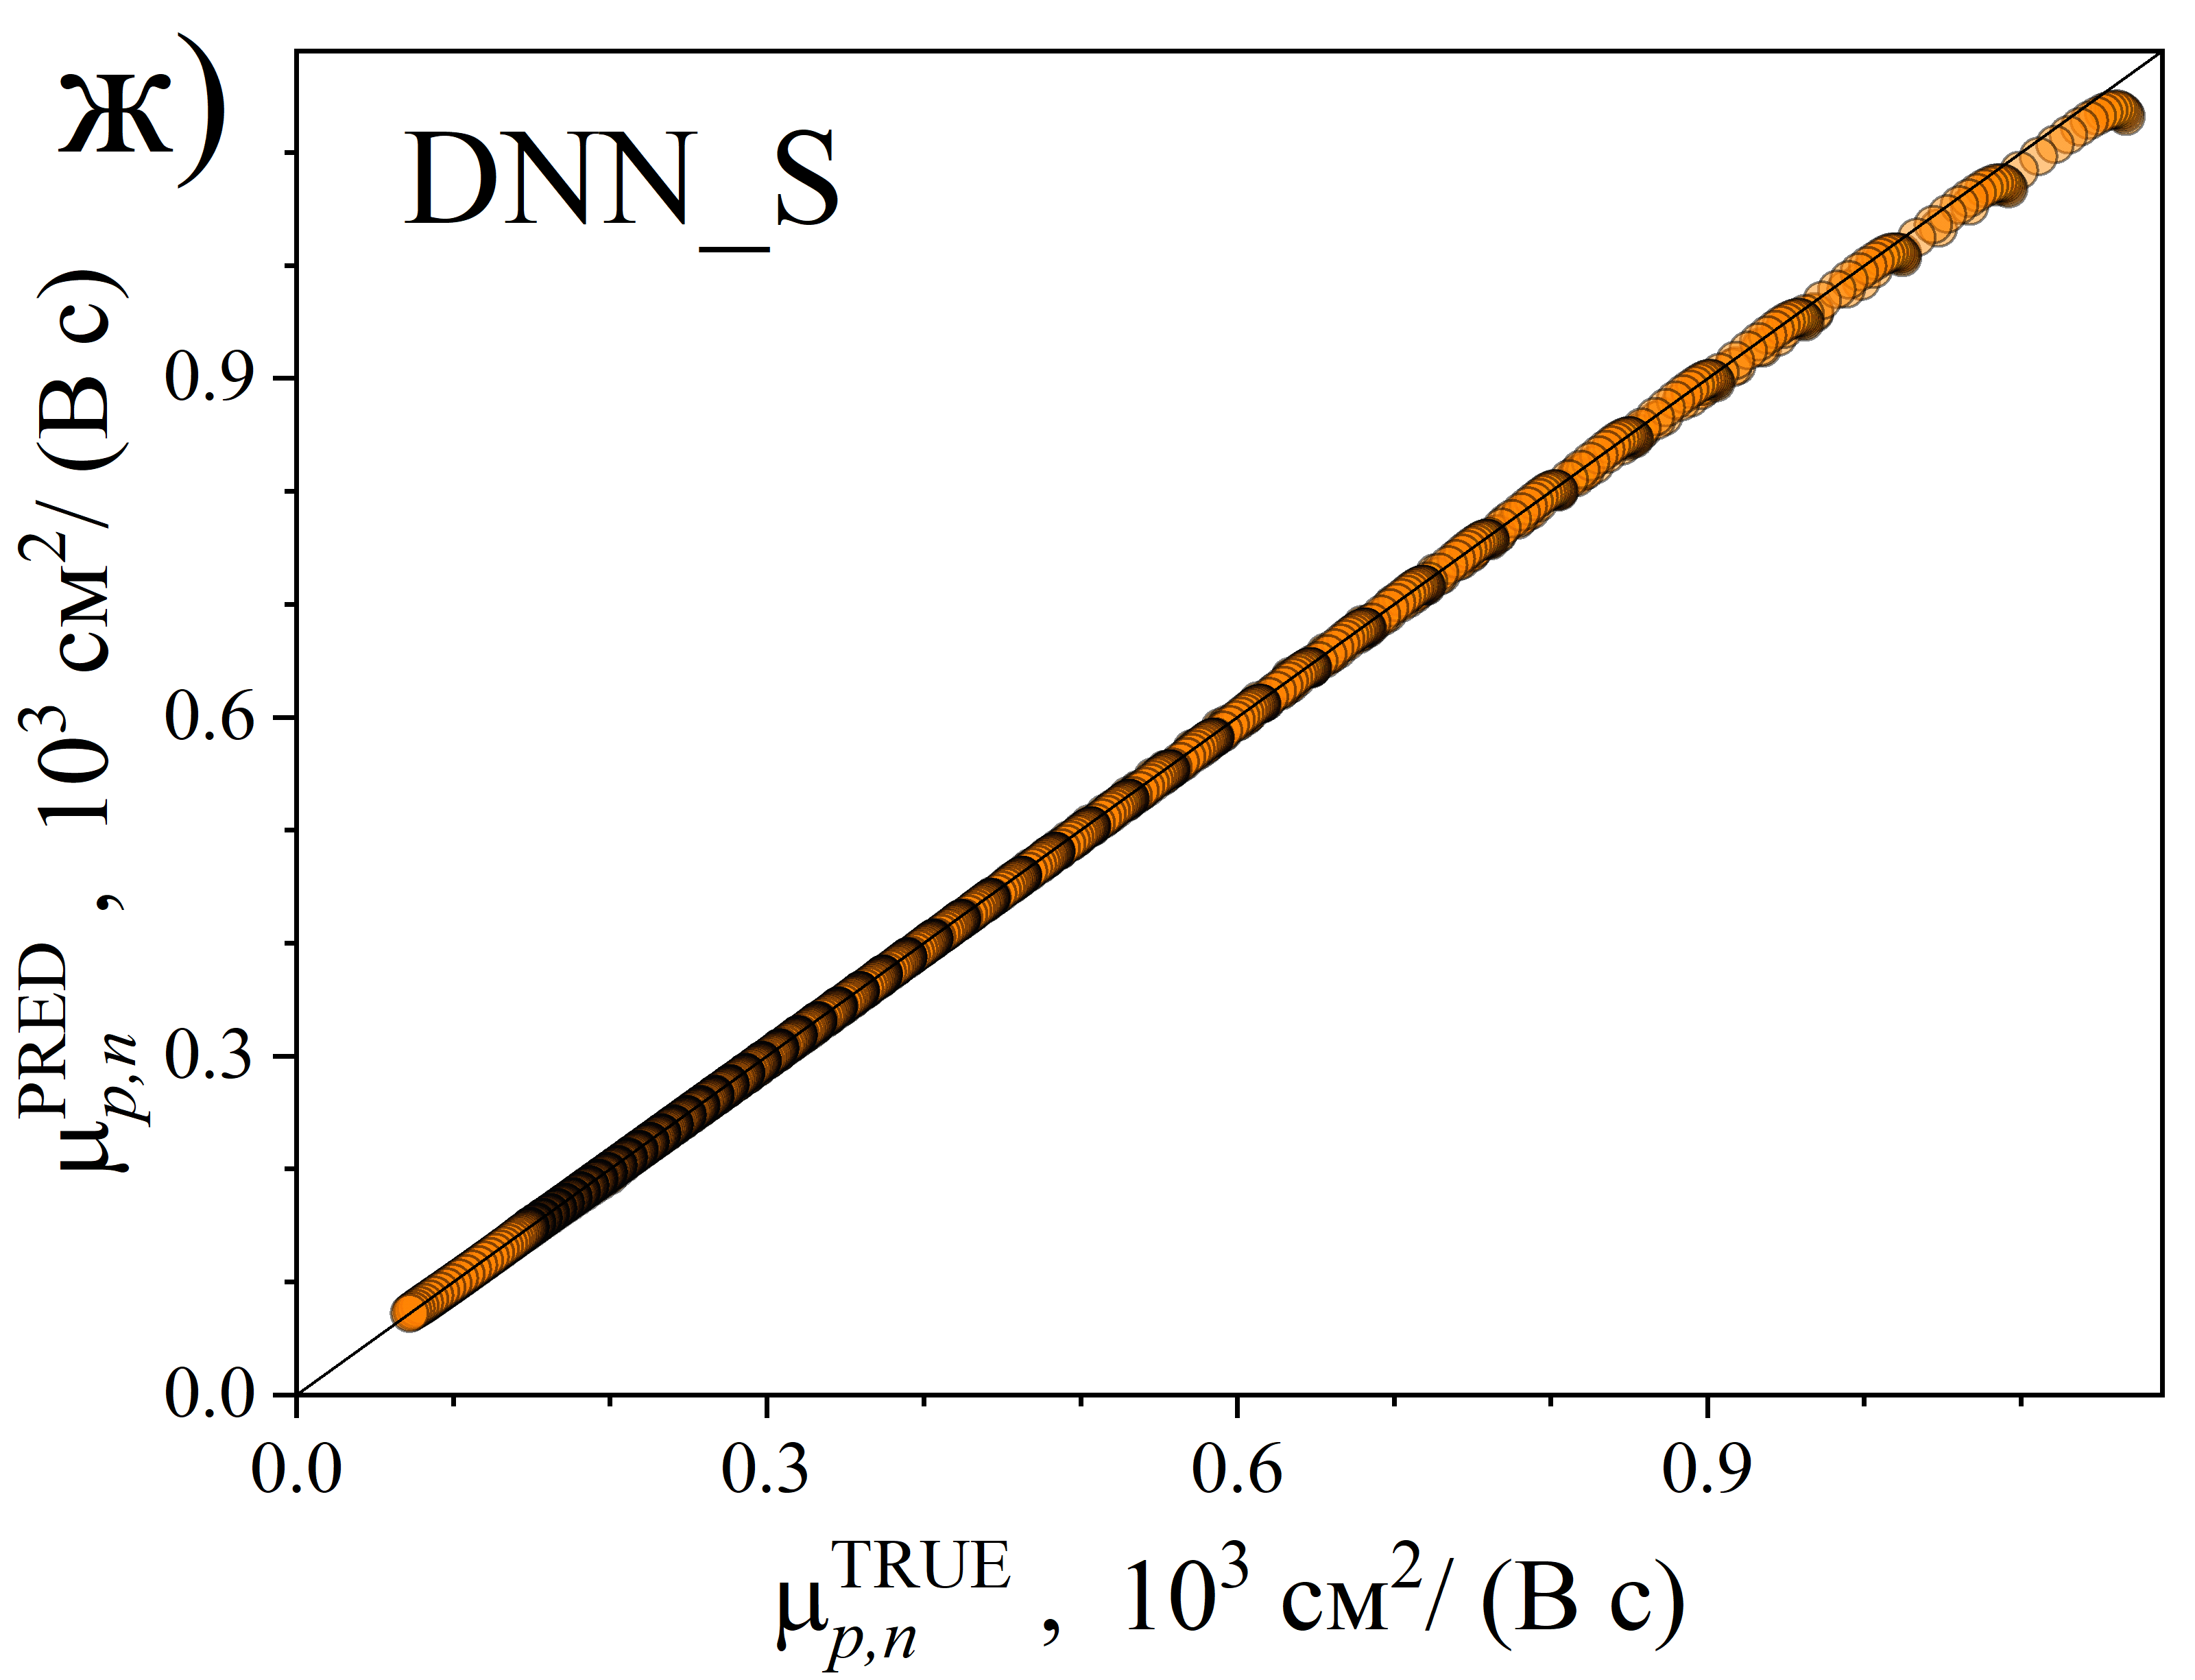
\includegraphics[width=0.35\linewidth]{DNNSpn.png}
	  \caption{Діаграми розсіювання, що порівнюють еталонні значення рухливості із значеннями, передбаченими DNN моделями 
       на тестовому наборі даних.
       Представлені випадки оцінки рухливості електронів (а--г) та дірок (д--ж), коли вони є
       основними (а, б, д, е) та неосновними (в, г, є, ж) носіями заряду.
       Попередня підготовка даних передбачала нормування (а, в, д, є) або нормалізацію (б, г, е, ж).
}\label{figDNN}
\end{figure}



\section{Порівняння точності різних алгоритмів машинного навчання}


Текст перед таблицею...

\begin{landscape}

\vspace{30mm}

\begin{table}[htbp]
%\setlength{\tabcolsep}{3pt}
\renewcommand{\arraystretch}{1.5}
\centering
\caption{Метрики відхилень розрахованих значень рухливості у кремнії від теорії Klaassen.
Жирним виділено найкращі результати для кожної метрики при передбаченнях рухливості електронів та дірок, коли вони є основними та неосновними носіями заряду}
\begin{tabular}{|l|c|c|c|c|c|c|c|c|c|c|c|c|c|c|c|c|}
\hline
\multirow{2}{*}{Модель}&\multicolumn{4}{c|}{MAPE, \%}&\multicolumn{4}{c|}{$\mathrm{APE}_\mathrm{MAX}$, \%}
   &\multicolumn{4}{c|}{$\mathrm{APE}_\mathrm{MED}$, \%}&\multicolumn{4}{c|}{MAE,$\text{см}^2/(\text{B}\cdot\text{с})$}\\
\cline{2-17}
&$\mu_{n,n}$&$\mu_{n,p}$&$\mu_{p,p}$&$\mu_{p,n}$&$\mu_{n,n}$&$\mu_{n,p}$&$\mu_{p,p}$&$\mu_{p,n}$
&$\mu_{n,n}$&$\mu_{n,p}$&$\mu_{p,p}$&$\mu_{p,n}$&$\mu_{n,n}$&$\mu_{n,p}$&$\mu_{p,p}$&$\mu_{p,n}$\\
\hline
Arora \cite{Arora1982}&5,35&20,3&5,62&37,8&38,2&70,7&17,6&111&3,67&16,3&5,01&32,6&45,7&103&16,0&82,6\\
\hline
RF\_N &1,29&1,69&1,52&1,47&9,33&14,5&4,60&10,9&0,805&0,994&0,264&0,913&11,0&13,5&4,50&4,76\\
\hline
RF\_S&1,42&1,77&1,46&1,41&12,3&14,4&14,5&12,6&0,852&1,04&0,744&0,872&11,6&14,1&4,40&4,76\\
\hline
SVR\_N&46,5&51,5&32,6&33,4&1630&1750&2070&1510&14,9&17,4&13,1&12,9&220&244&68,8&73,6\\
\hline
SVR\_S&0,108&\textbf{0,087}&\textbf{0,098}&0,082&1,71&2,16&2,26&3,56&0,088&\textbf{0,064}&\textbf{0,069}&0,050&1,20&1,03&0,394&0,410\\
\hline
GB\_N&2,20&1,46&1,60&1,55&58,2&10,8&17,3&11,0&1,46&0,939&0,905&1,15&15,43&10,85&4,75&5,24\\
\hline
GB\_S&1,32&1,60&1,82&1,23&1,42&11,7&15,0&8,48&0,841&1,104&1,19&0,874&11,3&13,4&5,92&4,19\\
\hline
DNN\_N&0,925&0,942&2,01&0,529&9,39&20,0&8,07&6,02&0,621&0,702&1,893&0,383&5,23&5,37&4,22&1,39\\
\hline
DNN\_S&0,374&0,623&0,655&0,671&2,23&3,75&5,96&2,97&0,323&0,392&0,556&0,631&3,58&3,49&2,88&1,97\\
\hline
SR&\textbf{0,094}&0,137&0,140&\textbf{0,050}&\textbf{1,19}&\textbf{0,992}&\textbf{1,48}&\textbf{0,596}&\textbf{0,044}&0,077&0,079&\textbf{0,026}&\textbf{0,475}
   &\textbf{0,708}&\textbf{0,314}&\textbf{0,115}\\
\hline
\end{tabular}
\end{table}
\end{landscape}

Текст після таблиці...




\chapter*{Висновки}



%Carrier mobility in a semiconductor is one of the most
%important parameters for the operation of electronic
%devices. Actually, the mobility measures the ability of
%free carriers (electrons or holes) to move in the material
%as it is subjected to an external electric field. The magni-
%tude of the mobility directly impacts on the device perform-
%ance since it determines the operation speed through the
%transit time across the device, the circuit operating fre-
%quency, or the sensitivity in magnetic sensors.

%THE ELECTRON tion of dopant concentration and temperature and hole mobilities in silicon as a func- are
%important parameters for device design and analysis.


%\begin{titlepage}
\begin{center}

{\small Київський національний університет  імені Тараса Шевченка}

{\small фізичний факультет}


\vspace*{2cm}
{\scshape\bfseries\Large О.Я.~ОЛІХ}

\vspace*{1cm}
{\scshape\bfseries\huge методи дослідження дефектів}

\vspace*{0.5cm}
методичний посібник для студентів фізичного факультету

\end{center}
%
%%\vspace*{1cm}
\begin{figure}[h]\center
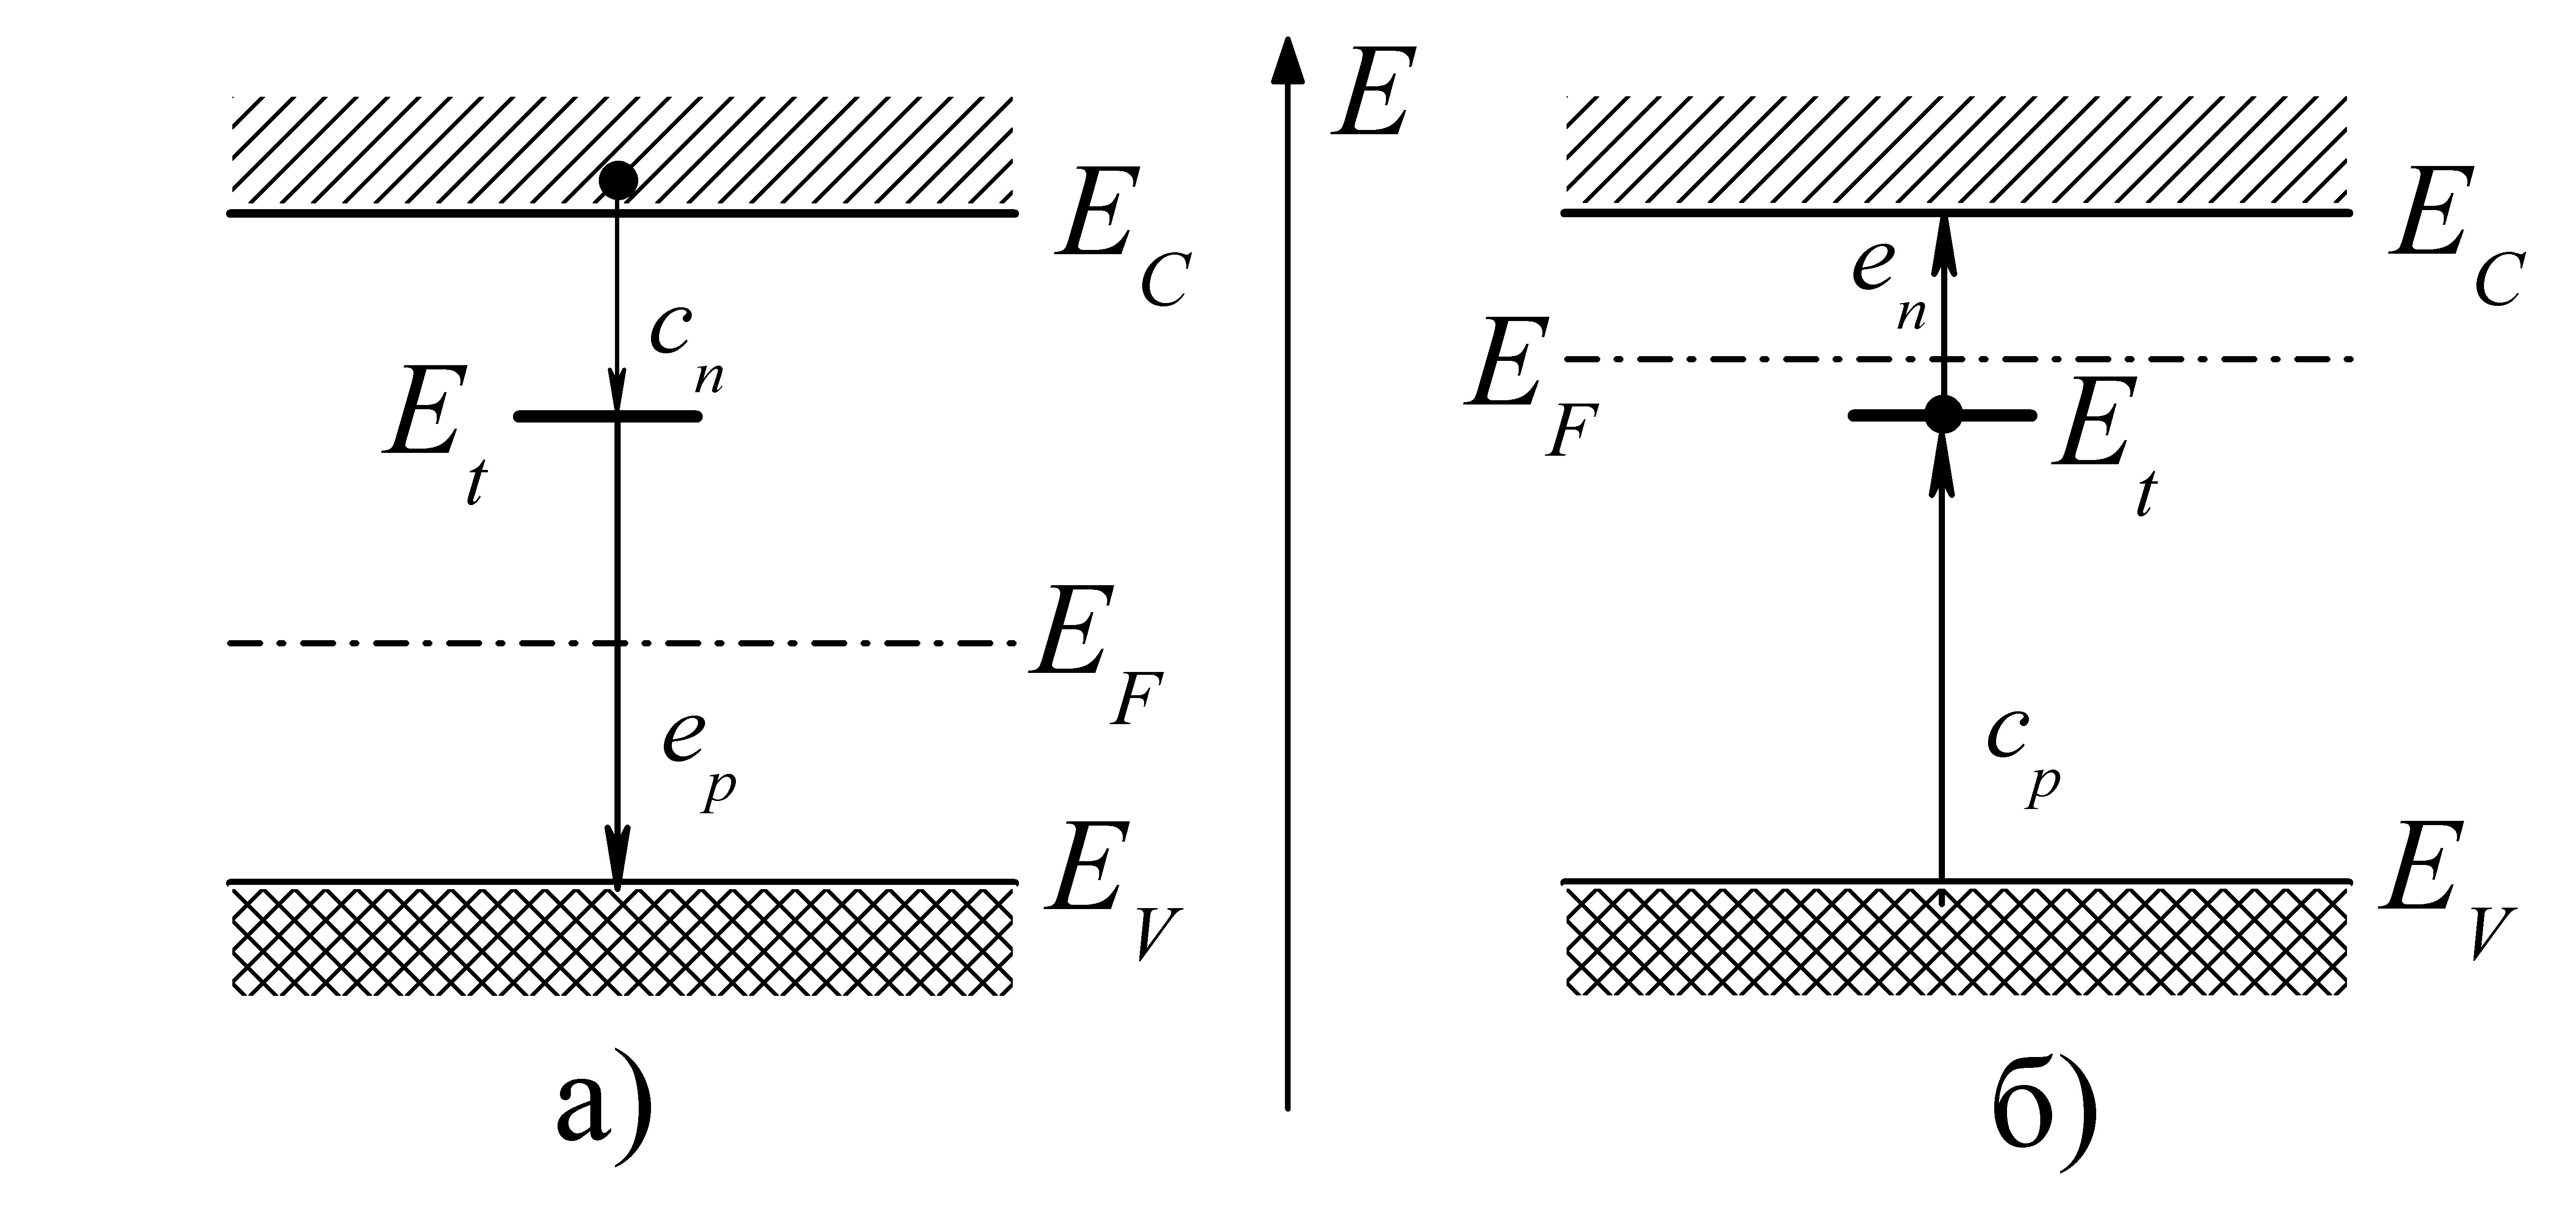
\includegraphics[width=0.4\textwidth]{Fig1_1}
\end{figure}
%
%
\begin{center}

{\scshape\bfseries Київ -- 2020}
\end{center}
\end{titlepage}
Б

УДК 004.7; 004.057.4.

\begin{center}

 \vspace{0.04\textheight}
 Рецензенти:
\end{center}
%\vspace{0.5cm}

\emph{С.В.~Кондратенко}, д-р. фіз.-мат. н., проф.

\emph{О.О.~Коротченков}, д-р. фіз.-мат. н., проф.

\vspace{1cm}
Рекомендовано до друку вченою радою фізичного факультету
Київського національного університету імені Тараса Шевченка
(протокол №10 від 18 квітня 2020 року)



\vspace{1cm}
\textbf{Оліх О.Я.}

Методи дослідження дефектів. Методичний посібник для студентів фізичного факультету. --- К.:2020.
%Іл.~236, табл.~51.

\vspace{1cm}
У посібнику розглянуто основні типи точкових дефектів, методи їх опису та термодинамічні підходи оцінки рівноважної концентрації.
Докладно викладено питання, які стосуються механізмів дифузії точкових дефектів.
Проаналізовано шляхи впливу на дефектну підсистему кристалів радіаційного опромінення і термічної обробки.
Наведено приклади найпоширеніших точкових комплексів у кремнії, а також розглянуто особливості метастабільних та бістабільних дефектів і центрів з від’ємною кореляційною енергією. Посібник містить задачі для самостійного розв’язання. 


%\renewcommand{\theequation}{\thepart.\arabic{equation}}
%\renewcommand\bibname{Рекомендована та використана література}

%\renewcommand{\thesection}{\arabic{chapter}.\arabic{section}.}
\vspace{-5cm}
\setcounter{page}{3}

%\clearpage
%%{\footnotesize
% \tableofcontents
% %}

%\renewcommand{\thesection}{\arabic{section}.}
%\clearpage
%\normalsize




%\addcontentsline{toc}{chapter}{\bibname}
\bibliography{olikh}


\end{document}
